         \chapter{Probability}
    \setcounter{figure}{1}
    \setcounter{subfigure}{1}
    \label{0bb9905f9f275884255abbf74a951a4a}
    
    
    
    
       
%          \section{ Probability: Part 1}
%     \nopagebreak
%             \label{m39377} $ \hspace{-5pt}\begin{array}{cccccccccccc}   
\includegraphics[width=0.75cm]{col11306.imgs/summary_fullmarks.png} &   
\includegraphics[width=0.75cm]{col11306.imgs/summary_video.png} &   \end{array} $ \hspace{2 pt}\raisebox{-5 pt}{} {(section shortcode: MG10084 )} \par 
%     
%     
%     
%     
%     
%     
%   
%     \label{m39377*cid2}
%             \subsection{ Introduction}
%             \nopagebreak
%             
%       
%       \label{m39377*id109596}We can divide mathematics into pure and applied maths.
% Pure maths is the theory of maths and is very abstract. The work you have
% covered on algebra is mostly pure maths. Applied maths is all about taking the
% theory (or pure maths) and applying it to the real world. To be able to do
% applied maths, you first have to learn pure maths.\par 
%       \label{m39377*eip-870}But what does this have to do with probability? Well,
% just as mathematics can be divided into pure maths and applied maths, so
% statistics can be divided into probability theory and applied statistics. And
% just as you cannot do applied mathematics without knowing any theory, you cannot
% do statistics without beginning with some understanding of probability theory.
% Furthermore, just as it is not possible to describe what arithmetic is without
% describing what mathematics as a whole is, it is not possible to describe what
% probability theory is without some understanding of what statistics as a whole
% is about, and statistics, in its broadest sense, is about
% 'processes'.\par \label{m39377*eip-758}
% \begin{tabular}{cc}
% 	\hspace*{-50pt}\raisebox{-8 mm}{\hspace{-0.2in}
\includegraphics[width=0.75in]{col11306.imgs/psfact2.png} } & 
% 
% 	\begin{minipage}{0.85\textwidth}
% 	\begin{note}
%       {note: }Galileo wrote down some ideas about dice games in the seventeenth century. Since then many discussions and papers have been written about probability theory, but it still remains a poorly understood part of mathematics.
% 	\end{note}
% 	\end{minipage}
% 	\end{tabular}
% 	\par
%       \label{m39377*eip-461}A process is how an object changes over time. For example, consider a coin. Now, the coin by
% itself is not a process; it is simply an object. However, if I was to flip the coin (i.e. putting it through a process), after a certain amount of time (however long it would take to land), it is brought to a
% final state. We usually refer to this final state as 'heads' or 'tails' based on
% which side of the coin landed face up, and it is the 'heads' or 'tails' that the
% statistician (person who studies statistics) is interested in. Without the
% process there is nothing to examine. Of course, leaving the coin stationary is
% also a process, but we already know that its final state is going to be the same
% as its original state, so it is not a particularly interesting process. Usually
% when we speak of a process, we mean one where the outcome is not yet known,
% otherwise there is no real point in analyzing it. With this understanding, it is
% very easy to understand what, precisely, probability theory is.\par \label{m39377*id109602}When we speak of probability theory as a whole, we mean the way in which we quantify the possible outcomes of processes. Then, just
% as 'applied' mathematics takes the methods of 'pure' mathematics and applies
% them to real-world situations, applied statistics takes the means and methods of
% probability theory (i.e. the means and methods used to quantify possible
% outcomes of events) and applies them to real-world events in some way or
% another. For example, we might use probability theory to quantify the possible
% outcomes of the coin-flip above as having a 50\% chance of coming up heads and a
% 50\% chance of coming up tails, and then use statistics to apply it a real-world
% situation by saying that of six coins sitting on a table, the most likely
% scenario is that three coins will come up heads and three coins will come up
% tails. This, of course, may not happen, but if we were only able to bet on ONE
% outcome, we would probably bet on that because it is the most probable. But
% here, we are already getting ahead of ourselves. So let's back up a
% little.\par 
%       \label{m39377*id109608}To quantify results, we may use a variety of methods,
% terms, and notations, but a few common ones are:\par 
%       
%       \label{m39377*id110006}\begin{itemize}[noitemsep]
%             \label{m39377*uid1}\item a
% percentage (for example '50\%')
% \label{m39377*uid2}\item a proportion of the total number of outcomes (for
% example, '5/10')
% \label{m39377*uid3}\item a proportion of 1 (for example, '1/2')
% \end{itemize}
%         
%       \label{m39377*id110044}You may notice that all three of the above examples
% represent the same probability, and in fact ANY method of probability is
% fundamentally based on the following procedure:\par \label{m39377*eip-959}\begin{enumerate}[noitemsep, label=\textbf{\arabic*}. ] 
%             \item Define a process.\item Define the total measure for all outcomes of the process.\item Describe the likelihood of each possible outcome of the process with
% respect to the total measure.\end{enumerate}
%         \label{m39377*eip-611}The term 'measure'
% may be confusing, but one may think of it as a ruler. If we take a ruler that is 1 metre long,
% then half of that ruler is 50 centimetres, a quarter of that ruler is
% 25 centimetres, etc. However, the thing to remember is that without the
% ruler, it makes no sense to talk about proportions of a ruler! Indeed,
% the three examples above (50\%, 5/10, and 1/2) represented the same probability,
% the only difference was how the total measure (ruler) was defined. If we go back
% to thinking about it in terms of a ruler '50\%' means '50/100', so it means
% we are using 50 parts of the original 100 parts (centimetres) to quantify the
% outcome in question. '5/10' means 5 parts out of the original 10 parts (10
% centimetre pieces) depict the outcome in question. And in the last example,
% '1/2' means we are dividing the ruler into two pieces and saying that one
% of those two pieces represents the outcome in question. But these are all simply
% different ways to talk about the same 50 centimetres of the original 100
% centimetres! In terms of probability theory, we are only interested in \textsl{proportions of a whole}.\par \label{m39377*eip-613}Although there are many ways to define a 'measure', the most common
% and easiest one to generalize is to use '1' as the total measure. So if we
% consider the coin-flip, we would say that (assuming the coin was fair) the
% likelihood of heads is 1/2 (i.e. half of one) and the likelihood of tails is
% 1/2. On the other hand, if we consider the event of not flipping the coin, then
% (assuming the coin was originally heads-side-up) the likelihood of heads is now
% 1, while the likelihood of tails is 0. But we could have also used '14' as the
% original measure and said that the likelihood of heads or tails on the coin-flip
% was each '7 out of 14', while on the non-coin-flip the likelihood of heads was
% '14 out of 14', and the likelihood of tails was '0 out of 14'. Similarly, if we
% consider the throwing of a (fair) six-sided die, it may be easiest to set the
% total measure to '6' and say that the likelihood of throwing a '4' is '1 out of
% the 6', but usually we simply say that it is 1/6, i.e. '1/6 of 1'.\par 
    
 \label{m39377*uid4}
            \section{ Revision of Terminology}
            \nopagebreak
            
        
        
        \label{m39377*eip-499}There are three important concepts associated with a
random experiment: 'outcome', 'sample space', and 'event'. Two examples of
experiments will be used to familiarize you with these terms:\par \label{m39377*id110091}\begin{itemize}[noitemsep]
            \label{m39377*uid5}\item In Experiment
1 a single die is thrown and the value of the top face after it has come to rest
is noted.
\label{m39377*uid6}\item In Experiment 2 two dice are thrown at the same time
and the total of the values of each of the top faces after they have come to
rest is noted.
\end{itemize}
        
        \label{m39377*id110119}
            \subsubsection{ Outcome}
            \nopagebreak
            
          
          \label{m39377*id110125}An outcome of an experiment is a single result of
that experiment.\par \label{m39377*eip-733}\begin{itemize}[noitemsep]
            \item A possible outcome of Experiment
1: the value on the top face is '3'\item A possible outcome of Experiment 2: the total value on the top faces is
'9'\end{itemize}
        
        
        \label{m39377*id110131}
            \subsubsection{ Sample Space}
            \nopagebreak
            
          
          \label{m39377*id110137}The sample space of an experiment is the complete
set of possible outcomes of the experiment.\par 
          \label{m39377*id110141}\begin{itemize}[noitemsep]
            \label{m39377*uid7}\item Experiment 1: the sample space is 1,2,3,4,5,6
\label{m39377*uid8}\item Experiment 2: the sample space is
2,3,4,5,6,7,8,9,10,11,12
\end{itemize}
        \label{m39377*eip-494}
\begin{tabular}{cc}
	\hspace*{-50pt}\raisebox{-8 mm}{\hspace{-0.2in}
\includegraphics[width=0.75in]{col11306.imgs/psfact2.png} } & 

	\begin{minipage}{0.85\textwidth}
	\begin{note}
      {note: }If you roll two die and add the results, the most common outcome is 7. To understand this, think that there is only one way to get 2 as a result (both dice landing with 1) and there is only way to get 12 as a result (both dice landing with 6). The opposite sides of a six sided dice add up to 7. From this you should be able to work out that there are 12 ways to get a 7.
	\end{note}
	\end{minipage}
	\end{tabular}
	\par
      
        
        \label{m39377*uid9}
            \subsubsection{ Event}
            \nopagebreak
            
          
          
          
          \label{m39377*eip-898}An event is any set of outcomes of an
experiment.\par \label{m39377*eip-608}\begin{itemize}[noitemsep]
            \item A possible event of Experiment 1: an
even number being on the top face of the die\item A possible event of Experiment 2: the numbers on the top face of each die
being equal\end{itemize}
        


   
    \label{m39377*cid3}
            \subsection{ Random Experiments}
            \nopagebreak
            
      
      \label{m39377*id110059}The term \textsl{random
experiment} or \textsl{statistical
experiment} is used to describe any repeatable process, the results of
which are analyzed in some way. For example, flipping a coin and noting whether
or not it lands heads-up is a random experiment because the process is
repeatable. On the other hand, your reading this sentence for the first time and
noting whether you understand it is not a random experiment because it is not
repeatable (though making a number of random people read it and noting which
ones understand it would turn it into a random experiment).\par 
      
     
\label{m39377*id7342}
            \subsubsection{ Venn diagrams}
            \nopagebreak
            \label{m39377*id110213}A Venn diagram can be used to show
the relationship between the possible outcomes of a random experiment and the
sample space. The Venn diagram in Figure~11.1 shows the difference
between the universal set, a sample space and events and outcomes as subsets of
the sample space.\par 
          
    \setcounter{subfigure}{0}


	\begin{figure}[H] % horizontal\label{m39377*uid12}
    \begin{center}
    \rule[.1in]{\figurerulewidth}{.005in} \\
        \label{m39377*uid12!!!underscore!!!media}\label{m39377*uid12!!!underscore!!!printimage}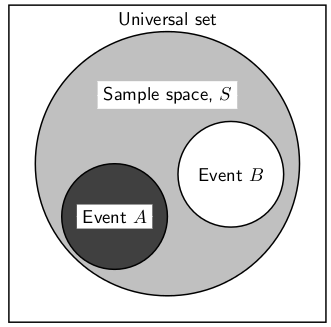
\includegraphics[width=200px]{col11306.imgs/m39377_MG10C17_001.png} % m39377;MG10C17\_001.png;;;6.0;8.5;
        
      \vspace{2pt}
    \vspace{\rubberspace}\par \begin{cnxcaption}
	  \small \textbf{Figure 11.1: }Diagram to show difference between the universal set and
the sample space. The sample space is made up of all possible outcomes of a
statistical experiment and an event is a subset of the sample space.
	\end{cnxcaption}
      
    \vspace{.1in}
    \rule[.1in]{\figurerulewidth}{.005in} \\
        
    \end{center}

 \end{figure}   

    \addtocounter{footnote}{-0}
    
          \label{m39377*eip-451}We can draw Venn diagrams for experiments with two and three events. These are shown in Figure~11.2 and Figure~11.3. Venn diagrams for experiments with more than three events are more complex and are not covered at this level. \par 

    \setcounter{subfigure}{0}


	\begin{figure}[H] % horizontal\label{m39377*uid1211}
    \begin{center}
    \rule[.1in]{\figurerulewidth}{.005in} \\
        \label{m39377*uid1211!!!underscore!!!media}\label{m39377*uid1211!!!underscore!!!printimage}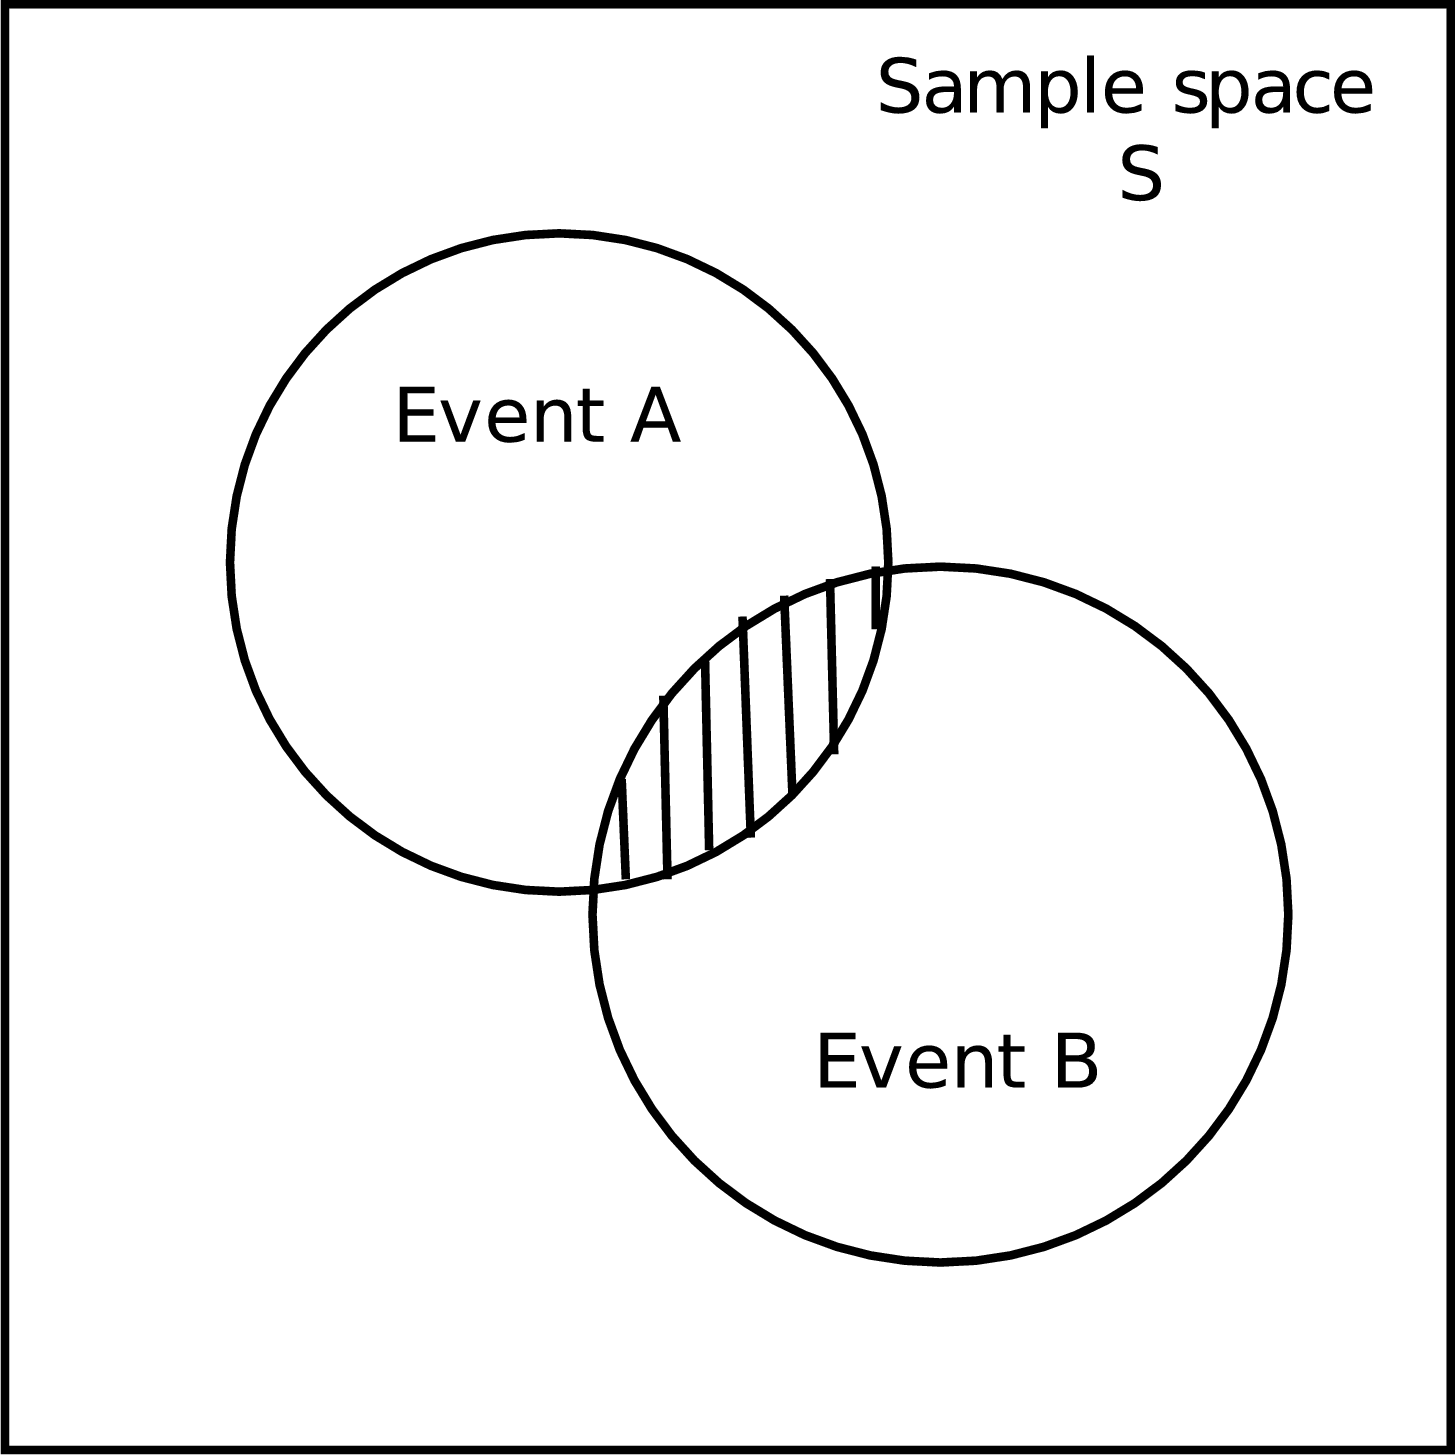
\includegraphics[width=150px]{col11306.imgs/m39377_venn1.png} % m39377;venn1.png;;;6.0;8.5;
        
      \vspace{2pt}
    \vspace{\rubberspace}\par \begin{cnxcaption}
	  \small \textbf{Figure 11.2: }Venn diagram for an experiment with two events
	\end{cnxcaption}
      
    \vspace{.1in}
    \rule[.1in]{\figurerulewidth}{.005in} \\
        
    \end{center}

 \end{figure}   

    \addtocounter{footnote}{-0}
    

    \setcounter{subfigure}{0}


	\begin{figure}[H] % horizontal\label{m39377*uid1222}
    \begin{center}
    \rule[.1in]{\figurerulewidth}{.005in} \\
        \label{m39377*uid1222!!!underscore!!!media}\label{m39377*uid1222!!!underscore!!!printimage}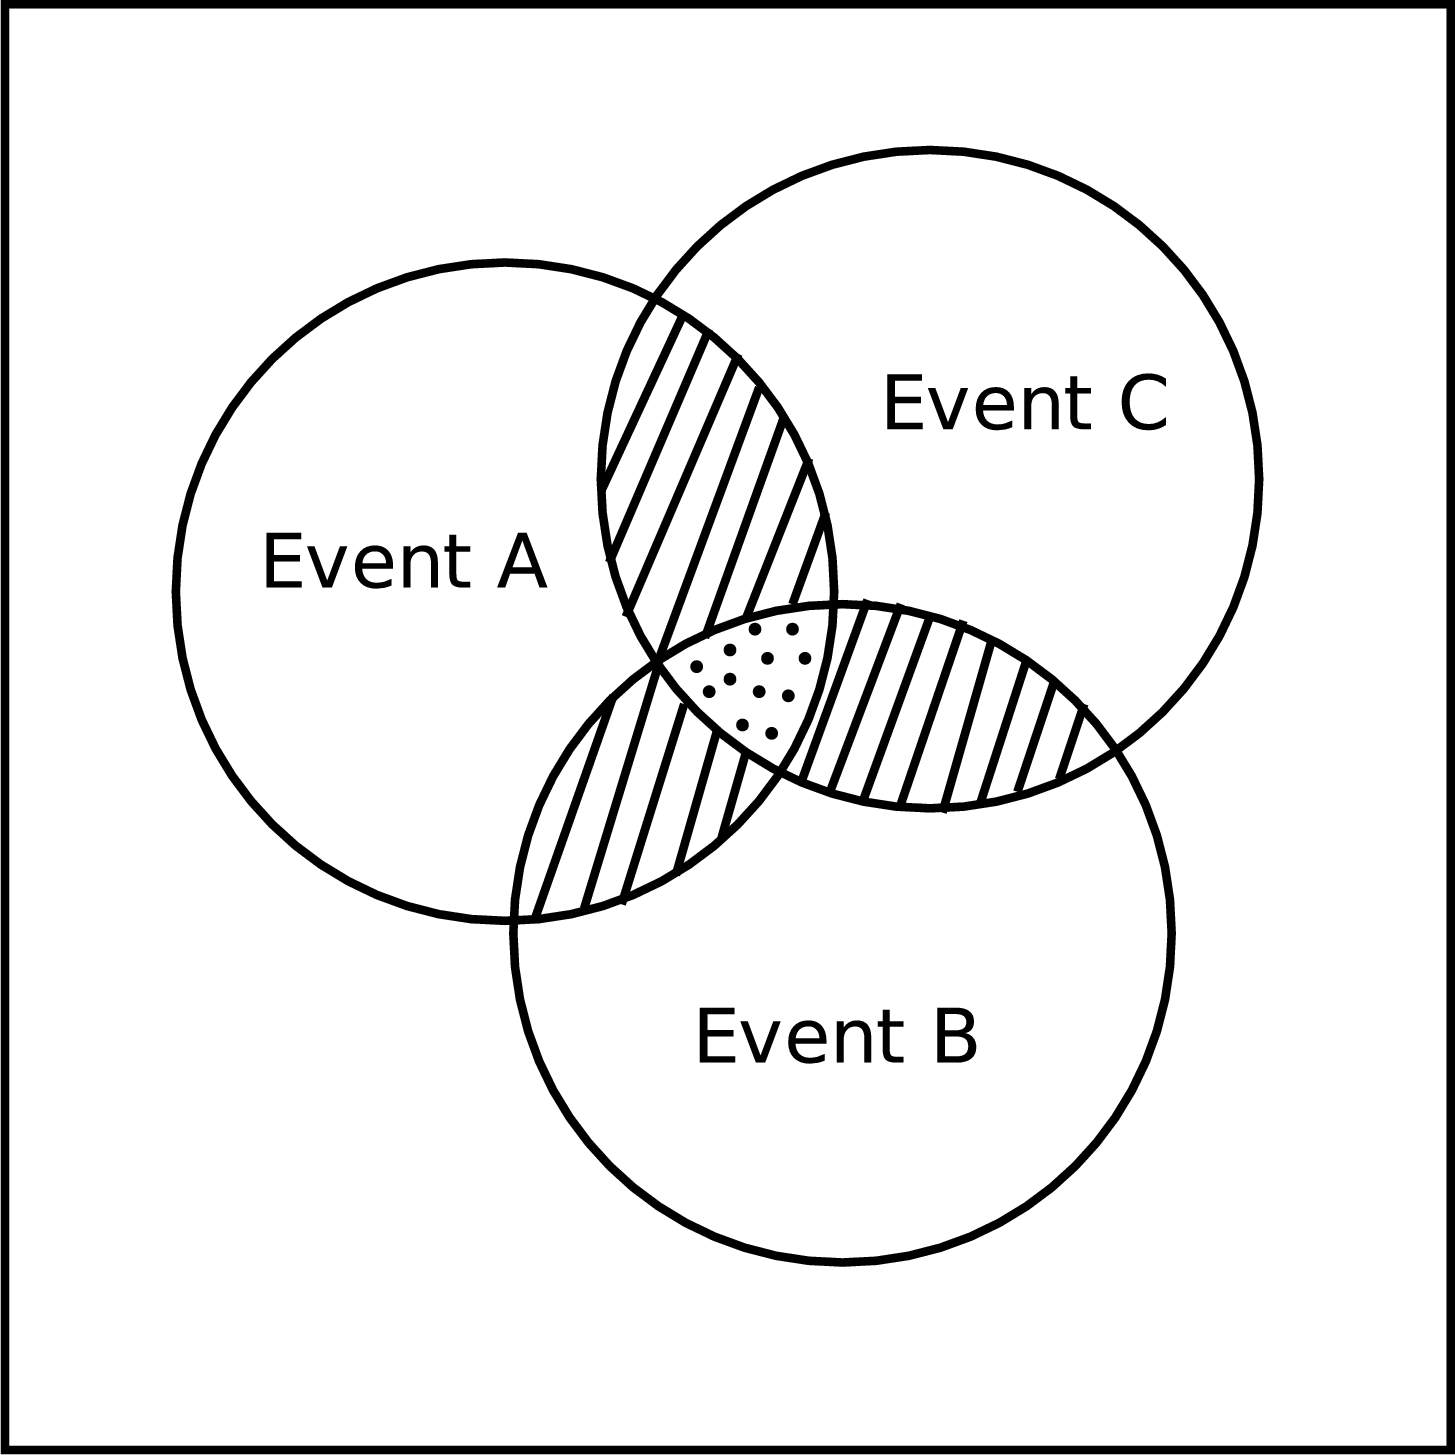
\includegraphics[width=150px]{col11306.imgs/m39377_venn2.png} % m39377;venn2.png;;;6.0;8.5;
        
      \vspace{2pt}
    \vspace{\rubberspace}\par \begin{cnxcaption}
	  \small \textbf{Figure 11.3: }Venn diagram for an experiment with three events.
	\end{cnxcaption}
      
    \vspace{.1in}
    \rule[.1in]{\figurerulewidth}{.005in} \\
        
    \end{center}

 \end{figure}   

    \addtocounter{footnote}{-0}
    
          \label{m39377*eip-568}
\begin{tabular}{cc}
	\hspace*{-50pt}\raisebox{-8 mm}{\hspace{-0.2in}
\includegraphics[width=0.75in]{col11306.imgs/psfact2.png} } & 

	\begin{minipage}{0.85\textwidth}
	\begin{note}
      {note: }The Greek, Russian and Latin alphabets can be illustrated using Venn diagrams. All these alphabets have some common letters. The Venn diagram is given below:

    \setcounter{subfigure}{0}


	\begin{figure}[H] % horizontal\label{m39377*id7888}
    \begin{center}
    \label{m39377*id7888!!!underscore!!!media}\label{m39377*id7888!!!underscore!!!printimage}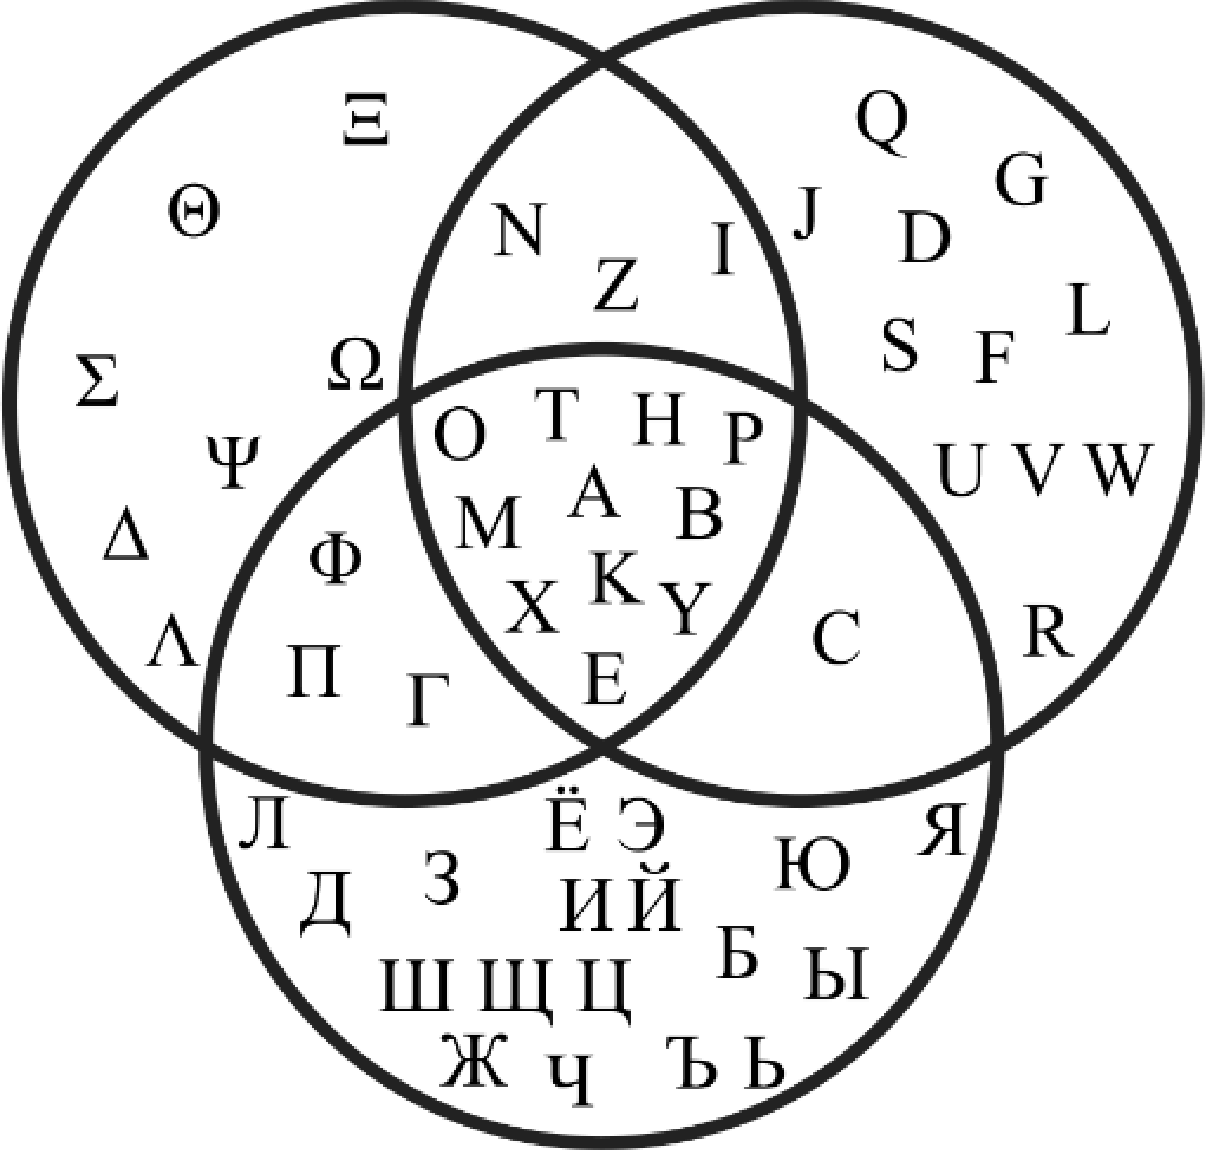
\includegraphics[width=150px]{col11306.imgs/m39377_venn_ifact.png} % m39377;venn\_ifact.png;;;6.0;8.5;
        
      \vspace{2pt}
    \vspace{.1in}
    
    \end{center}

 \end{figure}   

    \addtocounter{footnote}{-0}
    
	\end{note}
	\end{minipage}
	\end{tabular}
	\par
      \label{m39377*eip-256}The \textsl{union} of
\begin{math}A\end{math} and \begin{math}B\end{math} is the set of all elements in \begin{math}A\end{math} or in \begin{math}B\end{math} (or in both). \begin{math}A\phantom{\rule{4pt}{0ex}}\mathbf{or}\phantom{\rule{4pt}{0ex}}B\end{math} is also written \begin{math}A\cup B\end{math}. The \textsl{intersection} of \begin{math}A\end{math} and \begin{math}B\end{math} is the set of all elements in both
\begin{math}A\end{math} and \begin{math}B\end{math}. 
\begin{math}A\phantom{\rule{4pt}{0ex}}\mathbf{and}\phantom{\rule{4pt}{0ex}}B\end{math} is also written as \begin{math}A\cap B\end{math}.\par \label{m39377*eip-429}Venn diagrams can also be used to indicate the
union and intersection between events in a sample space (Figure~11.5 and Figure~11.6).\par 

    \setcounter{subfigure}{0}


	\begin{figure}[H] % horizontal\label{m39377*uid13}
    \begin{center}
    \rule[.1in]{\figurerulewidth}{.005in} \\
        \label{m39377*uid13!!!underscore!!!media}\label{m39377*uid13!!!underscore!!!printimage}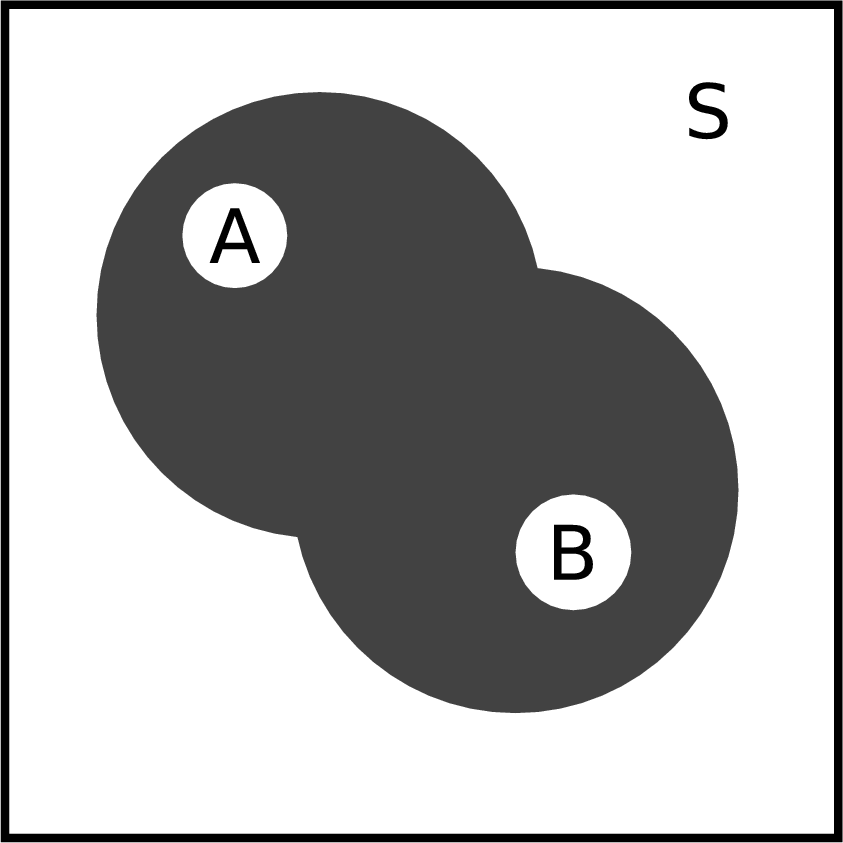
\includegraphics[width=150px]{col11306.imgs/m39377_union.png} % m39377;union.png;;;6.0;8.5;
        
      \vspace{2pt}
    \vspace{\rubberspace}\par \begin{cnxcaption}
	  \small \textbf{Figure 11.5: }Venn diagram to show (left) union of two events, \begin{math}A\end{math} and \begin{math}B\end{math}, in the sample space \begin{math}S\end{math}.
	\end{cnxcaption}
      
    \vspace{.1in}
    \rule[.1in]{\figurerulewidth}{.005in} \\
        
    \end{center}

 \end{figure}   

    \addtocounter{footnote}{-0}
    

    \setcounter{subfigure}{0}


	\begin{figure}[H] % horizontal\label{m39377*uid1381}
    \begin{center}
    \rule[.1in]{\figurerulewidth}{.005in} \\
        \label{m39377*uid1381!!!underscore!!!media}\label{m39377*uid1381!!!underscore!!!printimage}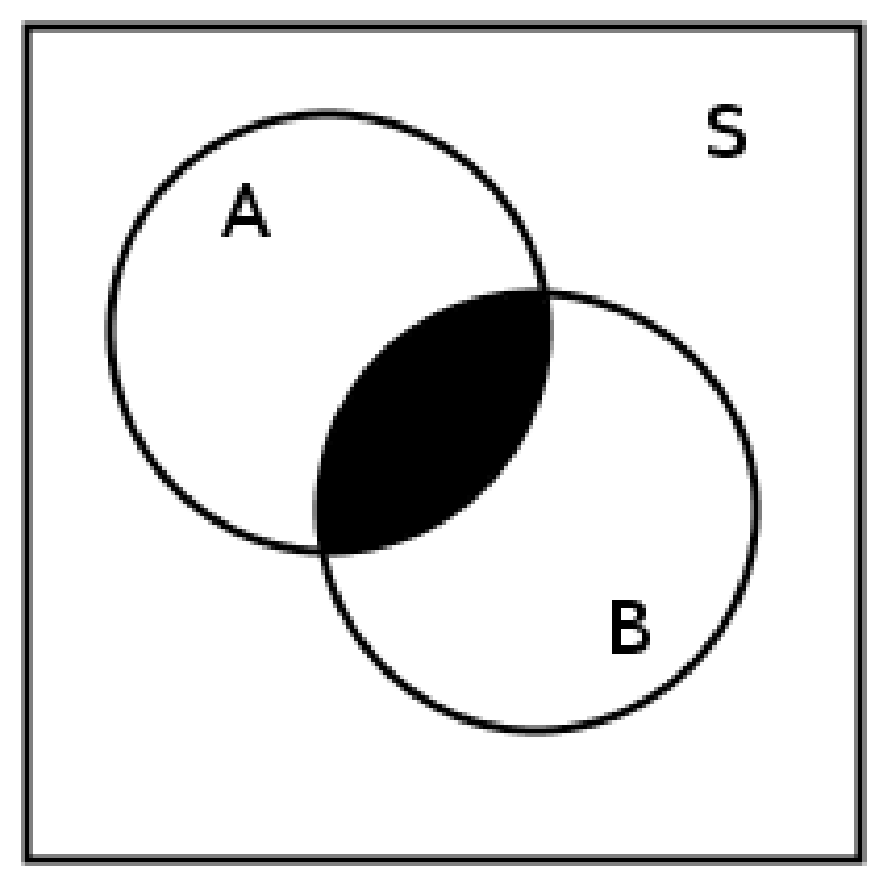
\includegraphics[width=150px]{col11306.imgs/m39377_intersect.png} % m39377;intersect.png;;;6.0;8.5;
        
      \vspace{2pt}
    \vspace{\rubberspace}\par \begin{cnxcaption}
	  \small \textbf{Figure 11.6: }Venn diagram to show intersection of two events
\begin{math}A\end{math} and \begin{math}B\end{math}, in the sample space \begin{math}S\end{math}. The black region indicates the
intersection.
	\end{cnxcaption}
      
    \vspace{.1in}
    \rule[.1in]{\figurerulewidth}{.005in} \\
        
    \end{center}

 \end{figure}   

    \addtocounter{footnote}{-0}
    

\label{m39377*eip-805}We use \begin{math}n\left(S\right)\end{math} to refer to the number of elements in a set \begin{math}S\end{math}, \begin{math}n\left(X\right)\end{math} for the number of elements in \begin{math}X\end{math}, etc.\par \label{m39377*secfhsst!!!underscore!!!id141}\vspace{.5cm} 
      
      \noindent
      \hspace*{-30pt}
\includegraphics[width=0.5in]{col11306.imgs/pspencil2.png}   \raisebox{25mm}{   
      \begin{mdframed}[linewidth=4, leftmargin=40, rightmargin=40]  
      \begin{exercise}
    \noindent\textbf{Exercise 11.1:  Random Experiments }
          \label{m39377*probfhsst!!!underscore!!!id142}
          \label{m39377*id110320}In a box there are pieces of paper with the
numbers from 1 to 9 written on them. A piece of paper is drawn from the box and
the number on it is noted. Let \begin{math}S\end{math}
denote the sample space, let \begin{math}P\end{math}
denote the event 'drawing a prime number', and let \begin{math}E\end{math} denote the event 'drawing an even
number'. Using appropriate notation, in how many ways is it possible to draw: i)
any number? ii) a prime number? iii) an even number? iv) a number that is either
prime or even? v) a number that is both prime and even?\par 
          
          \vspace{5pt}
          \label{m39377*solfhsst!!!underscore!!!id147}\noindent\textbf{Solution to Exercise } \label{m39377*listfhsst!!!underscore!!!id147}\begin{enumerate}[noitemsep, label=\textbf{Step} \textbf{\arabic*}. ] 
            \leftskip=20pt\rightskip=\leftskip\item  
          \label{m39377*id110396}\begin{itemize}[noitemsep]
            \leftskip=20pt\rightskip=\leftskip\label{m39377*uid14}\item Drawing a prime number: \begin{math}P=\{2;3;5;7
\}\end{math}\label{m39377*uid15}\item Drawing an even number: \begin{math}E=\{2;4;6;8
\}\end{math}\end{itemize}
        
          \item  
          \label{m39377*id110666}
            
    \setcounter{subfigure}{0}


	\begin{figure}[H] % horizontal\label{m39377*id110668}
    \begin{center}
    \label{m39377*id110668!!!underscore!!!media}\label{m39377*id110668!!!underscore!!!printimage}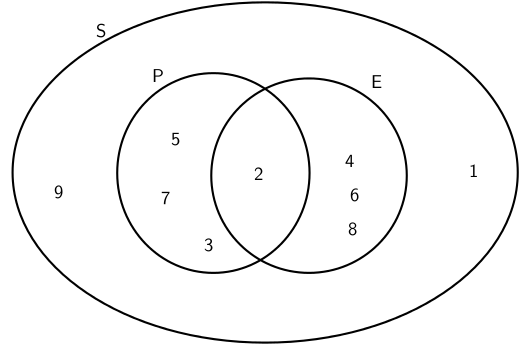
\includegraphics[width=200px]{col11306.imgs/m39377_MG10C17_003.png} % ;MG10C17\_003.png;;;6.0;8.5;
        
      \vspace{2pt}
    \vspace{.1in}
    
    \end{center}

 \end{figure}   

    \addtocounter{footnote}{-0}
    
          \par 
          \item  
          \label{m39377*id110678}The \textsl{union} of
\begin{math}P\end{math} and \begin{math}E\end{math} is the set of all elements in \begin{math}P\end{math} or in \begin{math}E\end{math} (or in both). \begin{math}P\cup E=2,3,4,5,6,7,8\end{math}. \par 
          \item  
          \label{m39377*id110808}The \textsl{intersection} of \begin{math}P\end{math} and \begin{math}E\end{math} is the set of all elements in both
\begin{math}P\end{math} and \begin{math}E\end{math}. \begin{math}P\cap E=2\end{math}.
\par 
          \item  
          
          \label{m39377*id110962}\nopagebreak\noindent{}
            \settowidth{\mymathboxwidth}{\begin{equation}
    \begin{array}{ccc}\hfill \therefore \phantom{\rule{0.166667em}{0ex}}\phantom{\rule{0.166667em}{0ex}}n\left(S\right)& =& 9\hfill \\ \hfill n\left(P\right)& =& 4\hfill \\ \hfill n\left(E\right)& =& 4\hfill \\ \hfill n\left(P\cup E\right)& =& 7\hfill \\ \hfill n\left(P\cap E\right)& =& 2\hfill \end{array}\tag{11.1}
      \end{equation}
    }
    \typeout{Columnwidth = \the\columnwidth}\typeout{math as usual width = \the\mymathboxwidth}
    \ifthenelse{\lengthtest{\mymathboxwidth < \columnwidth}}{% if the math fits, do it again, for real
    \begin{equation}
    \begin{array}{ccc}\hfill \therefore \phantom{\rule{0.166667em}{0ex}}\phantom{\rule{0.166667em}{0ex}}n\left(S\right)& =& 9\hfill \\ \hfill n\left(P\right)& =& 4\hfill \\ \hfill n\left(E\right)& =& 4\hfill \\ \hfill n\left(P\cup E\right)& =& 7\hfill \\ \hfill n\left(P\cap E\right)& =& 2\hfill \end{array}\tag{11.1}
      \end{equation}
    }{% else, if it doesn't fit
    \setlength{\mymathboxwidth}{\columnwidth}
      \addtolength{\mymathboxwidth}{-48pt}
    \par\vspace{12pt}\noindent\begin{minipage}{\columnwidth}
    \parbox[t]{\mymathboxwidth}{\large\begin{math}
    \therefore \phantom{\rule{0.166667em}{0ex}}\phantom{\rule{0.166667em}{0ex}}n\left(S\right)=9n\left(P\right)=4n\left(E\right)=4n\left(P\cup E\right)=7n\left(P\cap E\right)=2\end{math}}\hfill
    \parbox[t]{48pt}{\raggedleft 
    (11.1)}
    \end{minipage}\vspace{12pt}\par
    }% end of conditional for this bit of math
    \typeout{math as usual width = \the\mymathboxwidth}
    
          
          
          \end{enumerate}
         

    \end{exercise}
    \end{mdframed}
    }
    \noindent
  \par
            \label{m39377*eip-756}\vspace{.5cm} 
      
      \noindent
      \hspace*{-30pt}
\includegraphics[width=0.5in]{col11306.imgs/pspencil2.png}   \raisebox{25mm}{   
      \begin{mdframed}[linewidth=4, leftmargin=40, rightmargin=40]  
      \begin{exercise}
    \noindent\textbf{Exercise 11.2}\label{m39377*eip-431}
  \label{m39377*eip-524}
100 people were surveyed to find out which fast food chain (Nandos, Debonairs or Steers) they preferred. The following results were obtained:
\label{m39377*id7536}\begin{itemize}[noitemsep]
            \leftskip=20pt\rightskip=\leftskip\item 50 liked Nandos \item 66 liked Debonairs\item 40 liked Steers\item 27 liked Nandos and Debonairs but not Steers\item 13 liked Debonairs and Steers but not Nandos\item 4 liked all three\item 94 liked at least one\end{itemize}
        
\label{m39377*id76932}\begin{enumerate}[noitemsep, label=\textbf{\alph*}. ] 
            \leftskip=20pt\rightskip=\leftskip\item How many people did not like any of the fast food chains?\item How many people liked Nandos and Steers, but not Debonairs?\end{enumerate}
        
  \par 
\vspace{5pt}

\label{m39377*eip-363}\noindent\textbf{Solution to Exercise }
\label{m39377*id7234}\begin{enumerate}[noitemsep, label=\textbf{Step} \textbf{\arabic*}. ] 
            \leftskip=20pt\rightskip=\leftskip\item 
The number of people who liked Nandos and Debonairs is 27, so this is the intersection of these two events. The number of people who liked Debonairs and Steers is 13, so the intersection of Debonairs and Steers is 13. We are told that 4 people like all three options, and so this means that there are 4 people in the intersection of all three options. So we can work out that the number of people who like just Debonairs is \begin{math}66--4--27-13=22\end{math} (This is simply the total number who like Debonairs minus the number of people who like Debonairs and Steers, or Debonairs and Nandos or all three). 
We draw the following diagram to represent the data:

    \setcounter{subfigure}{0}


	\begin{figure}[H] % horizontal\label{m39377*id1368}
    \begin{center}
    \label{m39377*id1368!!!underscore!!!media}\label{m39377*id1368!!!underscore!!!printimage}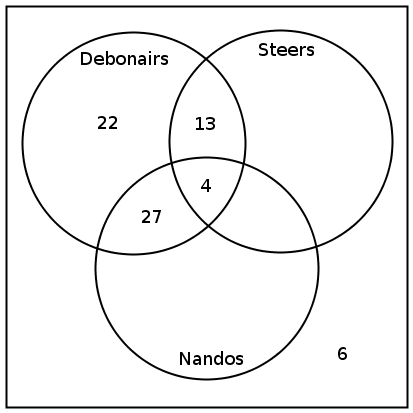
\includegraphics[width=200px]{col11306.imgs/m39377_Vennwex1.png} % ;Vennwex1.png;;;6.0;8.5;
        
      \vspace{2pt}
    \vspace{.1in}
    
    \end{center}

 \end{figure}   

    \addtocounter{footnote}{-0}
    
\item 
We are told that there were 100 people and that 94 liked at least one. So the number of people that liked none is: \begin{math}100--94=6\end{math}. This is the answer to a).
\item 

We can redraw the part of the Venn diagram that is of interest:

    \setcounter{subfigure}{0}


	\begin{figure}[H] % horizontal\label{m39377*id533}
    \begin{center}
    \label{m39377*id533!!!underscore!!!media}\label{m39377*id533!!!underscore!!!printimage}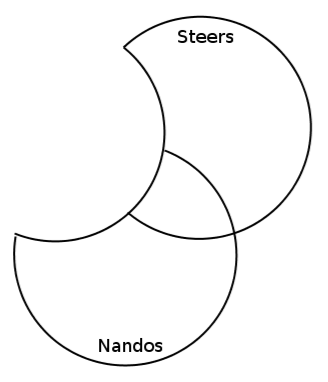
\includegraphics[width=150px]{col11306.imgs/m39377_Vennwex2.png} % ;Vennwex2.png;;;6.0;8.5;
        
      \vspace{2pt}
    \vspace{.1in}
    
    \end{center}

 \end{figure}   

    \addtocounter{footnote}{-0}
    
Total people who like Nandos: 50\newline
    
Of these 27 like both Nandos and Debonairs, and 4 people like all three options. So we find that the total number of people who just like Nandos is: \begin{math}50--27--4=19\end{math}\newline
    
Total people who like Steers: 40\newline
    
Of these 13 like both Steers and Debonairs, and 4 like all three options. So we find that the total number of people who like just Steers is: \begin{math}40--13--4=23\end{math}\newline
    
Now use the identity \begin{math}\mathrm{n\left(N\; or\; S\right)}=\mathrm{n\left(N\right)}+\mathrm{n\left(S\right)}--\mathrm{n\left(N\; and\; S\right)}\end{math} to find the number of people who like Nandos and Steers, but not Debonairs.
\label{m39377*id734}\nopagebreak\noindent{}\settowidth{\mymathboxwidth}{\begin{equation}
    \begin{array}{ccc}\hfill \mathrm{n\left(N\; or\; S\right)}& =& \mathrm{n\left(N\right)}+\mathrm{n\left(S\right)}--\mathrm{n\left(N\; and\; S\right)}\hfill \\ \hfill 28& =& 23+19--\mathrm{n\left(N\; and\; S\right)}\hfill \\ \hfill \mathrm{n\left(N\; and\; S\right)}& =& 14\hfill \end{array}\tag{11.2}
      \end{equation}
    }
    \typeout{Columnwidth = \the\columnwidth}\typeout{math as usual width = \the\mymathboxwidth}
    \ifthenelse{\lengthtest{\mymathboxwidth < \columnwidth}}{% if the math fits, do it again, for real
    \begin{equation}
    \begin{array}{ccc}\hfill \mathrm{n\left(N\; or\; S\right)}& =& \mathrm{n\left(N\right)}+\mathrm{n\left(S\right)}--\mathrm{n\left(N\; and\; S\right)}\hfill \\ \hfill 28& =& 23+19--\mathrm{n\left(N\; and\; S\right)}\hfill \\ \hfill \mathrm{n\left(N\; and\; S\right)}& =& 14\hfill \end{array}\tag{11.2}
      \end{equation}
    }{% else, if it doesn't fit
    \setlength{\mymathboxwidth}{\columnwidth}
      \addtolength{\mymathboxwidth}{-48pt}
    \par\vspace{12pt}\noindent\begin{minipage}{\columnwidth}
    \parbox[t]{\mymathboxwidth}{\large\begin{math}
    \mathrm{n\left(N\; or\; S\right)}=\mathrm{n\left(N\right)}+\mathrm{n\left(S\right)}--\mathrm{n\left(N\; and\; S\right)}28=23+19--\mathrm{n\left(N\; and\; S\right)}\mathrm{n\left(N\; and\; S\right)}=14\end{math}}\hfill
    \parbox[t]{48pt}{\raggedleft 
    (11.2)}
    \end{minipage}\vspace{12pt}\par
    }% end of conditional for this bit of math
    \typeout{math as usual width = \the\mymathboxwidth}
    
The Venn diagram with that represents all this information is given:

    \setcounter{subfigure}{0}


	\begin{figure}[H] % horizontal\label{m39377*id1106}
    \begin{center}
    \label{m39377*id1106!!!underscore!!!media}\label{m39377*id1106!!!underscore!!!printimage}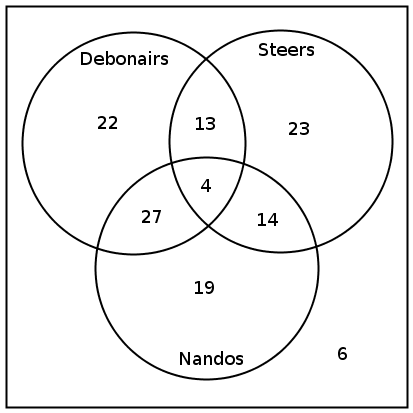
\includegraphics[width=200px]{col11306.imgs/m39377_Vennwex3.png} % ;Vennwex3.png;;;6.0;8.5;
        
      \vspace{2pt}
    \vspace{.1in}
    
    \end{center}

 \end{figure}   

    \addtocounter{footnote}{-0}
    
\end{enumerate}
        


    \end{exercise}
    \end{mdframed}
    }
    \noindent
  
\label{m39377*eip-796}
            \subsubsection{ Activity: Venn diagrams}
            \nopagebreak
            \label{m39377*eip-65}Which cellphone networks have you used or are you signed up for (e.g. Vodacom, Mtn or CellC)? Collect this information from your classmates as well. Then use the information to draw a Venn diagram (if you have more than three networks, then choose only the three most popular or draw Venn diagrams for all the combinations). Try to see if you can work out the number of people who use just one network, or the number of people who use all the networks.
\par \label{m39377*secfhsst!!!underscore!!!id3294}
            \subsubsection{ Complement and complementary events}
            \nopagebreak
            
\label{m39377*eip-442}A final notion that is important to understand is the notion
of \textsl{complement}.
Just as in geometry when two angles are called 'complementary' if they added up
to 90 degrees, (the two angles 'complement' each other to make a right angle), the complement of a set of outcomes \begin{math}A\end{math} is the set of all outcomes in the sample space but not in \begin{math}A\end{math}. It is usually denoted
\begin{math}{A}^{\text{'}}\end{math} (or sometimes \begin{math}{A}^{C}\end{math}), and called 'the complement of \begin{math}A\end{math}' or simply '\begin{math}A\end{math}-complement'. Because it refers to the set of everything outside of \begin{math}A\end{math}, it is also often referred to as 'not-\begin{math}A\end{math}'. Thus, by definition, if \begin{math}S\end{math} denotes the entire sample space of possible outcomes, and \begin{math}A\end{math} is any subset of outcomes that we are interested in (i.e. an \textsl{event}), then \begin{math}A\cup {A}^{\text{'}}=S\end{math} is always
true, (i.e. \begin{math}{A}^{\text{'}}\end{math} \textsl{complements} \begin{math}A\end{math} to form the entire
sample space). So in the exercise above, \begin{math}{P}^{\text{'}}=\{1,4,6,8,9\}\end{math},
while \begin{math}{E}^{\text{'}}=\{1,3,5,7,9\}\end{math}. So \begin{math}n\left({P}^{\text{'}}\right)=n\left({E}^{\text{'}}\right)=5\end{math}\par \label{m39377*eip-324}The probability of a complementary event refers to the
probability associated with the complement of an event, i.e. the probability that something other than the event in question will occur. For example, if \begin{math}P\left(A\right)=0,25\end{math},
then the probability of \begin{math}A\end{math} not
occurring is the probability associated with all other events in \begin{math}S\end{math} occurring less the probability of
\begin{math}A\end{math} occurring.\par \label{m39377*eip-788}In
theory, it is very easy to calculate complements, since the number of elements
in the complement of a set is just the total number of outcomes in the sample
space minus the outcomes in that set (in the example above, there were 9
possible outcomes in the sample space, and 4 possible outcomes in each of the
sets we were interested in, thus both complements contained 9-4 = 5 elements).
Similarly, it is easy to calculate probabilities of complements of events since
they are simply the total probability (e.g. 1 if our total measure is 1) minus the probability of the event in question. So,\par \label{m39377*eip-936}\nopagebreak\noindent{}\settowidth{\mymathboxwidth}{\begin{equation}
    P\left({A}^{\text{'}}\right)=1-P\left(A\right)\tag{11.3}
      \end{equation}
    }
    \typeout{Columnwidth = \the\columnwidth}\typeout{math as usual width = \the\mymathboxwidth}
    \ifthenelse{\lengthtest{\mymathboxwidth < \columnwidth}}{% if the math fits, do it again, for real
    \begin{equation}
    P\left({A}^{\text{'}}\right)=1-P\left(A\right)\tag{11.3}
      \end{equation}
    }{% else, if it doesn't fit
    \setlength{\mymathboxwidth}{\columnwidth}
      \addtolength{\mymathboxwidth}{-48pt}
    \par\vspace{12pt}\noindent\begin{minipage}{\columnwidth}
    \parbox[t]{\mymathboxwidth}{\large\begin{math}
    P\left({A}^{\text{'}}\right)=1-P\left(A\right)\end{math}}\hfill
    \parbox[t]{48pt}{\raggedleft 
    (11.3)}
    \end{minipage}\vspace{12pt}\par
    }% end of conditional for this bit of math
    \typeout{math as usual width = \the\mymathboxwidth}
    
      \label{m39377*eip-836}Sometimes it is much easier to decide the probability of an event occurring by instead calculating the probability that the complementary event will NOT occur. For example, if the process in question was rolling three dice, and the event we were interested in was that at least one of the faces is a one, it is definitely much easier to figure out the probability that not getting a one will not occur than to try to figure out all the possible combinations of three dice where a one does occur!\par \label{m39377*eip-549}\vspace{.5cm} 
      
      \noindent
      \hspace*{-30pt}
\includegraphics[width=0.5in]{col11306.imgs/pspencil2.png}   \raisebox{25mm}{   
      \begin{mdframed}[linewidth=4, leftmargin=40, rightmargin=40]  
      \begin{exercise}
    \noindent\textbf{Exercise 11.3: Complementary events}\label{m39377*probfhsst!!!underscore!!!id1112}
      \label{m39377*id115556}If you throw two dice, one red and one blue, what is
the probability that at least one of them will be a six? \par 
      \vspace{5pt}
      \label{m39377*solfhsst!!!underscore!!!id1115}\noindent\textbf{Solution to Exercise } \label{m39377*listfhsst!!!underscore!!!id1115}\begin{enumerate}[noitemsep, label=\textbf{Step} \textbf{\arabic*}. ] 
            \leftskip=20pt\rightskip=\leftskip\item  
      \label{m39377*id115580}To solve that kind of question, work out the
probability that there will be no six.\par 
      \item  
      \label{m39377*id115588}The probability that the red dice will not be a six is
5/6, and that the blue one will not be a six is also 5/6.\par 
      \item  
      \label{m39377*id115596}So the probability that neither will be a six is
\begin{math}5/6\ensuremath{\times}5/6=25/36\end{math}.\par 
      \item  
      \label{m39377*id115636}So the probability that at least one will be a six is
\begin{math}1-25/36=11/36\end{math}.
 \par 
      \end{enumerate}
         

    \end{exercise}
    \end{mdframed}
    }
    \noindent
  \label{m39377*eip-768}\vspace{.5cm} 
      
      \noindent
      \hspace*{-30pt}
\includegraphics[width=0.5in]{col11306.imgs/pspencil2.png}   \raisebox{25mm}{   
      \begin{mdframed}[linewidth=4, leftmargin=40, rightmargin=40]  
      \begin{exercise}
    \noindent\textbf{Exercise 11.4: Complementary events}\label{m39377*probfhsst!!!underscore!!!id1128}
      \label{m39377*id115691}A bag contains three red balls, five white balls, two
green balls and four blue balls:\par 
      \label{m39377*id115697}1. Calculate the probability that a red ball will be
drawn from the bag.\par 
      \label{m39377*id115703}2. Calculate the probability that a ball which is not
red will be drawn  \par 
      \vspace{5pt}
      \label{m39377*solfhsst!!!underscore!!!id1133}\noindent\textbf{Solution to Exercise } \label{m39377*listfhsst!!!underscore!!!id1133}\begin{enumerate}[noitemsep, label=\textbf{Step} \textbf{\arabic*}. ] 
            \leftskip=20pt\rightskip=\leftskip\item  
      \label{m39377*id115727}Let R be the event that a red ball is drawn:\par 
      \label{m39377*id115731}\begin{itemize}[noitemsep]
            \leftskip=20pt\rightskip=\leftskip\label{m39377*uid100}\item P(R)-n(R)/n(S)=3/14
\label{m39377*uid101}\item R and R' are complementary events
\end{itemize}
        
      \item  
      \label{m39377*id115764}\begin{math}\therefore \end{math}
P(R') = 1 - P(R) = 1 -3/14 = 11/14\par 
      \item  
      \label{m39377*id115780}\begin{itemize}[noitemsep]
            \leftskip=20pt\rightskip=\leftskip\label{m39377*uid102}\item Alternately P(R') = P(B) + P(W) + P(G)
\label{m39377*uid103}\item P(R') = 4/14 + 5/14 + 2/14 = 11/14
\end{itemize}
        
      
      \end{enumerate}
         

    \end{exercise}
    \end{mdframed}
    }
    \noindent
  
 \label{m39377*cid4}
            \subsubsection{ Probability in Everyday Life}
            \nopagebreak
            
      
      
      \label{m39377*id111785}Probability is connected with uncertainty. In any
statistical experiment, the outcomes that occur may be known, but exactly which
one might not be known. Mathematically, probability theory formulates incomplete
knowledge related to the likelihood of an occurrence. For example, a
meteorologist might say there is a 60\% chance that it will rain tomorrow. This
means that in 6 of every 10 times when the world is in the current state, it
will rain tomorrow.\par 
      
      \label{m39377*id111800}Another way of referring to probabilities is odds. The
odds of an event is defined as the ratio of the probability that the event
occurs to the probability that it does not occur. For example, the odds of a
coin landing on a given side are \begin{math}\frac{0.5}{0.5}=1\end{math}, usually written "1 to 1"
or "1:1". This means that on average, the coin will land on that side as many
times as it will land on the other side.\par 
      \label{m39377*uid36}
            \subsubsection{ The Simplest Example: Equally Likely Outcomes}
            \nopagebreak
            
        
         \label{m39377*eip-953}We say two outcomes are \textsl{equally likely} if they have an equal chance of
happening. For example when a fair coin is tossed, each outcome in the sample
space \begin{math}S=\{heads,tails\}\end{math} is equally likely to occur.\par \label{m39377*eip-594}Probability is a function of events (since it is not possible to have a single event with two different probabilities occurring), so we usually denote the probability \begin{math}P\end{math} of some event \begin{math}E\end{math} occurring by \begin{math}P\left(E\right)\end{math}. When all the outcomes are equally likely (in any
activity), it is fairly straightforward to count the probability of a certain
event occuring. In this case,\par \label{m39377*eip-56}\begin{math}P\left(E\right)=n\left(E\right)/n\left(S\right)\end{math}\par 
        \label{m39377*eip-525}For example, when you throw a fair die the sample
space is \begin{math}S=\{1;2;3;4;5;6\}\end{math} so the total number of possible outcomes \begin{math}n\left(S\right)=6\end{math}.\par \label{m39377*id111979}\textbf{Event 1: Get a 4}
        \par 
        \label{m39377*id111985}The only possible outcome is a 
\begin{math}4\end{math}, i.e \begin{math}E=\{4\}\end{math}. So \begin{math}n\left(E\right)=1\end{math}.
\par 
        \label{m39377*id111992}Probability of getting a 4: \begin{math}P\left(k=4\right)=n\left(E\right)/n\left(S\right)=1/6\end{math}.\par 
        \label{m39377*id111998}\textbf{Event 2: Get a number greater than 3}
        \par 
        \label{m39377*id112007}Favourable outcomes: \begin{math}E=\{4;5;6\}\end{math}\par 
        \label{m39377*id112039}Number of favourable outcomes: \begin{math}n\left(E\right)=3\end{math}.\par 
        \label{m39377*id112045}Probability of getting a number greater than 3:
\begin{math}P\left(k\greatthan{}3\right)=n\left(E\right)/n\left(S\right)=3/6=1/2\end{math}.\par 
\label{m39377*secfhsst!!!underscore!!!id319}\vspace{.5cm} 
      
      \noindent
      \hspace*{-30pt}
\includegraphics[width=0.5in]{col11306.imgs/pspencil2.png}   \raisebox{25mm}{   
      \begin{mdframed}[linewidth=4, leftmargin=40, rightmargin=40]  
      \begin{exercise}
    \noindent\textbf{Exercise 11.5}\label{m39377*probfhsst!!!underscore!!!id320}
        \label{m39377*id112064}A standard deck of cards (without jokers) has 52
cards. There are four sets of cards, called suits. The suit a card belongs to is
denoted by a symbol on the card, the four possible symbols being hearts, clubs,
spades, and diamonds. In each suit there are 13 cards (\begin{math}4\phantom{\rule{4pt}{0ex}}\mathrm{suits}\phantom{\rule{4pt}{0ex}}\ensuremath{\times}\phantom{\rule{4pt}{0ex}}13\phantom{\rule{4pt}{0ex}}\mathrm{cards}=52\end{math}) consisting of one each
of ace, king, queen, jack, and the numbers 2-10.\par 
        \label{m39377*id112108}If we randomly draw a card from the deck, we can the
card drawn as a possible outcome. Therefore, there are 52 possible outcomes. We
can now look at various events and calculate their probabilities:\par 
        \label{m39377*id112113}\begin{enumerate}[noitemsep, label=\textbf{\arabic*}. ] 
            \leftskip=20pt\rightskip=\leftskip\label{m39377*uid39}\item Out of the 52 cards, there are 13 clubs. Therefore,
if the event of interest is drawing a club, there are 13 favourable outcomes,
what is the probability of this event?
\label{m39377*uid40}\item There are 4 kings (one of each suit). The probability
of drawing a king is?
\label{m39377*uid41}\item What is the probability of getting a king or a club?\end{enumerate}
        
        
        \vspace{5pt}
        \label{m39377*solfhsst!!!underscore!!!id333}\noindent\textbf{Solution to Exercise } \label{m39377*listfhsst!!!underscore!!!id333}\begin{enumerate}[noitemsep, label=\textbf{Step} \textbf{\arabic*}. ] 
            \leftskip=20pt\rightskip=\leftskip\item  
        \label{m39377*id112177}The probability of this event is \begin{math}\frac{13}{52}=\frac{1}{4}\end{math}.\par 
        \item  
        \label{m39377*id112208}\begin{math}\frac{4}{52}=\frac{1}{13}\end{math}.\par 
        \item  
        \label{m39377*id112236}This example is slightly more complicated. We cannot
simply add together the number of outcomes for each event separately
(4 + 13 = 17) as this inadvertently counts one of the outcomes twice (the king
of clubs). Why is this so? Well, mathematically if \begin{math}A\end{math} and \begin{math}B\end{math} are two events, it is actually true that 
\begin{math}n\left(A\cup B\right)=n\left(A\right)+n\left(B\right)-n\left(A\cap B\right)\end{math} (a more detailed explanation of this identity is provided below, but for now just assume that it is true). In the results involving the
throwing of dice, the intersection of any two outcomes was empty (and hence
\begin{math}n\left(A\cap B\right)=0\end{math})
since it is not possible for the top face of a die to have two different values
simultaneously. However, in this case, a card can be both a club and a king at
the same time (i.e. \begin{math}n\left(A\cap B\right)=1\end{math}).
Therefore, \begin{math}n\left(A\cup B\right)=4+13-1=16\end{math}. So the correct answer is \begin{math}\frac{16}{52}\end{math}.
 \par 
        \end{enumerate}
         

    \end{exercise}
    \end{mdframed}
    }
    \noindent
  
\label{m39377*secfhsst!!!underscore!!!id343}
            \subsubsection{  Probability Models
}
            \nopagebreak
            
        \label{m39377*id112273}\begin{enumerate}[noitemsep, label=\textbf{\arabic*}. ] 
            \label{m39377*uid42}\item A bag contains 6 red, 3 blue, 2 green and 1 white balls. A ball is
picked at random. What is the probablity that it is:
\label{m39377*id112289}\begin{enumerate}[noitemsep, label=\textbf{\alph*}. ] 
            \label{m39377*uid43}\item red
\label{m39377*uid44}\item blue or white
\label{m39377*uid45}\item not green (hint: think 'complement')
\label{m39377*uid46}\item not green or red?
\end{enumerate}
                \label{m39377*uid47}\item A card is selected randomly from a pack of 52. What
is the probability that it is:
\label{m39377*id112354}\begin{enumerate}[noitemsep, label=\textbf{\alph*}. ] 
            \label{m39377*uid48}\item the 2 of hearts
\label{m39377*uid49}\item a red card
\label{m39377*uid50}\item a picture card
\label{m39377*uid51}\item an ace
\label{m39377*uid52}\item a number less than 4?
\end{enumerate}
                \label{m39377*uid53}\item Even numbers from 2 -100 are written on cards. What
is the probability of selecting a multiple of 5, if a card is drawn at
random?\newline
            
\end{enumerate}
        
        


    
  \label{m39377*cid7}
\par \raisebox{-5 pt}{
\includegraphics[width=0.5cm]{col11306.imgs/summary_www.png}} Find the answers with the shortcodes:
 \par \begin{tabular}[h]{cccccc}
 (1.) lqu  &  (2.) lqJ  &  (3.) lqS  & \end{tabular}



            \section{ Probability Identities}
            \nopagebreak
            \label{m39377*id113940}The following results apply to probabilities, for the sample space
\begin{math}S\end{math} and two events \begin{math}A\end{math} and \begin{math}B\end{math}, within \begin{math}S\end{math}.\par 
      \label{m39377*uid57}\nopagebreak\noindent{}
        \settowidth{\mymathboxwidth}{\begin{equation}
    P\left(S\right)=1\tag{11.4}
      \end{equation}
    }
    \typeout{Columnwidth = \the\columnwidth}\typeout{math as usual width = \the\mymathboxwidth}
    \ifthenelse{\lengthtest{\mymathboxwidth < \columnwidth}}{% if the math fits, do it again, for real
    \begin{equation}
    P\left(S\right)=1\tag{11.4}
      \end{equation}
    }{% else, if it doesn't fit
    \setlength{\mymathboxwidth}{\columnwidth}
      \addtolength{\mymathboxwidth}{-48pt}
    \par\vspace{12pt}\noindent\begin{minipage}{\columnwidth}
    \parbox[t]{\mymathboxwidth}{\large\begin{math}
    P\left(S\right)=1\end{math}}\hfill
    \parbox[t]{48pt}{\raggedleft 
    (11.4)}
    \end{minipage}\vspace{12pt}\par
    }% end of conditional for this bit of math
    \typeout{math as usual width = \the\mymathboxwidth}
    
      
      \label{m39377*uid58}\nopagebreak\noindent{}
        \settowidth{\mymathboxwidth}{\begin{equation}
    P\left(A\cap B\right)=P\left(A\right)\ensuremath{\times}P\left(B\right)\tag{11.5}
      \end{equation}
    }
    \typeout{Columnwidth = \the\columnwidth}\typeout{math as usual width = \the\mymathboxwidth}
    \ifthenelse{\lengthtest{\mymathboxwidth < \columnwidth}}{% if the math fits, do it again, for real
    \begin{equation}
    P\left(A\cap B\right)=P\left(A\right)\ensuremath{\times}P\left(B\right)\tag{11.5}
      \end{equation}
    }{% else, if it doesn't fit
    \setlength{\mymathboxwidth}{\columnwidth}
      \addtolength{\mymathboxwidth}{-48pt}
    \par\vspace{12pt}\noindent\begin{minipage}{\columnwidth}
    \parbox[t]{\mymathboxwidth}{\large\begin{math}
    P\left(A\cap B\right)=P\left(A\right)\ensuremath{\times}P\left(B\right)\end{math}}\hfill
    \parbox[t]{48pt}{\raggedleft 
    (11.5)}
    \end{minipage}\vspace{12pt}\par
    }% end of conditional for this bit of math
    \typeout{math as usual width = \the\mymathboxwidth}
    
      
      \label{m39377*uid59}\nopagebreak\noindent{}
        \settowidth{\mymathboxwidth}{\begin{equation}
    P\left(A\cup B\right)=P\left(A\right)+P\left(B\right)-P\left(A\cap B\right)\tag{11.6}
      \end{equation}
    }
    \typeout{Columnwidth = \the\columnwidth}\typeout{math as usual width = \the\mymathboxwidth}
    \ifthenelse{\lengthtest{\mymathboxwidth < \columnwidth}}{% if the math fits, do it again, for real
    \begin{equation}
    P\left(A\cup B\right)=P\left(A\right)+P\left(B\right)-P\left(A\cap B\right)\tag{11.6}
      \end{equation}
    }{% else, if it doesn't fit
    \setlength{\mymathboxwidth}{\columnwidth}
      \addtolength{\mymathboxwidth}{-48pt}
    \par\vspace{12pt}\noindent\begin{minipage}{\columnwidth}
    \parbox[t]{\mymathboxwidth}{\large\begin{math}
    P\left(A\cup B\right)=P\left(A\right)+P\left(B\right)-P\left(A\cap B\right)\end{math}}\hfill
    \parbox[t]{48pt}{\raggedleft 
    (11.6)}
    \end{minipage}\vspace{12pt}\par
    }% end of conditional for this bit of math
    \typeout{math as usual width = \the\mymathboxwidth}
    
      
\label{m39377*eip-41}We can demonstrate this last result using a Venn diagram. The union of A and B is the set of all elements in A or in B or in both.

    \setcounter{subfigure}{0}


	\begin{figure}[H] % horizontal\label{m39377*id743}
    \begin{center}
    \label{m39377*uid743!!!underscore!!!media}\label{m39377*uid743!!!underscore!!!printimage}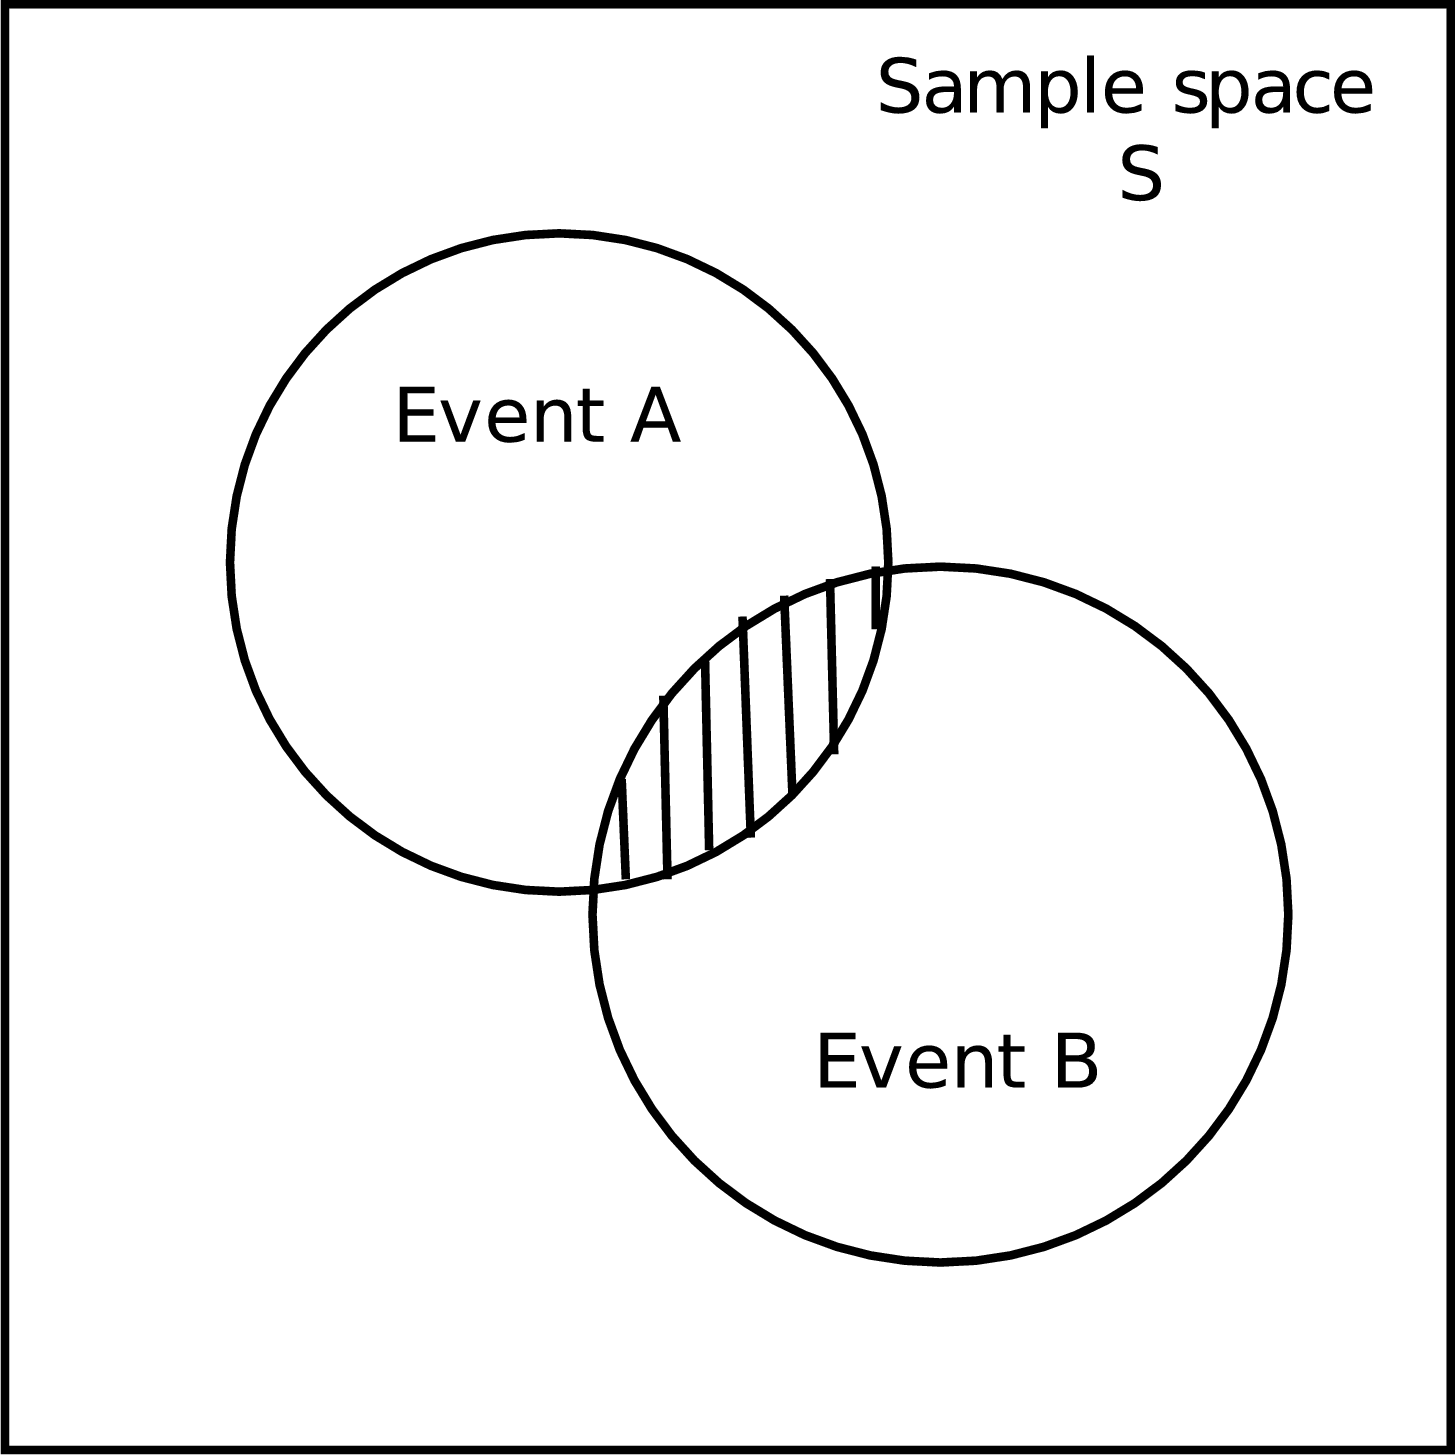
\includegraphics[width=150px]{col11306.imgs/m39377_venn1.png} % m39377;venn1.png;;;6.0;8.5;
        
      \vspace{2pt}
    \vspace{.1in}
    
    \end{center}

 \end{figure}   

    \addtocounter{footnote}{-0}
    
\par \label{m39377*eip-227}The probability of event A occurring is given by \begin{math}\mathrm{P\left(A\right)}\end{math} and the probability of event B occurring is given by \begin{math}\mathrm{P\left(B\right)}\end{math}. However, if we look closely at the circle representing either of these events, we notice that the probability includes a small part of the other event. So event A includes a bit of event B and vice versa. This is shown in the following figure:

    \setcounter{subfigure}{0}


	\begin{figure}[H] % horizontal\label{m39377*id1112}
    \begin{center}
    \label{m39377*id1112!!!underscore!!!media}\label{m39377*id1112!!!underscore!!!printimage}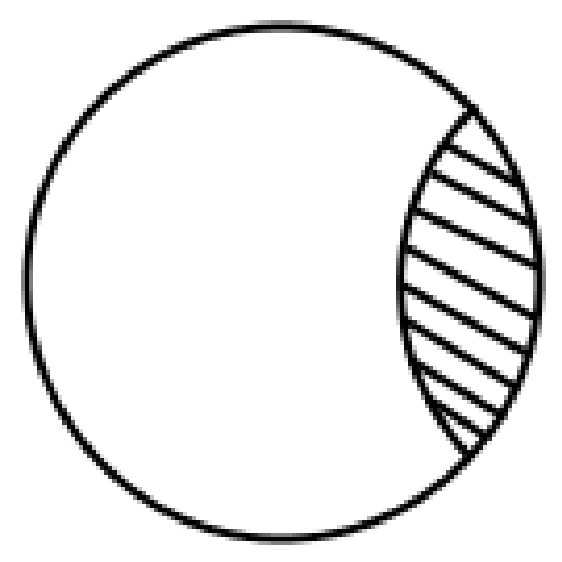
\includegraphics[width=100px]{col11306.imgs/m39377_identity1.png} % m39377;identity1.png;;;6.0;8.5;
        
      \vspace{2pt}
    \vspace{.1in}
    
    \end{center}

 \end{figure}   

    \addtocounter{footnote}{-0}
    
And then we observe that this small bit is simply the intersection of the two events.\par \label{m39377*eip-609}So to find the probability of \begin{math}P\left(A\cup B\right)\end{math} we notice the following: \label{m39377*id9324}\begin{itemize}[noitemsep]
            \item We can add  \begin{math}P\left(A\right)\end{math} and  \begin{math}P\left(B\right)\end{math}\item Doing this counts the intersection twice, once in \begin{math}P\left(A\right)\end{math} and once in \begin{math}P\left(B\right)\end{math}.\end{itemize}
        
So if we simply subtract the probability of the intersection, then we will find the total probability of the union: 

\begin{math}P\left(A\cup B\right)=P\left(A\right)+P\left(B\right)-P\left(A\cap B\right)\end{math}\par \par
            \label{m39377*secfhsst!!!underscore!!!id850}\vspace{.5cm} 
      
      \noindent
      \hspace*{-30pt}
\includegraphics[width=0.5in]{col11306.imgs/pspencil2.png}   \raisebox{25mm}{   
      \begin{mdframed}[linewidth=4, leftmargin=40, rightmargin=40]  
      \begin{exercise}
    \noindent\textbf{Exercise 11.6: Probabilty identities }\label{m39377*probfhsst!!!underscore!!!id851}
      \label{m39377*id114130}What is the probability of selecting a black or red
card from a pack of 52 cards \par 
      \vspace{5pt}
      \label{m39377*solfhsst!!!underscore!!!id854}\noindent\textbf{Solution to Exercise } \label{m39377*listfhsst!!!underscore!!!id854}\begin{enumerate}[noitemsep, label=\textbf{Step} \textbf{\arabic*}. ] 
            \leftskip=20pt\rightskip=\leftskip\item  
      \label{m39377*id114154}\begin{math}P\left(S\right)=\frac{n\left(E\right)}{n\left(S\right)}=\frac{52}{52}=1\end{math} because all cards are black or
red!
 \par 
      \end{enumerate}
         

    \end{exercise}
    \end{mdframed}
    }
    \noindent
  
\label{m39377*secfhsst!!!underscore!!!id860}\vspace{.5cm} 
      
      \noindent
      \hspace*{-30pt}
\includegraphics[width=0.5in]{col11306.imgs/pspencil2.png}   \raisebox{25mm}{   
      \begin{mdframed}[linewidth=4, leftmargin=40, rightmargin=40]  
      \begin{exercise}
    \noindent\textbf{Exercise 11.7:  Probabilty identities }
      \label{m39377*probfhsst!!!underscore!!!id861}
      \label{m39377*id114183}What is the probability of drawing a club or an ace
with one single pick from a pack of 52 cards \par 
      \vspace{5pt}
      \label{m39377*solfhsst!!!underscore!!!id864}\noindent\textbf{Solution to Exercise } \label{m39377*listfhsst!!!underscore!!!id864}\begin{enumerate}[noitemsep, label=\textbf{Step} \textbf{\arabic*}. ] 
            \leftskip=20pt\rightskip=\leftskip\item  
      \label{m39377*id114207}\nopagebreak\noindent{}
        \settowidth{\mymathboxwidth}{\begin{equation}
    P\left(\mathrm{club}\cup \mathrm{ace}\right)=\mathrm{P}\left(\mathrm{club}\right)+\mathrm{P}\left(\mathrm{ace}\right)-\mathrm{P}\left(\mathrm{club}\cap \mathrm{ace}\right)\tag{11.7}
      \end{equation}
    }
    \typeout{Columnwidth = \the\columnwidth}\typeout{math as usual width = \the\mymathboxwidth}
    \ifthenelse{\lengthtest{\mymathboxwidth < \columnwidth}}{% if the math fits, do it again, for real
    \begin{equation}
    P\left(\mathrm{club}\cup \mathrm{ace}\right)=\mathrm{P}\left(\mathrm{club}\right)+\mathrm{P}\left(\mathrm{ace}\right)-\mathrm{P}\left(\mathrm{club}\cap \mathrm{ace}\right)\tag{11.7}
      \end{equation}
    }{% else, if it doesn't fit
    \setlength{\mymathboxwidth}{\columnwidth}
      \addtolength{\mymathboxwidth}{-48pt}
    \par\vspace{12pt}\noindent\begin{minipage}{\columnwidth}
    \parbox[t]{\mymathboxwidth}{\large\begin{math}
    P\left(\mathrm{club}\cup \mathrm{ace}\right)=\mathrm{P}\left(\mathrm{club}\right)+\mathrm{P}\left(\mathrm{ace}\right)-\mathrm{P}\left(\mathrm{club}\cap \mathrm{ace}\right)\end{math}}\hfill
    \parbox[t]{48pt}{\raggedleft 
    (11.7)}
    \end{minipage}\vspace{12pt}\par
    }% end of conditional for this bit of math
    \typeout{math as usual width = \the\mymathboxwidth}
    
      
      \item  
      \label{m39377*id114279}\nopagebreak\noindent{}
        \settowidth{\mymathboxwidth}{\begin{equation}
    \begin{array}{ccc}& =& \frac{1}{4}+\frac{1}{13}-\left(\frac{1}{4}\ensuremath{\times}\frac{1}{13}\right)\hfill \\ & =& \frac{1}{4}+\frac{1}{13}-\frac{1}{52}\hfill \\ & =& \frac{16}{52}\hfill \\ & =& \frac{4}{13}\hfill \end{array}\tag{11.8}
      \end{equation}
    }
    \typeout{Columnwidth = \the\columnwidth}\typeout{math as usual width = \the\mymathboxwidth}
    \ifthenelse{\lengthtest{\mymathboxwidth < \columnwidth}}{% if the math fits, do it again, for real
    \begin{equation}
    \begin{array}{ccc}& =& \frac{1}{4}+\frac{1}{13}-\left(\frac{1}{4}\ensuremath{\times}\frac{1}{13}\right)\hfill \\ & =& \frac{1}{4}+\frac{1}{13}-\frac{1}{52}\hfill \\ & =& \frac{16}{52}\hfill \\ & =& \frac{4}{13}\hfill \end{array}\tag{11.8}
      \end{equation}
    }{% else, if it doesn't fit
    \setlength{\mymathboxwidth}{\columnwidth}
      \addtolength{\mymathboxwidth}{-48pt}
    \par\vspace{12pt}\noindent\begin{minipage}{\columnwidth}
    \parbox[t]{\mymathboxwidth}{\large\begin{math}
    =\frac{1}{4}+\frac{1}{13}-\left(\frac{1}{4}\ensuremath{\times}\frac{1}{13}\right)=\frac{1}{4}+\frac{1}{13}-\frac{1}{52}=\frac{16}{52}=\frac{4}{13}\end{math}}\hfill
    \parbox[t]{48pt}{\raggedleft 
    (11.8)}
    \end{minipage}\vspace{12pt}\par
    }% end of conditional for this bit of math
    \typeout{math as usual width = \the\mymathboxwidth}
    
      
      \label{m39377*id114403}Notice how we have used \begin{math}P\left(C\cup A\right)=P\left(C\right)+P\left(A\right)-P\left(C\cap A\right)\end{math}.
 \par 
      \end{enumerate}
         

    \end{exercise}
    \end{mdframed}
    }
    \noindent
  
\label{m39377*eip-778}The following video provides a brief summary of some of the
work covered so far.

    \setcounter{subfigure}{0}


	\begin{figure}[H] % horizontal\label{m39377*uid333}
    
    
    \textnormal{Khan academy video on
probability}\vspace{.1in} \nopagebreak
  \label{m39377*yt-media}\label{m39377*yt-video}
            \raisebox{-5 pt}{ 
\includegraphics[width=0.5cm]{col11306.imgs/summary_www.png}} { (Video:  MG10085 )}
      
      \vspace{2pt}
    \vspace{.1in}
    
    

 \end{figure}   

    \addtocounter{footnote}{-0}
    \par \label{m39377*secfhsst!!!underscore!!!id985}
            \subsubsection{ Exercise: Probability Identities
}
            \nopagebreak
            
      \label{m39377*id114484}Answer the following questions \par 
      \label{m39377*id114495}\begin{enumerate}[noitemsep, label=\textbf{\arabic*}. ] 
            \label{m39377*uid60}\item Rory is target shooting. His probability of hitting the target is
\begin{math}0,7\end{math}. He fires five shots. What is the probability
that all five shots miss the center?\newline
            \label{m39377*uid63}\item An archer is shooting arrows at a bullseye. The
probability that an arrow hits the bullseye is
\begin{math}0,4\end{math}. If she fires three arrows, what is the
probability that all the arrows hit the bullseye?\newline
            \label{m39377*uid66}\item A dice with the numbers 1,3,5,7,9,11 on it is rolled.
Also a fair coin is tossed. What is the probability that:
\label{m39377*id114596}\begin{enumerate}[noitemsep, label=\textbf{\alph*}. ] 
            \label{m39377*uid69}\item A tail is tossed and a 9 rolled?
\label{m39377*uid70}\item A head is tossed and a 3 rolled?
\end{enumerate}
                \label{m39377*uid71}\item Four children take a test. The probability of each one
passing is as follows. Sarah: \begin{math}0,8\end{math}, Kosma:
\begin{math}0,5\end{math}, Heather: \begin{math}0,6\end{math},
Wendy: \begin{math}0,9\end{math}. What is the probability that:
\label{m39377*id114667}\begin{enumerate}[noitemsep, label=\textbf{\alph*}. ] 
            \label{m39377*uid72}\item all four pass?
\label{m39377*uid73}\item all four fail?
\end{enumerate}
                \label{m39377*uid75}\item With a single pick from a pack of 52 cards what is the
probability that the card will be an ace or a black card?\newline
            
\end{enumerate}
        
    
    \label{m39377*cid8}
\par \raisebox{-5 pt}{
\includegraphics[width=0.5cm]{col11306.imgs/summary_www.png}} Find the answers with the shortcodes:
 \par \begin{tabular}[h]{cccccc}
 (1.) lab  &  (2.) laj  &  (3.) laD  &  (4.) laW  &  (5.) laZ  & \end{tabular}



            \section{ Mutually Exclusive Events}
            \nopagebreak
            \label{m39377*id114732}Two events are called mutually exclusive if they cannot be
true at the same time.\par 
      \label{m39377*id114736}Examples of mutually exclusive events are:\par 
      \label{m39377*id114740}\begin{enumerate}[noitemsep, label=\textbf{\arabic*}. ] 
            \label{m39377*uid76}\item A die landing on an even number or landing on an odd
number.
\label{m39377*uid77}\item A student passing or failing an exam
\label{m39377*uid78}\item A tossed coin landing on heads or landing on tails
\end{enumerate}
        
      \label{m39377*id114782}This means that if we examine the elements of the sets
that make up \begin{math}A\end{math} and \begin{math}B\end{math} there will be no elements in common.
Therefore, \begin{math}A\cap B=\varnothing \end{math} (where \begin{math}\varnothing \end{math} refers to the empty set). Since,
\begin{math}P\left(A\cap B\right)=0\end{math},
equation (11.6) becomes:\par 
      \label{m39377*id114861}\nopagebreak\noindent{}
        \settowidth{\mymathboxwidth}{\begin{equation}
    P\left(A\cup B\right)=P\left(A\right)+P\left(B\right)\tag{11.9}
      \end{equation}
    }
    \typeout{Columnwidth = \the\columnwidth}\typeout{math as usual width = \the\mymathboxwidth}
    \ifthenelse{\lengthtest{\mymathboxwidth < \columnwidth}}{% if the math fits, do it again, for real
    \begin{equation}
    P\left(A\cup B\right)=P\left(A\right)+P\left(B\right)\tag{11.9}
      \end{equation}
    }{% else, if it doesn't fit
    \setlength{\mymathboxwidth}{\columnwidth}
      \addtolength{\mymathboxwidth}{-48pt}
    \par\vspace{12pt}\noindent\begin{minipage}{\columnwidth}
    \parbox[t]{\mymathboxwidth}{\large\begin{math}
    P\left(A\cup B\right)=P\left(A\right)+P\left(B\right)\end{math}}\hfill
    \parbox[t]{48pt}{\raggedleft 
    (11.9)}
    \end{minipage}\vspace{12pt}\par
    }% end of conditional for this bit of math
    \typeout{math as usual width = \the\mymathboxwidth}
    
      
      \label{m39377*id114906}for mutually exclusive events.\par 
\label{m39377*eip-366}We can represent mutually exclusive events on a Venn diagram. In this case, the two circles do not touch each other, but are instead completely separate parts of the sample space.

    \setcounter{subfigure}{0}


	\begin{figure}[H] % horizontal\label{m39377*id6899}
    \begin{center}
    \label{m39377*id6899!!!underscore!!!media}\label{m39377*id6899!!!underscore!!!printimage}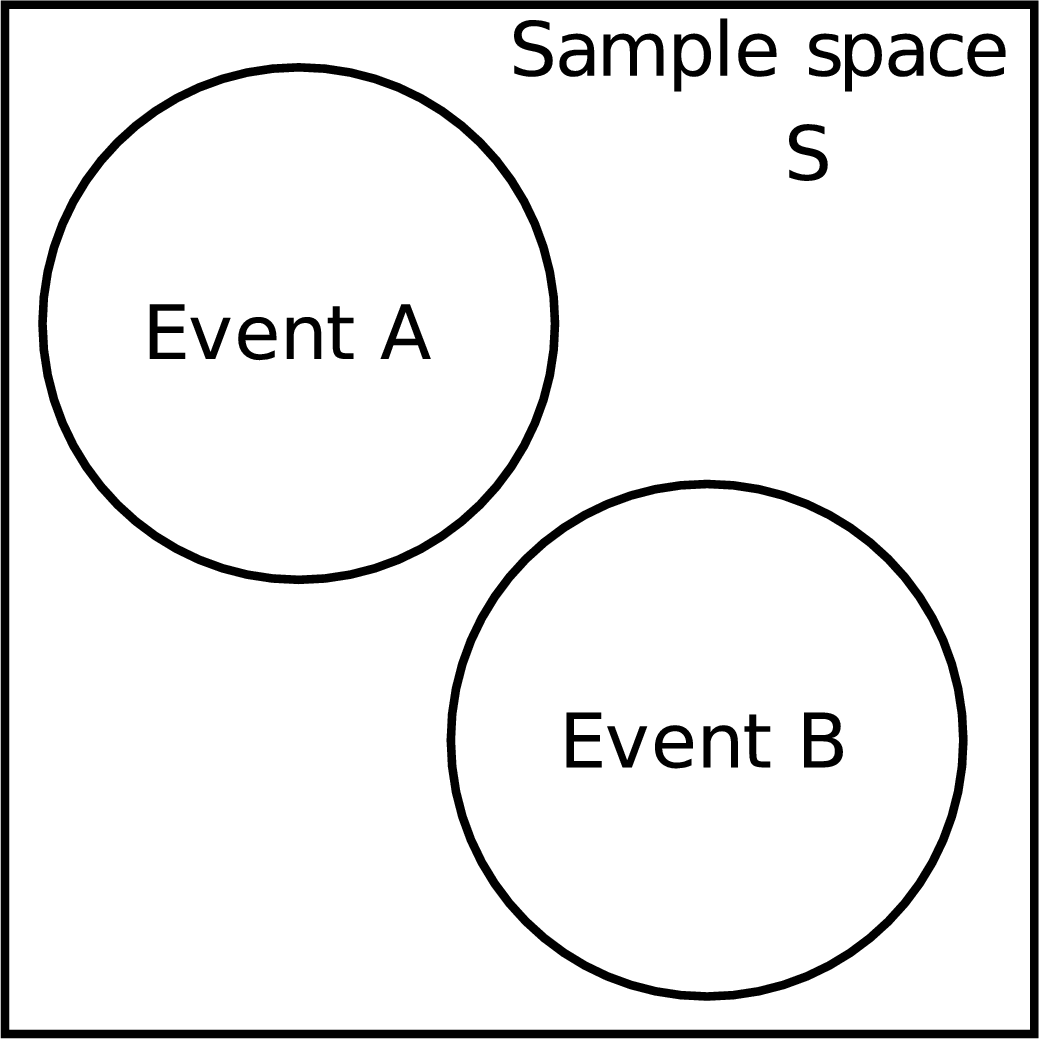
\includegraphics[width=200px]{col11306.imgs/m39377_mutualexclusive.png} % m39377;mutualexclusive.png;;;6.0;8.5;
        
      \vspace{2pt}
    \vspace{\rubberspace}\par \begin{cnxcaption}
	  \small \textbf{Figure 11.14: }Venn diagram for mutually exclusive events
	\end{cnxcaption}
      
    \vspace{.1in}
    
    \end{center}

 \end{figure}   

    \addtocounter{footnote}{-0}
    
\par \label{m39377*secfhsst!!!underscore!!!id1048}
            \subsection{Exercise: Mutually Exclusive Events }
            \nopagebreak
            \label{m39377*id114930}\begin{enumerate}[noitemsep, label=\textbf{\arabic*}. ] 
            \label{m39377*uid79}\item A box contains coloured blocks. The number of each colour is given in
the following table.

    % \textbf{m39377*id114946}\par
    
    % how many colspecs?  5
          % name: cnx:colspec
            % colnum: 1
            % colwidth: 10*
            % latex-name: columna
            % colname: 
            % align/tgroup-align/default: //left
            % -------------------------
            % name: cnx:colspec
            % colnum: 2
            % colwidth: 10*
            % latex-name: columnb
            % colname: 
            % align/tgroup-align/default: //left
            % -------------------------
            % name: cnx:colspec
            % colnum: 3
            % colwidth: 10*
            % latex-name: columnc
            % colname: 
            % align/tgroup-align/default: //left
            % -------------------------
            % name: cnx:colspec
            % colnum: 4
            % colwidth: 10*
            % latex-name: columnd
            % colname: 
            % align/tgroup-align/default: //left
            % -------------------------
            % name: cnx:colspec
            % colnum: 5
            % colwidth: 10*
            % latex-name: columne
            % colname: 
            % align/tgroup-align/default: //left
            % -------------------------
      
    
    \setlength\mytablespace{10\tabcolsep}
    \addtolength\mytablespace{6\arrayrulewidth}
    \setlength\mytablewidth{\linewidth}
        
    
    \setlength\mytableroom{\mytablewidth}
    \addtolength\mytableroom{-\mytablespace}
    
    \setlength\myfixedwidth{0pt}
    \setlength\mystarwidth{\mytableroom}
        \addtolength\mystarwidth{-\myfixedwidth}
        \divide\mystarwidth 50
        
    
      % ----- Begin capturing width of table in LR mode woof
      \settowidth{\mytableboxwidth}{\begin{tabular}[t]{|l|l|l|l|l|}\hline
    % count in rowspan-info-nodeset: 5
    % align/colidx: left,1
    
    % rowcount: '0' | start: 'false' | colidx: '1'
    
        % Formatting a regular cell and recurring on the next sibling
        Colour &
      % align/colidx: left,2
    
    % rowcount: '0' | start: 'false' | colidx: '2'
    
        % Formatting a regular cell and recurring on the next sibling
        Purple &
      % align/colidx: left,3
    
    % rowcount: '0' | start: 'false' | colidx: '3'
    
        % Formatting a regular cell and recurring on the next sibling
        Orange &
      % align/colidx: left,4
    
    % rowcount: '0' | start: 'false' | colidx: '4'
    
        % Formatting a regular cell and recurring on the next sibling
        White &
      % align/colidx: left,5
    
    % rowcount: '0' | start: 'false' | colidx: '5'
    
        % Formatting a regular cell and recurring on the next sibling
        Pink% make-rowspan-placeholders
    % rowspan info: col1 '0' | 'false' | '' || col2 '0' | 'false' | '' || col3 '0' | 'false' | '' || col4 '0' | 'false' | '' || col5 '0' | 'false' | ''
     \tabularnewline\cline{1-1}\cline{2-2}\cline{3-3}\cline{4-4}\cline{5-5}
      %--------------------------------------------------------------------
    % align/colidx: left,1
    
    % rowcount: '0' | start: 'false' | colidx: '1'
    
        % Formatting a regular cell and recurring on the next sibling
        Number of
blocks &
      % align/colidx: left,2
    
    % rowcount: '0' | start: 'false' | colidx: '2'
    
        % Formatting a regular cell and recurring on the next sibling
        24 &
      % align/colidx: left,3
    
    % rowcount: '0' | start: 'false' | colidx: '3'
    
        % Formatting a regular cell and recurring on the next sibling
        32 &
      % align/colidx: left,4
    
    % rowcount: '0' | start: 'false' | colidx: '4'
    
        % Formatting a regular cell and recurring on the next sibling
        41 &
      % align/colidx: left,5
    
    % rowcount: '0' | start: 'false' | colidx: '5'
    
        % Formatting a regular cell and recurring on the next sibling
        19% make-rowspan-placeholders
    % rowspan info: col1 '0' | 'false' | '' || col2 '0' | 'false' | '' || col3 '0' | 'false' | '' || col4 '0' | 'false' | '' || col5 '0' | 'false' | ''
     \tabularnewline\cline{1-1}\cline{2-2}\cline{3-3}\cline{4-4}\cline{5-5}
      %--------------------------------------------------------------------
    \end{tabular}} % end mytableboxwidth set
      \addtocounter{footnote}{-0}
      
      % ----- End capturing width of table in LR mode
    
        % ----- LR or paragraph mode: must test
        % ----- Begin capturing height of table
        \settoheight{\mytableboxheight}{\begin{tabular}[t]{|l|l|l|l|l|}\hline
    % count in rowspan-info-nodeset: 5
    % align/colidx: left,1
    
    % rowcount: '0' | start: 'false' | colidx: '1'
    
        % Formatting a regular cell and recurring on the next sibling
        Colour &
      % align/colidx: left,2
    
    % rowcount: '0' | start: 'false' | colidx: '2'
    
        % Formatting a regular cell and recurring on the next sibling
        Purple &
      % align/colidx: left,3
    
    % rowcount: '0' | start: 'false' | colidx: '3'
    
        % Formatting a regular cell and recurring on the next sibling
        Orange &
      % align/colidx: left,4
    
    % rowcount: '0' | start: 'false' | colidx: '4'
    
        % Formatting a regular cell and recurring on the next sibling
        White &
      % align/colidx: left,5
    
    % rowcount: '0' | start: 'false' | colidx: '5'
    
        % Formatting a regular cell and recurring on the next sibling
        Pink% make-rowspan-placeholders
    % rowspan info: col1 '0' | 'false' | '' || col2 '0' | 'false' | '' || col3 '0' | 'false' | '' || col4 '0' | 'false' | '' || col5 '0' | 'false' | ''
     \tabularnewline\cline{1-1}\cline{2-2}\cline{3-3}\cline{4-4}\cline{5-5}
      %--------------------------------------------------------------------
    % align/colidx: left,1
    
    % rowcount: '0' | start: 'false' | colidx: '1'
    
        % Formatting a regular cell and recurring on the next sibling
        Number of
blocks &
      % align/colidx: left,2
    
    % rowcount: '0' | start: 'false' | colidx: '2'
    
        % Formatting a regular cell and recurring on the next sibling
        24 &
      % align/colidx: left,3
    
    % rowcount: '0' | start: 'false' | colidx: '3'
    
        % Formatting a regular cell and recurring on the next sibling
        32 &
      % align/colidx: left,4
    
    % rowcount: '0' | start: 'false' | colidx: '4'
    
        % Formatting a regular cell and recurring on the next sibling
        41 &
      % align/colidx: left,5
    
    % rowcount: '0' | start: 'false' | colidx: '5'
    
        % Formatting a regular cell and recurring on the next sibling
        19% make-rowspan-placeholders
    % rowspan info: col1 '0' | 'false' | '' || col2 '0' | 'false' | '' || col3 '0' | 'false' | '' || col4 '0' | 'false' | '' || col5 '0' | 'false' | ''
     \tabularnewline\cline{1-1}\cline{2-2}\cline{3-3}\cline{4-4}\cline{5-5}
      %--------------------------------------------------------------------
    \end{tabular}} % end mytableboxheight set
        \settodepth{\mytableboxdepth}{\begin{tabular}[t]{|l|l|l|l|l|}\hline
    % count in rowspan-info-nodeset: 5
    % align/colidx: left,1
    
    % rowcount: '0' | start: 'false' | colidx: '1'
    
        % Formatting a regular cell and recurring on the next sibling
        Colour &
      % align/colidx: left,2
    
    % rowcount: '0' | start: 'false' | colidx: '2'
    
        % Formatting a regular cell and recurring on the next sibling
        Purple &
      % align/colidx: left,3
    
    % rowcount: '0' | start: 'false' | colidx: '3'
    
        % Formatting a regular cell and recurring on the next sibling
        Orange &
      % align/colidx: left,4
    
    % rowcount: '0' | start: 'false' | colidx: '4'
    
        % Formatting a regular cell and recurring on the next sibling
        White &
      % align/colidx: left,5
    
    % rowcount: '0' | start: 'false' | colidx: '5'
    
        % Formatting a regular cell and recurring on the next sibling
        Pink% make-rowspan-placeholders
    % rowspan info: col1 '0' | 'false' | '' || col2 '0' | 'false' | '' || col3 '0' | 'false' | '' || col4 '0' | 'false' | '' || col5 '0' | 'false' | ''
     \tabularnewline\cline{1-1}\cline{2-2}\cline{3-3}\cline{4-4}\cline{5-5}
      %--------------------------------------------------------------------
    % align/colidx: left,1
    
    % rowcount: '0' | start: 'false' | colidx: '1'
    
        % Formatting a regular cell and recurring on the next sibling
        Number of
blocks &
      % align/colidx: left,2
    
    % rowcount: '0' | start: 'false' | colidx: '2'
    
        % Formatting a regular cell and recurring on the next sibling
        24 &
      % align/colidx: left,3
    
    % rowcount: '0' | start: 'false' | colidx: '3'
    
        % Formatting a regular cell and recurring on the next sibling
        32 &
      % align/colidx: left,4
    
    % rowcount: '0' | start: 'false' | colidx: '4'
    
        % Formatting a regular cell and recurring on the next sibling
        41 &
      % align/colidx: left,5
    
    % rowcount: '0' | start: 'false' | colidx: '5'
    
        % Formatting a regular cell and recurring on the next sibling
        19% make-rowspan-placeholders
    % rowspan info: col1 '0' | 'false' | '' || col2 '0' | 'false' | '' || col3 '0' | 'false' | '' || col4 '0' | 'false' | '' || col5 '0' | 'false' | ''
     \tabularnewline\cline{1-1}\cline{2-2}\cline{3-3}\cline{4-4}\cline{5-5}
      %--------------------------------------------------------------------
    \end{tabular}} % end mytableboxdepth set
        \addtolength{\mytableboxheight}{\mytableboxdepth}
        % ----- End capturing height of table
        \addtocounter{footnote}{-0}
        
        \ifthenelse{\mytableboxwidth<\textwidth}{% the table fits in LR mode
          \addtolength{\mytableboxwidth}{-\mytablespace}
          \typeout{textheight: \the\textheight}
          \typeout{mytableboxheight: \the\mytableboxheight}
          \typeout{textwidth: \the\textwidth}
          \typeout{mytableboxwidth: \the\mytableboxwidth}
          \ifthenelse{\mytableboxheight<\textheight}{%
        
    % \begin{table}[H]
    % \\ 'id2936502' '1'
    
        \begin{center}
      
      \label{m39377*id114946}
      
    \noindent
    \begin{tabular}[t]{|l|l|l|l|l|}\hline
    % count in rowspan-info-nodeset: 5
    % align/colidx: left,1
    
    % rowcount: '0' | start: 'false' | colidx: '1'
    
        % Formatting a regular cell and recurring on the next sibling
        Colour &
      % align/colidx: left,2
    
    % rowcount: '0' | start: 'false' | colidx: '2'
    
        % Formatting a regular cell and recurring on the next sibling
        Purple &
      % align/colidx: left,3
    
    % rowcount: '0' | start: 'false' | colidx: '3'
    
        % Formatting a regular cell and recurring on the next sibling
        Orange &
      % align/colidx: left,4
    
    % rowcount: '0' | start: 'false' | colidx: '4'
    
        % Formatting a regular cell and recurring on the next sibling
        White &
      % align/colidx: left,5
    
    % rowcount: '0' | start: 'false' | colidx: '5'
    
        % Formatting a regular cell and recurring on the next sibling
        Pink% make-rowspan-placeholders
    % rowspan info: col1 '0' | 'false' | '' || col2 '0' | 'false' | '' || col3 '0' | 'false' | '' || col4 '0' | 'false' | '' || col5 '0' | 'false' | ''
     \tabularnewline\cline{1-1}\cline{2-2}\cline{3-3}\cline{4-4}\cline{5-5}
      %--------------------------------------------------------------------
    % align/colidx: left,1
    
    % rowcount: '0' | start: 'false' | colidx: '1'
    
        % Formatting a regular cell and recurring on the next sibling
        Number of
blocks &
      % align/colidx: left,2
    
    % rowcount: '0' | start: 'false' | colidx: '2'
    
        % Formatting a regular cell and recurring on the next sibling
        24 &
      % align/colidx: left,3
    
    % rowcount: '0' | start: 'false' | colidx: '3'
    
        % Formatting a regular cell and recurring on the next sibling
        32 &
      % align/colidx: left,4
    
    % rowcount: '0' | start: 'false' | colidx: '4'
    
        % Formatting a regular cell and recurring on the next sibling
        41 &
      % align/colidx: left,5
    
    % rowcount: '0' | start: 'false' | colidx: '5'
    
        % Formatting a regular cell and recurring on the next sibling
        19% make-rowspan-placeholders
    % rowspan info: col1 '0' | 'false' | '' || col2 '0' | 'false' | '' || col3 '0' | 'false' | '' || col4 '0' | 'false' | '' || col5 '0' | 'false' | ''
     \tabularnewline\cline{1-1}\cline{2-2}\cline{3-3}\cline{4-4}\cline{5-5}
      %--------------------------------------------------------------------
    \end{tabular}
      \end{center}
    \begin{center}{\small\bfseries Table 11.1}\end{center}
    %\end{table}
    
    \addtocounter{footnote}{-0}
    
          }{ % else
        
    % \begin{table}[H]
    % \\ 'id2936502' '1'
    
        \begin{center}
      
      \label{m39377*id114946}
      
    \noindent
    \tabletail{%
        \hline
        \multicolumn{5}{|p{\mytableboxwidth}|}{\raggedleft \small \sl continued on next page}\\
        \hline
      }
      \tablelasttail{}
      \begin{xtabular}[t]{|l|l|l|l|l|}\hline
    % count in rowspan-info-nodeset: 5
    % align/colidx: left,1
    
    % rowcount: '0' | start: 'false' | colidx: '1'
    
        % Formatting a regular cell and recurring on the next sibling
        Colour &
      % align/colidx: left,2
    
    % rowcount: '0' | start: 'false' | colidx: '2'
    
        % Formatting a regular cell and recurring on the next sibling
        Purple &
      % align/colidx: left,3
    
    % rowcount: '0' | start: 'false' | colidx: '3'
    
        % Formatting a regular cell and recurring on the next sibling
        Orange &
      % align/colidx: left,4
    
    % rowcount: '0' | start: 'false' | colidx: '4'
    
        % Formatting a regular cell and recurring on the next sibling
        White &
      % align/colidx: left,5
    
    % rowcount: '0' | start: 'false' | colidx: '5'
    
        % Formatting a regular cell and recurring on the next sibling
        Pink% make-rowspan-placeholders
    % rowspan info: col1 '0' | 'false' | '' || col2 '0' | 'false' | '' || col3 '0' | 'false' | '' || col4 '0' | 'false' | '' || col5 '0' | 'false' | ''
     \tabularnewline\cline{1-1}\cline{2-2}\cline{3-3}\cline{4-4}\cline{5-5}
      %--------------------------------------------------------------------
    % align/colidx: left,1
    
    % rowcount: '0' | start: 'false' | colidx: '1'
    
        % Formatting a regular cell and recurring on the next sibling
        Number of
blocks &
      % align/colidx: left,2
    
    % rowcount: '0' | start: 'false' | colidx: '2'
    
        % Formatting a regular cell and recurring on the next sibling
        24 &
      % align/colidx: left,3
    
    % rowcount: '0' | start: 'false' | colidx: '3'
    
        % Formatting a regular cell and recurring on the next sibling
        32 &
      % align/colidx: left,4
    
    % rowcount: '0' | start: 'false' | colidx: '4'
    
        % Formatting a regular cell and recurring on the next sibling
        41 &
      % align/colidx: left,5
    
    % rowcount: '0' | start: 'false' | colidx: '5'
    
        % Formatting a regular cell and recurring on the next sibling
        19% make-rowspan-placeholders
    % rowspan info: col1 '0' | 'false' | '' || col2 '0' | 'false' | '' || col3 '0' | 'false' | '' || col4 '0' | 'false' | '' || col5 '0' | 'false' | ''
     \tabularnewline\cline{1-1}\cline{2-2}\cline{3-3}\cline{4-4}\cline{5-5}
      %--------------------------------------------------------------------
    \end{xtabular}
      \end{center}
    \begin{center}{\small\bfseries Table 11.1}\end{center}
    %\end{table}
    
    \addtocounter{footnote}{-0}
    
          } % 
        }{% else
        % typeset the table in paragraph mode
        % ----- Begin capturing height of table
        \settoheight{\mytableboxheight}{\begin{tabular*}{\mytablewidth}[t]{|p{10\mystarwidth}|p{10\mystarwidth}|p{10\mystarwidth}|p{10\mystarwidth}|p{10\mystarwidth}|}\hline
    % count in rowspan-info-nodeset: 5
    % align/colidx: left,1
    
    % rowcount: '0' | start: 'false' | colidx: '1'
    
        % Formatting a regular cell and recurring on the next sibling
        Colour &
      % align/colidx: left,2
    
    % rowcount: '0' | start: 'false' | colidx: '2'
    
        % Formatting a regular cell and recurring on the next sibling
        Purple &
      % align/colidx: left,3
    
    % rowcount: '0' | start: 'false' | colidx: '3'
    
        % Formatting a regular cell and recurring on the next sibling
        Orange &
      % align/colidx: left,4
    
    % rowcount: '0' | start: 'false' | colidx: '4'
    
        % Formatting a regular cell and recurring on the next sibling
        White &
      % align/colidx: left,5
    
    % rowcount: '0' | start: 'false' | colidx: '5'
    
        % Formatting a regular cell and recurring on the next sibling
        Pink% make-rowspan-placeholders
    % rowspan info: col1 '0' | 'false' | '' || col2 '0' | 'false' | '' || col3 '0' | 'false' | '' || col4 '0' | 'false' | '' || col5 '0' | 'false' | ''
     \tabularnewline\cline{1-1}\cline{2-2}\cline{3-3}\cline{4-4}\cline{5-5}
      %--------------------------------------------------------------------
    % align/colidx: left,1
    
    % rowcount: '0' | start: 'false' | colidx: '1'
    
        % Formatting a regular cell and recurring on the next sibling
        Number of
blocks &
      % align/colidx: left,2
    
    % rowcount: '0' | start: 'false' | colidx: '2'
    
        % Formatting a regular cell and recurring on the next sibling
        24 &
      % align/colidx: left,3
    
    % rowcount: '0' | start: 'false' | colidx: '3'
    
        % Formatting a regular cell and recurring on the next sibling
        32 &
      % align/colidx: left,4
    
    % rowcount: '0' | start: 'false' | colidx: '4'
    
        % Formatting a regular cell and recurring on the next sibling
        41 &
      % align/colidx: left,5
    
    % rowcount: '0' | start: 'false' | colidx: '5'
    
        % Formatting a regular cell and recurring on the next sibling
        19% make-rowspan-placeholders
    % rowspan info: col1 '0' | 'false' | '' || col2 '0' | 'false' | '' || col3 '0' | 'false' | '' || col4 '0' | 'false' | '' || col5 '0' | 'false' | ''
     \tabularnewline\cline{1-1}\cline{2-2}\cline{3-3}\cline{4-4}\cline{5-5}
      %--------------------------------------------------------------------
    \end{tabular*}} % end mytableboxheight set
        \settodepth{\mytableboxdepth}{\begin{tabular*}{\mytablewidth}[t]{|p{10\mystarwidth}|p{10\mystarwidth}|p{10\mystarwidth}|p{10\mystarwidth}|p{10\mystarwidth}|}\hline
    % count in rowspan-info-nodeset: 5
    % align/colidx: left,1
    
    % rowcount: '0' | start: 'false' | colidx: '1'
    
        % Formatting a regular cell and recurring on the next sibling
        Colour &
      % align/colidx: left,2
    
    % rowcount: '0' | start: 'false' | colidx: '2'
    
        % Formatting a regular cell and recurring on the next sibling
        Purple &
      % align/colidx: left,3
    
    % rowcount: '0' | start: 'false' | colidx: '3'
    
        % Formatting a regular cell and recurring on the next sibling
        Orange &
      % align/colidx: left,4
    
    % rowcount: '0' | start: 'false' | colidx: '4'
    
        % Formatting a regular cell and recurring on the next sibling
        White &
      % align/colidx: left,5
    
    % rowcount: '0' | start: 'false' | colidx: '5'
    
        % Formatting a regular cell and recurring on the next sibling
        Pink% make-rowspan-placeholders
    % rowspan info: col1 '0' | 'false' | '' || col2 '0' | 'false' | '' || col3 '0' | 'false' | '' || col4 '0' | 'false' | '' || col5 '0' | 'false' | ''
     \tabularnewline\cline{1-1}\cline{2-2}\cline{3-3}\cline{4-4}\cline{5-5}
      %--------------------------------------------------------------------
    % align/colidx: left,1
    
    % rowcount: '0' | start: 'false' | colidx: '1'
    
        % Formatting a regular cell and recurring on the next sibling
        Number of
blocks &
      % align/colidx: left,2
    
    % rowcount: '0' | start: 'false' | colidx: '2'
    
        % Formatting a regular cell and recurring on the next sibling
        24 &
      % align/colidx: left,3
    
    % rowcount: '0' | start: 'false' | colidx: '3'
    
        % Formatting a regular cell and recurring on the next sibling
        32 &
      % align/colidx: left,4
    
    % rowcount: '0' | start: 'false' | colidx: '4'
    
        % Formatting a regular cell and recurring on the next sibling
        41 &
      % align/colidx: left,5
    
    % rowcount: '0' | start: 'false' | colidx: '5'
    
        % Formatting a regular cell and recurring on the next sibling
        19% make-rowspan-placeholders
    % rowspan info: col1 '0' | 'false' | '' || col2 '0' | 'false' | '' || col3 '0' | 'false' | '' || col4 '0' | 'false' | '' || col5 '0' | 'false' | ''
     \tabularnewline\cline{1-1}\cline{2-2}\cline{3-3}\cline{4-4}\cline{5-5}
      %--------------------------------------------------------------------
    \end{tabular*}} % end mytableboxdepth set
        \addtolength{\mytableboxheight}{\mytableboxdepth}
        % ----- End capturing height of table
        \typeout{textheight: \the\textheight}
        \typeout{mytableboxheight: \the\mytableboxheight}
        \typeout{table too wide, outputting in para mode}
        
    % \begin{table}[H]
    % \\ 'id2936502' '1'
    
        \begin{center}
      
      \label{m39377*id114946}
      
    \noindent
    \tabletail{%
        \hline
        \multicolumn{5}{|p{\mytableroom}|}{\raggedleft \small \sl continued on next page}\\
        \hline
      }
      \tablelasttail{}
      \begin{xtabular*}{\mytablewidth}[t]{|p{10\mystarwidth}|p{10\mystarwidth}|p{10\mystarwidth}|p{10\mystarwidth}|p{10\mystarwidth}|}\hline
    % count in rowspan-info-nodeset: 5
    % align/colidx: left,1
    
    % rowcount: '0' | start: 'false' | colidx: '1'
    
        % Formatting a regular cell and recurring on the next sibling
        Colour &
      % align/colidx: left,2
    
    % rowcount: '0' | start: 'false' | colidx: '2'
    
        % Formatting a regular cell and recurring on the next sibling
        Purple &
      % align/colidx: left,3
    
    % rowcount: '0' | start: 'false' | colidx: '3'
    
        % Formatting a regular cell and recurring on the next sibling
        Orange &
      % align/colidx: left,4
    
    % rowcount: '0' | start: 'false' | colidx: '4'
    
        % Formatting a regular cell and recurring on the next sibling
        White &
      % align/colidx: left,5
    
    % rowcount: '0' | start: 'false' | colidx: '5'
    
        % Formatting a regular cell and recurring on the next sibling
        Pink% make-rowspan-placeholders
    % rowspan info: col1 '0' | 'false' | '' || col2 '0' | 'false' | '' || col3 '0' | 'false' | '' || col4 '0' | 'false' | '' || col5 '0' | 'false' | ''
     \tabularnewline\cline{1-1}\cline{2-2}\cline{3-3}\cline{4-4}\cline{5-5}
      %--------------------------------------------------------------------
    % align/colidx: left,1
    
    % rowcount: '0' | start: 'false' | colidx: '1'
    
        % Formatting a regular cell and recurring on the next sibling
        Number of
blocks &
      % align/colidx: left,2
    
    % rowcount: '0' | start: 'false' | colidx: '2'
    
        % Formatting a regular cell and recurring on the next sibling
        24 &
      % align/colidx: left,3
    
    % rowcount: '0' | start: 'false' | colidx: '3'
    
        % Formatting a regular cell and recurring on the next sibling
        32 &
      % align/colidx: left,4
    
    % rowcount: '0' | start: 'false' | colidx: '4'
    
        % Formatting a regular cell and recurring on the next sibling
        41 &
      % align/colidx: left,5
    
    % rowcount: '0' | start: 'false' | colidx: '5'
    
        % Formatting a regular cell and recurring on the next sibling
        19% make-rowspan-placeholders
    % rowspan info: col1 '0' | 'false' | '' || col2 '0' | 'false' | '' || col3 '0' | 'false' | '' || col4 '0' | 'false' | '' || col5 '0' | 'false' | ''
     \tabularnewline\cline{1-1}\cline{2-2}\cline{3-3}\cline{4-4}\cline{5-5}
      %--------------------------------------------------------------------
    \end{xtabular*}
      \end{center}
    \begin{center}{\small\bfseries Table 11.1}\end{center}
    %\end{table}
    
    \addtocounter{footnote}{-0}
    
        }% ending lr/para test clause
      
    \par
  
A block is selected randomly. What is the probability that the block will be:
\label{m39377*id115050}\begin{enumerate}[noitemsep, label=\textbf{\alph*}. ] 
            \label{m39377*uid80}\item purple
\label{m39377*uid81}\item purple or white
\label{m39377*uid82}\item pink and orange
\label{m39377*uid83}\item not orange?
\end{enumerate}
                \label{m39377*uid84}\item A small private school has a class with children of
various ages. The table gies the number of pupils of each age in the class.

    % \textbf{m39377*id115116}\par
    
    % how many colspecs?  6
          % name: cnx:colspec
            % colnum: 1
            % colwidth: 10*
            % latex-name: columna
            % colname: 
            % align/tgroup-align/default: //left
            % -------------------------
            % name: cnx:colspec
            % colnum: 2
            % colwidth: 10*
            % latex-name: columnb
            % colname: 
            % align/tgroup-align/default: //left
            % -------------------------
            % name: cnx:colspec
            % colnum: 3
            % colwidth: 10*
            % latex-name: columnc
            % colname: 
            % align/tgroup-align/default: //left
            % -------------------------
            % name: cnx:colspec
            % colnum: 4
            % colwidth: 10*
            % latex-name: columnd
            % colname: 
            % align/tgroup-align/default: //left
            % -------------------------
            % name: cnx:colspec
            % colnum: 5
            % colwidth: 10*
            % latex-name: columne
            % colname: 
            % align/tgroup-align/default: //left
            % -------------------------
            % name: cnx:colspec
            % colnum: 6
            % colwidth: 10*
            % latex-name: columnf
            % colname: 
            % align/tgroup-align/default: //left
            % -------------------------
      
    
    \setlength\mytablespace{12\tabcolsep}
    \addtolength\mytablespace{7\arrayrulewidth}
    \setlength\mytablewidth{\linewidth}
        
    
    \setlength\mytableroom{\mytablewidth}
    \addtolength\mytableroom{-\mytablespace}
    
    \setlength\myfixedwidth{0pt}
    \setlength\mystarwidth{\mytableroom}
        \addtolength\mystarwidth{-\myfixedwidth}
        \divide\mystarwidth 60
        
    
      % ----- Begin capturing width of table in LR mode woof
      \settowidth{\mytableboxwidth}{\begin{tabular}[t]{|l|l|l|l|l|l|}\hline
    % count in rowspan-info-nodeset: 6
    % align/colidx: left,1
    
    % rowcount: '0' | start: 'false' | colidx: '1'
    
        % Formatting a regular cell and recurring on the next sibling
        3 years
female &
      % align/colidx: left,2
    
    % rowcount: '0' | start: 'false' | colidx: '2'
    
        % Formatting a regular cell and recurring on the next sibling
        3 years male &
      % align/colidx: left,3
    
    % rowcount: '0' | start: 'false' | colidx: '3'
    
        % Formatting a regular cell and recurring on the next sibling
        4 years female &
      % align/colidx: left,4
    
    % rowcount: '0' | start: 'false' | colidx: '4'
    
        % Formatting a regular cell and recurring on the next sibling
        4
years male &
      % align/colidx: left,5
    
    % rowcount: '0' | start: 'false' | colidx: '5'
    
        % Formatting a regular cell and recurring on the next sibling
        5 years female &
      % align/colidx: left,6
    
    % rowcount: '0' | start: 'false' | colidx: '6'
    
        % Formatting a regular cell and recurring on the next sibling
        5 years male% make-rowspan-placeholders
    % rowspan info: col1 '0' | 'false' | '' || col2 '0' | 'false' | '' || col3 '0' | 'false' | '' || col4 '0' | 'false' | '' || col5 '0' | 'false' | '' || col6 '0' | 'false' | ''
     \tabularnewline\cline{1-1}\cline{2-2}\cline{3-3}\cline{4-4}\cline{5-5}\cline{6-6}
      %--------------------------------------------------------------------
    % align/colidx: left,1
    
    % rowcount: '0' | start: 'false' | colidx: '1'
    
        % Formatting a regular cell and recurring on the next sibling
        6 &
      % align/colidx: left,2
    
    % rowcount: '0' | start: 'false' | colidx: '2'
    
        % Formatting a regular cell and recurring on the next sibling
        2 &
      % align/colidx: left,3
    
    % rowcount: '0' | start: 'false' | colidx: '3'
    
        % Formatting a regular cell and recurring on the next sibling
        5 &
      % align/colidx: left,4
    
    % rowcount: '0' | start: 'false' | colidx: '4'
    
        % Formatting a regular cell and recurring on the next sibling
        7 &
      % align/colidx: left,5
    
    % rowcount: '0' | start: 'false' | colidx: '5'
    
        % Formatting a regular cell and recurring on the next sibling
        4 &
      % align/colidx: left,6
    
    % rowcount: '0' | start: 'false' | colidx: '6'
    
        % Formatting a regular cell and recurring on the next sibling
        6% make-rowspan-placeholders
    % rowspan info: col1 '0' | 'false' | '' || col2 '0' | 'false' | '' || col3 '0' | 'false' | '' || col4 '0' | 'false' | '' || col5 '0' | 'false' | '' || col6 '0' | 'false' | ''
     \tabularnewline\cline{1-1}\cline{2-2}\cline{3-3}\cline{4-4}\cline{5-5}\cline{6-6}
      %--------------------------------------------------------------------
    \end{tabular}} % end mytableboxwidth set
      \addtocounter{footnote}{-0}
      
      % ----- End capturing width of table in LR mode
    
        % ----- LR or paragraph mode: must test
        % ----- Begin capturing height of table
        \settoheight{\mytableboxheight}{\begin{tabular}[t]{|l|l|l|l|l|l|}\hline
    % count in rowspan-info-nodeset: 6
    % align/colidx: left,1
    
    % rowcount: '0' | start: 'false' | colidx: '1'
    
        % Formatting a regular cell and recurring on the next sibling
        3 years
female &
      % align/colidx: left,2
    
    % rowcount: '0' | start: 'false' | colidx: '2'
    
        % Formatting a regular cell and recurring on the next sibling
        3 years male &
      % align/colidx: left,3
    
    % rowcount: '0' | start: 'false' | colidx: '3'
    
        % Formatting a regular cell and recurring on the next sibling
        4 years female &
      % align/colidx: left,4
    
    % rowcount: '0' | start: 'false' | colidx: '4'
    
        % Formatting a regular cell and recurring on the next sibling
        4
years male &
      % align/colidx: left,5
    
    % rowcount: '0' | start: 'false' | colidx: '5'
    
        % Formatting a regular cell and recurring on the next sibling
        5 years female &
      % align/colidx: left,6
    
    % rowcount: '0' | start: 'false' | colidx: '6'
    
        % Formatting a regular cell and recurring on the next sibling
        5 years male% make-rowspan-placeholders
    % rowspan info: col1 '0' | 'false' | '' || col2 '0' | 'false' | '' || col3 '0' | 'false' | '' || col4 '0' | 'false' | '' || col5 '0' | 'false' | '' || col6 '0' | 'false' | ''
     \tabularnewline\cline{1-1}\cline{2-2}\cline{3-3}\cline{4-4}\cline{5-5}\cline{6-6}
      %--------------------------------------------------------------------
    % align/colidx: left,1
    
    % rowcount: '0' | start: 'false' | colidx: '1'
    
        % Formatting a regular cell and recurring on the next sibling
        6 &
      % align/colidx: left,2
    
    % rowcount: '0' | start: 'false' | colidx: '2'
    
        % Formatting a regular cell and recurring on the next sibling
        2 &
      % align/colidx: left,3
    
    % rowcount: '0' | start: 'false' | colidx: '3'
    
        % Formatting a regular cell and recurring on the next sibling
        5 &
      % align/colidx: left,4
    
    % rowcount: '0' | start: 'false' | colidx: '4'
    
        % Formatting a regular cell and recurring on the next sibling
        7 &
      % align/colidx: left,5
    
    % rowcount: '0' | start: 'false' | colidx: '5'
    
        % Formatting a regular cell and recurring on the next sibling
        4 &
      % align/colidx: left,6
    
    % rowcount: '0' | start: 'false' | colidx: '6'
    
        % Formatting a regular cell and recurring on the next sibling
        6% make-rowspan-placeholders
    % rowspan info: col1 '0' | 'false' | '' || col2 '0' | 'false' | '' || col3 '0' | 'false' | '' || col4 '0' | 'false' | '' || col5 '0' | 'false' | '' || col6 '0' | 'false' | ''
     \tabularnewline\cline{1-1}\cline{2-2}\cline{3-3}\cline{4-4}\cline{5-5}\cline{6-6}
      %--------------------------------------------------------------------
    \end{tabular}} % end mytableboxheight set
        \settodepth{\mytableboxdepth}{\begin{tabular}[t]{|l|l|l|l|l|l|}\hline
    % count in rowspan-info-nodeset: 6
    % align/colidx: left,1
    
    % rowcount: '0' | start: 'false' | colidx: '1'
    
        % Formatting a regular cell and recurring on the next sibling
        3 years
female &
      % align/colidx: left,2
    
    % rowcount: '0' | start: 'false' | colidx: '2'
    
        % Formatting a regular cell and recurring on the next sibling
        3 years male &
      % align/colidx: left,3
    
    % rowcount: '0' | start: 'false' | colidx: '3'
    
        % Formatting a regular cell and recurring on the next sibling
        4 years female &
      % align/colidx: left,4
    
    % rowcount: '0' | start: 'false' | colidx: '4'
    
        % Formatting a regular cell and recurring on the next sibling
        4
years male &
      % align/colidx: left,5
    
    % rowcount: '0' | start: 'false' | colidx: '5'
    
        % Formatting a regular cell and recurring on the next sibling
        5 years female &
      % align/colidx: left,6
    
    % rowcount: '0' | start: 'false' | colidx: '6'
    
        % Formatting a regular cell and recurring on the next sibling
        5 years male% make-rowspan-placeholders
    % rowspan info: col1 '0' | 'false' | '' || col2 '0' | 'false' | '' || col3 '0' | 'false' | '' || col4 '0' | 'false' | '' || col5 '0' | 'false' | '' || col6 '0' | 'false' | ''
     \tabularnewline\cline{1-1}\cline{2-2}\cline{3-3}\cline{4-4}\cline{5-5}\cline{6-6}
      %--------------------------------------------------------------------
    % align/colidx: left,1
    
    % rowcount: '0' | start: 'false' | colidx: '1'
    
        % Formatting a regular cell and recurring on the next sibling
        6 &
      % align/colidx: left,2
    
    % rowcount: '0' | start: 'false' | colidx: '2'
    
        % Formatting a regular cell and recurring on the next sibling
        2 &
      % align/colidx: left,3
    
    % rowcount: '0' | start: 'false' | colidx: '3'
    
        % Formatting a regular cell and recurring on the next sibling
        5 &
      % align/colidx: left,4
    
    % rowcount: '0' | start: 'false' | colidx: '4'
    
        % Formatting a regular cell and recurring on the next sibling
        7 &
      % align/colidx: left,5
    
    % rowcount: '0' | start: 'false' | colidx: '5'
    
        % Formatting a regular cell and recurring on the next sibling
        4 &
      % align/colidx: left,6
    
    % rowcount: '0' | start: 'false' | colidx: '6'
    
        % Formatting a regular cell and recurring on the next sibling
        6% make-rowspan-placeholders
    % rowspan info: col1 '0' | 'false' | '' || col2 '0' | 'false' | '' || col3 '0' | 'false' | '' || col4 '0' | 'false' | '' || col5 '0' | 'false' | '' || col6 '0' | 'false' | ''
     \tabularnewline\cline{1-1}\cline{2-2}\cline{3-3}\cline{4-4}\cline{5-5}\cline{6-6}
      %--------------------------------------------------------------------
    \end{tabular}} % end mytableboxdepth set
        \addtolength{\mytableboxheight}{\mytableboxdepth}
        % ----- End capturing height of table
        \addtocounter{footnote}{-0}
        
        \ifthenelse{\mytableboxwidth<\textwidth}{% the table fits in LR mode
          \addtolength{\mytableboxwidth}{-\mytablespace}
          \typeout{textheight: \the\textheight}
          \typeout{mytableboxheight: \the\mytableboxheight}
          \typeout{textwidth: \the\textwidth}
          \typeout{mytableboxwidth: \the\mytableboxwidth}
          \ifthenelse{\mytableboxheight<\textheight}{%
        
    % \begin{table}[H]
    % \\ 'id2936592' '1'
    
        \begin{center}
      
      \label{m39377*id115116}
      
    \noindent
    \begin{tabular}[t]{|l|l|l|l|l|l|}\hline
    % count in rowspan-info-nodeset: 6
    % align/colidx: left,1
    
    % rowcount: '0' | start: 'false' | colidx: '1'
    
        % Formatting a regular cell and recurring on the next sibling
        3 years
female &
      % align/colidx: left,2
    
    % rowcount: '0' | start: 'false' | colidx: '2'
    
        % Formatting a regular cell and recurring on the next sibling
        3 years male &
      % align/colidx: left,3
    
    % rowcount: '0' | start: 'false' | colidx: '3'
    
        % Formatting a regular cell and recurring on the next sibling
        4 years female &
      % align/colidx: left,4
    
    % rowcount: '0' | start: 'false' | colidx: '4'
    
        % Formatting a regular cell and recurring on the next sibling
        4
years male &
      % align/colidx: left,5
    
    % rowcount: '0' | start: 'false' | colidx: '5'
    
        % Formatting a regular cell and recurring on the next sibling
        5 years female &
      % align/colidx: left,6
    
    % rowcount: '0' | start: 'false' | colidx: '6'
    
        % Formatting a regular cell and recurring on the next sibling
        5 years male% make-rowspan-placeholders
    % rowspan info: col1 '0' | 'false' | '' || col2 '0' | 'false' | '' || col3 '0' | 'false' | '' || col4 '0' | 'false' | '' || col5 '0' | 'false' | '' || col6 '0' | 'false' | ''
     \tabularnewline\cline{1-1}\cline{2-2}\cline{3-3}\cline{4-4}\cline{5-5}\cline{6-6}
      %--------------------------------------------------------------------
    % align/colidx: left,1
    
    % rowcount: '0' | start: 'false' | colidx: '1'
    
        % Formatting a regular cell and recurring on the next sibling
        6 &
      % align/colidx: left,2
    
    % rowcount: '0' | start: 'false' | colidx: '2'
    
        % Formatting a regular cell and recurring on the next sibling
        2 &
      % align/colidx: left,3
    
    % rowcount: '0' | start: 'false' | colidx: '3'
    
        % Formatting a regular cell and recurring on the next sibling
        5 &
      % align/colidx: left,4
    
    % rowcount: '0' | start: 'false' | colidx: '4'
    
        % Formatting a regular cell and recurring on the next sibling
        7 &
      % align/colidx: left,5
    
    % rowcount: '0' | start: 'false' | colidx: '5'
    
        % Formatting a regular cell and recurring on the next sibling
        4 &
      % align/colidx: left,6
    
    % rowcount: '0' | start: 'false' | colidx: '6'
    
        % Formatting a regular cell and recurring on the next sibling
        6% make-rowspan-placeholders
    % rowspan info: col1 '0' | 'false' | '' || col2 '0' | 'false' | '' || col3 '0' | 'false' | '' || col4 '0' | 'false' | '' || col5 '0' | 'false' | '' || col6 '0' | 'false' | ''
     \tabularnewline\cline{1-1}\cline{2-2}\cline{3-3}\cline{4-4}\cline{5-5}\cline{6-6}
      %--------------------------------------------------------------------
    \end{tabular}
      \end{center}
    \begin{center}{\small\bfseries Table 11.2}\end{center}
    %\end{table}
    
    \addtocounter{footnote}{-0}
    
          }{ % else
        
    % \begin{table}[H]
    % \\ 'id2936592' '1'
    
        \begin{center}
      
      \label{m39377*id115116}
      
    \noindent
    \tabletail{%
        \hline
        \multicolumn{6}{|p{\mytableboxwidth}|}{\raggedleft \small \sl continued on next page}\\
        \hline
      }
      \tablelasttail{}
      \begin{xtabular}[t]{|l|l|l|l|l|l|}\hline
    % count in rowspan-info-nodeset: 6
    % align/colidx: left,1
    
    % rowcount: '0' | start: 'false' | colidx: '1'
    
        % Formatting a regular cell and recurring on the next sibling
        3 years
female &
      % align/colidx: left,2
    
    % rowcount: '0' | start: 'false' | colidx: '2'
    
        % Formatting a regular cell and recurring on the next sibling
        3 years male &
      % align/colidx: left,3
    
    % rowcount: '0' | start: 'false' | colidx: '3'
    
        % Formatting a regular cell and recurring on the next sibling
        4 years female &
      % align/colidx: left,4
    
    % rowcount: '0' | start: 'false' | colidx: '4'
    
        % Formatting a regular cell and recurring on the next sibling
        4
years male &
      % align/colidx: left,5
    
    % rowcount: '0' | start: 'false' | colidx: '5'
    
        % Formatting a regular cell and recurring on the next sibling
        5 years female &
      % align/colidx: left,6
    
    % rowcount: '0' | start: 'false' | colidx: '6'
    
        % Formatting a regular cell and recurring on the next sibling
        5 years male% make-rowspan-placeholders
    % rowspan info: col1 '0' | 'false' | '' || col2 '0' | 'false' | '' || col3 '0' | 'false' | '' || col4 '0' | 'false' | '' || col5 '0' | 'false' | '' || col6 '0' | 'false' | ''
     \tabularnewline\cline{1-1}\cline{2-2}\cline{3-3}\cline{4-4}\cline{5-5}\cline{6-6}
      %--------------------------------------------------------------------
    % align/colidx: left,1
    
    % rowcount: '0' | start: 'false' | colidx: '1'
    
        % Formatting a regular cell and recurring on the next sibling
        6 &
      % align/colidx: left,2
    
    % rowcount: '0' | start: 'false' | colidx: '2'
    
        % Formatting a regular cell and recurring on the next sibling
        2 &
      % align/colidx: left,3
    
    % rowcount: '0' | start: 'false' | colidx: '3'
    
        % Formatting a regular cell and recurring on the next sibling
        5 &
      % align/colidx: left,4
    
    % rowcount: '0' | start: 'false' | colidx: '4'
    
        % Formatting a regular cell and recurring on the next sibling
        7 &
      % align/colidx: left,5
    
    % rowcount: '0' | start: 'false' | colidx: '5'
    
        % Formatting a regular cell and recurring on the next sibling
        4 &
      % align/colidx: left,6
    
    % rowcount: '0' | start: 'false' | colidx: '6'
    
        % Formatting a regular cell and recurring on the next sibling
        6% make-rowspan-placeholders
    % rowspan info: col1 '0' | 'false' | '' || col2 '0' | 'false' | '' || col3 '0' | 'false' | '' || col4 '0' | 'false' | '' || col5 '0' | 'false' | '' || col6 '0' | 'false' | ''
     \tabularnewline\cline{1-1}\cline{2-2}\cline{3-3}\cline{4-4}\cline{5-5}\cline{6-6}
      %--------------------------------------------------------------------
    \end{xtabular}
      \end{center}
    \begin{center}{\small\bfseries Table 11.2}\end{center}
    %\end{table}
    
    \addtocounter{footnote}{-0}
    
          } % 
        }{% else
        % typeset the table in paragraph mode
        % ----- Begin capturing height of table
        \settoheight{\mytableboxheight}{\begin{tabular*}{\mytablewidth}[t]{|p{10\mystarwidth}|p{10\mystarwidth}|p{10\mystarwidth}|p{10\mystarwidth}|p{10\mystarwidth}|p{10\mystarwidth}|}\hline
    % count in rowspan-info-nodeset: 6
    % align/colidx: left,1
    
    % rowcount: '0' | start: 'false' | colidx: '1'
    
        % Formatting a regular cell and recurring on the next sibling
        3 years
female &
      % align/colidx: left,2
    
    % rowcount: '0' | start: 'false' | colidx: '2'
    
        % Formatting a regular cell and recurring on the next sibling
        3 years male &
      % align/colidx: left,3
    
    % rowcount: '0' | start: 'false' | colidx: '3'
    
        % Formatting a regular cell and recurring on the next sibling
        4 years female &
      % align/colidx: left,4
    
    % rowcount: '0' | start: 'false' | colidx: '4'
    
        % Formatting a regular cell and recurring on the next sibling
        4
years male &
      % align/colidx: left,5
    
    % rowcount: '0' | start: 'false' | colidx: '5'
    
        % Formatting a regular cell and recurring on the next sibling
        5 years female &
      % align/colidx: left,6
    
    % rowcount: '0' | start: 'false' | colidx: '6'
    
        % Formatting a regular cell and recurring on the next sibling
        5 years male% make-rowspan-placeholders
    % rowspan info: col1 '0' | 'false' | '' || col2 '0' | 'false' | '' || col3 '0' | 'false' | '' || col4 '0' | 'false' | '' || col5 '0' | 'false' | '' || col6 '0' | 'false' | ''
     \tabularnewline\cline{1-1}\cline{2-2}\cline{3-3}\cline{4-4}\cline{5-5}\cline{6-6}
      %--------------------------------------------------------------------
    % align/colidx: left,1
    
    % rowcount: '0' | start: 'false' | colidx: '1'
    
        % Formatting a regular cell and recurring on the next sibling
        6 &
      % align/colidx: left,2
    
    % rowcount: '0' | start: 'false' | colidx: '2'
    
        % Formatting a regular cell and recurring on the next sibling
        2 &
      % align/colidx: left,3
    
    % rowcount: '0' | start: 'false' | colidx: '3'
    
        % Formatting a regular cell and recurring on the next sibling
        5 &
      % align/colidx: left,4
    
    % rowcount: '0' | start: 'false' | colidx: '4'
    
        % Formatting a regular cell and recurring on the next sibling
        7 &
      % align/colidx: left,5
    
    % rowcount: '0' | start: 'false' | colidx: '5'
    
        % Formatting a regular cell and recurring on the next sibling
        4 &
      % align/colidx: left,6
    
    % rowcount: '0' | start: 'false' | colidx: '6'
    
        % Formatting a regular cell and recurring on the next sibling
        6% make-rowspan-placeholders
    % rowspan info: col1 '0' | 'false' | '' || col2 '0' | 'false' | '' || col3 '0' | 'false' | '' || col4 '0' | 'false' | '' || col5 '0' | 'false' | '' || col6 '0' | 'false' | ''
     \tabularnewline\cline{1-1}\cline{2-2}\cline{3-3}\cline{4-4}\cline{5-5}\cline{6-6}
      %--------------------------------------------------------------------
    \end{tabular*}} % end mytableboxheight set
        \settodepth{\mytableboxdepth}{\begin{tabular*}{\mytablewidth}[t]{|p{10\mystarwidth}|p{10\mystarwidth}|p{10\mystarwidth}|p{10\mystarwidth}|p{10\mystarwidth}|p{10\mystarwidth}|}\hline
    % count in rowspan-info-nodeset: 6
    % align/colidx: left,1
    
    % rowcount: '0' | start: 'false' | colidx: '1'
    
        % Formatting a regular cell and recurring on the next sibling
        3 years
female &
      % align/colidx: left,2
    
    % rowcount: '0' | start: 'false' | colidx: '2'
    
        % Formatting a regular cell and recurring on the next sibling
        3 years male &
      % align/colidx: left,3
    
    % rowcount: '0' | start: 'false' | colidx: '3'
    
        % Formatting a regular cell and recurring on the next sibling
        4 years female &
      % align/colidx: left,4
    
    % rowcount: '0' | start: 'false' | colidx: '4'
    
        % Formatting a regular cell and recurring on the next sibling
        4
years male &
      % align/colidx: left,5
    
    % rowcount: '0' | start: 'false' | colidx: '5'
    
        % Formatting a regular cell and recurring on the next sibling
        5 years female &
      % align/colidx: left,6
    
    % rowcount: '0' | start: 'false' | colidx: '6'
    
        % Formatting a regular cell and recurring on the next sibling
        5 years male% make-rowspan-placeholders
    % rowspan info: col1 '0' | 'false' | '' || col2 '0' | 'false' | '' || col3 '0' | 'false' | '' || col4 '0' | 'false' | '' || col5 '0' | 'false' | '' || col6 '0' | 'false' | ''
     \tabularnewline\cline{1-1}\cline{2-2}\cline{3-3}\cline{4-4}\cline{5-5}\cline{6-6}
      %--------------------------------------------------------------------
    % align/colidx: left,1
    
    % rowcount: '0' | start: 'false' | colidx: '1'
    
        % Formatting a regular cell and recurring on the next sibling
        6 &
      % align/colidx: left,2
    
    % rowcount: '0' | start: 'false' | colidx: '2'
    
        % Formatting a regular cell and recurring on the next sibling
        2 &
      % align/colidx: left,3
    
    % rowcount: '0' | start: 'false' | colidx: '3'
    
        % Formatting a regular cell and recurring on the next sibling
        5 &
      % align/colidx: left,4
    
    % rowcount: '0' | start: 'false' | colidx: '4'
    
        % Formatting a regular cell and recurring on the next sibling
        7 &
      % align/colidx: left,5
    
    % rowcount: '0' | start: 'false' | colidx: '5'
    
        % Formatting a regular cell and recurring on the next sibling
        4 &
      % align/colidx: left,6
    
    % rowcount: '0' | start: 'false' | colidx: '6'
    
        % Formatting a regular cell and recurring on the next sibling
        6% make-rowspan-placeholders
    % rowspan info: col1 '0' | 'false' | '' || col2 '0' | 'false' | '' || col3 '0' | 'false' | '' || col4 '0' | 'false' | '' || col5 '0' | 'false' | '' || col6 '0' | 'false' | ''
     \tabularnewline\cline{1-1}\cline{2-2}\cline{3-3}\cline{4-4}\cline{5-5}\cline{6-6}
      %--------------------------------------------------------------------
    \end{tabular*}} % end mytableboxdepth set
        \addtolength{\mytableboxheight}{\mytableboxdepth}
        % ----- End capturing height of table
        \typeout{textheight: \the\textheight}
        \typeout{mytableboxheight: \the\mytableboxheight}
        \typeout{table too wide, outputting in para mode}
        
    % \begin{table}[H]
    % \\ 'id2936592' '1'
    
        \begin{center}
      
      \label{m39377*id115116}
      
    \noindent
    \tabletail{%
        \hline
        \multicolumn{6}{|p{\mytableroom}|}{\raggedleft \small \sl continued on next page}\\
        \hline
      }
      \tablelasttail{}
      \begin{xtabular*}{\mytablewidth}[t]{|p{10\mystarwidth}|p{10\mystarwidth}|p{10\mystarwidth}|p{10\mystarwidth}|p{10\mystarwidth}|p{10\mystarwidth}|}\hline
    % count in rowspan-info-nodeset: 6
    % align/colidx: left,1
    
    % rowcount: '0' | start: 'false' | colidx: '1'
    
        % Formatting a regular cell and recurring on the next sibling
        3 years
female &
      % align/colidx: left,2
    
    % rowcount: '0' | start: 'false' | colidx: '2'
    
        % Formatting a regular cell and recurring on the next sibling
        3 years male &
      % align/colidx: left,3
    
    % rowcount: '0' | start: 'false' | colidx: '3'
    
        % Formatting a regular cell and recurring on the next sibling
        4 years female &
      % align/colidx: left,4
    
    % rowcount: '0' | start: 'false' | colidx: '4'
    
        % Formatting a regular cell and recurring on the next sibling
        4
years male &
      % align/colidx: left,5
    
    % rowcount: '0' | start: 'false' | colidx: '5'
    
        % Formatting a regular cell and recurring on the next sibling
        5 years female &
      % align/colidx: left,6
    
    % rowcount: '0' | start: 'false' | colidx: '6'
    
        % Formatting a regular cell and recurring on the next sibling
        5 years male% make-rowspan-placeholders
    % rowspan info: col1 '0' | 'false' | '' || col2 '0' | 'false' | '' || col3 '0' | 'false' | '' || col4 '0' | 'false' | '' || col5 '0' | 'false' | '' || col6 '0' | 'false' | ''
     \tabularnewline\cline{1-1}\cline{2-2}\cline{3-3}\cline{4-4}\cline{5-5}\cline{6-6}
      %--------------------------------------------------------------------
    % align/colidx: left,1
    
    % rowcount: '0' | start: 'false' | colidx: '1'
    
        % Formatting a regular cell and recurring on the next sibling
        6 &
      % align/colidx: left,2
    
    % rowcount: '0' | start: 'false' | colidx: '2'
    
        % Formatting a regular cell and recurring on the next sibling
        2 &
      % align/colidx: left,3
    
    % rowcount: '0' | start: 'false' | colidx: '3'
    
        % Formatting a regular cell and recurring on the next sibling
        5 &
      % align/colidx: left,4
    
    % rowcount: '0' | start: 'false' | colidx: '4'
    
        % Formatting a regular cell and recurring on the next sibling
        7 &
      % align/colidx: left,5
    
    % rowcount: '0' | start: 'false' | colidx: '5'
    
        % Formatting a regular cell and recurring on the next sibling
        4 &
      % align/colidx: left,6
    
    % rowcount: '0' | start: 'false' | colidx: '6'
    
        % Formatting a regular cell and recurring on the next sibling
        6% make-rowspan-placeholders
    % rowspan info: col1 '0' | 'false' | '' || col2 '0' | 'false' | '' || col3 '0' | 'false' | '' || col4 '0' | 'false' | '' || col5 '0' | 'false' | '' || col6 '0' | 'false' | ''
     \tabularnewline\cline{1-1}\cline{2-2}\cline{3-3}\cline{4-4}\cline{5-5}\cline{6-6}
      %--------------------------------------------------------------------
    \end{xtabular*}
      \end{center}
    \begin{center}{\small\bfseries Table 11.2}\end{center}
    %\end{table}
    
    \addtocounter{footnote}{-0}
    
        }% ending lr/para test clause
      
    \par
  
If a pupil is selceted at random what is the probability that the pupil will be:
\label{m39377*id115236}\begin{enumerate}[noitemsep, label=\textbf{\alph*}. ] 
            \label{m39377*uid85}\item a female
\label{m39377*uid86}\item a 4 year old male
\label{m39377*uid87}\item aged 3 or 4
\label{m39377*uid88}\item aged 3 and 4
\label{m39377*uid89}\item not 5
\label{m39377*uid90}\item either 3 or female?
\end{enumerate}
                \label{m39377*uid91}\item Fiona has 85 labeled discs, which are numbered from 1
to 85. If a disc is selected at random what is the probability that the disc
number:
\label{m39377*id115326}\begin{enumerate}[noitemsep, label=\textbf{\alph*}. ] 
            \label{m39377*uid92}\item ends with 5
\label{m39377*uid93}\item can be multiplied by 3
\label{m39377*uid94}\item can be multiplied by 6
\label{m39377*uid95}\item is number 65
\label{m39377*uid96}\item is not a multiple of 5
\label{m39377*uid97}\item is a multiple of 4 or 3
\label{m39377*uid98}\item is a multiple of 2 and 6
\label{m39377*uid99}\item is number 1?
\end{enumerate}
                \end{enumerate}
        
    
    
\label{m39377*secfhsst!!!underscore!!!id264}
\par \raisebox{-5 pt}{
\includegraphics[width=0.5cm]{col11306.imgs/summary_www.png}} Find the answers with the shortcodes:
 \par \begin{tabular}[h]{cccccc}
 (1.) laB  &  (2.) laK  &  (3.) lak  & \end{tabular}



            \subsubsection{  Random Experiments }
            \nopagebreak
            
          \label{m39377*id111123}\begin{enumerate}[noitemsep, label=\textbf{\arabic*}. ] 
            \label{m39377*uid16}\item  Let \begin{math}S\end{math} denote the set of
whole numbers from 1 to 16,
\begin{math}X\end{math} denote the
set of even numbers from 1 to 16 and
\begin{math}Y\end{math} denote the
set of prime numbers from 1 to 16\label{m39377*id111223}\begin{enumerate}[noitemsep, label=\textbf{\alph*}. ] 
            \label{m39377*uid17}\item Draw a Venn
diagram accurately depicting \begin{math}S\end{math},
\begin{math}X\end{math} and \begin{math}Y\end{math}.
\label{m39377*uid18}\item Find \begin{math}n\left(S\right)\end{math}, \begin{math}n\left(X\right)\end{math}, \begin{math}n\left(Y\right)\end{math}, \begin{math}n\left(X\cup Y\right)\end{math}, \begin{math}n\left(X\cap Y\right)\end{math}.
\end{enumerate}
                \label{m39377*uid19}\item There are 79 Grade 10 learners at school. All of
these take either Maths, Geography or History. The number who take Geography is
41, those who take History is 36, and 30 take Maths. The number who take Maths
and History is 16; the number who take Geography and History is 6, and there are
8 who take Maths only and 16 who take only History.
\label{m39377*id111373}\begin{enumerate}[noitemsep, label=\textbf{\alph*}. ] 
            \label{m39377*uid20}\item Draw a Venn diagram to illustrate
all this information.
\label{m39377*uid21}\item How many learners take Maths and Geography but not
History?
\label{m39377*uid22}\item How many learners take Geography only?
\label{m39377*uid23}\item How many learners take all three subjects?
\end{enumerate}
                \label{m39377*uid24}\item Pieces of paper labelled with the numbers 1 to 12
are placed in a box and the box is shaken. One piece of paper is taken out and
then replaced.
\label{m39377*id111437}\begin{enumerate}[noitemsep, label=\textbf{\alph*}. ] 
            \label{m39377*uid25}\item What is the sample space, \begin{math}S\end{math}?
\label{m39377*uid26}\item Write down the set \begin{math}A\end{math}, representing the event of taking a
piece of paper labelled with a factor of 12.
\label{m39377*uid27}\item Write down the set \begin{math}B\end{math}, representing the event of taking a
piece of paper labelled with a prime number.
\label{m39377*uid28}\item Represent \begin{math}A\end{math}, \begin{math}B\end{math} and \begin{math}S\end{math} by means of a Venn diagram.
\label{m39377*uid29}\item Find
\label{m39377*id111546}\begin{enumerate}[noitemsep, label=\textbf{\roman*}. ] 
            \label{m39377*uid30}\item \begin{math}n\left(S\right)\end{math}\label{m39377*uid31}\item \begin{math}n\left(A\right)\end{math}\label{m39377*uid32}\item \begin{math}n\left(B\right)\end{math}\label{m39377*uid33}\item \begin{math}n\left(A\cap B\right)\end{math}\label{m39377*uid34}\item \begin{math}n\left(A\cup B\right)\end{math}\end{enumerate}
        \label{m39377*uid35}\item Is \begin{math}n\left(A\cup B\right)=n\left(A\right)+n\left(B\right)-n\left(A\cap B\right)\end{math}?
\end{enumerate}
                \end{enumerate}
        
          




  \label{m39377**end}
          
\par \raisebox{-5 pt}{
\includegraphics[width=0.5cm]{col11306.imgs/summary_www.png}} Find the answers with the shortcodes:
 \par \begin{tabular}[h]{cccccc}
 (1.) lqe  &  (2.) lqt  &  (3.) lqz  & \end{tabular}



%          \section{ Probability: Part 2}
%     \nopagebreak
%             \label{m39373} $ \hspace{-5pt}\begin{array}{cccccccccccc}   
\includegraphics[width=0.75cm]{col11306.imgs/summary_fullmarks.png} &   \end{array} $ \hspace{2 pt}\raisebox{-5 pt}{} {(section shortcode: MG10086 )} \par 
%     
%     
%     
%     
%     
    
  
    \label{m39373*cid5}
            \section{ Relative Frequency \textsl{vs.}
Probability}
            \nopagebreak
            
      
      \label{m39373*id112458}There are two approaches to determining the
probability associated with any particular event of a random experiment:\par 
      \label{m39373*id112462}\begin{enumerate}[noitemsep, label=\textbf{\arabic*}. ] 
            \label{m39373*uid54}\item determining the total number of possible outcomes and
calculating the probability of each outcome using the definition of probability
\label{m39373*uid55}\item performing the experiment and calculating the relative
frequency of each outcome
\end{enumerate}
        
      \label{m39373*id112492}\textsl{Relative
frequency} is defined as the number of times an event happens in a
statistical experiment divided by the number of trials conducted.\par 
      \label{m39373*id112501}It takes a very large number of trials before the
relative frequency of obtaining a head on a toss of a coin approaches the
probability of obtaining a head on a toss of a coin (in fact, if the probability of an event occurring is something other than 1, i.e. it is always true, or 0, i.e. it is never true, then probability is only absolutely accurate when an infinite number of trials is conducted). For example, the data in
Table 11.3 represent the outcomes of repeating 100 trials of a
statistical experiment 100 times, i.e. tossing a coin 100 times.\par 
      
    % \textbf{m39373*uid56}\par
    
    % how many colspecs?  10
          % name: cnx:colspec
            % colnum: 1
            % colwidth: 10*
            % latex-name: columna
            % colname: 
            % align/tgroup-align/default: //left
            % -------------------------
            % name: cnx:colspec
            % colnum: 2
            % colwidth: 10*
            % latex-name: columnb
            % colname: 
            % align/tgroup-align/default: //left
            % -------------------------
            % name: cnx:colspec
            % colnum: 3
            % colwidth: 10*
            % latex-name: columnc
            % colname: 
            % align/tgroup-align/default: //left
            % -------------------------
            % name: cnx:colspec
            % colnum: 4
            % colwidth: 10*
            % latex-name: columnd
            % colname: 
            % align/tgroup-align/default: //left
            % -------------------------
            % name: cnx:colspec
            % colnum: 5
            % colwidth: 10*
            % latex-name: columne
            % colname: 
            % align/tgroup-align/default: //left
            % -------------------------
            % name: cnx:colspec
            % colnum: 6
            % colwidth: 10*
            % latex-name: columnf
            % colname: 
            % align/tgroup-align/default: //left
            % -------------------------
            % name: cnx:colspec
            % colnum: 7
            % colwidth: 10*
            % latex-name: columng
            % colname: 
            % align/tgroup-align/default: //left
            % -------------------------
            % name: cnx:colspec
            % colnum: 8
            % colwidth: 10*
            % latex-name: columnh
            % colname: 
            % align/tgroup-align/default: //left
            % -------------------------
            % name: cnx:colspec
            % colnum: 9
            % colwidth: 10*
            % latex-name: columni
            % colname: 
            % align/tgroup-align/default: //left
            % -------------------------
            % name: cnx:colspec
            % colnum: 10
            % colwidth: 10*
            % latex-name: columnj
            % colname: 
            % align/tgroup-align/default: //left
            % -------------------------
      
    
    \setlength\mytablespace{20\tabcolsep}
    \addtolength\mytablespace{11\arrayrulewidth}
    \setlength\mytablewidth{\linewidth}
        
    
    \setlength\mytableroom{\mytablewidth}
    \addtolength\mytableroom{-\mytablespace}
    
    \setlength\myfixedwidth{0pt}
    \setlength\mystarwidth{\mytableroom}
        \addtolength\mystarwidth{-\myfixedwidth}
        \divide\mystarwidth 100
        
    
      % ----- Begin capturing width of table in LR mode woof
      \settowidth{\mytableboxwidth}{\begin{tabular}[t]{|l|l|l|l|l|l|l|l|l|l|}\hline
    % count in rowspan-info-nodeset: 10
    % align/colidx: left,1
    
    % rowcount: '0' | start: 'false' | colidx: '1'
    
        % Formatting a regular cell and recurring on the next sibling
        H &
      % align/colidx: left,2
    
    % rowcount: '0' | start: 'false' | colidx: '2'
    
        % Formatting a regular cell and recurring on the next sibling
        T &
      % align/colidx: left,3
    
    % rowcount: '0' | start: 'false' | colidx: '3'
    
        % Formatting a regular cell and recurring on the next sibling
        T &
      % align/colidx: left,4
    
    % rowcount: '0' | start: 'false' | colidx: '4'
    
        % Formatting a regular cell and recurring on the next sibling
        H &
      % align/colidx: left,5
    
    % rowcount: '0' | start: 'false' | colidx: '5'
    
        % Formatting a regular cell and recurring on the next sibling
        H &
      % align/colidx: left,6
    
    % rowcount: '0' | start: 'false' | colidx: '6'
    
        % Formatting a regular cell and recurring on the next sibling
        T &
      % align/colidx: left,7
    
    % rowcount: '0' | start: 'false' | colidx: '7'
    
        % Formatting a regular cell and recurring on the next sibling
        H &
      % align/colidx: left,8
    
    % rowcount: '0' | start: 'false' | colidx: '8'
    
        % Formatting a regular cell and recurring on the next sibling
        H &
      % align/colidx: left,9
    
    % rowcount: '0' | start: 'false' | colidx: '9'
    
        % Formatting a regular cell and recurring on the next sibling
        H &
      % align/colidx: left,10
    
    % rowcount: '0' | start: 'false' | colidx: '10'
    
        % Formatting a regular cell and recurring on the next sibling
        H% make-rowspan-placeholders
    % rowspan info: col1 '0' | 'false' | '' || col2 '0' | 'false' | '' || col3 '0' | 'false' | '' || col4 '0' | 'false' | '' || col5 '0' | 'false' | '' || col6 '0' | 'false' | '' || col7 '0' | 'false' | '' || col8 '0' | 'false' | '' || col9 '0' | 'false' | '' || col10 '0' | 'false' | ''
     \tabularnewline\cline{1-1}\cline{2-2}\cline{3-3}\cline{4-4}\cline{5-5}\cline{6-6}\cline{7-7}\cline{8-8}\cline{9-9}\cline{10-10}
      %--------------------------------------------------------------------
    % align/colidx: left,1
    
    % rowcount: '0' | start: 'false' | colidx: '1'
    
        % Formatting a regular cell and recurring on the next sibling
        H &
      % align/colidx: left,2
    
    % rowcount: '0' | start: 'false' | colidx: '2'
    
        % Formatting a regular cell and recurring on the next sibling
        H &
      % align/colidx: left,3
    
    % rowcount: '0' | start: 'false' | colidx: '3'
    
        % Formatting a regular cell and recurring on the next sibling
        H &
      % align/colidx: left,4
    
    % rowcount: '0' | start: 'false' | colidx: '4'
    
        % Formatting a regular cell and recurring on the next sibling
        H &
      % align/colidx: left,5
    
    % rowcount: '0' | start: 'false' | colidx: '5'
    
        % Formatting a regular cell and recurring on the next sibling
        T &
      % align/colidx: left,6
    
    % rowcount: '0' | start: 'false' | colidx: '6'
    
        % Formatting a regular cell and recurring on the next sibling
        H &
      % align/colidx: left,7
    
    % rowcount: '0' | start: 'false' | colidx: '7'
    
        % Formatting a regular cell and recurring on the next sibling
        H &
      % align/colidx: left,8
    
    % rowcount: '0' | start: 'false' | colidx: '8'
    
        % Formatting a regular cell and recurring on the next sibling
        T &
      % align/colidx: left,9
    
    % rowcount: '0' | start: 'false' | colidx: '9'
    
        % Formatting a regular cell and recurring on the next sibling
        T &
      % align/colidx: left,10
    
    % rowcount: '0' | start: 'false' | colidx: '10'
    
        % Formatting a regular cell and recurring on the next sibling
        T% make-rowspan-placeholders
    % rowspan info: col1 '0' | 'false' | '' || col2 '0' | 'false' | '' || col3 '0' | 'false' | '' || col4 '0' | 'false' | '' || col5 '0' | 'false' | '' || col6 '0' | 'false' | '' || col7 '0' | 'false' | '' || col8 '0' | 'false' | '' || col9 '0' | 'false' | '' || col10 '0' | 'false' | ''
     \tabularnewline\cline{1-1}\cline{2-2}\cline{3-3}\cline{4-4}\cline{5-5}\cline{6-6}\cline{7-7}\cline{8-8}\cline{9-9}\cline{10-10}
      %--------------------------------------------------------------------
    % align/colidx: left,1
    
    % rowcount: '0' | start: 'false' | colidx: '1'
    
        % Formatting a regular cell and recurring on the next sibling
        T &
      % align/colidx: left,2
    
    % rowcount: '0' | start: 'false' | colidx: '2'
    
        % Formatting a regular cell and recurring on the next sibling
        T &
      % align/colidx: left,3
    
    % rowcount: '0' | start: 'false' | colidx: '3'
    
        % Formatting a regular cell and recurring on the next sibling
        H &
      % align/colidx: left,4
    
    % rowcount: '0' | start: 'false' | colidx: '4'
    
        % Formatting a regular cell and recurring on the next sibling
        T &
      % align/colidx: left,5
    
    % rowcount: '0' | start: 'false' | colidx: '5'
    
        % Formatting a regular cell and recurring on the next sibling
        T &
      % align/colidx: left,6
    
    % rowcount: '0' | start: 'false' | colidx: '6'
    
        % Formatting a regular cell and recurring on the next sibling
        H &
      % align/colidx: left,7
    
    % rowcount: '0' | start: 'false' | colidx: '7'
    
        % Formatting a regular cell and recurring on the next sibling
        T &
      % align/colidx: left,8
    
    % rowcount: '0' | start: 'false' | colidx: '8'
    
        % Formatting a regular cell and recurring on the next sibling
        H &
      % align/colidx: left,9
    
    % rowcount: '0' | start: 'false' | colidx: '9'
    
        % Formatting a regular cell and recurring on the next sibling
        T &
      % align/colidx: left,10
    
    % rowcount: '0' | start: 'false' | colidx: '10'
    
        % Formatting a regular cell and recurring on the next sibling
        H% make-rowspan-placeholders
    % rowspan info: col1 '0' | 'false' | '' || col2 '0' | 'false' | '' || col3 '0' | 'false' | '' || col4 '0' | 'false' | '' || col5 '0' | 'false' | '' || col6 '0' | 'false' | '' || col7 '0' | 'false' | '' || col8 '0' | 'false' | '' || col9 '0' | 'false' | '' || col10 '0' | 'false' | ''
     \tabularnewline\cline{1-1}\cline{2-2}\cline{3-3}\cline{4-4}\cline{5-5}\cline{6-6}\cline{7-7}\cline{8-8}\cline{9-9}\cline{10-10}
      %--------------------------------------------------------------------
    % align/colidx: left,1
    
    % rowcount: '0' | start: 'false' | colidx: '1'
    
        % Formatting a regular cell and recurring on the next sibling
        H &
      % align/colidx: left,2
    
    % rowcount: '0' | start: 'false' | colidx: '2'
    
        % Formatting a regular cell and recurring on the next sibling
        H &
      % align/colidx: left,3
    
    % rowcount: '0' | start: 'false' | colidx: '3'
    
        % Formatting a regular cell and recurring on the next sibling
        T &
      % align/colidx: left,4
    
    % rowcount: '0' | start: 'false' | colidx: '4'
    
        % Formatting a regular cell and recurring on the next sibling
        T &
      % align/colidx: left,5
    
    % rowcount: '0' | start: 'false' | colidx: '5'
    
        % Formatting a regular cell and recurring on the next sibling
        H &
      % align/colidx: left,6
    
    % rowcount: '0' | start: 'false' | colidx: '6'
    
        % Formatting a regular cell and recurring on the next sibling
        T &
      % align/colidx: left,7
    
    % rowcount: '0' | start: 'false' | colidx: '7'
    
        % Formatting a regular cell and recurring on the next sibling
        T &
      % align/colidx: left,8
    
    % rowcount: '0' | start: 'false' | colidx: '8'
    
        % Formatting a regular cell and recurring on the next sibling
        H &
      % align/colidx: left,9
    
    % rowcount: '0' | start: 'false' | colidx: '9'
    
        % Formatting a regular cell and recurring on the next sibling
        T &
      % align/colidx: left,10
    
    % rowcount: '0' | start: 'false' | colidx: '10'
    
        % Formatting a regular cell and recurring on the next sibling
        T% make-rowspan-placeholders
    % rowspan info: col1 '0' | 'false' | '' || col2 '0' | 'false' | '' || col3 '0' | 'false' | '' || col4 '0' | 'false' | '' || col5 '0' | 'false' | '' || col6 '0' | 'false' | '' || col7 '0' | 'false' | '' || col8 '0' | 'false' | '' || col9 '0' | 'false' | '' || col10 '0' | 'false' | ''
     \tabularnewline\cline{1-1}\cline{2-2}\cline{3-3}\cline{4-4}\cline{5-5}\cline{6-6}\cline{7-7}\cline{8-8}\cline{9-9}\cline{10-10}
      %--------------------------------------------------------------------
    % align/colidx: left,1
    
    % rowcount: '0' | start: 'false' | colidx: '1'
    
        % Formatting a regular cell and recurring on the next sibling
        T &
      % align/colidx: left,2
    
    % rowcount: '0' | start: 'false' | colidx: '2'
    
        % Formatting a regular cell and recurring on the next sibling
        H &
      % align/colidx: left,3
    
    % rowcount: '0' | start: 'false' | colidx: '3'
    
        % Formatting a regular cell and recurring on the next sibling
        H &
      % align/colidx: left,4
    
    % rowcount: '0' | start: 'false' | colidx: '4'
    
        % Formatting a regular cell and recurring on the next sibling
        H &
      % align/colidx: left,5
    
    % rowcount: '0' | start: 'false' | colidx: '5'
    
        % Formatting a regular cell and recurring on the next sibling
        T &
      % align/colidx: left,6
    
    % rowcount: '0' | start: 'false' | colidx: '6'
    
        % Formatting a regular cell and recurring on the next sibling
        T &
      % align/colidx: left,7
    
    % rowcount: '0' | start: 'false' | colidx: '7'
    
        % Formatting a regular cell and recurring on the next sibling
        H &
      % align/colidx: left,8
    
    % rowcount: '0' | start: 'false' | colidx: '8'
    
        % Formatting a regular cell and recurring on the next sibling
        T &
      % align/colidx: left,9
    
    % rowcount: '0' | start: 'false' | colidx: '9'
    
        % Formatting a regular cell and recurring on the next sibling
        T &
      % align/colidx: left,10
    
    % rowcount: '0' | start: 'false' | colidx: '10'
    
        % Formatting a regular cell and recurring on the next sibling
        H% make-rowspan-placeholders
    % rowspan info: col1 '0' | 'false' | '' || col2 '0' | 'false' | '' || col3 '0' | 'false' | '' || col4 '0' | 'false' | '' || col5 '0' | 'false' | '' || col6 '0' | 'false' | '' || col7 '0' | 'false' | '' || col8 '0' | 'false' | '' || col9 '0' | 'false' | '' || col10 '0' | 'false' | ''
     \tabularnewline\cline{1-1}\cline{2-2}\cline{3-3}\cline{4-4}\cline{5-5}\cline{6-6}\cline{7-7}\cline{8-8}\cline{9-9}\cline{10-10}
      %--------------------------------------------------------------------
    % align/colidx: left,1
    
    % rowcount: '0' | start: 'false' | colidx: '1'
    
        % Formatting a regular cell and recurring on the next sibling
        H &
      % align/colidx: left,2
    
    % rowcount: '0' | start: 'false' | colidx: '2'
    
        % Formatting a regular cell and recurring on the next sibling
        T &
      % align/colidx: left,3
    
    % rowcount: '0' | start: 'false' | colidx: '3'
    
        % Formatting a regular cell and recurring on the next sibling
        T &
      % align/colidx: left,4
    
    % rowcount: '0' | start: 'false' | colidx: '4'
    
        % Formatting a regular cell and recurring on the next sibling
        T &
      % align/colidx: left,5
    
    % rowcount: '0' | start: 'false' | colidx: '5'
    
        % Formatting a regular cell and recurring on the next sibling
        T &
      % align/colidx: left,6
    
    % rowcount: '0' | start: 'false' | colidx: '6'
    
        % Formatting a regular cell and recurring on the next sibling
        H &
      % align/colidx: left,7
    
    % rowcount: '0' | start: 'false' | colidx: '7'
    
        % Formatting a regular cell and recurring on the next sibling
        T &
      % align/colidx: left,8
    
    % rowcount: '0' | start: 'false' | colidx: '8'
    
        % Formatting a regular cell and recurring on the next sibling
        T &
      % align/colidx: left,9
    
    % rowcount: '0' | start: 'false' | colidx: '9'
    
        % Formatting a regular cell and recurring on the next sibling
        H &
      % align/colidx: left,10
    
    % rowcount: '0' | start: 'false' | colidx: '10'
    
        % Formatting a regular cell and recurring on the next sibling
        H% make-rowspan-placeholders
    % rowspan info: col1 '0' | 'false' | '' || col2 '0' | 'false' | '' || col3 '0' | 'false' | '' || col4 '0' | 'false' | '' || col5 '0' | 'false' | '' || col6 '0' | 'false' | '' || col7 '0' | 'false' | '' || col8 '0' | 'false' | '' || col9 '0' | 'false' | '' || col10 '0' | 'false' | ''
     \tabularnewline\cline{1-1}\cline{2-2}\cline{3-3}\cline{4-4}\cline{5-5}\cline{6-6}\cline{7-7}\cline{8-8}\cline{9-9}\cline{10-10}
      %--------------------------------------------------------------------
    % align/colidx: left,1
    
    % rowcount: '0' | start: 'false' | colidx: '1'
    
        % Formatting a regular cell and recurring on the next sibling
        T &
      % align/colidx: left,2
    
    % rowcount: '0' | start: 'false' | colidx: '2'
    
        % Formatting a regular cell and recurring on the next sibling
        T &
      % align/colidx: left,3
    
    % rowcount: '0' | start: 'false' | colidx: '3'
    
        % Formatting a regular cell and recurring on the next sibling
        H &
      % align/colidx: left,4
    
    % rowcount: '0' | start: 'false' | colidx: '4'
    
        % Formatting a regular cell and recurring on the next sibling
        T &
      % align/colidx: left,5
    
    % rowcount: '0' | start: 'false' | colidx: '5'
    
        % Formatting a regular cell and recurring on the next sibling
        T &
      % align/colidx: left,6
    
    % rowcount: '0' | start: 'false' | colidx: '6'
    
        % Formatting a regular cell and recurring on the next sibling
        H &
      % align/colidx: left,7
    
    % rowcount: '0' | start: 'false' | colidx: '7'
    
        % Formatting a regular cell and recurring on the next sibling
        T &
      % align/colidx: left,8
    
    % rowcount: '0' | start: 'false' | colidx: '8'
    
        % Formatting a regular cell and recurring on the next sibling
        T &
      % align/colidx: left,9
    
    % rowcount: '0' | start: 'false' | colidx: '9'
    
        % Formatting a regular cell and recurring on the next sibling
        H &
      % align/colidx: left,10
    
    % rowcount: '0' | start: 'false' | colidx: '10'
    
        % Formatting a regular cell and recurring on the next sibling
        T% make-rowspan-placeholders
    % rowspan info: col1 '0' | 'false' | '' || col2 '0' | 'false' | '' || col3 '0' | 'false' | '' || col4 '0' | 'false' | '' || col5 '0' | 'false' | '' || col6 '0' | 'false' | '' || col7 '0' | 'false' | '' || col8 '0' | 'false' | '' || col9 '0' | 'false' | '' || col10 '0' | 'false' | ''
     \tabularnewline\cline{1-1}\cline{2-2}\cline{3-3}\cline{4-4}\cline{5-5}\cline{6-6}\cline{7-7}\cline{8-8}\cline{9-9}\cline{10-10}
      %--------------------------------------------------------------------
    % align/colidx: left,1
    
    % rowcount: '0' | start: 'false' | colidx: '1'
    
        % Formatting a regular cell and recurring on the next sibling
        H &
      % align/colidx: left,2
    
    % rowcount: '0' | start: 'false' | colidx: '2'
    
        % Formatting a regular cell and recurring on the next sibling
        T &
      % align/colidx: left,3
    
    % rowcount: '0' | start: 'false' | colidx: '3'
    
        % Formatting a regular cell and recurring on the next sibling
        T &
      % align/colidx: left,4
    
    % rowcount: '0' | start: 'false' | colidx: '4'
    
        % Formatting a regular cell and recurring on the next sibling
        H &
      % align/colidx: left,5
    
    % rowcount: '0' | start: 'false' | colidx: '5'
    
        % Formatting a regular cell and recurring on the next sibling
        T &
      % align/colidx: left,6
    
    % rowcount: '0' | start: 'false' | colidx: '6'
    
        % Formatting a regular cell and recurring on the next sibling
        T &
      % align/colidx: left,7
    
    % rowcount: '0' | start: 'false' | colidx: '7'
    
        % Formatting a regular cell and recurring on the next sibling
        T &
      % align/colidx: left,8
    
    % rowcount: '0' | start: 'false' | colidx: '8'
    
        % Formatting a regular cell and recurring on the next sibling
        T &
      % align/colidx: left,9
    
    % rowcount: '0' | start: 'false' | colidx: '9'
    
        % Formatting a regular cell and recurring on the next sibling
        H &
      % align/colidx: left,10
    
    % rowcount: '0' | start: 'false' | colidx: '10'
    
        % Formatting a regular cell and recurring on the next sibling
        T% make-rowspan-placeholders
    % rowspan info: col1 '0' | 'false' | '' || col2 '0' | 'false' | '' || col3 '0' | 'false' | '' || col4 '0' | 'false' | '' || col5 '0' | 'false' | '' || col6 '0' | 'false' | '' || col7 '0' | 'false' | '' || col8 '0' | 'false' | '' || col9 '0' | 'false' | '' || col10 '0' | 'false' | ''
     \tabularnewline\cline{1-1}\cline{2-2}\cline{3-3}\cline{4-4}\cline{5-5}\cline{6-6}\cline{7-7}\cline{8-8}\cline{9-9}\cline{10-10}
      %--------------------------------------------------------------------
    % align/colidx: left,1
    
    % rowcount: '0' | start: 'false' | colidx: '1'
    
        % Formatting a regular cell and recurring on the next sibling
        T &
      % align/colidx: left,2
    
    % rowcount: '0' | start: 'false' | colidx: '2'
    
        % Formatting a regular cell and recurring on the next sibling
        H &
      % align/colidx: left,3
    
    % rowcount: '0' | start: 'false' | colidx: '3'
    
        % Formatting a regular cell and recurring on the next sibling
        T &
      % align/colidx: left,4
    
    % rowcount: '0' | start: 'false' | colidx: '4'
    
        % Formatting a regular cell and recurring on the next sibling
        T &
      % align/colidx: left,5
    
    % rowcount: '0' | start: 'false' | colidx: '5'
    
        % Formatting a regular cell and recurring on the next sibling
        H &
      % align/colidx: left,6
    
    % rowcount: '0' | start: 'false' | colidx: '6'
    
        % Formatting a regular cell and recurring on the next sibling
        H &
      % align/colidx: left,7
    
    % rowcount: '0' | start: 'false' | colidx: '7'
    
        % Formatting a regular cell and recurring on the next sibling
        H &
      % align/colidx: left,8
    
    % rowcount: '0' | start: 'false' | colidx: '8'
    
        % Formatting a regular cell and recurring on the next sibling
        T &
      % align/colidx: left,9
    
    % rowcount: '0' | start: 'false' | colidx: '9'
    
        % Formatting a regular cell and recurring on the next sibling
        H &
      % align/colidx: left,10
    
    % rowcount: '0' | start: 'false' | colidx: '10'
    
        % Formatting a regular cell and recurring on the next sibling
        T% make-rowspan-placeholders
    % rowspan info: col1 '0' | 'false' | '' || col2 '0' | 'false' | '' || col3 '0' | 'false' | '' || col4 '0' | 'false' | '' || col5 '0' | 'false' | '' || col6 '0' | 'false' | '' || col7 '0' | 'false' | '' || col8 '0' | 'false' | '' || col9 '0' | 'false' | '' || col10 '0' | 'false' | ''
     \tabularnewline\cline{1-1}\cline{2-2}\cline{3-3}\cline{4-4}\cline{5-5}\cline{6-6}\cline{7-7}\cline{8-8}\cline{9-9}\cline{10-10}
      %--------------------------------------------------------------------
    % align/colidx: left,1
    
    % rowcount: '0' | start: 'false' | colidx: '1'
    
        % Formatting a regular cell and recurring on the next sibling
        T &
      % align/colidx: left,2
    
    % rowcount: '0' | start: 'false' | colidx: '2'
    
        % Formatting a regular cell and recurring on the next sibling
        T &
      % align/colidx: left,3
    
    % rowcount: '0' | start: 'false' | colidx: '3'
    
        % Formatting a regular cell and recurring on the next sibling
        T &
      % align/colidx: left,4
    
    % rowcount: '0' | start: 'false' | colidx: '4'
    
        % Formatting a regular cell and recurring on the next sibling
        H &
      % align/colidx: left,5
    
    % rowcount: '0' | start: 'false' | colidx: '5'
    
        % Formatting a regular cell and recurring on the next sibling
        H &
      % align/colidx: left,6
    
    % rowcount: '0' | start: 'false' | colidx: '6'
    
        % Formatting a regular cell and recurring on the next sibling
        T &
      % align/colidx: left,7
    
    % rowcount: '0' | start: 'false' | colidx: '7'
    
        % Formatting a regular cell and recurring on the next sibling
        T &
      % align/colidx: left,8
    
    % rowcount: '0' | start: 'false' | colidx: '8'
    
        % Formatting a regular cell and recurring on the next sibling
        T &
      % align/colidx: left,9
    
    % rowcount: '0' | start: 'false' | colidx: '9'
    
        % Formatting a regular cell and recurring on the next sibling
        H &
      % align/colidx: left,10
    
    % rowcount: '0' | start: 'false' | colidx: '10'
    
        % Formatting a regular cell and recurring on the next sibling
        T% make-rowspan-placeholders
    % rowspan info: col1 '0' | 'false' | '' || col2 '0' | 'false' | '' || col3 '0' | 'false' | '' || col4 '0' | 'false' | '' || col5 '0' | 'false' | '' || col6 '0' | 'false' | '' || col7 '0' | 'false' | '' || col8 '0' | 'false' | '' || col9 '0' | 'false' | '' || col10 '0' | 'false' | ''
     \tabularnewline\cline{1-1}\cline{2-2}\cline{3-3}\cline{4-4}\cline{5-5}\cline{6-6}\cline{7-7}\cline{8-8}\cline{9-9}\cline{10-10}
      %--------------------------------------------------------------------
    \end{tabular}} % end mytableboxwidth set
      \addtocounter{footnote}{-0}
      
      % ----- End capturing width of table in LR mode
    
        % ----- LR or paragraph mode: must test
        % ----- Begin capturing height of table
        \settoheight{\mytableboxheight}{\begin{tabular}[t]{|l|l|l|l|l|l|l|l|l|l|}\hline
    % count in rowspan-info-nodeset: 10
    % align/colidx: left,1
    
    % rowcount: '0' | start: 'false' | colidx: '1'
    
        % Formatting a regular cell and recurring on the next sibling
        H &
      % align/colidx: left,2
    
    % rowcount: '0' | start: 'false' | colidx: '2'
    
        % Formatting a regular cell and recurring on the next sibling
        T &
      % align/colidx: left,3
    
    % rowcount: '0' | start: 'false' | colidx: '3'
    
        % Formatting a regular cell and recurring on the next sibling
        T &
      % align/colidx: left,4
    
    % rowcount: '0' | start: 'false' | colidx: '4'
    
        % Formatting a regular cell and recurring on the next sibling
        H &
      % align/colidx: left,5
    
    % rowcount: '0' | start: 'false' | colidx: '5'
    
        % Formatting a regular cell and recurring on the next sibling
        H &
      % align/colidx: left,6
    
    % rowcount: '0' | start: 'false' | colidx: '6'
    
        % Formatting a regular cell and recurring on the next sibling
        T &
      % align/colidx: left,7
    
    % rowcount: '0' | start: 'false' | colidx: '7'
    
        % Formatting a regular cell and recurring on the next sibling
        H &
      % align/colidx: left,8
    
    % rowcount: '0' | start: 'false' | colidx: '8'
    
        % Formatting a regular cell and recurring on the next sibling
        H &
      % align/colidx: left,9
    
    % rowcount: '0' | start: 'false' | colidx: '9'
    
        % Formatting a regular cell and recurring on the next sibling
        H &
      % align/colidx: left,10
    
    % rowcount: '0' | start: 'false' | colidx: '10'
    
        % Formatting a regular cell and recurring on the next sibling
        H% make-rowspan-placeholders
    % rowspan info: col1 '0' | 'false' | '' || col2 '0' | 'false' | '' || col3 '0' | 'false' | '' || col4 '0' | 'false' | '' || col5 '0' | 'false' | '' || col6 '0' | 'false' | '' || col7 '0' | 'false' | '' || col8 '0' | 'false' | '' || col9 '0' | 'false' | '' || col10 '0' | 'false' | ''
     \tabularnewline\cline{1-1}\cline{2-2}\cline{3-3}\cline{4-4}\cline{5-5}\cline{6-6}\cline{7-7}\cline{8-8}\cline{9-9}\cline{10-10}
      %--------------------------------------------------------------------
    % align/colidx: left,1
    
    % rowcount: '0' | start: 'false' | colidx: '1'
    
        % Formatting a regular cell and recurring on the next sibling
        H &
      % align/colidx: left,2
    
    % rowcount: '0' | start: 'false' | colidx: '2'
    
        % Formatting a regular cell and recurring on the next sibling
        H &
      % align/colidx: left,3
    
    % rowcount: '0' | start: 'false' | colidx: '3'
    
        % Formatting a regular cell and recurring on the next sibling
        H &
      % align/colidx: left,4
    
    % rowcount: '0' | start: 'false' | colidx: '4'
    
        % Formatting a regular cell and recurring on the next sibling
        H &
      % align/colidx: left,5
    
    % rowcount: '0' | start: 'false' | colidx: '5'
    
        % Formatting a regular cell and recurring on the next sibling
        T &
      % align/colidx: left,6
    
    % rowcount: '0' | start: 'false' | colidx: '6'
    
        % Formatting a regular cell and recurring on the next sibling
        H &
      % align/colidx: left,7
    
    % rowcount: '0' | start: 'false' | colidx: '7'
    
        % Formatting a regular cell and recurring on the next sibling
        H &
      % align/colidx: left,8
    
    % rowcount: '0' | start: 'false' | colidx: '8'
    
        % Formatting a regular cell and recurring on the next sibling
        T &
      % align/colidx: left,9
    
    % rowcount: '0' | start: 'false' | colidx: '9'
    
        % Formatting a regular cell and recurring on the next sibling
        T &
      % align/colidx: left,10
    
    % rowcount: '0' | start: 'false' | colidx: '10'
    
        % Formatting a regular cell and recurring on the next sibling
        T% make-rowspan-placeholders
    % rowspan info: col1 '0' | 'false' | '' || col2 '0' | 'false' | '' || col3 '0' | 'false' | '' || col4 '0' | 'false' | '' || col5 '0' | 'false' | '' || col6 '0' | 'false' | '' || col7 '0' | 'false' | '' || col8 '0' | 'false' | '' || col9 '0' | 'false' | '' || col10 '0' | 'false' | ''
     \tabularnewline\cline{1-1}\cline{2-2}\cline{3-3}\cline{4-4}\cline{5-5}\cline{6-6}\cline{7-7}\cline{8-8}\cline{9-9}\cline{10-10}
      %--------------------------------------------------------------------
    % align/colidx: left,1
    
    % rowcount: '0' | start: 'false' | colidx: '1'
    
        % Formatting a regular cell and recurring on the next sibling
        T &
      % align/colidx: left,2
    
    % rowcount: '0' | start: 'false' | colidx: '2'
    
        % Formatting a regular cell and recurring on the next sibling
        T &
      % align/colidx: left,3
    
    % rowcount: '0' | start: 'false' | colidx: '3'
    
        % Formatting a regular cell and recurring on the next sibling
        H &
      % align/colidx: left,4
    
    % rowcount: '0' | start: 'false' | colidx: '4'
    
        % Formatting a regular cell and recurring on the next sibling
        T &
      % align/colidx: left,5
    
    % rowcount: '0' | start: 'false' | colidx: '5'
    
        % Formatting a regular cell and recurring on the next sibling
        T &
      % align/colidx: left,6
    
    % rowcount: '0' | start: 'false' | colidx: '6'
    
        % Formatting a regular cell and recurring on the next sibling
        H &
      % align/colidx: left,7
    
    % rowcount: '0' | start: 'false' | colidx: '7'
    
        % Formatting a regular cell and recurring on the next sibling
        T &
      % align/colidx: left,8
    
    % rowcount: '0' | start: 'false' | colidx: '8'
    
        % Formatting a regular cell and recurring on the next sibling
        H &
      % align/colidx: left,9
    
    % rowcount: '0' | start: 'false' | colidx: '9'
    
        % Formatting a regular cell and recurring on the next sibling
        T &
      % align/colidx: left,10
    
    % rowcount: '0' | start: 'false' | colidx: '10'
    
        % Formatting a regular cell and recurring on the next sibling
        H% make-rowspan-placeholders
    % rowspan info: col1 '0' | 'false' | '' || col2 '0' | 'false' | '' || col3 '0' | 'false' | '' || col4 '0' | 'false' | '' || col5 '0' | 'false' | '' || col6 '0' | 'false' | '' || col7 '0' | 'false' | '' || col8 '0' | 'false' | '' || col9 '0' | 'false' | '' || col10 '0' | 'false' | ''
     \tabularnewline\cline{1-1}\cline{2-2}\cline{3-3}\cline{4-4}\cline{5-5}\cline{6-6}\cline{7-7}\cline{8-8}\cline{9-9}\cline{10-10}
      %--------------------------------------------------------------------
    % align/colidx: left,1
    
    % rowcount: '0' | start: 'false' | colidx: '1'
    
        % Formatting a regular cell and recurring on the next sibling
        H &
      % align/colidx: left,2
    
    % rowcount: '0' | start: 'false' | colidx: '2'
    
        % Formatting a regular cell and recurring on the next sibling
        H &
      % align/colidx: left,3
    
    % rowcount: '0' | start: 'false' | colidx: '3'
    
        % Formatting a regular cell and recurring on the next sibling
        T &
      % align/colidx: left,4
    
    % rowcount: '0' | start: 'false' | colidx: '4'
    
        % Formatting a regular cell and recurring on the next sibling
        T &
      % align/colidx: left,5
    
    % rowcount: '0' | start: 'false' | colidx: '5'
    
        % Formatting a regular cell and recurring on the next sibling
        H &
      % align/colidx: left,6
    
    % rowcount: '0' | start: 'false' | colidx: '6'
    
        % Formatting a regular cell and recurring on the next sibling
        T &
      % align/colidx: left,7
    
    % rowcount: '0' | start: 'false' | colidx: '7'
    
        % Formatting a regular cell and recurring on the next sibling
        T &
      % align/colidx: left,8
    
    % rowcount: '0' | start: 'false' | colidx: '8'
    
        % Formatting a regular cell and recurring on the next sibling
        H &
      % align/colidx: left,9
    
    % rowcount: '0' | start: 'false' | colidx: '9'
    
        % Formatting a regular cell and recurring on the next sibling
        T &
      % align/colidx: left,10
    
    % rowcount: '0' | start: 'false' | colidx: '10'
    
        % Formatting a regular cell and recurring on the next sibling
        T% make-rowspan-placeholders
    % rowspan info: col1 '0' | 'false' | '' || col2 '0' | 'false' | '' || col3 '0' | 'false' | '' || col4 '0' | 'false' | '' || col5 '0' | 'false' | '' || col6 '0' | 'false' | '' || col7 '0' | 'false' | '' || col8 '0' | 'false' | '' || col9 '0' | 'false' | '' || col10 '0' | 'false' | ''
     \tabularnewline\cline{1-1}\cline{2-2}\cline{3-3}\cline{4-4}\cline{5-5}\cline{6-6}\cline{7-7}\cline{8-8}\cline{9-9}\cline{10-10}
      %--------------------------------------------------------------------
    % align/colidx: left,1
    
    % rowcount: '0' | start: 'false' | colidx: '1'
    
        % Formatting a regular cell and recurring on the next sibling
        T &
      % align/colidx: left,2
    
    % rowcount: '0' | start: 'false' | colidx: '2'
    
        % Formatting a regular cell and recurring on the next sibling
        H &
      % align/colidx: left,3
    
    % rowcount: '0' | start: 'false' | colidx: '3'
    
        % Formatting a regular cell and recurring on the next sibling
        H &
      % align/colidx: left,4
    
    % rowcount: '0' | start: 'false' | colidx: '4'
    
        % Formatting a regular cell and recurring on the next sibling
        H &
      % align/colidx: left,5
    
    % rowcount: '0' | start: 'false' | colidx: '5'
    
        % Formatting a regular cell and recurring on the next sibling
        T &
      % align/colidx: left,6
    
    % rowcount: '0' | start: 'false' | colidx: '6'
    
        % Formatting a regular cell and recurring on the next sibling
        T &
      % align/colidx: left,7
    
    % rowcount: '0' | start: 'false' | colidx: '7'
    
        % Formatting a regular cell and recurring on the next sibling
        H &
      % align/colidx: left,8
    
    % rowcount: '0' | start: 'false' | colidx: '8'
    
        % Formatting a regular cell and recurring on the next sibling
        T &
      % align/colidx: left,9
    
    % rowcount: '0' | start: 'false' | colidx: '9'
    
        % Formatting a regular cell and recurring on the next sibling
        T &
      % align/colidx: left,10
    
    % rowcount: '0' | start: 'false' | colidx: '10'
    
        % Formatting a regular cell and recurring on the next sibling
        H% make-rowspan-placeholders
    % rowspan info: col1 '0' | 'false' | '' || col2 '0' | 'false' | '' || col3 '0' | 'false' | '' || col4 '0' | 'false' | '' || col5 '0' | 'false' | '' || col6 '0' | 'false' | '' || col7 '0' | 'false' | '' || col8 '0' | 'false' | '' || col9 '0' | 'false' | '' || col10 '0' | 'false' | ''
     \tabularnewline\cline{1-1}\cline{2-2}\cline{3-3}\cline{4-4}\cline{5-5}\cline{6-6}\cline{7-7}\cline{8-8}\cline{9-9}\cline{10-10}
      %--------------------------------------------------------------------
    % align/colidx: left,1
    
    % rowcount: '0' | start: 'false' | colidx: '1'
    
        % Formatting a regular cell and recurring on the next sibling
        H &
      % align/colidx: left,2
    
    % rowcount: '0' | start: 'false' | colidx: '2'
    
        % Formatting a regular cell and recurring on the next sibling
        T &
      % align/colidx: left,3
    
    % rowcount: '0' | start: 'false' | colidx: '3'
    
        % Formatting a regular cell and recurring on the next sibling
        T &
      % align/colidx: left,4
    
    % rowcount: '0' | start: 'false' | colidx: '4'
    
        % Formatting a regular cell and recurring on the next sibling
        T &
      % align/colidx: left,5
    
    % rowcount: '0' | start: 'false' | colidx: '5'
    
        % Formatting a regular cell and recurring on the next sibling
        T &
      % align/colidx: left,6
    
    % rowcount: '0' | start: 'false' | colidx: '6'
    
        % Formatting a regular cell and recurring on the next sibling
        H &
      % align/colidx: left,7
    
    % rowcount: '0' | start: 'false' | colidx: '7'
    
        % Formatting a regular cell and recurring on the next sibling
        T &
      % align/colidx: left,8
    
    % rowcount: '0' | start: 'false' | colidx: '8'
    
        % Formatting a regular cell and recurring on the next sibling
        T &
      % align/colidx: left,9
    
    % rowcount: '0' | start: 'false' | colidx: '9'
    
        % Formatting a regular cell and recurring on the next sibling
        H &
      % align/colidx: left,10
    
    % rowcount: '0' | start: 'false' | colidx: '10'
    
        % Formatting a regular cell and recurring on the next sibling
        H% make-rowspan-placeholders
    % rowspan info: col1 '0' | 'false' | '' || col2 '0' | 'false' | '' || col3 '0' | 'false' | '' || col4 '0' | 'false' | '' || col5 '0' | 'false' | '' || col6 '0' | 'false' | '' || col7 '0' | 'false' | '' || col8 '0' | 'false' | '' || col9 '0' | 'false' | '' || col10 '0' | 'false' | ''
     \tabularnewline\cline{1-1}\cline{2-2}\cline{3-3}\cline{4-4}\cline{5-5}\cline{6-6}\cline{7-7}\cline{8-8}\cline{9-9}\cline{10-10}
      %--------------------------------------------------------------------
    % align/colidx: left,1
    
    % rowcount: '0' | start: 'false' | colidx: '1'
    
        % Formatting a regular cell and recurring on the next sibling
        T &
      % align/colidx: left,2
    
    % rowcount: '0' | start: 'false' | colidx: '2'
    
        % Formatting a regular cell and recurring on the next sibling
        T &
      % align/colidx: left,3
    
    % rowcount: '0' | start: 'false' | colidx: '3'
    
        % Formatting a regular cell and recurring on the next sibling
        H &
      % align/colidx: left,4
    
    % rowcount: '0' | start: 'false' | colidx: '4'
    
        % Formatting a regular cell and recurring on the next sibling
        T &
      % align/colidx: left,5
    
    % rowcount: '0' | start: 'false' | colidx: '5'
    
        % Formatting a regular cell and recurring on the next sibling
        T &
      % align/colidx: left,6
    
    % rowcount: '0' | start: 'false' | colidx: '6'
    
        % Formatting a regular cell and recurring on the next sibling
        H &
      % align/colidx: left,7
    
    % rowcount: '0' | start: 'false' | colidx: '7'
    
        % Formatting a regular cell and recurring on the next sibling
        T &
      % align/colidx: left,8
    
    % rowcount: '0' | start: 'false' | colidx: '8'
    
        % Formatting a regular cell and recurring on the next sibling
        T &
      % align/colidx: left,9
    
    % rowcount: '0' | start: 'false' | colidx: '9'
    
        % Formatting a regular cell and recurring on the next sibling
        H &
      % align/colidx: left,10
    
    % rowcount: '0' | start: 'false' | colidx: '10'
    
        % Formatting a regular cell and recurring on the next sibling
        T% make-rowspan-placeholders
    % rowspan info: col1 '0' | 'false' | '' || col2 '0' | 'false' | '' || col3 '0' | 'false' | '' || col4 '0' | 'false' | '' || col5 '0' | 'false' | '' || col6 '0' | 'false' | '' || col7 '0' | 'false' | '' || col8 '0' | 'false' | '' || col9 '0' | 'false' | '' || col10 '0' | 'false' | ''
     \tabularnewline\cline{1-1}\cline{2-2}\cline{3-3}\cline{4-4}\cline{5-5}\cline{6-6}\cline{7-7}\cline{8-8}\cline{9-9}\cline{10-10}
      %--------------------------------------------------------------------
    % align/colidx: left,1
    
    % rowcount: '0' | start: 'false' | colidx: '1'
    
        % Formatting a regular cell and recurring on the next sibling
        H &
      % align/colidx: left,2
    
    % rowcount: '0' | start: 'false' | colidx: '2'
    
        % Formatting a regular cell and recurring on the next sibling
        T &
      % align/colidx: left,3
    
    % rowcount: '0' | start: 'false' | colidx: '3'
    
        % Formatting a regular cell and recurring on the next sibling
        T &
      % align/colidx: left,4
    
    % rowcount: '0' | start: 'false' | colidx: '4'
    
        % Formatting a regular cell and recurring on the next sibling
        H &
      % align/colidx: left,5
    
    % rowcount: '0' | start: 'false' | colidx: '5'
    
        % Formatting a regular cell and recurring on the next sibling
        T &
      % align/colidx: left,6
    
    % rowcount: '0' | start: 'false' | colidx: '6'
    
        % Formatting a regular cell and recurring on the next sibling
        T &
      % align/colidx: left,7
    
    % rowcount: '0' | start: 'false' | colidx: '7'
    
        % Formatting a regular cell and recurring on the next sibling
        T &
      % align/colidx: left,8
    
    % rowcount: '0' | start: 'false' | colidx: '8'
    
        % Formatting a regular cell and recurring on the next sibling
        T &
      % align/colidx: left,9
    
    % rowcount: '0' | start: 'false' | colidx: '9'
    
        % Formatting a regular cell and recurring on the next sibling
        H &
      % align/colidx: left,10
    
    % rowcount: '0' | start: 'false' | colidx: '10'
    
        % Formatting a regular cell and recurring on the next sibling
        T% make-rowspan-placeholders
    % rowspan info: col1 '0' | 'false' | '' || col2 '0' | 'false' | '' || col3 '0' | 'false' | '' || col4 '0' | 'false' | '' || col5 '0' | 'false' | '' || col6 '0' | 'false' | '' || col7 '0' | 'false' | '' || col8 '0' | 'false' | '' || col9 '0' | 'false' | '' || col10 '0' | 'false' | ''
     \tabularnewline\cline{1-1}\cline{2-2}\cline{3-3}\cline{4-4}\cline{5-5}\cline{6-6}\cline{7-7}\cline{8-8}\cline{9-9}\cline{10-10}
      %--------------------------------------------------------------------
    % align/colidx: left,1
    
    % rowcount: '0' | start: 'false' | colidx: '1'
    
        % Formatting a regular cell and recurring on the next sibling
        T &
      % align/colidx: left,2
    
    % rowcount: '0' | start: 'false' | colidx: '2'
    
        % Formatting a regular cell and recurring on the next sibling
        H &
      % align/colidx: left,3
    
    % rowcount: '0' | start: 'false' | colidx: '3'
    
        % Formatting a regular cell and recurring on the next sibling
        T &
      % align/colidx: left,4
    
    % rowcount: '0' | start: 'false' | colidx: '4'
    
        % Formatting a regular cell and recurring on the next sibling
        T &
      % align/colidx: left,5
    
    % rowcount: '0' | start: 'false' | colidx: '5'
    
        % Formatting a regular cell and recurring on the next sibling
        H &
      % align/colidx: left,6
    
    % rowcount: '0' | start: 'false' | colidx: '6'
    
        % Formatting a regular cell and recurring on the next sibling
        H &
      % align/colidx: left,7
    
    % rowcount: '0' | start: 'false' | colidx: '7'
    
        % Formatting a regular cell and recurring on the next sibling
        H &
      % align/colidx: left,8
    
    % rowcount: '0' | start: 'false' | colidx: '8'
    
        % Formatting a regular cell and recurring on the next sibling
        T &
      % align/colidx: left,9
    
    % rowcount: '0' | start: 'false' | colidx: '9'
    
        % Formatting a regular cell and recurring on the next sibling
        H &
      % align/colidx: left,10
    
    % rowcount: '0' | start: 'false' | colidx: '10'
    
        % Formatting a regular cell and recurring on the next sibling
        T% make-rowspan-placeholders
    % rowspan info: col1 '0' | 'false' | '' || col2 '0' | 'false' | '' || col3 '0' | 'false' | '' || col4 '0' | 'false' | '' || col5 '0' | 'false' | '' || col6 '0' | 'false' | '' || col7 '0' | 'false' | '' || col8 '0' | 'false' | '' || col9 '0' | 'false' | '' || col10 '0' | 'false' | ''
     \tabularnewline\cline{1-1}\cline{2-2}\cline{3-3}\cline{4-4}\cline{5-5}\cline{6-6}\cline{7-7}\cline{8-8}\cline{9-9}\cline{10-10}
      %--------------------------------------------------------------------
    % align/colidx: left,1
    
    % rowcount: '0' | start: 'false' | colidx: '1'
    
        % Formatting a regular cell and recurring on the next sibling
        T &
      % align/colidx: left,2
    
    % rowcount: '0' | start: 'false' | colidx: '2'
    
        % Formatting a regular cell and recurring on the next sibling
        T &
      % align/colidx: left,3
    
    % rowcount: '0' | start: 'false' | colidx: '3'
    
        % Formatting a regular cell and recurring on the next sibling
        T &
      % align/colidx: left,4
    
    % rowcount: '0' | start: 'false' | colidx: '4'
    
        % Formatting a regular cell and recurring on the next sibling
        H &
      % align/colidx: left,5
    
    % rowcount: '0' | start: 'false' | colidx: '5'
    
        % Formatting a regular cell and recurring on the next sibling
        H &
      % align/colidx: left,6
    
    % rowcount: '0' | start: 'false' | colidx: '6'
    
        % Formatting a regular cell and recurring on the next sibling
        T &
      % align/colidx: left,7
    
    % rowcount: '0' | start: 'false' | colidx: '7'
    
        % Formatting a regular cell and recurring on the next sibling
        T &
      % align/colidx: left,8
    
    % rowcount: '0' | start: 'false' | colidx: '8'
    
        % Formatting a regular cell and recurring on the next sibling
        T &
      % align/colidx: left,9
    
    % rowcount: '0' | start: 'false' | colidx: '9'
    
        % Formatting a regular cell and recurring on the next sibling
        H &
      % align/colidx: left,10
    
    % rowcount: '0' | start: 'false' | colidx: '10'
    
        % Formatting a regular cell and recurring on the next sibling
        T% make-rowspan-placeholders
    % rowspan info: col1 '0' | 'false' | '' || col2 '0' | 'false' | '' || col3 '0' | 'false' | '' || col4 '0' | 'false' | '' || col5 '0' | 'false' | '' || col6 '0' | 'false' | '' || col7 '0' | 'false' | '' || col8 '0' | 'false' | '' || col9 '0' | 'false' | '' || col10 '0' | 'false' | ''
     \tabularnewline\cline{1-1}\cline{2-2}\cline{3-3}\cline{4-4}\cline{5-5}\cline{6-6}\cline{7-7}\cline{8-8}\cline{9-9}\cline{10-10}
      %--------------------------------------------------------------------
    \end{tabular}} % end mytableboxheight set
        \settodepth{\mytableboxdepth}{\begin{tabular}[t]{|l|l|l|l|l|l|l|l|l|l|}\hline
    % count in rowspan-info-nodeset: 10
    % align/colidx: left,1
    
    % rowcount: '0' | start: 'false' | colidx: '1'
    
        % Formatting a regular cell and recurring on the next sibling
        H &
      % align/colidx: left,2
    
    % rowcount: '0' | start: 'false' | colidx: '2'
    
        % Formatting a regular cell and recurring on the next sibling
        T &
      % align/colidx: left,3
    
    % rowcount: '0' | start: 'false' | colidx: '3'
    
        % Formatting a regular cell and recurring on the next sibling
        T &
      % align/colidx: left,4
    
    % rowcount: '0' | start: 'false' | colidx: '4'
    
        % Formatting a regular cell and recurring on the next sibling
        H &
      % align/colidx: left,5
    
    % rowcount: '0' | start: 'false' | colidx: '5'
    
        % Formatting a regular cell and recurring on the next sibling
        H &
      % align/colidx: left,6
    
    % rowcount: '0' | start: 'false' | colidx: '6'
    
        % Formatting a regular cell and recurring on the next sibling
        T &
      % align/colidx: left,7
    
    % rowcount: '0' | start: 'false' | colidx: '7'
    
        % Formatting a regular cell and recurring on the next sibling
        H &
      % align/colidx: left,8
    
    % rowcount: '0' | start: 'false' | colidx: '8'
    
        % Formatting a regular cell and recurring on the next sibling
        H &
      % align/colidx: left,9
    
    % rowcount: '0' | start: 'false' | colidx: '9'
    
        % Formatting a regular cell and recurring on the next sibling
        H &
      % align/colidx: left,10
    
    % rowcount: '0' | start: 'false' | colidx: '10'
    
        % Formatting a regular cell and recurring on the next sibling
        H% make-rowspan-placeholders
    % rowspan info: col1 '0' | 'false' | '' || col2 '0' | 'false' | '' || col3 '0' | 'false' | '' || col4 '0' | 'false' | '' || col5 '0' | 'false' | '' || col6 '0' | 'false' | '' || col7 '0' | 'false' | '' || col8 '0' | 'false' | '' || col9 '0' | 'false' | '' || col10 '0' | 'false' | ''
     \tabularnewline\cline{1-1}\cline{2-2}\cline{3-3}\cline{4-4}\cline{5-5}\cline{6-6}\cline{7-7}\cline{8-8}\cline{9-9}\cline{10-10}
      %--------------------------------------------------------------------
    % align/colidx: left,1
    
    % rowcount: '0' | start: 'false' | colidx: '1'
    
        % Formatting a regular cell and recurring on the next sibling
        H &
      % align/colidx: left,2
    
    % rowcount: '0' | start: 'false' | colidx: '2'
    
        % Formatting a regular cell and recurring on the next sibling
        H &
      % align/colidx: left,3
    
    % rowcount: '0' | start: 'false' | colidx: '3'
    
        % Formatting a regular cell and recurring on the next sibling
        H &
      % align/colidx: left,4
    
    % rowcount: '0' | start: 'false' | colidx: '4'
    
        % Formatting a regular cell and recurring on the next sibling
        H &
      % align/colidx: left,5
    
    % rowcount: '0' | start: 'false' | colidx: '5'
    
        % Formatting a regular cell and recurring on the next sibling
        T &
      % align/colidx: left,6
    
    % rowcount: '0' | start: 'false' | colidx: '6'
    
        % Formatting a regular cell and recurring on the next sibling
        H &
      % align/colidx: left,7
    
    % rowcount: '0' | start: 'false' | colidx: '7'
    
        % Formatting a regular cell and recurring on the next sibling
        H &
      % align/colidx: left,8
    
    % rowcount: '0' | start: 'false' | colidx: '8'
    
        % Formatting a regular cell and recurring on the next sibling
        T &
      % align/colidx: left,9
    
    % rowcount: '0' | start: 'false' | colidx: '9'
    
        % Formatting a regular cell and recurring on the next sibling
        T &
      % align/colidx: left,10
    
    % rowcount: '0' | start: 'false' | colidx: '10'
    
        % Formatting a regular cell and recurring on the next sibling
        T% make-rowspan-placeholders
    % rowspan info: col1 '0' | 'false' | '' || col2 '0' | 'false' | '' || col3 '0' | 'false' | '' || col4 '0' | 'false' | '' || col5 '0' | 'false' | '' || col6 '0' | 'false' | '' || col7 '0' | 'false' | '' || col8 '0' | 'false' | '' || col9 '0' | 'false' | '' || col10 '0' | 'false' | ''
     \tabularnewline\cline{1-1}\cline{2-2}\cline{3-3}\cline{4-4}\cline{5-5}\cline{6-6}\cline{7-7}\cline{8-8}\cline{9-9}\cline{10-10}
      %--------------------------------------------------------------------
    % align/colidx: left,1
    
    % rowcount: '0' | start: 'false' | colidx: '1'
    
        % Formatting a regular cell and recurring on the next sibling
        T &
      % align/colidx: left,2
    
    % rowcount: '0' | start: 'false' | colidx: '2'
    
        % Formatting a regular cell and recurring on the next sibling
        T &
      % align/colidx: left,3
    
    % rowcount: '0' | start: 'false' | colidx: '3'
    
        % Formatting a regular cell and recurring on the next sibling
        H &
      % align/colidx: left,4
    
    % rowcount: '0' | start: 'false' | colidx: '4'
    
        % Formatting a regular cell and recurring on the next sibling
        T &
      % align/colidx: left,5
    
    % rowcount: '0' | start: 'false' | colidx: '5'
    
        % Formatting a regular cell and recurring on the next sibling
        T &
      % align/colidx: left,6
    
    % rowcount: '0' | start: 'false' | colidx: '6'
    
        % Formatting a regular cell and recurring on the next sibling
        H &
      % align/colidx: left,7
    
    % rowcount: '0' | start: 'false' | colidx: '7'
    
        % Formatting a regular cell and recurring on the next sibling
        T &
      % align/colidx: left,8
    
    % rowcount: '0' | start: 'false' | colidx: '8'
    
        % Formatting a regular cell and recurring on the next sibling
        H &
      % align/colidx: left,9
    
    % rowcount: '0' | start: 'false' | colidx: '9'
    
        % Formatting a regular cell and recurring on the next sibling
        T &
      % align/colidx: left,10
    
    % rowcount: '0' | start: 'false' | colidx: '10'
    
        % Formatting a regular cell and recurring on the next sibling
        H% make-rowspan-placeholders
    % rowspan info: col1 '0' | 'false' | '' || col2 '0' | 'false' | '' || col3 '0' | 'false' | '' || col4 '0' | 'false' | '' || col5 '0' | 'false' | '' || col6 '0' | 'false' | '' || col7 '0' | 'false' | '' || col8 '0' | 'false' | '' || col9 '0' | 'false' | '' || col10 '0' | 'false' | ''
     \tabularnewline\cline{1-1}\cline{2-2}\cline{3-3}\cline{4-4}\cline{5-5}\cline{6-6}\cline{7-7}\cline{8-8}\cline{9-9}\cline{10-10}
      %--------------------------------------------------------------------
    % align/colidx: left,1
    
    % rowcount: '0' | start: 'false' | colidx: '1'
    
        % Formatting a regular cell and recurring on the next sibling
        H &
      % align/colidx: left,2
    
    % rowcount: '0' | start: 'false' | colidx: '2'
    
        % Formatting a regular cell and recurring on the next sibling
        H &
      % align/colidx: left,3
    
    % rowcount: '0' | start: 'false' | colidx: '3'
    
        % Formatting a regular cell and recurring on the next sibling
        T &
      % align/colidx: left,4
    
    % rowcount: '0' | start: 'false' | colidx: '4'
    
        % Formatting a regular cell and recurring on the next sibling
        T &
      % align/colidx: left,5
    
    % rowcount: '0' | start: 'false' | colidx: '5'
    
        % Formatting a regular cell and recurring on the next sibling
        H &
      % align/colidx: left,6
    
    % rowcount: '0' | start: 'false' | colidx: '6'
    
        % Formatting a regular cell and recurring on the next sibling
        T &
      % align/colidx: left,7
    
    % rowcount: '0' | start: 'false' | colidx: '7'
    
        % Formatting a regular cell and recurring on the next sibling
        T &
      % align/colidx: left,8
    
    % rowcount: '0' | start: 'false' | colidx: '8'
    
        % Formatting a regular cell and recurring on the next sibling
        H &
      % align/colidx: left,9
    
    % rowcount: '0' | start: 'false' | colidx: '9'
    
        % Formatting a regular cell and recurring on the next sibling
        T &
      % align/colidx: left,10
    
    % rowcount: '0' | start: 'false' | colidx: '10'
    
        % Formatting a regular cell and recurring on the next sibling
        T% make-rowspan-placeholders
    % rowspan info: col1 '0' | 'false' | '' || col2 '0' | 'false' | '' || col3 '0' | 'false' | '' || col4 '0' | 'false' | '' || col5 '0' | 'false' | '' || col6 '0' | 'false' | '' || col7 '0' | 'false' | '' || col8 '0' | 'false' | '' || col9 '0' | 'false' | '' || col10 '0' | 'false' | ''
     \tabularnewline\cline{1-1}\cline{2-2}\cline{3-3}\cline{4-4}\cline{5-5}\cline{6-6}\cline{7-7}\cline{8-8}\cline{9-9}\cline{10-10}
      %--------------------------------------------------------------------
    % align/colidx: left,1
    
    % rowcount: '0' | start: 'false' | colidx: '1'
    
        % Formatting a regular cell and recurring on the next sibling
        T &
      % align/colidx: left,2
    
    % rowcount: '0' | start: 'false' | colidx: '2'
    
        % Formatting a regular cell and recurring on the next sibling
        H &
      % align/colidx: left,3
    
    % rowcount: '0' | start: 'false' | colidx: '3'
    
        % Formatting a regular cell and recurring on the next sibling
        H &
      % align/colidx: left,4
    
    % rowcount: '0' | start: 'false' | colidx: '4'
    
        % Formatting a regular cell and recurring on the next sibling
        H &
      % align/colidx: left,5
    
    % rowcount: '0' | start: 'false' | colidx: '5'
    
        % Formatting a regular cell and recurring on the next sibling
        T &
      % align/colidx: left,6
    
    % rowcount: '0' | start: 'false' | colidx: '6'
    
        % Formatting a regular cell and recurring on the next sibling
        T &
      % align/colidx: left,7
    
    % rowcount: '0' | start: 'false' | colidx: '7'
    
        % Formatting a regular cell and recurring on the next sibling
        H &
      % align/colidx: left,8
    
    % rowcount: '0' | start: 'false' | colidx: '8'
    
        % Formatting a regular cell and recurring on the next sibling
        T &
      % align/colidx: left,9
    
    % rowcount: '0' | start: 'false' | colidx: '9'
    
        % Formatting a regular cell and recurring on the next sibling
        T &
      % align/colidx: left,10
    
    % rowcount: '0' | start: 'false' | colidx: '10'
    
        % Formatting a regular cell and recurring on the next sibling
        H% make-rowspan-placeholders
    % rowspan info: col1 '0' | 'false' | '' || col2 '0' | 'false' | '' || col3 '0' | 'false' | '' || col4 '0' | 'false' | '' || col5 '0' | 'false' | '' || col6 '0' | 'false' | '' || col7 '0' | 'false' | '' || col8 '0' | 'false' | '' || col9 '0' | 'false' | '' || col10 '0' | 'false' | ''
     \tabularnewline\cline{1-1}\cline{2-2}\cline{3-3}\cline{4-4}\cline{5-5}\cline{6-6}\cline{7-7}\cline{8-8}\cline{9-9}\cline{10-10}
      %--------------------------------------------------------------------
    % align/colidx: left,1
    
    % rowcount: '0' | start: 'false' | colidx: '1'
    
        % Formatting a regular cell and recurring on the next sibling
        H &
      % align/colidx: left,2
    
    % rowcount: '0' | start: 'false' | colidx: '2'
    
        % Formatting a regular cell and recurring on the next sibling
        T &
      % align/colidx: left,3
    
    % rowcount: '0' | start: 'false' | colidx: '3'
    
        % Formatting a regular cell and recurring on the next sibling
        T &
      % align/colidx: left,4
    
    % rowcount: '0' | start: 'false' | colidx: '4'
    
        % Formatting a regular cell and recurring on the next sibling
        T &
      % align/colidx: left,5
    
    % rowcount: '0' | start: 'false' | colidx: '5'
    
        % Formatting a regular cell and recurring on the next sibling
        T &
      % align/colidx: left,6
    
    % rowcount: '0' | start: 'false' | colidx: '6'
    
        % Formatting a regular cell and recurring on the next sibling
        H &
      % align/colidx: left,7
    
    % rowcount: '0' | start: 'false' | colidx: '7'
    
        % Formatting a regular cell and recurring on the next sibling
        T &
      % align/colidx: left,8
    
    % rowcount: '0' | start: 'false' | colidx: '8'
    
        % Formatting a regular cell and recurring on the next sibling
        T &
      % align/colidx: left,9
    
    % rowcount: '0' | start: 'false' | colidx: '9'
    
        % Formatting a regular cell and recurring on the next sibling
        H &
      % align/colidx: left,10
    
    % rowcount: '0' | start: 'false' | colidx: '10'
    
        % Formatting a regular cell and recurring on the next sibling
        H% make-rowspan-placeholders
    % rowspan info: col1 '0' | 'false' | '' || col2 '0' | 'false' | '' || col3 '0' | 'false' | '' || col4 '0' | 'false' | '' || col5 '0' | 'false' | '' || col6 '0' | 'false' | '' || col7 '0' | 'false' | '' || col8 '0' | 'false' | '' || col9 '0' | 'false' | '' || col10 '0' | 'false' | ''
     \tabularnewline\cline{1-1}\cline{2-2}\cline{3-3}\cline{4-4}\cline{5-5}\cline{6-6}\cline{7-7}\cline{8-8}\cline{9-9}\cline{10-10}
      %--------------------------------------------------------------------
    % align/colidx: left,1
    
    % rowcount: '0' | start: 'false' | colidx: '1'
    
        % Formatting a regular cell and recurring on the next sibling
        T &
      % align/colidx: left,2
    
    % rowcount: '0' | start: 'false' | colidx: '2'
    
        % Formatting a regular cell and recurring on the next sibling
        T &
      % align/colidx: left,3
    
    % rowcount: '0' | start: 'false' | colidx: '3'
    
        % Formatting a regular cell and recurring on the next sibling
        H &
      % align/colidx: left,4
    
    % rowcount: '0' | start: 'false' | colidx: '4'
    
        % Formatting a regular cell and recurring on the next sibling
        T &
      % align/colidx: left,5
    
    % rowcount: '0' | start: 'false' | colidx: '5'
    
        % Formatting a regular cell and recurring on the next sibling
        T &
      % align/colidx: left,6
    
    % rowcount: '0' | start: 'false' | colidx: '6'
    
        % Formatting a regular cell and recurring on the next sibling
        H &
      % align/colidx: left,7
    
    % rowcount: '0' | start: 'false' | colidx: '7'
    
        % Formatting a regular cell and recurring on the next sibling
        T &
      % align/colidx: left,8
    
    % rowcount: '0' | start: 'false' | colidx: '8'
    
        % Formatting a regular cell and recurring on the next sibling
        T &
      % align/colidx: left,9
    
    % rowcount: '0' | start: 'false' | colidx: '9'
    
        % Formatting a regular cell and recurring on the next sibling
        H &
      % align/colidx: left,10
    
    % rowcount: '0' | start: 'false' | colidx: '10'
    
        % Formatting a regular cell and recurring on the next sibling
        T% make-rowspan-placeholders
    % rowspan info: col1 '0' | 'false' | '' || col2 '0' | 'false' | '' || col3 '0' | 'false' | '' || col4 '0' | 'false' | '' || col5 '0' | 'false' | '' || col6 '0' | 'false' | '' || col7 '0' | 'false' | '' || col8 '0' | 'false' | '' || col9 '0' | 'false' | '' || col10 '0' | 'false' | ''
     \tabularnewline\cline{1-1}\cline{2-2}\cline{3-3}\cline{4-4}\cline{5-5}\cline{6-6}\cline{7-7}\cline{8-8}\cline{9-9}\cline{10-10}
      %--------------------------------------------------------------------
    % align/colidx: left,1
    
    % rowcount: '0' | start: 'false' | colidx: '1'
    
        % Formatting a regular cell and recurring on the next sibling
        H &
      % align/colidx: left,2
    
    % rowcount: '0' | start: 'false' | colidx: '2'
    
        % Formatting a regular cell and recurring on the next sibling
        T &
      % align/colidx: left,3
    
    % rowcount: '0' | start: 'false' | colidx: '3'
    
        % Formatting a regular cell and recurring on the next sibling
        T &
      % align/colidx: left,4
    
    % rowcount: '0' | start: 'false' | colidx: '4'
    
        % Formatting a regular cell and recurring on the next sibling
        H &
      % align/colidx: left,5
    
    % rowcount: '0' | start: 'false' | colidx: '5'
    
        % Formatting a regular cell and recurring on the next sibling
        T &
      % align/colidx: left,6
    
    % rowcount: '0' | start: 'false' | colidx: '6'
    
        % Formatting a regular cell and recurring on the next sibling
        T &
      % align/colidx: left,7
    
    % rowcount: '0' | start: 'false' | colidx: '7'
    
        % Formatting a regular cell and recurring on the next sibling
        T &
      % align/colidx: left,8
    
    % rowcount: '0' | start: 'false' | colidx: '8'
    
        % Formatting a regular cell and recurring on the next sibling
        T &
      % align/colidx: left,9
    
    % rowcount: '0' | start: 'false' | colidx: '9'
    
        % Formatting a regular cell and recurring on the next sibling
        H &
      % align/colidx: left,10
    
    % rowcount: '0' | start: 'false' | colidx: '10'
    
        % Formatting a regular cell and recurring on the next sibling
        T% make-rowspan-placeholders
    % rowspan info: col1 '0' | 'false' | '' || col2 '0' | 'false' | '' || col3 '0' | 'false' | '' || col4 '0' | 'false' | '' || col5 '0' | 'false' | '' || col6 '0' | 'false' | '' || col7 '0' | 'false' | '' || col8 '0' | 'false' | '' || col9 '0' | 'false' | '' || col10 '0' | 'false' | ''
     \tabularnewline\cline{1-1}\cline{2-2}\cline{3-3}\cline{4-4}\cline{5-5}\cline{6-6}\cline{7-7}\cline{8-8}\cline{9-9}\cline{10-10}
      %--------------------------------------------------------------------
    % align/colidx: left,1
    
    % rowcount: '0' | start: 'false' | colidx: '1'
    
        % Formatting a regular cell and recurring on the next sibling
        T &
      % align/colidx: left,2
    
    % rowcount: '0' | start: 'false' | colidx: '2'
    
        % Formatting a regular cell and recurring on the next sibling
        H &
      % align/colidx: left,3
    
    % rowcount: '0' | start: 'false' | colidx: '3'
    
        % Formatting a regular cell and recurring on the next sibling
        T &
      % align/colidx: left,4
    
    % rowcount: '0' | start: 'false' | colidx: '4'
    
        % Formatting a regular cell and recurring on the next sibling
        T &
      % align/colidx: left,5
    
    % rowcount: '0' | start: 'false' | colidx: '5'
    
        % Formatting a regular cell and recurring on the next sibling
        H &
      % align/colidx: left,6
    
    % rowcount: '0' | start: 'false' | colidx: '6'
    
        % Formatting a regular cell and recurring on the next sibling
        H &
      % align/colidx: left,7
    
    % rowcount: '0' | start: 'false' | colidx: '7'
    
        % Formatting a regular cell and recurring on the next sibling
        H &
      % align/colidx: left,8
    
    % rowcount: '0' | start: 'false' | colidx: '8'
    
        % Formatting a regular cell and recurring on the next sibling
        T &
      % align/colidx: left,9
    
    % rowcount: '0' | start: 'false' | colidx: '9'
    
        % Formatting a regular cell and recurring on the next sibling
        H &
      % align/colidx: left,10
    
    % rowcount: '0' | start: 'false' | colidx: '10'
    
        % Formatting a regular cell and recurring on the next sibling
        T% make-rowspan-placeholders
    % rowspan info: col1 '0' | 'false' | '' || col2 '0' | 'false' | '' || col3 '0' | 'false' | '' || col4 '0' | 'false' | '' || col5 '0' | 'false' | '' || col6 '0' | 'false' | '' || col7 '0' | 'false' | '' || col8 '0' | 'false' | '' || col9 '0' | 'false' | '' || col10 '0' | 'false' | ''
     \tabularnewline\cline{1-1}\cline{2-2}\cline{3-3}\cline{4-4}\cline{5-5}\cline{6-6}\cline{7-7}\cline{8-8}\cline{9-9}\cline{10-10}
      %--------------------------------------------------------------------
    % align/colidx: left,1
    
    % rowcount: '0' | start: 'false' | colidx: '1'
    
        % Formatting a regular cell and recurring on the next sibling
        T &
      % align/colidx: left,2
    
    % rowcount: '0' | start: 'false' | colidx: '2'
    
        % Formatting a regular cell and recurring on the next sibling
        T &
      % align/colidx: left,3
    
    % rowcount: '0' | start: 'false' | colidx: '3'
    
        % Formatting a regular cell and recurring on the next sibling
        T &
      % align/colidx: left,4
    
    % rowcount: '0' | start: 'false' | colidx: '4'
    
        % Formatting a regular cell and recurring on the next sibling
        H &
      % align/colidx: left,5
    
    % rowcount: '0' | start: 'false' | colidx: '5'
    
        % Formatting a regular cell and recurring on the next sibling
        H &
      % align/colidx: left,6
    
    % rowcount: '0' | start: 'false' | colidx: '6'
    
        % Formatting a regular cell and recurring on the next sibling
        T &
      % align/colidx: left,7
    
    % rowcount: '0' | start: 'false' | colidx: '7'
    
        % Formatting a regular cell and recurring on the next sibling
        T &
      % align/colidx: left,8
    
    % rowcount: '0' | start: 'false' | colidx: '8'
    
        % Formatting a regular cell and recurring on the next sibling
        T &
      % align/colidx: left,9
    
    % rowcount: '0' | start: 'false' | colidx: '9'
    
        % Formatting a regular cell and recurring on the next sibling
        H &
      % align/colidx: left,10
    
    % rowcount: '0' | start: 'false' | colidx: '10'
    
        % Formatting a regular cell and recurring on the next sibling
        T% make-rowspan-placeholders
    % rowspan info: col1 '0' | 'false' | '' || col2 '0' | 'false' | '' || col3 '0' | 'false' | '' || col4 '0' | 'false' | '' || col5 '0' | 'false' | '' || col6 '0' | 'false' | '' || col7 '0' | 'false' | '' || col8 '0' | 'false' | '' || col9 '0' | 'false' | '' || col10 '0' | 'false' | ''
     \tabularnewline\cline{1-1}\cline{2-2}\cline{3-3}\cline{4-4}\cline{5-5}\cline{6-6}\cline{7-7}\cline{8-8}\cline{9-9}\cline{10-10}
      %--------------------------------------------------------------------
    \end{tabular}} % end mytableboxdepth set
        \addtolength{\mytableboxheight}{\mytableboxdepth}
        % ----- End capturing height of table
        \addtocounter{footnote}{-0}
        
        \ifthenelse{\mytableboxwidth<\textwidth}{% the table fits in LR mode
          \addtolength{\mytableboxwidth}{-\mytablespace}
          \typeout{textheight: \the\textheight}
          \typeout{mytableboxheight: \the\mytableboxheight}
          \typeout{textwidth: \the\textwidth}
          \typeout{mytableboxwidth: \the\mytableboxwidth}
          \ifthenelse{\mytableboxheight<\textheight}{%
        
    % \begin{table}[H]
    % \\ '' '0'
    
        \begin{center}
      
      \label{m39373*uid56}
      
    \noindent
    \begin{tabular}[t]{|l|l|l|l|l|l|l|l|l|l|}\hline
    % count in rowspan-info-nodeset: 10
    % align/colidx: left,1
    
    % rowcount: '0' | start: 'false' | colidx: '1'
    
        % Formatting a regular cell and recurring on the next sibling
        H &
      % align/colidx: left,2
    
    % rowcount: '0' | start: 'false' | colidx: '2'
    
        % Formatting a regular cell and recurring on the next sibling
        T &
      % align/colidx: left,3
    
    % rowcount: '0' | start: 'false' | colidx: '3'
    
        % Formatting a regular cell and recurring on the next sibling
        T &
      % align/colidx: left,4
    
    % rowcount: '0' | start: 'false' | colidx: '4'
    
        % Formatting a regular cell and recurring on the next sibling
        H &
      % align/colidx: left,5
    
    % rowcount: '0' | start: 'false' | colidx: '5'
    
        % Formatting a regular cell and recurring on the next sibling
        H &
      % align/colidx: left,6
    
    % rowcount: '0' | start: 'false' | colidx: '6'
    
        % Formatting a regular cell and recurring on the next sibling
        T &
      % align/colidx: left,7
    
    % rowcount: '0' | start: 'false' | colidx: '7'
    
        % Formatting a regular cell and recurring on the next sibling
        H &
      % align/colidx: left,8
    
    % rowcount: '0' | start: 'false' | colidx: '8'
    
        % Formatting a regular cell and recurring on the next sibling
        H &
      % align/colidx: left,9
    
    % rowcount: '0' | start: 'false' | colidx: '9'
    
        % Formatting a regular cell and recurring on the next sibling
        H &
      % align/colidx: left,10
    
    % rowcount: '0' | start: 'false' | colidx: '10'
    
        % Formatting a regular cell and recurring on the next sibling
        H% make-rowspan-placeholders
    % rowspan info: col1 '0' | 'false' | '' || col2 '0' | 'false' | '' || col3 '0' | 'false' | '' || col4 '0' | 'false' | '' || col5 '0' | 'false' | '' || col6 '0' | 'false' | '' || col7 '0' | 'false' | '' || col8 '0' | 'false' | '' || col9 '0' | 'false' | '' || col10 '0' | 'false' | ''
     \tabularnewline\cline{1-1}\cline{2-2}\cline{3-3}\cline{4-4}\cline{5-5}\cline{6-6}\cline{7-7}\cline{8-8}\cline{9-9}\cline{10-10}
      %--------------------------------------------------------------------
    % align/colidx: left,1
    
    % rowcount: '0' | start: 'false' | colidx: '1'
    
        % Formatting a regular cell and recurring on the next sibling
        H &
      % align/colidx: left,2
    
    % rowcount: '0' | start: 'false' | colidx: '2'
    
        % Formatting a regular cell and recurring on the next sibling
        H &
      % align/colidx: left,3
    
    % rowcount: '0' | start: 'false' | colidx: '3'
    
        % Formatting a regular cell and recurring on the next sibling
        H &
      % align/colidx: left,4
    
    % rowcount: '0' | start: 'false' | colidx: '4'
    
        % Formatting a regular cell and recurring on the next sibling
        H &
      % align/colidx: left,5
    
    % rowcount: '0' | start: 'false' | colidx: '5'
    
        % Formatting a regular cell and recurring on the next sibling
        T &
      % align/colidx: left,6
    
    % rowcount: '0' | start: 'false' | colidx: '6'
    
        % Formatting a regular cell and recurring on the next sibling
        H &
      % align/colidx: left,7
    
    % rowcount: '0' | start: 'false' | colidx: '7'
    
        % Formatting a regular cell and recurring on the next sibling
        H &
      % align/colidx: left,8
    
    % rowcount: '0' | start: 'false' | colidx: '8'
    
        % Formatting a regular cell and recurring on the next sibling
        T &
      % align/colidx: left,9
    
    % rowcount: '0' | start: 'false' | colidx: '9'
    
        % Formatting a regular cell and recurring on the next sibling
        T &
      % align/colidx: left,10
    
    % rowcount: '0' | start: 'false' | colidx: '10'
    
        % Formatting a regular cell and recurring on the next sibling
        T% make-rowspan-placeholders
    % rowspan info: col1 '0' | 'false' | '' || col2 '0' | 'false' | '' || col3 '0' | 'false' | '' || col4 '0' | 'false' | '' || col5 '0' | 'false' | '' || col6 '0' | 'false' | '' || col7 '0' | 'false' | '' || col8 '0' | 'false' | '' || col9 '0' | 'false' | '' || col10 '0' | 'false' | ''
     \tabularnewline\cline{1-1}\cline{2-2}\cline{3-3}\cline{4-4}\cline{5-5}\cline{6-6}\cline{7-7}\cline{8-8}\cline{9-9}\cline{10-10}
      %--------------------------------------------------------------------
    % align/colidx: left,1
    
    % rowcount: '0' | start: 'false' | colidx: '1'
    
        % Formatting a regular cell and recurring on the next sibling
        T &
      % align/colidx: left,2
    
    % rowcount: '0' | start: 'false' | colidx: '2'
    
        % Formatting a regular cell and recurring on the next sibling
        T &
      % align/colidx: left,3
    
    % rowcount: '0' | start: 'false' | colidx: '3'
    
        % Formatting a regular cell and recurring on the next sibling
        H &
      % align/colidx: left,4
    
    % rowcount: '0' | start: 'false' | colidx: '4'
    
        % Formatting a regular cell and recurring on the next sibling
        T &
      % align/colidx: left,5
    
    % rowcount: '0' | start: 'false' | colidx: '5'
    
        % Formatting a regular cell and recurring on the next sibling
        T &
      % align/colidx: left,6
    
    % rowcount: '0' | start: 'false' | colidx: '6'
    
        % Formatting a regular cell and recurring on the next sibling
        H &
      % align/colidx: left,7
    
    % rowcount: '0' | start: 'false' | colidx: '7'
    
        % Formatting a regular cell and recurring on the next sibling
        T &
      % align/colidx: left,8
    
    % rowcount: '0' | start: 'false' | colidx: '8'
    
        % Formatting a regular cell and recurring on the next sibling
        H &
      % align/colidx: left,9
    
    % rowcount: '0' | start: 'false' | colidx: '9'
    
        % Formatting a regular cell and recurring on the next sibling
        T &
      % align/colidx: left,10
    
    % rowcount: '0' | start: 'false' | colidx: '10'
    
        % Formatting a regular cell and recurring on the next sibling
        H% make-rowspan-placeholders
    % rowspan info: col1 '0' | 'false' | '' || col2 '0' | 'false' | '' || col3 '0' | 'false' | '' || col4 '0' | 'false' | '' || col5 '0' | 'false' | '' || col6 '0' | 'false' | '' || col7 '0' | 'false' | '' || col8 '0' | 'false' | '' || col9 '0' | 'false' | '' || col10 '0' | 'false' | ''
     \tabularnewline\cline{1-1}\cline{2-2}\cline{3-3}\cline{4-4}\cline{5-5}\cline{6-6}\cline{7-7}\cline{8-8}\cline{9-9}\cline{10-10}
      %--------------------------------------------------------------------
    % align/colidx: left,1
    
    % rowcount: '0' | start: 'false' | colidx: '1'
    
        % Formatting a regular cell and recurring on the next sibling
        H &
      % align/colidx: left,2
    
    % rowcount: '0' | start: 'false' | colidx: '2'
    
        % Formatting a regular cell and recurring on the next sibling
        H &
      % align/colidx: left,3
    
    % rowcount: '0' | start: 'false' | colidx: '3'
    
        % Formatting a regular cell and recurring on the next sibling
        T &
      % align/colidx: left,4
    
    % rowcount: '0' | start: 'false' | colidx: '4'
    
        % Formatting a regular cell and recurring on the next sibling
        T &
      % align/colidx: left,5
    
    % rowcount: '0' | start: 'false' | colidx: '5'
    
        % Formatting a regular cell and recurring on the next sibling
        H &
      % align/colidx: left,6
    
    % rowcount: '0' | start: 'false' | colidx: '6'
    
        % Formatting a regular cell and recurring on the next sibling
        T &
      % align/colidx: left,7
    
    % rowcount: '0' | start: 'false' | colidx: '7'
    
        % Formatting a regular cell and recurring on the next sibling
        T &
      % align/colidx: left,8
    
    % rowcount: '0' | start: 'false' | colidx: '8'
    
        % Formatting a regular cell and recurring on the next sibling
        H &
      % align/colidx: left,9
    
    % rowcount: '0' | start: 'false' | colidx: '9'
    
        % Formatting a regular cell and recurring on the next sibling
        T &
      % align/colidx: left,10
    
    % rowcount: '0' | start: 'false' | colidx: '10'
    
        % Formatting a regular cell and recurring on the next sibling
        T% make-rowspan-placeholders
    % rowspan info: col1 '0' | 'false' | '' || col2 '0' | 'false' | '' || col3 '0' | 'false' | '' || col4 '0' | 'false' | '' || col5 '0' | 'false' | '' || col6 '0' | 'false' | '' || col7 '0' | 'false' | '' || col8 '0' | 'false' | '' || col9 '0' | 'false' | '' || col10 '0' | 'false' | ''
     \tabularnewline\cline{1-1}\cline{2-2}\cline{3-3}\cline{4-4}\cline{5-5}\cline{6-6}\cline{7-7}\cline{8-8}\cline{9-9}\cline{10-10}
      %--------------------------------------------------------------------
    % align/colidx: left,1
    
    % rowcount: '0' | start: 'false' | colidx: '1'
    
        % Formatting a regular cell and recurring on the next sibling
        T &
      % align/colidx: left,2
    
    % rowcount: '0' | start: 'false' | colidx: '2'
    
        % Formatting a regular cell and recurring on the next sibling
        H &
      % align/colidx: left,3
    
    % rowcount: '0' | start: 'false' | colidx: '3'
    
        % Formatting a regular cell and recurring on the next sibling
        H &
      % align/colidx: left,4
    
    % rowcount: '0' | start: 'false' | colidx: '4'
    
        % Formatting a regular cell and recurring on the next sibling
        H &
      % align/colidx: left,5
    
    % rowcount: '0' | start: 'false' | colidx: '5'
    
        % Formatting a regular cell and recurring on the next sibling
        T &
      % align/colidx: left,6
    
    % rowcount: '0' | start: 'false' | colidx: '6'
    
        % Formatting a regular cell and recurring on the next sibling
        T &
      % align/colidx: left,7
    
    % rowcount: '0' | start: 'false' | colidx: '7'
    
        % Formatting a regular cell and recurring on the next sibling
        H &
      % align/colidx: left,8
    
    % rowcount: '0' | start: 'false' | colidx: '8'
    
        % Formatting a regular cell and recurring on the next sibling
        T &
      % align/colidx: left,9
    
    % rowcount: '0' | start: 'false' | colidx: '9'
    
        % Formatting a regular cell and recurring on the next sibling
        T &
      % align/colidx: left,10
    
    % rowcount: '0' | start: 'false' | colidx: '10'
    
        % Formatting a regular cell and recurring on the next sibling
        H% make-rowspan-placeholders
    % rowspan info: col1 '0' | 'false' | '' || col2 '0' | 'false' | '' || col3 '0' | 'false' | '' || col4 '0' | 'false' | '' || col5 '0' | 'false' | '' || col6 '0' | 'false' | '' || col7 '0' | 'false' | '' || col8 '0' | 'false' | '' || col9 '0' | 'false' | '' || col10 '0' | 'false' | ''
     \tabularnewline\cline{1-1}\cline{2-2}\cline{3-3}\cline{4-4}\cline{5-5}\cline{6-6}\cline{7-7}\cline{8-8}\cline{9-9}\cline{10-10}
      %--------------------------------------------------------------------
    % align/colidx: left,1
    
    % rowcount: '0' | start: 'false' | colidx: '1'
    
        % Formatting a regular cell and recurring on the next sibling
        H &
      % align/colidx: left,2
    
    % rowcount: '0' | start: 'false' | colidx: '2'
    
        % Formatting a regular cell and recurring on the next sibling
        T &
      % align/colidx: left,3
    
    % rowcount: '0' | start: 'false' | colidx: '3'
    
        % Formatting a regular cell and recurring on the next sibling
        T &
      % align/colidx: left,4
    
    % rowcount: '0' | start: 'false' | colidx: '4'
    
        % Formatting a regular cell and recurring on the next sibling
        T &
      % align/colidx: left,5
    
    % rowcount: '0' | start: 'false' | colidx: '5'
    
        % Formatting a regular cell and recurring on the next sibling
        T &
      % align/colidx: left,6
    
    % rowcount: '0' | start: 'false' | colidx: '6'
    
        % Formatting a regular cell and recurring on the next sibling
        H &
      % align/colidx: left,7
    
    % rowcount: '0' | start: 'false' | colidx: '7'
    
        % Formatting a regular cell and recurring on the next sibling
        T &
      % align/colidx: left,8
    
    % rowcount: '0' | start: 'false' | colidx: '8'
    
        % Formatting a regular cell and recurring on the next sibling
        T &
      % align/colidx: left,9
    
    % rowcount: '0' | start: 'false' | colidx: '9'
    
        % Formatting a regular cell and recurring on the next sibling
        H &
      % align/colidx: left,10
    
    % rowcount: '0' | start: 'false' | colidx: '10'
    
        % Formatting a regular cell and recurring on the next sibling
        H% make-rowspan-placeholders
    % rowspan info: col1 '0' | 'false' | '' || col2 '0' | 'false' | '' || col3 '0' | 'false' | '' || col4 '0' | 'false' | '' || col5 '0' | 'false' | '' || col6 '0' | 'false' | '' || col7 '0' | 'false' | '' || col8 '0' | 'false' | '' || col9 '0' | 'false' | '' || col10 '0' | 'false' | ''
     \tabularnewline\cline{1-1}\cline{2-2}\cline{3-3}\cline{4-4}\cline{5-5}\cline{6-6}\cline{7-7}\cline{8-8}\cline{9-9}\cline{10-10}
      %--------------------------------------------------------------------
    % align/colidx: left,1
    
    % rowcount: '0' | start: 'false' | colidx: '1'
    
        % Formatting a regular cell and recurring on the next sibling
        T &
      % align/colidx: left,2
    
    % rowcount: '0' | start: 'false' | colidx: '2'
    
        % Formatting a regular cell and recurring on the next sibling
        T &
      % align/colidx: left,3
    
    % rowcount: '0' | start: 'false' | colidx: '3'
    
        % Formatting a regular cell and recurring on the next sibling
        H &
      % align/colidx: left,4
    
    % rowcount: '0' | start: 'false' | colidx: '4'
    
        % Formatting a regular cell and recurring on the next sibling
        T &
      % align/colidx: left,5
    
    % rowcount: '0' | start: 'false' | colidx: '5'
    
        % Formatting a regular cell and recurring on the next sibling
        T &
      % align/colidx: left,6
    
    % rowcount: '0' | start: 'false' | colidx: '6'
    
        % Formatting a regular cell and recurring on the next sibling
        H &
      % align/colidx: left,7
    
    % rowcount: '0' | start: 'false' | colidx: '7'
    
        % Formatting a regular cell and recurring on the next sibling
        T &
      % align/colidx: left,8
    
    % rowcount: '0' | start: 'false' | colidx: '8'
    
        % Formatting a regular cell and recurring on the next sibling
        T &
      % align/colidx: left,9
    
    % rowcount: '0' | start: 'false' | colidx: '9'
    
        % Formatting a regular cell and recurring on the next sibling
        H &
      % align/colidx: left,10
    
    % rowcount: '0' | start: 'false' | colidx: '10'
    
        % Formatting a regular cell and recurring on the next sibling
        T% make-rowspan-placeholders
    % rowspan info: col1 '0' | 'false' | '' || col2 '0' | 'false' | '' || col3 '0' | 'false' | '' || col4 '0' | 'false' | '' || col5 '0' | 'false' | '' || col6 '0' | 'false' | '' || col7 '0' | 'false' | '' || col8 '0' | 'false' | '' || col9 '0' | 'false' | '' || col10 '0' | 'false' | ''
     \tabularnewline\cline{1-1}\cline{2-2}\cline{3-3}\cline{4-4}\cline{5-5}\cline{6-6}\cline{7-7}\cline{8-8}\cline{9-9}\cline{10-10}
      %--------------------------------------------------------------------
    % align/colidx: left,1
    
    % rowcount: '0' | start: 'false' | colidx: '1'
    
        % Formatting a regular cell and recurring on the next sibling
        H &
      % align/colidx: left,2
    
    % rowcount: '0' | start: 'false' | colidx: '2'
    
        % Formatting a regular cell and recurring on the next sibling
        T &
      % align/colidx: left,3
    
    % rowcount: '0' | start: 'false' | colidx: '3'
    
        % Formatting a regular cell and recurring on the next sibling
        T &
      % align/colidx: left,4
    
    % rowcount: '0' | start: 'false' | colidx: '4'
    
        % Formatting a regular cell and recurring on the next sibling
        H &
      % align/colidx: left,5
    
    % rowcount: '0' | start: 'false' | colidx: '5'
    
        % Formatting a regular cell and recurring on the next sibling
        T &
      % align/colidx: left,6
    
    % rowcount: '0' | start: 'false' | colidx: '6'
    
        % Formatting a regular cell and recurring on the next sibling
        T &
      % align/colidx: left,7
    
    % rowcount: '0' | start: 'false' | colidx: '7'
    
        % Formatting a regular cell and recurring on the next sibling
        T &
      % align/colidx: left,8
    
    % rowcount: '0' | start: 'false' | colidx: '8'
    
        % Formatting a regular cell and recurring on the next sibling
        T &
      % align/colidx: left,9
    
    % rowcount: '0' | start: 'false' | colidx: '9'
    
        % Formatting a regular cell and recurring on the next sibling
        H &
      % align/colidx: left,10
    
    % rowcount: '0' | start: 'false' | colidx: '10'
    
        % Formatting a regular cell and recurring on the next sibling
        T% make-rowspan-placeholders
    % rowspan info: col1 '0' | 'false' | '' || col2 '0' | 'false' | '' || col3 '0' | 'false' | '' || col4 '0' | 'false' | '' || col5 '0' | 'false' | '' || col6 '0' | 'false' | '' || col7 '0' | 'false' | '' || col8 '0' | 'false' | '' || col9 '0' | 'false' | '' || col10 '0' | 'false' | ''
     \tabularnewline\cline{1-1}\cline{2-2}\cline{3-3}\cline{4-4}\cline{5-5}\cline{6-6}\cline{7-7}\cline{8-8}\cline{9-9}\cline{10-10}
      %--------------------------------------------------------------------
    % align/colidx: left,1
    
    % rowcount: '0' | start: 'false' | colidx: '1'
    
        % Formatting a regular cell and recurring on the next sibling
        T &
      % align/colidx: left,2
    
    % rowcount: '0' | start: 'false' | colidx: '2'
    
        % Formatting a regular cell and recurring on the next sibling
        H &
      % align/colidx: left,3
    
    % rowcount: '0' | start: 'false' | colidx: '3'
    
        % Formatting a regular cell and recurring on the next sibling
        T &
      % align/colidx: left,4
    
    % rowcount: '0' | start: 'false' | colidx: '4'
    
        % Formatting a regular cell and recurring on the next sibling
        T &
      % align/colidx: left,5
    
    % rowcount: '0' | start: 'false' | colidx: '5'
    
        % Formatting a regular cell and recurring on the next sibling
        H &
      % align/colidx: left,6
    
    % rowcount: '0' | start: 'false' | colidx: '6'
    
        % Formatting a regular cell and recurring on the next sibling
        H &
      % align/colidx: left,7
    
    % rowcount: '0' | start: 'false' | colidx: '7'
    
        % Formatting a regular cell and recurring on the next sibling
        H &
      % align/colidx: left,8
    
    % rowcount: '0' | start: 'false' | colidx: '8'
    
        % Formatting a regular cell and recurring on the next sibling
        T &
      % align/colidx: left,9
    
    % rowcount: '0' | start: 'false' | colidx: '9'
    
        % Formatting a regular cell and recurring on the next sibling
        H &
      % align/colidx: left,10
    
    % rowcount: '0' | start: 'false' | colidx: '10'
    
        % Formatting a regular cell and recurring on the next sibling
        T% make-rowspan-placeholders
    % rowspan info: col1 '0' | 'false' | '' || col2 '0' | 'false' | '' || col3 '0' | 'false' | '' || col4 '0' | 'false' | '' || col5 '0' | 'false' | '' || col6 '0' | 'false' | '' || col7 '0' | 'false' | '' || col8 '0' | 'false' | '' || col9 '0' | 'false' | '' || col10 '0' | 'false' | ''
     \tabularnewline\cline{1-1}\cline{2-2}\cline{3-3}\cline{4-4}\cline{5-5}\cline{6-6}\cline{7-7}\cline{8-8}\cline{9-9}\cline{10-10}
      %--------------------------------------------------------------------
    % align/colidx: left,1
    
    % rowcount: '0' | start: 'false' | colidx: '1'
    
        % Formatting a regular cell and recurring on the next sibling
        T &
      % align/colidx: left,2
    
    % rowcount: '0' | start: 'false' | colidx: '2'
    
        % Formatting a regular cell and recurring on the next sibling
        T &
      % align/colidx: left,3
    
    % rowcount: '0' | start: 'false' | colidx: '3'
    
        % Formatting a regular cell and recurring on the next sibling
        T &
      % align/colidx: left,4
    
    % rowcount: '0' | start: 'false' | colidx: '4'
    
        % Formatting a regular cell and recurring on the next sibling
        H &
      % align/colidx: left,5
    
    % rowcount: '0' | start: 'false' | colidx: '5'
    
        % Formatting a regular cell and recurring on the next sibling
        H &
      % align/colidx: left,6
    
    % rowcount: '0' | start: 'false' | colidx: '6'
    
        % Formatting a regular cell and recurring on the next sibling
        T &
      % align/colidx: left,7
    
    % rowcount: '0' | start: 'false' | colidx: '7'
    
        % Formatting a regular cell and recurring on the next sibling
        T &
      % align/colidx: left,8
    
    % rowcount: '0' | start: 'false' | colidx: '8'
    
        % Formatting a regular cell and recurring on the next sibling
        T &
      % align/colidx: left,9
    
    % rowcount: '0' | start: 'false' | colidx: '9'
    
        % Formatting a regular cell and recurring on the next sibling
        H &
      % align/colidx: left,10
    
    % rowcount: '0' | start: 'false' | colidx: '10'
    
        % Formatting a regular cell and recurring on the next sibling
        T% make-rowspan-placeholders
    % rowspan info: col1 '0' | 'false' | '' || col2 '0' | 'false' | '' || col3 '0' | 'false' | '' || col4 '0' | 'false' | '' || col5 '0' | 'false' | '' || col6 '0' | 'false' | '' || col7 '0' | 'false' | '' || col8 '0' | 'false' | '' || col9 '0' | 'false' | '' || col10 '0' | 'false' | ''
     \tabularnewline\cline{1-1}\cline{2-2}\cline{3-3}\cline{4-4}\cline{5-5}\cline{6-6}\cline{7-7}\cline{8-8}\cline{9-9}\cline{10-10}
      %--------------------------------------------------------------------
    \end{tabular}
      \end{center}
    \begin{center}{\small\bfseries Table 11.3}: Results of 100 tosses of a fair coin. H means that the coin
landed heads-up and T means that the coin landed tails-up.\end{center}
    %\end{table}
    
    \addtocounter{footnote}{-0}
    
          }{ % else
        
    % \begin{table}[H]
    % \\ '' '0'
    
        \begin{center}
      
      \label{m39373*uid56}
      
    \noindent
    \tabletail{%
        \hline
        \multicolumn{10}{|p{\mytableboxwidth}|}{\raggedleft \small \sl continued on next page}\\
        \hline
      }
      \tablelasttail{}
      \begin{xtabular}[t]{|l|l|l|l|l|l|l|l|l|l|}\hline
    % count in rowspan-info-nodeset: 10
    % align/colidx: left,1
    
    % rowcount: '0' | start: 'false' | colidx: '1'
    
        % Formatting a regular cell and recurring on the next sibling
        H &
      % align/colidx: left,2
    
    % rowcount: '0' | start: 'false' | colidx: '2'
    
        % Formatting a regular cell and recurring on the next sibling
        T &
      % align/colidx: left,3
    
    % rowcount: '0' | start: 'false' | colidx: '3'
    
        % Formatting a regular cell and recurring on the next sibling
        T &
      % align/colidx: left,4
    
    % rowcount: '0' | start: 'false' | colidx: '4'
    
        % Formatting a regular cell and recurring on the next sibling
        H &
      % align/colidx: left,5
    
    % rowcount: '0' | start: 'false' | colidx: '5'
    
        % Formatting a regular cell and recurring on the next sibling
        H &
      % align/colidx: left,6
    
    % rowcount: '0' | start: 'false' | colidx: '6'
    
        % Formatting a regular cell and recurring on the next sibling
        T &
      % align/colidx: left,7
    
    % rowcount: '0' | start: 'false' | colidx: '7'
    
        % Formatting a regular cell and recurring on the next sibling
        H &
      % align/colidx: left,8
    
    % rowcount: '0' | start: 'false' | colidx: '8'
    
        % Formatting a regular cell and recurring on the next sibling
        H &
      % align/colidx: left,9
    
    % rowcount: '0' | start: 'false' | colidx: '9'
    
        % Formatting a regular cell and recurring on the next sibling
        H &
      % align/colidx: left,10
    
    % rowcount: '0' | start: 'false' | colidx: '10'
    
        % Formatting a regular cell and recurring on the next sibling
        H% make-rowspan-placeholders
    % rowspan info: col1 '0' | 'false' | '' || col2 '0' | 'false' | '' || col3 '0' | 'false' | '' || col4 '0' | 'false' | '' || col5 '0' | 'false' | '' || col6 '0' | 'false' | '' || col7 '0' | 'false' | '' || col8 '0' | 'false' | '' || col9 '0' | 'false' | '' || col10 '0' | 'false' | ''
     \tabularnewline\cline{1-1}\cline{2-2}\cline{3-3}\cline{4-4}\cline{5-5}\cline{6-6}\cline{7-7}\cline{8-8}\cline{9-9}\cline{10-10}
      %--------------------------------------------------------------------
    % align/colidx: left,1
    
    % rowcount: '0' | start: 'false' | colidx: '1'
    
        % Formatting a regular cell and recurring on the next sibling
        H &
      % align/colidx: left,2
    
    % rowcount: '0' | start: 'false' | colidx: '2'
    
        % Formatting a regular cell and recurring on the next sibling
        H &
      % align/colidx: left,3
    
    % rowcount: '0' | start: 'false' | colidx: '3'
    
        % Formatting a regular cell and recurring on the next sibling
        H &
      % align/colidx: left,4
    
    % rowcount: '0' | start: 'false' | colidx: '4'
    
        % Formatting a regular cell and recurring on the next sibling
        H &
      % align/colidx: left,5
    
    % rowcount: '0' | start: 'false' | colidx: '5'
    
        % Formatting a regular cell and recurring on the next sibling
        T &
      % align/colidx: left,6
    
    % rowcount: '0' | start: 'false' | colidx: '6'
    
        % Formatting a regular cell and recurring on the next sibling
        H &
      % align/colidx: left,7
    
    % rowcount: '0' | start: 'false' | colidx: '7'
    
        % Formatting a regular cell and recurring on the next sibling
        H &
      % align/colidx: left,8
    
    % rowcount: '0' | start: 'false' | colidx: '8'
    
        % Formatting a regular cell and recurring on the next sibling
        T &
      % align/colidx: left,9
    
    % rowcount: '0' | start: 'false' | colidx: '9'
    
        % Formatting a regular cell and recurring on the next sibling
        T &
      % align/colidx: left,10
    
    % rowcount: '0' | start: 'false' | colidx: '10'
    
        % Formatting a regular cell and recurring on the next sibling
        T% make-rowspan-placeholders
    % rowspan info: col1 '0' | 'false' | '' || col2 '0' | 'false' | '' || col3 '0' | 'false' | '' || col4 '0' | 'false' | '' || col5 '0' | 'false' | '' || col6 '0' | 'false' | '' || col7 '0' | 'false' | '' || col8 '0' | 'false' | '' || col9 '0' | 'false' | '' || col10 '0' | 'false' | ''
     \tabularnewline\cline{1-1}\cline{2-2}\cline{3-3}\cline{4-4}\cline{5-5}\cline{6-6}\cline{7-7}\cline{8-8}\cline{9-9}\cline{10-10}
      %--------------------------------------------------------------------
    % align/colidx: left,1
    
    % rowcount: '0' | start: 'false' | colidx: '1'
    
        % Formatting a regular cell and recurring on the next sibling
        T &
      % align/colidx: left,2
    
    % rowcount: '0' | start: 'false' | colidx: '2'
    
        % Formatting a regular cell and recurring on the next sibling
        T &
      % align/colidx: left,3
    
    % rowcount: '0' | start: 'false' | colidx: '3'
    
        % Formatting a regular cell and recurring on the next sibling
        H &
      % align/colidx: left,4
    
    % rowcount: '0' | start: 'false' | colidx: '4'
    
        % Formatting a regular cell and recurring on the next sibling
        T &
      % align/colidx: left,5
    
    % rowcount: '0' | start: 'false' | colidx: '5'
    
        % Formatting a regular cell and recurring on the next sibling
        T &
      % align/colidx: left,6
    
    % rowcount: '0' | start: 'false' | colidx: '6'
    
        % Formatting a regular cell and recurring on the next sibling
        H &
      % align/colidx: left,7
    
    % rowcount: '0' | start: 'false' | colidx: '7'
    
        % Formatting a regular cell and recurring on the next sibling
        T &
      % align/colidx: left,8
    
    % rowcount: '0' | start: 'false' | colidx: '8'
    
        % Formatting a regular cell and recurring on the next sibling
        H &
      % align/colidx: left,9
    
    % rowcount: '0' | start: 'false' | colidx: '9'
    
        % Formatting a regular cell and recurring on the next sibling
        T &
      % align/colidx: left,10
    
    % rowcount: '0' | start: 'false' | colidx: '10'
    
        % Formatting a regular cell and recurring on the next sibling
        H% make-rowspan-placeholders
    % rowspan info: col1 '0' | 'false' | '' || col2 '0' | 'false' | '' || col3 '0' | 'false' | '' || col4 '0' | 'false' | '' || col5 '0' | 'false' | '' || col6 '0' | 'false' | '' || col7 '0' | 'false' | '' || col8 '0' | 'false' | '' || col9 '0' | 'false' | '' || col10 '0' | 'false' | ''
     \tabularnewline\cline{1-1}\cline{2-2}\cline{3-3}\cline{4-4}\cline{5-5}\cline{6-6}\cline{7-7}\cline{8-8}\cline{9-9}\cline{10-10}
      %--------------------------------------------------------------------
    % align/colidx: left,1
    
    % rowcount: '0' | start: 'false' | colidx: '1'
    
        % Formatting a regular cell and recurring on the next sibling
        H &
      % align/colidx: left,2
    
    % rowcount: '0' | start: 'false' | colidx: '2'
    
        % Formatting a regular cell and recurring on the next sibling
        H &
      % align/colidx: left,3
    
    % rowcount: '0' | start: 'false' | colidx: '3'
    
        % Formatting a regular cell and recurring on the next sibling
        T &
      % align/colidx: left,4
    
    % rowcount: '0' | start: 'false' | colidx: '4'
    
        % Formatting a regular cell and recurring on the next sibling
        T &
      % align/colidx: left,5
    
    % rowcount: '0' | start: 'false' | colidx: '5'
    
        % Formatting a regular cell and recurring on the next sibling
        H &
      % align/colidx: left,6
    
    % rowcount: '0' | start: 'false' | colidx: '6'
    
        % Formatting a regular cell and recurring on the next sibling
        T &
      % align/colidx: left,7
    
    % rowcount: '0' | start: 'false' | colidx: '7'
    
        % Formatting a regular cell and recurring on the next sibling
        T &
      % align/colidx: left,8
    
    % rowcount: '0' | start: 'false' | colidx: '8'
    
        % Formatting a regular cell and recurring on the next sibling
        H &
      % align/colidx: left,9
    
    % rowcount: '0' | start: 'false' | colidx: '9'
    
        % Formatting a regular cell and recurring on the next sibling
        T &
      % align/colidx: left,10
    
    % rowcount: '0' | start: 'false' | colidx: '10'
    
        % Formatting a regular cell and recurring on the next sibling
        T% make-rowspan-placeholders
    % rowspan info: col1 '0' | 'false' | '' || col2 '0' | 'false' | '' || col3 '0' | 'false' | '' || col4 '0' | 'false' | '' || col5 '0' | 'false' | '' || col6 '0' | 'false' | '' || col7 '0' | 'false' | '' || col8 '0' | 'false' | '' || col9 '0' | 'false' | '' || col10 '0' | 'false' | ''
     \tabularnewline\cline{1-1}\cline{2-2}\cline{3-3}\cline{4-4}\cline{5-5}\cline{6-6}\cline{7-7}\cline{8-8}\cline{9-9}\cline{10-10}
      %--------------------------------------------------------------------
    % align/colidx: left,1
    
    % rowcount: '0' | start: 'false' | colidx: '1'
    
        % Formatting a regular cell and recurring on the next sibling
        T &
      % align/colidx: left,2
    
    % rowcount: '0' | start: 'false' | colidx: '2'
    
        % Formatting a regular cell and recurring on the next sibling
        H &
      % align/colidx: left,3
    
    % rowcount: '0' | start: 'false' | colidx: '3'
    
        % Formatting a regular cell and recurring on the next sibling
        H &
      % align/colidx: left,4
    
    % rowcount: '0' | start: 'false' | colidx: '4'
    
        % Formatting a regular cell and recurring on the next sibling
        H &
      % align/colidx: left,5
    
    % rowcount: '0' | start: 'false' | colidx: '5'
    
        % Formatting a regular cell and recurring on the next sibling
        T &
      % align/colidx: left,6
    
    % rowcount: '0' | start: 'false' | colidx: '6'
    
        % Formatting a regular cell and recurring on the next sibling
        T &
      % align/colidx: left,7
    
    % rowcount: '0' | start: 'false' | colidx: '7'
    
        % Formatting a regular cell and recurring on the next sibling
        H &
      % align/colidx: left,8
    
    % rowcount: '0' | start: 'false' | colidx: '8'
    
        % Formatting a regular cell and recurring on the next sibling
        T &
      % align/colidx: left,9
    
    % rowcount: '0' | start: 'false' | colidx: '9'
    
        % Formatting a regular cell and recurring on the next sibling
        T &
      % align/colidx: left,10
    
    % rowcount: '0' | start: 'false' | colidx: '10'
    
        % Formatting a regular cell and recurring on the next sibling
        H% make-rowspan-placeholders
    % rowspan info: col1 '0' | 'false' | '' || col2 '0' | 'false' | '' || col3 '0' | 'false' | '' || col4 '0' | 'false' | '' || col5 '0' | 'false' | '' || col6 '0' | 'false' | '' || col7 '0' | 'false' | '' || col8 '0' | 'false' | '' || col9 '0' | 'false' | '' || col10 '0' | 'false' | ''
     \tabularnewline\cline{1-1}\cline{2-2}\cline{3-3}\cline{4-4}\cline{5-5}\cline{6-6}\cline{7-7}\cline{8-8}\cline{9-9}\cline{10-10}
      %--------------------------------------------------------------------
    % align/colidx: left,1
    
    % rowcount: '0' | start: 'false' | colidx: '1'
    
        % Formatting a regular cell and recurring on the next sibling
        H &
      % align/colidx: left,2
    
    % rowcount: '0' | start: 'false' | colidx: '2'
    
        % Formatting a regular cell and recurring on the next sibling
        T &
      % align/colidx: left,3
    
    % rowcount: '0' | start: 'false' | colidx: '3'
    
        % Formatting a regular cell and recurring on the next sibling
        T &
      % align/colidx: left,4
    
    % rowcount: '0' | start: 'false' | colidx: '4'
    
        % Formatting a regular cell and recurring on the next sibling
        T &
      % align/colidx: left,5
    
    % rowcount: '0' | start: 'false' | colidx: '5'
    
        % Formatting a regular cell and recurring on the next sibling
        T &
      % align/colidx: left,6
    
    % rowcount: '0' | start: 'false' | colidx: '6'
    
        % Formatting a regular cell and recurring on the next sibling
        H &
      % align/colidx: left,7
    
    % rowcount: '0' | start: 'false' | colidx: '7'
    
        % Formatting a regular cell and recurring on the next sibling
        T &
      % align/colidx: left,8
    
    % rowcount: '0' | start: 'false' | colidx: '8'
    
        % Formatting a regular cell and recurring on the next sibling
        T &
      % align/colidx: left,9
    
    % rowcount: '0' | start: 'false' | colidx: '9'
    
        % Formatting a regular cell and recurring on the next sibling
        H &
      % align/colidx: left,10
    
    % rowcount: '0' | start: 'false' | colidx: '10'
    
        % Formatting a regular cell and recurring on the next sibling
        H% make-rowspan-placeholders
    % rowspan info: col1 '0' | 'false' | '' || col2 '0' | 'false' | '' || col3 '0' | 'false' | '' || col4 '0' | 'false' | '' || col5 '0' | 'false' | '' || col6 '0' | 'false' | '' || col7 '0' | 'false' | '' || col8 '0' | 'false' | '' || col9 '0' | 'false' | '' || col10 '0' | 'false' | ''
     \tabularnewline\cline{1-1}\cline{2-2}\cline{3-3}\cline{4-4}\cline{5-5}\cline{6-6}\cline{7-7}\cline{8-8}\cline{9-9}\cline{10-10}
      %--------------------------------------------------------------------
    % align/colidx: left,1
    
    % rowcount: '0' | start: 'false' | colidx: '1'
    
        % Formatting a regular cell and recurring on the next sibling
        T &
      % align/colidx: left,2
    
    % rowcount: '0' | start: 'false' | colidx: '2'
    
        % Formatting a regular cell and recurring on the next sibling
        T &
      % align/colidx: left,3
    
    % rowcount: '0' | start: 'false' | colidx: '3'
    
        % Formatting a regular cell and recurring on the next sibling
        H &
      % align/colidx: left,4
    
    % rowcount: '0' | start: 'false' | colidx: '4'
    
        % Formatting a regular cell and recurring on the next sibling
        T &
      % align/colidx: left,5
    
    % rowcount: '0' | start: 'false' | colidx: '5'
    
        % Formatting a regular cell and recurring on the next sibling
        T &
      % align/colidx: left,6
    
    % rowcount: '0' | start: 'false' | colidx: '6'
    
        % Formatting a regular cell and recurring on the next sibling
        H &
      % align/colidx: left,7
    
    % rowcount: '0' | start: 'false' | colidx: '7'
    
        % Formatting a regular cell and recurring on the next sibling
        T &
      % align/colidx: left,8
    
    % rowcount: '0' | start: 'false' | colidx: '8'
    
        % Formatting a regular cell and recurring on the next sibling
        T &
      % align/colidx: left,9
    
    % rowcount: '0' | start: 'false' | colidx: '9'
    
        % Formatting a regular cell and recurring on the next sibling
        H &
      % align/colidx: left,10
    
    % rowcount: '0' | start: 'false' | colidx: '10'
    
        % Formatting a regular cell and recurring on the next sibling
        T% make-rowspan-placeholders
    % rowspan info: col1 '0' | 'false' | '' || col2 '0' | 'false' | '' || col3 '0' | 'false' | '' || col4 '0' | 'false' | '' || col5 '0' | 'false' | '' || col6 '0' | 'false' | '' || col7 '0' | 'false' | '' || col8 '0' | 'false' | '' || col9 '0' | 'false' | '' || col10 '0' | 'false' | ''
     \tabularnewline\cline{1-1}\cline{2-2}\cline{3-3}\cline{4-4}\cline{5-5}\cline{6-6}\cline{7-7}\cline{8-8}\cline{9-9}\cline{10-10}
      %--------------------------------------------------------------------
    % align/colidx: left,1
    
    % rowcount: '0' | start: 'false' | colidx: '1'
    
        % Formatting a regular cell and recurring on the next sibling
        H &
      % align/colidx: left,2
    
    % rowcount: '0' | start: 'false' | colidx: '2'
    
        % Formatting a regular cell and recurring on the next sibling
        T &
      % align/colidx: left,3
    
    % rowcount: '0' | start: 'false' | colidx: '3'
    
        % Formatting a regular cell and recurring on the next sibling
        T &
      % align/colidx: left,4
    
    % rowcount: '0' | start: 'false' | colidx: '4'
    
        % Formatting a regular cell and recurring on the next sibling
        H &
      % align/colidx: left,5
    
    % rowcount: '0' | start: 'false' | colidx: '5'
    
        % Formatting a regular cell and recurring on the next sibling
        T &
      % align/colidx: left,6
    
    % rowcount: '0' | start: 'false' | colidx: '6'
    
        % Formatting a regular cell and recurring on the next sibling
        T &
      % align/colidx: left,7
    
    % rowcount: '0' | start: 'false' | colidx: '7'
    
        % Formatting a regular cell and recurring on the next sibling
        T &
      % align/colidx: left,8
    
    % rowcount: '0' | start: 'false' | colidx: '8'
    
        % Formatting a regular cell and recurring on the next sibling
        T &
      % align/colidx: left,9
    
    % rowcount: '0' | start: 'false' | colidx: '9'
    
        % Formatting a regular cell and recurring on the next sibling
        H &
      % align/colidx: left,10
    
    % rowcount: '0' | start: 'false' | colidx: '10'
    
        % Formatting a regular cell and recurring on the next sibling
        T% make-rowspan-placeholders
    % rowspan info: col1 '0' | 'false' | '' || col2 '0' | 'false' | '' || col3 '0' | 'false' | '' || col4 '0' | 'false' | '' || col5 '0' | 'false' | '' || col6 '0' | 'false' | '' || col7 '0' | 'false' | '' || col8 '0' | 'false' | '' || col9 '0' | 'false' | '' || col10 '0' | 'false' | ''
     \tabularnewline\cline{1-1}\cline{2-2}\cline{3-3}\cline{4-4}\cline{5-5}\cline{6-6}\cline{7-7}\cline{8-8}\cline{9-9}\cline{10-10}
      %--------------------------------------------------------------------
    % align/colidx: left,1
    
    % rowcount: '0' | start: 'false' | colidx: '1'
    
        % Formatting a regular cell and recurring on the next sibling
        T &
      % align/colidx: left,2
    
    % rowcount: '0' | start: 'false' | colidx: '2'
    
        % Formatting a regular cell and recurring on the next sibling
        H &
      % align/colidx: left,3
    
    % rowcount: '0' | start: 'false' | colidx: '3'
    
        % Formatting a regular cell and recurring on the next sibling
        T &
      % align/colidx: left,4
    
    % rowcount: '0' | start: 'false' | colidx: '4'
    
        % Formatting a regular cell and recurring on the next sibling
        T &
      % align/colidx: left,5
    
    % rowcount: '0' | start: 'false' | colidx: '5'
    
        % Formatting a regular cell and recurring on the next sibling
        H &
      % align/colidx: left,6
    
    % rowcount: '0' | start: 'false' | colidx: '6'
    
        % Formatting a regular cell and recurring on the next sibling
        H &
      % align/colidx: left,7
    
    % rowcount: '0' | start: 'false' | colidx: '7'
    
        % Formatting a regular cell and recurring on the next sibling
        H &
      % align/colidx: left,8
    
    % rowcount: '0' | start: 'false' | colidx: '8'
    
        % Formatting a regular cell and recurring on the next sibling
        T &
      % align/colidx: left,9
    
    % rowcount: '0' | start: 'false' | colidx: '9'
    
        % Formatting a regular cell and recurring on the next sibling
        H &
      % align/colidx: left,10
    
    % rowcount: '0' | start: 'false' | colidx: '10'
    
        % Formatting a regular cell and recurring on the next sibling
        T% make-rowspan-placeholders
    % rowspan info: col1 '0' | 'false' | '' || col2 '0' | 'false' | '' || col3 '0' | 'false' | '' || col4 '0' | 'false' | '' || col5 '0' | 'false' | '' || col6 '0' | 'false' | '' || col7 '0' | 'false' | '' || col8 '0' | 'false' | '' || col9 '0' | 'false' | '' || col10 '0' | 'false' | ''
     \tabularnewline\cline{1-1}\cline{2-2}\cline{3-3}\cline{4-4}\cline{5-5}\cline{6-6}\cline{7-7}\cline{8-8}\cline{9-9}\cline{10-10}
      %--------------------------------------------------------------------
    % align/colidx: left,1
    
    % rowcount: '0' | start: 'false' | colidx: '1'
    
        % Formatting a regular cell and recurring on the next sibling
        T &
      % align/colidx: left,2
    
    % rowcount: '0' | start: 'false' | colidx: '2'
    
        % Formatting a regular cell and recurring on the next sibling
        T &
      % align/colidx: left,3
    
    % rowcount: '0' | start: 'false' | colidx: '3'
    
        % Formatting a regular cell and recurring on the next sibling
        T &
      % align/colidx: left,4
    
    % rowcount: '0' | start: 'false' | colidx: '4'
    
        % Formatting a regular cell and recurring on the next sibling
        H &
      % align/colidx: left,5
    
    % rowcount: '0' | start: 'false' | colidx: '5'
    
        % Formatting a regular cell and recurring on the next sibling
        H &
      % align/colidx: left,6
    
    % rowcount: '0' | start: 'false' | colidx: '6'
    
        % Formatting a regular cell and recurring on the next sibling
        T &
      % align/colidx: left,7
    
    % rowcount: '0' | start: 'false' | colidx: '7'
    
        % Formatting a regular cell and recurring on the next sibling
        T &
      % align/colidx: left,8
    
    % rowcount: '0' | start: 'false' | colidx: '8'
    
        % Formatting a regular cell and recurring on the next sibling
        T &
      % align/colidx: left,9
    
    % rowcount: '0' | start: 'false' | colidx: '9'
    
        % Formatting a regular cell and recurring on the next sibling
        H &
      % align/colidx: left,10
    
    % rowcount: '0' | start: 'false' | colidx: '10'
    
        % Formatting a regular cell and recurring on the next sibling
        T% make-rowspan-placeholders
    % rowspan info: col1 '0' | 'false' | '' || col2 '0' | 'false' | '' || col3 '0' | 'false' | '' || col4 '0' | 'false' | '' || col5 '0' | 'false' | '' || col6 '0' | 'false' | '' || col7 '0' | 'false' | '' || col8 '0' | 'false' | '' || col9 '0' | 'false' | '' || col10 '0' | 'false' | ''
     \tabularnewline\cline{1-1}\cline{2-2}\cline{3-3}\cline{4-4}\cline{5-5}\cline{6-6}\cline{7-7}\cline{8-8}\cline{9-9}\cline{10-10}
      %--------------------------------------------------------------------
    \end{xtabular}
      \end{center}
    \begin{center}{\small\bfseries Table 11.3}: Results of 100 tosses of a fair coin. H means that the coin
landed heads-up and T means that the coin landed tails-up.\end{center}
    %\end{table}
    
    \addtocounter{footnote}{-0}
    
          } % 
        }{% else
        % typeset the table in paragraph mode
        % ----- Begin capturing height of table
        \settoheight{\mytableboxheight}{\begin{tabular*}{\mytablewidth}[t]{|p{10\mystarwidth}|p{10\mystarwidth}|p{10\mystarwidth}|p{10\mystarwidth}|p{10\mystarwidth}|p{10\mystarwidth}|p{10\mystarwidth}|p{10\mystarwidth}|p{10\mystarwidth}|p{10\mystarwidth}|}\hline
    % count in rowspan-info-nodeset: 10
    % align/colidx: left,1
    
    % rowcount: '0' | start: 'false' | colidx: '1'
    
        % Formatting a regular cell and recurring on the next sibling
        H &
      % align/colidx: left,2
    
    % rowcount: '0' | start: 'false' | colidx: '2'
    
        % Formatting a regular cell and recurring on the next sibling
        T &
      % align/colidx: left,3
    
    % rowcount: '0' | start: 'false' | colidx: '3'
    
        % Formatting a regular cell and recurring on the next sibling
        T &
      % align/colidx: left,4
    
    % rowcount: '0' | start: 'false' | colidx: '4'
    
        % Formatting a regular cell and recurring on the next sibling
        H &
      % align/colidx: left,5
    
    % rowcount: '0' | start: 'false' | colidx: '5'
    
        % Formatting a regular cell and recurring on the next sibling
        H &
      % align/colidx: left,6
    
    % rowcount: '0' | start: 'false' | colidx: '6'
    
        % Formatting a regular cell and recurring on the next sibling
        T &
      % align/colidx: left,7
    
    % rowcount: '0' | start: 'false' | colidx: '7'
    
        % Formatting a regular cell and recurring on the next sibling
        H &
      % align/colidx: left,8
    
    % rowcount: '0' | start: 'false' | colidx: '8'
    
        % Formatting a regular cell and recurring on the next sibling
        H &
      % align/colidx: left,9
    
    % rowcount: '0' | start: 'false' | colidx: '9'
    
        % Formatting a regular cell and recurring on the next sibling
        H &
      % align/colidx: left,10
    
    % rowcount: '0' | start: 'false' | colidx: '10'
    
        % Formatting a regular cell and recurring on the next sibling
        H% make-rowspan-placeholders
    % rowspan info: col1 '0' | 'false' | '' || col2 '0' | 'false' | '' || col3 '0' | 'false' | '' || col4 '0' | 'false' | '' || col5 '0' | 'false' | '' || col6 '0' | 'false' | '' || col7 '0' | 'false' | '' || col8 '0' | 'false' | '' || col9 '0' | 'false' | '' || col10 '0' | 'false' | ''
     \tabularnewline\cline{1-1}\cline{2-2}\cline{3-3}\cline{4-4}\cline{5-5}\cline{6-6}\cline{7-7}\cline{8-8}\cline{9-9}\cline{10-10}
      %--------------------------------------------------------------------
    % align/colidx: left,1
    
    % rowcount: '0' | start: 'false' | colidx: '1'
    
        % Formatting a regular cell and recurring on the next sibling
        H &
      % align/colidx: left,2
    
    % rowcount: '0' | start: 'false' | colidx: '2'
    
        % Formatting a regular cell and recurring on the next sibling
        H &
      % align/colidx: left,3
    
    % rowcount: '0' | start: 'false' | colidx: '3'
    
        % Formatting a regular cell and recurring on the next sibling
        H &
      % align/colidx: left,4
    
    % rowcount: '0' | start: 'false' | colidx: '4'
    
        % Formatting a regular cell and recurring on the next sibling
        H &
      % align/colidx: left,5
    
    % rowcount: '0' | start: 'false' | colidx: '5'
    
        % Formatting a regular cell and recurring on the next sibling
        T &
      % align/colidx: left,6
    
    % rowcount: '0' | start: 'false' | colidx: '6'
    
        % Formatting a regular cell and recurring on the next sibling
        H &
      % align/colidx: left,7
    
    % rowcount: '0' | start: 'false' | colidx: '7'
    
        % Formatting a regular cell and recurring on the next sibling
        H &
      % align/colidx: left,8
    
    % rowcount: '0' | start: 'false' | colidx: '8'
    
        % Formatting a regular cell and recurring on the next sibling
        T &
      % align/colidx: left,9
    
    % rowcount: '0' | start: 'false' | colidx: '9'
    
        % Formatting a regular cell and recurring on the next sibling
        T &
      % align/colidx: left,10
    
    % rowcount: '0' | start: 'false' | colidx: '10'
    
        % Formatting a regular cell and recurring on the next sibling
        T% make-rowspan-placeholders
    % rowspan info: col1 '0' | 'false' | '' || col2 '0' | 'false' | '' || col3 '0' | 'false' | '' || col4 '0' | 'false' | '' || col5 '0' | 'false' | '' || col6 '0' | 'false' | '' || col7 '0' | 'false' | '' || col8 '0' | 'false' | '' || col9 '0' | 'false' | '' || col10 '0' | 'false' | ''
     \tabularnewline\cline{1-1}\cline{2-2}\cline{3-3}\cline{4-4}\cline{5-5}\cline{6-6}\cline{7-7}\cline{8-8}\cline{9-9}\cline{10-10}
      %--------------------------------------------------------------------
    % align/colidx: left,1
    
    % rowcount: '0' | start: 'false' | colidx: '1'
    
        % Formatting a regular cell and recurring on the next sibling
        T &
      % align/colidx: left,2
    
    % rowcount: '0' | start: 'false' | colidx: '2'
    
        % Formatting a regular cell and recurring on the next sibling
        T &
      % align/colidx: left,3
    
    % rowcount: '0' | start: 'false' | colidx: '3'
    
        % Formatting a regular cell and recurring on the next sibling
        H &
      % align/colidx: left,4
    
    % rowcount: '0' | start: 'false' | colidx: '4'
    
        % Formatting a regular cell and recurring on the next sibling
        T &
      % align/colidx: left,5
    
    % rowcount: '0' | start: 'false' | colidx: '5'
    
        % Formatting a regular cell and recurring on the next sibling
        T &
      % align/colidx: left,6
    
    % rowcount: '0' | start: 'false' | colidx: '6'
    
        % Formatting a regular cell and recurring on the next sibling
        H &
      % align/colidx: left,7
    
    % rowcount: '0' | start: 'false' | colidx: '7'
    
        % Formatting a regular cell and recurring on the next sibling
        T &
      % align/colidx: left,8
    
    % rowcount: '0' | start: 'false' | colidx: '8'
    
        % Formatting a regular cell and recurring on the next sibling
        H &
      % align/colidx: left,9
    
    % rowcount: '0' | start: 'false' | colidx: '9'
    
        % Formatting a regular cell and recurring on the next sibling
        T &
      % align/colidx: left,10
    
    % rowcount: '0' | start: 'false' | colidx: '10'
    
        % Formatting a regular cell and recurring on the next sibling
        H% make-rowspan-placeholders
    % rowspan info: col1 '0' | 'false' | '' || col2 '0' | 'false' | '' || col3 '0' | 'false' | '' || col4 '0' | 'false' | '' || col5 '0' | 'false' | '' || col6 '0' | 'false' | '' || col7 '0' | 'false' | '' || col8 '0' | 'false' | '' || col9 '0' | 'false' | '' || col10 '0' | 'false' | ''
     \tabularnewline\cline{1-1}\cline{2-2}\cline{3-3}\cline{4-4}\cline{5-5}\cline{6-6}\cline{7-7}\cline{8-8}\cline{9-9}\cline{10-10}
      %--------------------------------------------------------------------
    % align/colidx: left,1
    
    % rowcount: '0' | start: 'false' | colidx: '1'
    
        % Formatting a regular cell and recurring on the next sibling
        H &
      % align/colidx: left,2
    
    % rowcount: '0' | start: 'false' | colidx: '2'
    
        % Formatting a regular cell and recurring on the next sibling
        H &
      % align/colidx: left,3
    
    % rowcount: '0' | start: 'false' | colidx: '3'
    
        % Formatting a regular cell and recurring on the next sibling
        T &
      % align/colidx: left,4
    
    % rowcount: '0' | start: 'false' | colidx: '4'
    
        % Formatting a regular cell and recurring on the next sibling
        T &
      % align/colidx: left,5
    
    % rowcount: '0' | start: 'false' | colidx: '5'
    
        % Formatting a regular cell and recurring on the next sibling
        H &
      % align/colidx: left,6
    
    % rowcount: '0' | start: 'false' | colidx: '6'
    
        % Formatting a regular cell and recurring on the next sibling
        T &
      % align/colidx: left,7
    
    % rowcount: '0' | start: 'false' | colidx: '7'
    
        % Formatting a regular cell and recurring on the next sibling
        T &
      % align/colidx: left,8
    
    % rowcount: '0' | start: 'false' | colidx: '8'
    
        % Formatting a regular cell and recurring on the next sibling
        H &
      % align/colidx: left,9
    
    % rowcount: '0' | start: 'false' | colidx: '9'
    
        % Formatting a regular cell and recurring on the next sibling
        T &
      % align/colidx: left,10
    
    % rowcount: '0' | start: 'false' | colidx: '10'
    
        % Formatting a regular cell and recurring on the next sibling
        T% make-rowspan-placeholders
    % rowspan info: col1 '0' | 'false' | '' || col2 '0' | 'false' | '' || col3 '0' | 'false' | '' || col4 '0' | 'false' | '' || col5 '0' | 'false' | '' || col6 '0' | 'false' | '' || col7 '0' | 'false' | '' || col8 '0' | 'false' | '' || col9 '0' | 'false' | '' || col10 '0' | 'false' | ''
     \tabularnewline\cline{1-1}\cline{2-2}\cline{3-3}\cline{4-4}\cline{5-5}\cline{6-6}\cline{7-7}\cline{8-8}\cline{9-9}\cline{10-10}
      %--------------------------------------------------------------------
    % align/colidx: left,1
    
    % rowcount: '0' | start: 'false' | colidx: '1'
    
        % Formatting a regular cell and recurring on the next sibling
        T &
      % align/colidx: left,2
    
    % rowcount: '0' | start: 'false' | colidx: '2'
    
        % Formatting a regular cell and recurring on the next sibling
        H &
      % align/colidx: left,3
    
    % rowcount: '0' | start: 'false' | colidx: '3'
    
        % Formatting a regular cell and recurring on the next sibling
        H &
      % align/colidx: left,4
    
    % rowcount: '0' | start: 'false' | colidx: '4'
    
        % Formatting a regular cell and recurring on the next sibling
        H &
      % align/colidx: left,5
    
    % rowcount: '0' | start: 'false' | colidx: '5'
    
        % Formatting a regular cell and recurring on the next sibling
        T &
      % align/colidx: left,6
    
    % rowcount: '0' | start: 'false' | colidx: '6'
    
        % Formatting a regular cell and recurring on the next sibling
        T &
      % align/colidx: left,7
    
    % rowcount: '0' | start: 'false' | colidx: '7'
    
        % Formatting a regular cell and recurring on the next sibling
        H &
      % align/colidx: left,8
    
    % rowcount: '0' | start: 'false' | colidx: '8'
    
        % Formatting a regular cell and recurring on the next sibling
        T &
      % align/colidx: left,9
    
    % rowcount: '0' | start: 'false' | colidx: '9'
    
        % Formatting a regular cell and recurring on the next sibling
        T &
      % align/colidx: left,10
    
    % rowcount: '0' | start: 'false' | colidx: '10'
    
        % Formatting a regular cell and recurring on the next sibling
        H% make-rowspan-placeholders
    % rowspan info: col1 '0' | 'false' | '' || col2 '0' | 'false' | '' || col3 '0' | 'false' | '' || col4 '0' | 'false' | '' || col5 '0' | 'false' | '' || col6 '0' | 'false' | '' || col7 '0' | 'false' | '' || col8 '0' | 'false' | '' || col9 '0' | 'false' | '' || col10 '0' | 'false' | ''
     \tabularnewline\cline{1-1}\cline{2-2}\cline{3-3}\cline{4-4}\cline{5-5}\cline{6-6}\cline{7-7}\cline{8-8}\cline{9-9}\cline{10-10}
      %--------------------------------------------------------------------
    % align/colidx: left,1
    
    % rowcount: '0' | start: 'false' | colidx: '1'
    
        % Formatting a regular cell and recurring on the next sibling
        H &
      % align/colidx: left,2
    
    % rowcount: '0' | start: 'false' | colidx: '2'
    
        % Formatting a regular cell and recurring on the next sibling
        T &
      % align/colidx: left,3
    
    % rowcount: '0' | start: 'false' | colidx: '3'
    
        % Formatting a regular cell and recurring on the next sibling
        T &
      % align/colidx: left,4
    
    % rowcount: '0' | start: 'false' | colidx: '4'
    
        % Formatting a regular cell and recurring on the next sibling
        T &
      % align/colidx: left,5
    
    % rowcount: '0' | start: 'false' | colidx: '5'
    
        % Formatting a regular cell and recurring on the next sibling
        T &
      % align/colidx: left,6
    
    % rowcount: '0' | start: 'false' | colidx: '6'
    
        % Formatting a regular cell and recurring on the next sibling
        H &
      % align/colidx: left,7
    
    % rowcount: '0' | start: 'false' | colidx: '7'
    
        % Formatting a regular cell and recurring on the next sibling
        T &
      % align/colidx: left,8
    
    % rowcount: '0' | start: 'false' | colidx: '8'
    
        % Formatting a regular cell and recurring on the next sibling
        T &
      % align/colidx: left,9
    
    % rowcount: '0' | start: 'false' | colidx: '9'
    
        % Formatting a regular cell and recurring on the next sibling
        H &
      % align/colidx: left,10
    
    % rowcount: '0' | start: 'false' | colidx: '10'
    
        % Formatting a regular cell and recurring on the next sibling
        H% make-rowspan-placeholders
    % rowspan info: col1 '0' | 'false' | '' || col2 '0' | 'false' | '' || col3 '0' | 'false' | '' || col4 '0' | 'false' | '' || col5 '0' | 'false' | '' || col6 '0' | 'false' | '' || col7 '0' | 'false' | '' || col8 '0' | 'false' | '' || col9 '0' | 'false' | '' || col10 '0' | 'false' | ''
     \tabularnewline\cline{1-1}\cline{2-2}\cline{3-3}\cline{4-4}\cline{5-5}\cline{6-6}\cline{7-7}\cline{8-8}\cline{9-9}\cline{10-10}
      %--------------------------------------------------------------------
    % align/colidx: left,1
    
    % rowcount: '0' | start: 'false' | colidx: '1'
    
        % Formatting a regular cell and recurring on the next sibling
        T &
      % align/colidx: left,2
    
    % rowcount: '0' | start: 'false' | colidx: '2'
    
        % Formatting a regular cell and recurring on the next sibling
        T &
      % align/colidx: left,3
    
    % rowcount: '0' | start: 'false' | colidx: '3'
    
        % Formatting a regular cell and recurring on the next sibling
        H &
      % align/colidx: left,4
    
    % rowcount: '0' | start: 'false' | colidx: '4'
    
        % Formatting a regular cell and recurring on the next sibling
        T &
      % align/colidx: left,5
    
    % rowcount: '0' | start: 'false' | colidx: '5'
    
        % Formatting a regular cell and recurring on the next sibling
        T &
      % align/colidx: left,6
    
    % rowcount: '0' | start: 'false' | colidx: '6'
    
        % Formatting a regular cell and recurring on the next sibling
        H &
      % align/colidx: left,7
    
    % rowcount: '0' | start: 'false' | colidx: '7'
    
        % Formatting a regular cell and recurring on the next sibling
        T &
      % align/colidx: left,8
    
    % rowcount: '0' | start: 'false' | colidx: '8'
    
        % Formatting a regular cell and recurring on the next sibling
        T &
      % align/colidx: left,9
    
    % rowcount: '0' | start: 'false' | colidx: '9'
    
        % Formatting a regular cell and recurring on the next sibling
        H &
      % align/colidx: left,10
    
    % rowcount: '0' | start: 'false' | colidx: '10'
    
        % Formatting a regular cell and recurring on the next sibling
        T% make-rowspan-placeholders
    % rowspan info: col1 '0' | 'false' | '' || col2 '0' | 'false' | '' || col3 '0' | 'false' | '' || col4 '0' | 'false' | '' || col5 '0' | 'false' | '' || col6 '0' | 'false' | '' || col7 '0' | 'false' | '' || col8 '0' | 'false' | '' || col9 '0' | 'false' | '' || col10 '0' | 'false' | ''
     \tabularnewline\cline{1-1}\cline{2-2}\cline{3-3}\cline{4-4}\cline{5-5}\cline{6-6}\cline{7-7}\cline{8-8}\cline{9-9}\cline{10-10}
      %--------------------------------------------------------------------
    % align/colidx: left,1
    
    % rowcount: '0' | start: 'false' | colidx: '1'
    
        % Formatting a regular cell and recurring on the next sibling
        H &
      % align/colidx: left,2
    
    % rowcount: '0' | start: 'false' | colidx: '2'
    
        % Formatting a regular cell and recurring on the next sibling
        T &
      % align/colidx: left,3
    
    % rowcount: '0' | start: 'false' | colidx: '3'
    
        % Formatting a regular cell and recurring on the next sibling
        T &
      % align/colidx: left,4
    
    % rowcount: '0' | start: 'false' | colidx: '4'
    
        % Formatting a regular cell and recurring on the next sibling
        H &
      % align/colidx: left,5
    
    % rowcount: '0' | start: 'false' | colidx: '5'
    
        % Formatting a regular cell and recurring on the next sibling
        T &
      % align/colidx: left,6
    
    % rowcount: '0' | start: 'false' | colidx: '6'
    
        % Formatting a regular cell and recurring on the next sibling
        T &
      % align/colidx: left,7
    
    % rowcount: '0' | start: 'false' | colidx: '7'
    
        % Formatting a regular cell and recurring on the next sibling
        T &
      % align/colidx: left,8
    
    % rowcount: '0' | start: 'false' | colidx: '8'
    
        % Formatting a regular cell and recurring on the next sibling
        T &
      % align/colidx: left,9
    
    % rowcount: '0' | start: 'false' | colidx: '9'
    
        % Formatting a regular cell and recurring on the next sibling
        H &
      % align/colidx: left,10
    
    % rowcount: '0' | start: 'false' | colidx: '10'
    
        % Formatting a regular cell and recurring on the next sibling
        T% make-rowspan-placeholders
    % rowspan info: col1 '0' | 'false' | '' || col2 '0' | 'false' | '' || col3 '0' | 'false' | '' || col4 '0' | 'false' | '' || col5 '0' | 'false' | '' || col6 '0' | 'false' | '' || col7 '0' | 'false' | '' || col8 '0' | 'false' | '' || col9 '0' | 'false' | '' || col10 '0' | 'false' | ''
     \tabularnewline\cline{1-1}\cline{2-2}\cline{3-3}\cline{4-4}\cline{5-5}\cline{6-6}\cline{7-7}\cline{8-8}\cline{9-9}\cline{10-10}
      %--------------------------------------------------------------------
    % align/colidx: left,1
    
    % rowcount: '0' | start: 'false' | colidx: '1'
    
        % Formatting a regular cell and recurring on the next sibling
        T &
      % align/colidx: left,2
    
    % rowcount: '0' | start: 'false' | colidx: '2'
    
        % Formatting a regular cell and recurring on the next sibling
        H &
      % align/colidx: left,3
    
    % rowcount: '0' | start: 'false' | colidx: '3'
    
        % Formatting a regular cell and recurring on the next sibling
        T &
      % align/colidx: left,4
    
    % rowcount: '0' | start: 'false' | colidx: '4'
    
        % Formatting a regular cell and recurring on the next sibling
        T &
      % align/colidx: left,5
    
    % rowcount: '0' | start: 'false' | colidx: '5'
    
        % Formatting a regular cell and recurring on the next sibling
        H &
      % align/colidx: left,6
    
    % rowcount: '0' | start: 'false' | colidx: '6'
    
        % Formatting a regular cell and recurring on the next sibling
        H &
      % align/colidx: left,7
    
    % rowcount: '0' | start: 'false' | colidx: '7'
    
        % Formatting a regular cell and recurring on the next sibling
        H &
      % align/colidx: left,8
    
    % rowcount: '0' | start: 'false' | colidx: '8'
    
        % Formatting a regular cell and recurring on the next sibling
        T &
      % align/colidx: left,9
    
    % rowcount: '0' | start: 'false' | colidx: '9'
    
        % Formatting a regular cell and recurring on the next sibling
        H &
      % align/colidx: left,10
    
    % rowcount: '0' | start: 'false' | colidx: '10'
    
        % Formatting a regular cell and recurring on the next sibling
        T% make-rowspan-placeholders
    % rowspan info: col1 '0' | 'false' | '' || col2 '0' | 'false' | '' || col3 '0' | 'false' | '' || col4 '0' | 'false' | '' || col5 '0' | 'false' | '' || col6 '0' | 'false' | '' || col7 '0' | 'false' | '' || col8 '0' | 'false' | '' || col9 '0' | 'false' | '' || col10 '0' | 'false' | ''
     \tabularnewline\cline{1-1}\cline{2-2}\cline{3-3}\cline{4-4}\cline{5-5}\cline{6-6}\cline{7-7}\cline{8-8}\cline{9-9}\cline{10-10}
      %--------------------------------------------------------------------
    % align/colidx: left,1
    
    % rowcount: '0' | start: 'false' | colidx: '1'
    
        % Formatting a regular cell and recurring on the next sibling
        T &
      % align/colidx: left,2
    
    % rowcount: '0' | start: 'false' | colidx: '2'
    
        % Formatting a regular cell and recurring on the next sibling
        T &
      % align/colidx: left,3
    
    % rowcount: '0' | start: 'false' | colidx: '3'
    
        % Formatting a regular cell and recurring on the next sibling
        T &
      % align/colidx: left,4
    
    % rowcount: '0' | start: 'false' | colidx: '4'
    
        % Formatting a regular cell and recurring on the next sibling
        H &
      % align/colidx: left,5
    
    % rowcount: '0' | start: 'false' | colidx: '5'
    
        % Formatting a regular cell and recurring on the next sibling
        H &
      % align/colidx: left,6
    
    % rowcount: '0' | start: 'false' | colidx: '6'
    
        % Formatting a regular cell and recurring on the next sibling
        T &
      % align/colidx: left,7
    
    % rowcount: '0' | start: 'false' | colidx: '7'
    
        % Formatting a regular cell and recurring on the next sibling
        T &
      % align/colidx: left,8
    
    % rowcount: '0' | start: 'false' | colidx: '8'
    
        % Formatting a regular cell and recurring on the next sibling
        T &
      % align/colidx: left,9
    
    % rowcount: '0' | start: 'false' | colidx: '9'
    
        % Formatting a regular cell and recurring on the next sibling
        H &
      % align/colidx: left,10
    
    % rowcount: '0' | start: 'false' | colidx: '10'
    
        % Formatting a regular cell and recurring on the next sibling
        T% make-rowspan-placeholders
    % rowspan info: col1 '0' | 'false' | '' || col2 '0' | 'false' | '' || col3 '0' | 'false' | '' || col4 '0' | 'false' | '' || col5 '0' | 'false' | '' || col6 '0' | 'false' | '' || col7 '0' | 'false' | '' || col8 '0' | 'false' | '' || col9 '0' | 'false' | '' || col10 '0' | 'false' | ''
     \tabularnewline\cline{1-1}\cline{2-2}\cline{3-3}\cline{4-4}\cline{5-5}\cline{6-6}\cline{7-7}\cline{8-8}\cline{9-9}\cline{10-10}
      %--------------------------------------------------------------------
    \end{tabular*}} % end mytableboxheight set
        \settodepth{\mytableboxdepth}{\begin{tabular*}{\mytablewidth}[t]{|p{10\mystarwidth}|p{10\mystarwidth}|p{10\mystarwidth}|p{10\mystarwidth}|p{10\mystarwidth}|p{10\mystarwidth}|p{10\mystarwidth}|p{10\mystarwidth}|p{10\mystarwidth}|p{10\mystarwidth}|}\hline
    % count in rowspan-info-nodeset: 10
    % align/colidx: left,1
    
    % rowcount: '0' | start: 'false' | colidx: '1'
    
        % Formatting a regular cell and recurring on the next sibling
        H &
      % align/colidx: left,2
    
    % rowcount: '0' | start: 'false' | colidx: '2'
    
        % Formatting a regular cell and recurring on the next sibling
        T &
      % align/colidx: left,3
    
    % rowcount: '0' | start: 'false' | colidx: '3'
    
        % Formatting a regular cell and recurring on the next sibling
        T &
      % align/colidx: left,4
    
    % rowcount: '0' | start: 'false' | colidx: '4'
    
        % Formatting a regular cell and recurring on the next sibling
        H &
      % align/colidx: left,5
    
    % rowcount: '0' | start: 'false' | colidx: '5'
    
        % Formatting a regular cell and recurring on the next sibling
        H &
      % align/colidx: left,6
    
    % rowcount: '0' | start: 'false' | colidx: '6'
    
        % Formatting a regular cell and recurring on the next sibling
        T &
      % align/colidx: left,7
    
    % rowcount: '0' | start: 'false' | colidx: '7'
    
        % Formatting a regular cell and recurring on the next sibling
        H &
      % align/colidx: left,8
    
    % rowcount: '0' | start: 'false' | colidx: '8'
    
        % Formatting a regular cell and recurring on the next sibling
        H &
      % align/colidx: left,9
    
    % rowcount: '0' | start: 'false' | colidx: '9'
    
        % Formatting a regular cell and recurring on the next sibling
        H &
      % align/colidx: left,10
    
    % rowcount: '0' | start: 'false' | colidx: '10'
    
        % Formatting a regular cell and recurring on the next sibling
        H% make-rowspan-placeholders
    % rowspan info: col1 '0' | 'false' | '' || col2 '0' | 'false' | '' || col3 '0' | 'false' | '' || col4 '0' | 'false' | '' || col5 '0' | 'false' | '' || col6 '0' | 'false' | '' || col7 '0' | 'false' | '' || col8 '0' | 'false' | '' || col9 '0' | 'false' | '' || col10 '0' | 'false' | ''
     \tabularnewline\cline{1-1}\cline{2-2}\cline{3-3}\cline{4-4}\cline{5-5}\cline{6-6}\cline{7-7}\cline{8-8}\cline{9-9}\cline{10-10}
      %--------------------------------------------------------------------
    % align/colidx: left,1
    
    % rowcount: '0' | start: 'false' | colidx: '1'
    
        % Formatting a regular cell and recurring on the next sibling
        H &
      % align/colidx: left,2
    
    % rowcount: '0' | start: 'false' | colidx: '2'
    
        % Formatting a regular cell and recurring on the next sibling
        H &
      % align/colidx: left,3
    
    % rowcount: '0' | start: 'false' | colidx: '3'
    
        % Formatting a regular cell and recurring on the next sibling
        H &
      % align/colidx: left,4
    
    % rowcount: '0' | start: 'false' | colidx: '4'
    
        % Formatting a regular cell and recurring on the next sibling
        H &
      % align/colidx: left,5
    
    % rowcount: '0' | start: 'false' | colidx: '5'
    
        % Formatting a regular cell and recurring on the next sibling
        T &
      % align/colidx: left,6
    
    % rowcount: '0' | start: 'false' | colidx: '6'
    
        % Formatting a regular cell and recurring on the next sibling
        H &
      % align/colidx: left,7
    
    % rowcount: '0' | start: 'false' | colidx: '7'
    
        % Formatting a regular cell and recurring on the next sibling
        H &
      % align/colidx: left,8
    
    % rowcount: '0' | start: 'false' | colidx: '8'
    
        % Formatting a regular cell and recurring on the next sibling
        T &
      % align/colidx: left,9
    
    % rowcount: '0' | start: 'false' | colidx: '9'
    
        % Formatting a regular cell and recurring on the next sibling
        T &
      % align/colidx: left,10
    
    % rowcount: '0' | start: 'false' | colidx: '10'
    
        % Formatting a regular cell and recurring on the next sibling
        T% make-rowspan-placeholders
    % rowspan info: col1 '0' | 'false' | '' || col2 '0' | 'false' | '' || col3 '0' | 'false' | '' || col4 '0' | 'false' | '' || col5 '0' | 'false' | '' || col6 '0' | 'false' | '' || col7 '0' | 'false' | '' || col8 '0' | 'false' | '' || col9 '0' | 'false' | '' || col10 '0' | 'false' | ''
     \tabularnewline\cline{1-1}\cline{2-2}\cline{3-3}\cline{4-4}\cline{5-5}\cline{6-6}\cline{7-7}\cline{8-8}\cline{9-9}\cline{10-10}
      %--------------------------------------------------------------------
    % align/colidx: left,1
    
    % rowcount: '0' | start: 'false' | colidx: '1'
    
        % Formatting a regular cell and recurring on the next sibling
        T &
      % align/colidx: left,2
    
    % rowcount: '0' | start: 'false' | colidx: '2'
    
        % Formatting a regular cell and recurring on the next sibling
        T &
      % align/colidx: left,3
    
    % rowcount: '0' | start: 'false' | colidx: '3'
    
        % Formatting a regular cell and recurring on the next sibling
        H &
      % align/colidx: left,4
    
    % rowcount: '0' | start: 'false' | colidx: '4'
    
        % Formatting a regular cell and recurring on the next sibling
        T &
      % align/colidx: left,5
    
    % rowcount: '0' | start: 'false' | colidx: '5'
    
        % Formatting a regular cell and recurring on the next sibling
        T &
      % align/colidx: left,6
    
    % rowcount: '0' | start: 'false' | colidx: '6'
    
        % Formatting a regular cell and recurring on the next sibling
        H &
      % align/colidx: left,7
    
    % rowcount: '0' | start: 'false' | colidx: '7'
    
        % Formatting a regular cell and recurring on the next sibling
        T &
      % align/colidx: left,8
    
    % rowcount: '0' | start: 'false' | colidx: '8'
    
        % Formatting a regular cell and recurring on the next sibling
        H &
      % align/colidx: left,9
    
    % rowcount: '0' | start: 'false' | colidx: '9'
    
        % Formatting a regular cell and recurring on the next sibling
        T &
      % align/colidx: left,10
    
    % rowcount: '0' | start: 'false' | colidx: '10'
    
        % Formatting a regular cell and recurring on the next sibling
        H% make-rowspan-placeholders
    % rowspan info: col1 '0' | 'false' | '' || col2 '0' | 'false' | '' || col3 '0' | 'false' | '' || col4 '0' | 'false' | '' || col5 '0' | 'false' | '' || col6 '0' | 'false' | '' || col7 '0' | 'false' | '' || col8 '0' | 'false' | '' || col9 '0' | 'false' | '' || col10 '0' | 'false' | ''
     \tabularnewline\cline{1-1}\cline{2-2}\cline{3-3}\cline{4-4}\cline{5-5}\cline{6-6}\cline{7-7}\cline{8-8}\cline{9-9}\cline{10-10}
      %--------------------------------------------------------------------
    % align/colidx: left,1
    
    % rowcount: '0' | start: 'false' | colidx: '1'
    
        % Formatting a regular cell and recurring on the next sibling
        H &
      % align/colidx: left,2
    
    % rowcount: '0' | start: 'false' | colidx: '2'
    
        % Formatting a regular cell and recurring on the next sibling
        H &
      % align/colidx: left,3
    
    % rowcount: '0' | start: 'false' | colidx: '3'
    
        % Formatting a regular cell and recurring on the next sibling
        T &
      % align/colidx: left,4
    
    % rowcount: '0' | start: 'false' | colidx: '4'
    
        % Formatting a regular cell and recurring on the next sibling
        T &
      % align/colidx: left,5
    
    % rowcount: '0' | start: 'false' | colidx: '5'
    
        % Formatting a regular cell and recurring on the next sibling
        H &
      % align/colidx: left,6
    
    % rowcount: '0' | start: 'false' | colidx: '6'
    
        % Formatting a regular cell and recurring on the next sibling
        T &
      % align/colidx: left,7
    
    % rowcount: '0' | start: 'false' | colidx: '7'
    
        % Formatting a regular cell and recurring on the next sibling
        T &
      % align/colidx: left,8
    
    % rowcount: '0' | start: 'false' | colidx: '8'
    
        % Formatting a regular cell and recurring on the next sibling
        H &
      % align/colidx: left,9
    
    % rowcount: '0' | start: 'false' | colidx: '9'
    
        % Formatting a regular cell and recurring on the next sibling
        T &
      % align/colidx: left,10
    
    % rowcount: '0' | start: 'false' | colidx: '10'
    
        % Formatting a regular cell and recurring on the next sibling
        T% make-rowspan-placeholders
    % rowspan info: col1 '0' | 'false' | '' || col2 '0' | 'false' | '' || col3 '0' | 'false' | '' || col4 '0' | 'false' | '' || col5 '0' | 'false' | '' || col6 '0' | 'false' | '' || col7 '0' | 'false' | '' || col8 '0' | 'false' | '' || col9 '0' | 'false' | '' || col10 '0' | 'false' | ''
     \tabularnewline\cline{1-1}\cline{2-2}\cline{3-3}\cline{4-4}\cline{5-5}\cline{6-6}\cline{7-7}\cline{8-8}\cline{9-9}\cline{10-10}
      %--------------------------------------------------------------------
    % align/colidx: left,1
    
    % rowcount: '0' | start: 'false' | colidx: '1'
    
        % Formatting a regular cell and recurring on the next sibling
        T &
      % align/colidx: left,2
    
    % rowcount: '0' | start: 'false' | colidx: '2'
    
        % Formatting a regular cell and recurring on the next sibling
        H &
      % align/colidx: left,3
    
    % rowcount: '0' | start: 'false' | colidx: '3'
    
        % Formatting a regular cell and recurring on the next sibling
        H &
      % align/colidx: left,4
    
    % rowcount: '0' | start: 'false' | colidx: '4'
    
        % Formatting a regular cell and recurring on the next sibling
        H &
      % align/colidx: left,5
    
    % rowcount: '0' | start: 'false' | colidx: '5'
    
        % Formatting a regular cell and recurring on the next sibling
        T &
      % align/colidx: left,6
    
    % rowcount: '0' | start: 'false' | colidx: '6'
    
        % Formatting a regular cell and recurring on the next sibling
        T &
      % align/colidx: left,7
    
    % rowcount: '0' | start: 'false' | colidx: '7'
    
        % Formatting a regular cell and recurring on the next sibling
        H &
      % align/colidx: left,8
    
    % rowcount: '0' | start: 'false' | colidx: '8'
    
        % Formatting a regular cell and recurring on the next sibling
        T &
      % align/colidx: left,9
    
    % rowcount: '0' | start: 'false' | colidx: '9'
    
        % Formatting a regular cell and recurring on the next sibling
        T &
      % align/colidx: left,10
    
    % rowcount: '0' | start: 'false' | colidx: '10'
    
        % Formatting a regular cell and recurring on the next sibling
        H% make-rowspan-placeholders
    % rowspan info: col1 '0' | 'false' | '' || col2 '0' | 'false' | '' || col3 '0' | 'false' | '' || col4 '0' | 'false' | '' || col5 '0' | 'false' | '' || col6 '0' | 'false' | '' || col7 '0' | 'false' | '' || col8 '0' | 'false' | '' || col9 '0' | 'false' | '' || col10 '0' | 'false' | ''
     \tabularnewline\cline{1-1}\cline{2-2}\cline{3-3}\cline{4-4}\cline{5-5}\cline{6-6}\cline{7-7}\cline{8-8}\cline{9-9}\cline{10-10}
      %--------------------------------------------------------------------
    % align/colidx: left,1
    
    % rowcount: '0' | start: 'false' | colidx: '1'
    
        % Formatting a regular cell and recurring on the next sibling
        H &
      % align/colidx: left,2
    
    % rowcount: '0' | start: 'false' | colidx: '2'
    
        % Formatting a regular cell and recurring on the next sibling
        T &
      % align/colidx: left,3
    
    % rowcount: '0' | start: 'false' | colidx: '3'
    
        % Formatting a regular cell and recurring on the next sibling
        T &
      % align/colidx: left,4
    
    % rowcount: '0' | start: 'false' | colidx: '4'
    
        % Formatting a regular cell and recurring on the next sibling
        T &
      % align/colidx: left,5
    
    % rowcount: '0' | start: 'false' | colidx: '5'
    
        % Formatting a regular cell and recurring on the next sibling
        T &
      % align/colidx: left,6
    
    % rowcount: '0' | start: 'false' | colidx: '6'
    
        % Formatting a regular cell and recurring on the next sibling
        H &
      % align/colidx: left,7
    
    % rowcount: '0' | start: 'false' | colidx: '7'
    
        % Formatting a regular cell and recurring on the next sibling
        T &
      % align/colidx: left,8
    
    % rowcount: '0' | start: 'false' | colidx: '8'
    
        % Formatting a regular cell and recurring on the next sibling
        T &
      % align/colidx: left,9
    
    % rowcount: '0' | start: 'false' | colidx: '9'
    
        % Formatting a regular cell and recurring on the next sibling
        H &
      % align/colidx: left,10
    
    % rowcount: '0' | start: 'false' | colidx: '10'
    
        % Formatting a regular cell and recurring on the next sibling
        H% make-rowspan-placeholders
    % rowspan info: col1 '0' | 'false' | '' || col2 '0' | 'false' | '' || col3 '0' | 'false' | '' || col4 '0' | 'false' | '' || col5 '0' | 'false' | '' || col6 '0' | 'false' | '' || col7 '0' | 'false' | '' || col8 '0' | 'false' | '' || col9 '0' | 'false' | '' || col10 '0' | 'false' | ''
     \tabularnewline\cline{1-1}\cline{2-2}\cline{3-3}\cline{4-4}\cline{5-5}\cline{6-6}\cline{7-7}\cline{8-8}\cline{9-9}\cline{10-10}
      %--------------------------------------------------------------------
    % align/colidx: left,1
    
    % rowcount: '0' | start: 'false' | colidx: '1'
    
        % Formatting a regular cell and recurring on the next sibling
        T &
      % align/colidx: left,2
    
    % rowcount: '0' | start: 'false' | colidx: '2'
    
        % Formatting a regular cell and recurring on the next sibling
        T &
      % align/colidx: left,3
    
    % rowcount: '0' | start: 'false' | colidx: '3'
    
        % Formatting a regular cell and recurring on the next sibling
        H &
      % align/colidx: left,4
    
    % rowcount: '0' | start: 'false' | colidx: '4'
    
        % Formatting a regular cell and recurring on the next sibling
        T &
      % align/colidx: left,5
    
    % rowcount: '0' | start: 'false' | colidx: '5'
    
        % Formatting a regular cell and recurring on the next sibling
        T &
      % align/colidx: left,6
    
    % rowcount: '0' | start: 'false' | colidx: '6'
    
        % Formatting a regular cell and recurring on the next sibling
        H &
      % align/colidx: left,7
    
    % rowcount: '0' | start: 'false' | colidx: '7'
    
        % Formatting a regular cell and recurring on the next sibling
        T &
      % align/colidx: left,8
    
    % rowcount: '0' | start: 'false' | colidx: '8'
    
        % Formatting a regular cell and recurring on the next sibling
        T &
      % align/colidx: left,9
    
    % rowcount: '0' | start: 'false' | colidx: '9'
    
        % Formatting a regular cell and recurring on the next sibling
        H &
      % align/colidx: left,10
    
    % rowcount: '0' | start: 'false' | colidx: '10'
    
        % Formatting a regular cell and recurring on the next sibling
        T% make-rowspan-placeholders
    % rowspan info: col1 '0' | 'false' | '' || col2 '0' | 'false' | '' || col3 '0' | 'false' | '' || col4 '0' | 'false' | '' || col5 '0' | 'false' | '' || col6 '0' | 'false' | '' || col7 '0' | 'false' | '' || col8 '0' | 'false' | '' || col9 '0' | 'false' | '' || col10 '0' | 'false' | ''
     \tabularnewline\cline{1-1}\cline{2-2}\cline{3-3}\cline{4-4}\cline{5-5}\cline{6-6}\cline{7-7}\cline{8-8}\cline{9-9}\cline{10-10}
      %--------------------------------------------------------------------
    % align/colidx: left,1
    
    % rowcount: '0' | start: 'false' | colidx: '1'
    
        % Formatting a regular cell and recurring on the next sibling
        H &
      % align/colidx: left,2
    
    % rowcount: '0' | start: 'false' | colidx: '2'
    
        % Formatting a regular cell and recurring on the next sibling
        T &
      % align/colidx: left,3
    
    % rowcount: '0' | start: 'false' | colidx: '3'
    
        % Formatting a regular cell and recurring on the next sibling
        T &
      % align/colidx: left,4
    
    % rowcount: '0' | start: 'false' | colidx: '4'
    
        % Formatting a regular cell and recurring on the next sibling
        H &
      % align/colidx: left,5
    
    % rowcount: '0' | start: 'false' | colidx: '5'
    
        % Formatting a regular cell and recurring on the next sibling
        T &
      % align/colidx: left,6
    
    % rowcount: '0' | start: 'false' | colidx: '6'
    
        % Formatting a regular cell and recurring on the next sibling
        T &
      % align/colidx: left,7
    
    % rowcount: '0' | start: 'false' | colidx: '7'
    
        % Formatting a regular cell and recurring on the next sibling
        T &
      % align/colidx: left,8
    
    % rowcount: '0' | start: 'false' | colidx: '8'
    
        % Formatting a regular cell and recurring on the next sibling
        T &
      % align/colidx: left,9
    
    % rowcount: '0' | start: 'false' | colidx: '9'
    
        % Formatting a regular cell and recurring on the next sibling
        H &
      % align/colidx: left,10
    
    % rowcount: '0' | start: 'false' | colidx: '10'
    
        % Formatting a regular cell and recurring on the next sibling
        T% make-rowspan-placeholders
    % rowspan info: col1 '0' | 'false' | '' || col2 '0' | 'false' | '' || col3 '0' | 'false' | '' || col4 '0' | 'false' | '' || col5 '0' | 'false' | '' || col6 '0' | 'false' | '' || col7 '0' | 'false' | '' || col8 '0' | 'false' | '' || col9 '0' | 'false' | '' || col10 '0' | 'false' | ''
     \tabularnewline\cline{1-1}\cline{2-2}\cline{3-3}\cline{4-4}\cline{5-5}\cline{6-6}\cline{7-7}\cline{8-8}\cline{9-9}\cline{10-10}
      %--------------------------------------------------------------------
    % align/colidx: left,1
    
    % rowcount: '0' | start: 'false' | colidx: '1'
    
        % Formatting a regular cell and recurring on the next sibling
        T &
      % align/colidx: left,2
    
    % rowcount: '0' | start: 'false' | colidx: '2'
    
        % Formatting a regular cell and recurring on the next sibling
        H &
      % align/colidx: left,3
    
    % rowcount: '0' | start: 'false' | colidx: '3'
    
        % Formatting a regular cell and recurring on the next sibling
        T &
      % align/colidx: left,4
    
    % rowcount: '0' | start: 'false' | colidx: '4'
    
        % Formatting a regular cell and recurring on the next sibling
        T &
      % align/colidx: left,5
    
    % rowcount: '0' | start: 'false' | colidx: '5'
    
        % Formatting a regular cell and recurring on the next sibling
        H &
      % align/colidx: left,6
    
    % rowcount: '0' | start: 'false' | colidx: '6'
    
        % Formatting a regular cell and recurring on the next sibling
        H &
      % align/colidx: left,7
    
    % rowcount: '0' | start: 'false' | colidx: '7'
    
        % Formatting a regular cell and recurring on the next sibling
        H &
      % align/colidx: left,8
    
    % rowcount: '0' | start: 'false' | colidx: '8'
    
        % Formatting a regular cell and recurring on the next sibling
        T &
      % align/colidx: left,9
    
    % rowcount: '0' | start: 'false' | colidx: '9'
    
        % Formatting a regular cell and recurring on the next sibling
        H &
      % align/colidx: left,10
    
    % rowcount: '0' | start: 'false' | colidx: '10'
    
        % Formatting a regular cell and recurring on the next sibling
        T% make-rowspan-placeholders
    % rowspan info: col1 '0' | 'false' | '' || col2 '0' | 'false' | '' || col3 '0' | 'false' | '' || col4 '0' | 'false' | '' || col5 '0' | 'false' | '' || col6 '0' | 'false' | '' || col7 '0' | 'false' | '' || col8 '0' | 'false' | '' || col9 '0' | 'false' | '' || col10 '0' | 'false' | ''
     \tabularnewline\cline{1-1}\cline{2-2}\cline{3-3}\cline{4-4}\cline{5-5}\cline{6-6}\cline{7-7}\cline{8-8}\cline{9-9}\cline{10-10}
      %--------------------------------------------------------------------
    % align/colidx: left,1
    
    % rowcount: '0' | start: 'false' | colidx: '1'
    
        % Formatting a regular cell and recurring on the next sibling
        T &
      % align/colidx: left,2
    
    % rowcount: '0' | start: 'false' | colidx: '2'
    
        % Formatting a regular cell and recurring on the next sibling
        T &
      % align/colidx: left,3
    
    % rowcount: '0' | start: 'false' | colidx: '3'
    
        % Formatting a regular cell and recurring on the next sibling
        T &
      % align/colidx: left,4
    
    % rowcount: '0' | start: 'false' | colidx: '4'
    
        % Formatting a regular cell and recurring on the next sibling
        H &
      % align/colidx: left,5
    
    % rowcount: '0' | start: 'false' | colidx: '5'
    
        % Formatting a regular cell and recurring on the next sibling
        H &
      % align/colidx: left,6
    
    % rowcount: '0' | start: 'false' | colidx: '6'
    
        % Formatting a regular cell and recurring on the next sibling
        T &
      % align/colidx: left,7
    
    % rowcount: '0' | start: 'false' | colidx: '7'
    
        % Formatting a regular cell and recurring on the next sibling
        T &
      % align/colidx: left,8
    
    % rowcount: '0' | start: 'false' | colidx: '8'
    
        % Formatting a regular cell and recurring on the next sibling
        T &
      % align/colidx: left,9
    
    % rowcount: '0' | start: 'false' | colidx: '9'
    
        % Formatting a regular cell and recurring on the next sibling
        H &
      % align/colidx: left,10
    
    % rowcount: '0' | start: 'false' | colidx: '10'
    
        % Formatting a regular cell and recurring on the next sibling
        T% make-rowspan-placeholders
    % rowspan info: col1 '0' | 'false' | '' || col2 '0' | 'false' | '' || col3 '0' | 'false' | '' || col4 '0' | 'false' | '' || col5 '0' | 'false' | '' || col6 '0' | 'false' | '' || col7 '0' | 'false' | '' || col8 '0' | 'false' | '' || col9 '0' | 'false' | '' || col10 '0' | 'false' | ''
     \tabularnewline\cline{1-1}\cline{2-2}\cline{3-3}\cline{4-4}\cline{5-5}\cline{6-6}\cline{7-7}\cline{8-8}\cline{9-9}\cline{10-10}
      %--------------------------------------------------------------------
    \end{tabular*}} % end mytableboxdepth set
        \addtolength{\mytableboxheight}{\mytableboxdepth}
        % ----- End capturing height of table
        \typeout{textheight: \the\textheight}
        \typeout{mytableboxheight: \the\mytableboxheight}
        \typeout{table too wide, outputting in para mode}
        
    % \begin{table}[H]
    % \\ '' '0'
    
        \begin{center}
      
      \label{m39373*uid56}
      
    \noindent
    \tabletail{%
        \hline
        \multicolumn{10}{|p{\mytableroom}|}{\raggedleft \small \sl continued on next page}\\
        \hline
      }
      \tablelasttail{}
      \begin{xtabular*}{\mytablewidth}[t]{|p{10\mystarwidth}|p{10\mystarwidth}|p{10\mystarwidth}|p{10\mystarwidth}|p{10\mystarwidth}|p{10\mystarwidth}|p{10\mystarwidth}|p{10\mystarwidth}|p{10\mystarwidth}|p{10\mystarwidth}|}\hline
    % count in rowspan-info-nodeset: 10
    % align/colidx: left,1
    
    % rowcount: '0' | start: 'false' | colidx: '1'
    
        % Formatting a regular cell and recurring on the next sibling
        H &
      % align/colidx: left,2
    
    % rowcount: '0' | start: 'false' | colidx: '2'
    
        % Formatting a regular cell and recurring on the next sibling
        T &
      % align/colidx: left,3
    
    % rowcount: '0' | start: 'false' | colidx: '3'
    
        % Formatting a regular cell and recurring on the next sibling
        T &
      % align/colidx: left,4
    
    % rowcount: '0' | start: 'false' | colidx: '4'
    
        % Formatting a regular cell and recurring on the next sibling
        H &
      % align/colidx: left,5
    
    % rowcount: '0' | start: 'false' | colidx: '5'
    
        % Formatting a regular cell and recurring on the next sibling
        H &
      % align/colidx: left,6
    
    % rowcount: '0' | start: 'false' | colidx: '6'
    
        % Formatting a regular cell and recurring on the next sibling
        T &
      % align/colidx: left,7
    
    % rowcount: '0' | start: 'false' | colidx: '7'
    
        % Formatting a regular cell and recurring on the next sibling
        H &
      % align/colidx: left,8
    
    % rowcount: '0' | start: 'false' | colidx: '8'
    
        % Formatting a regular cell and recurring on the next sibling
        H &
      % align/colidx: left,9
    
    % rowcount: '0' | start: 'false' | colidx: '9'
    
        % Formatting a regular cell and recurring on the next sibling
        H &
      % align/colidx: left,10
    
    % rowcount: '0' | start: 'false' | colidx: '10'
    
        % Formatting a regular cell and recurring on the next sibling
        H% make-rowspan-placeholders
    % rowspan info: col1 '0' | 'false' | '' || col2 '0' | 'false' | '' || col3 '0' | 'false' | '' || col4 '0' | 'false' | '' || col5 '0' | 'false' | '' || col6 '0' | 'false' | '' || col7 '0' | 'false' | '' || col8 '0' | 'false' | '' || col9 '0' | 'false' | '' || col10 '0' | 'false' | ''
     \tabularnewline\cline{1-1}\cline{2-2}\cline{3-3}\cline{4-4}\cline{5-5}\cline{6-6}\cline{7-7}\cline{8-8}\cline{9-9}\cline{10-10}
      %--------------------------------------------------------------------
    % align/colidx: left,1
    
    % rowcount: '0' | start: 'false' | colidx: '1'
    
        % Formatting a regular cell and recurring on the next sibling
        H &
      % align/colidx: left,2
    
    % rowcount: '0' | start: 'false' | colidx: '2'
    
        % Formatting a regular cell and recurring on the next sibling
        H &
      % align/colidx: left,3
    
    % rowcount: '0' | start: 'false' | colidx: '3'
    
        % Formatting a regular cell and recurring on the next sibling
        H &
      % align/colidx: left,4
    
    % rowcount: '0' | start: 'false' | colidx: '4'
    
        % Formatting a regular cell and recurring on the next sibling
        H &
      % align/colidx: left,5
    
    % rowcount: '0' | start: 'false' | colidx: '5'
    
        % Formatting a regular cell and recurring on the next sibling
        T &
      % align/colidx: left,6
    
    % rowcount: '0' | start: 'false' | colidx: '6'
    
        % Formatting a regular cell and recurring on the next sibling
        H &
      % align/colidx: left,7
    
    % rowcount: '0' | start: 'false' | colidx: '7'
    
        % Formatting a regular cell and recurring on the next sibling
        H &
      % align/colidx: left,8
    
    % rowcount: '0' | start: 'false' | colidx: '8'
    
        % Formatting a regular cell and recurring on the next sibling
        T &
      % align/colidx: left,9
    
    % rowcount: '0' | start: 'false' | colidx: '9'
    
        % Formatting a regular cell and recurring on the next sibling
        T &
      % align/colidx: left,10
    
    % rowcount: '0' | start: 'false' | colidx: '10'
    
        % Formatting a regular cell and recurring on the next sibling
        T% make-rowspan-placeholders
    % rowspan info: col1 '0' | 'false' | '' || col2 '0' | 'false' | '' || col3 '0' | 'false' | '' || col4 '0' | 'false' | '' || col5 '0' | 'false' | '' || col6 '0' | 'false' | '' || col7 '0' | 'false' | '' || col8 '0' | 'false' | '' || col9 '0' | 'false' | '' || col10 '0' | 'false' | ''
     \tabularnewline\cline{1-1}\cline{2-2}\cline{3-3}\cline{4-4}\cline{5-5}\cline{6-6}\cline{7-7}\cline{8-8}\cline{9-9}\cline{10-10}
      %--------------------------------------------------------------------
    % align/colidx: left,1
    
    % rowcount: '0' | start: 'false' | colidx: '1'
    
        % Formatting a regular cell and recurring on the next sibling
        T &
      % align/colidx: left,2
    
    % rowcount: '0' | start: 'false' | colidx: '2'
    
        % Formatting a regular cell and recurring on the next sibling
        T &
      % align/colidx: left,3
    
    % rowcount: '0' | start: 'false' | colidx: '3'
    
        % Formatting a regular cell and recurring on the next sibling
        H &
      % align/colidx: left,4
    
    % rowcount: '0' | start: 'false' | colidx: '4'
    
        % Formatting a regular cell and recurring on the next sibling
        T &
      % align/colidx: left,5
    
    % rowcount: '0' | start: 'false' | colidx: '5'
    
        % Formatting a regular cell and recurring on the next sibling
        T &
      % align/colidx: left,6
    
    % rowcount: '0' | start: 'false' | colidx: '6'
    
        % Formatting a regular cell and recurring on the next sibling
        H &
      % align/colidx: left,7
    
    % rowcount: '0' | start: 'false' | colidx: '7'
    
        % Formatting a regular cell and recurring on the next sibling
        T &
      % align/colidx: left,8
    
    % rowcount: '0' | start: 'false' | colidx: '8'
    
        % Formatting a regular cell and recurring on the next sibling
        H &
      % align/colidx: left,9
    
    % rowcount: '0' | start: 'false' | colidx: '9'
    
        % Formatting a regular cell and recurring on the next sibling
        T &
      % align/colidx: left,10
    
    % rowcount: '0' | start: 'false' | colidx: '10'
    
        % Formatting a regular cell and recurring on the next sibling
        H% make-rowspan-placeholders
    % rowspan info: col1 '0' | 'false' | '' || col2 '0' | 'false' | '' || col3 '0' | 'false' | '' || col4 '0' | 'false' | '' || col5 '0' | 'false' | '' || col6 '0' | 'false' | '' || col7 '0' | 'false' | '' || col8 '0' | 'false' | '' || col9 '0' | 'false' | '' || col10 '0' | 'false' | ''
     \tabularnewline\cline{1-1}\cline{2-2}\cline{3-3}\cline{4-4}\cline{5-5}\cline{6-6}\cline{7-7}\cline{8-8}\cline{9-9}\cline{10-10}
      %--------------------------------------------------------------------
    % align/colidx: left,1
    
    % rowcount: '0' | start: 'false' | colidx: '1'
    
        % Formatting a regular cell and recurring on the next sibling
        H &
      % align/colidx: left,2
    
    % rowcount: '0' | start: 'false' | colidx: '2'
    
        % Formatting a regular cell and recurring on the next sibling
        H &
      % align/colidx: left,3
    
    % rowcount: '0' | start: 'false' | colidx: '3'
    
        % Formatting a regular cell and recurring on the next sibling
        T &
      % align/colidx: left,4
    
    % rowcount: '0' | start: 'false' | colidx: '4'
    
        % Formatting a regular cell and recurring on the next sibling
        T &
      % align/colidx: left,5
    
    % rowcount: '0' | start: 'false' | colidx: '5'
    
        % Formatting a regular cell and recurring on the next sibling
        H &
      % align/colidx: left,6
    
    % rowcount: '0' | start: 'false' | colidx: '6'
    
        % Formatting a regular cell and recurring on the next sibling
        T &
      % align/colidx: left,7
    
    % rowcount: '0' | start: 'false' | colidx: '7'
    
        % Formatting a regular cell and recurring on the next sibling
        T &
      % align/colidx: left,8
    
    % rowcount: '0' | start: 'false' | colidx: '8'
    
        % Formatting a regular cell and recurring on the next sibling
        H &
      % align/colidx: left,9
    
    % rowcount: '0' | start: 'false' | colidx: '9'
    
        % Formatting a regular cell and recurring on the next sibling
        T &
      % align/colidx: left,10
    
    % rowcount: '0' | start: 'false' | colidx: '10'
    
        % Formatting a regular cell and recurring on the next sibling
        T% make-rowspan-placeholders
    % rowspan info: col1 '0' | 'false' | '' || col2 '0' | 'false' | '' || col3 '0' | 'false' | '' || col4 '0' | 'false' | '' || col5 '0' | 'false' | '' || col6 '0' | 'false' | '' || col7 '0' | 'false' | '' || col8 '0' | 'false' | '' || col9 '0' | 'false' | '' || col10 '0' | 'false' | ''
     \tabularnewline\cline{1-1}\cline{2-2}\cline{3-3}\cline{4-4}\cline{5-5}\cline{6-6}\cline{7-7}\cline{8-8}\cline{9-9}\cline{10-10}
      %--------------------------------------------------------------------
    % align/colidx: left,1
    
    % rowcount: '0' | start: 'false' | colidx: '1'
    
        % Formatting a regular cell and recurring on the next sibling
        T &
      % align/colidx: left,2
    
    % rowcount: '0' | start: 'false' | colidx: '2'
    
        % Formatting a regular cell and recurring on the next sibling
        H &
      % align/colidx: left,3
    
    % rowcount: '0' | start: 'false' | colidx: '3'
    
        % Formatting a regular cell and recurring on the next sibling
        H &
      % align/colidx: left,4
    
    % rowcount: '0' | start: 'false' | colidx: '4'
    
        % Formatting a regular cell and recurring on the next sibling
        H &
      % align/colidx: left,5
    
    % rowcount: '0' | start: 'false' | colidx: '5'
    
        % Formatting a regular cell and recurring on the next sibling
        T &
      % align/colidx: left,6
    
    % rowcount: '0' | start: 'false' | colidx: '6'
    
        % Formatting a regular cell and recurring on the next sibling
        T &
      % align/colidx: left,7
    
    % rowcount: '0' | start: 'false' | colidx: '7'
    
        % Formatting a regular cell and recurring on the next sibling
        H &
      % align/colidx: left,8
    
    % rowcount: '0' | start: 'false' | colidx: '8'
    
        % Formatting a regular cell and recurring on the next sibling
        T &
      % align/colidx: left,9
    
    % rowcount: '0' | start: 'false' | colidx: '9'
    
        % Formatting a regular cell and recurring on the next sibling
        T &
      % align/colidx: left,10
    
    % rowcount: '0' | start: 'false' | colidx: '10'
    
        % Formatting a regular cell and recurring on the next sibling
        H% make-rowspan-placeholders
    % rowspan info: col1 '0' | 'false' | '' || col2 '0' | 'false' | '' || col3 '0' | 'false' | '' || col4 '0' | 'false' | '' || col5 '0' | 'false' | '' || col6 '0' | 'false' | '' || col7 '0' | 'false' | '' || col8 '0' | 'false' | '' || col9 '0' | 'false' | '' || col10 '0' | 'false' | ''
     \tabularnewline\cline{1-1}\cline{2-2}\cline{3-3}\cline{4-4}\cline{5-5}\cline{6-6}\cline{7-7}\cline{8-8}\cline{9-9}\cline{10-10}
      %--------------------------------------------------------------------
    % align/colidx: left,1
    
    % rowcount: '0' | start: 'false' | colidx: '1'
    
        % Formatting a regular cell and recurring on the next sibling
        H &
      % align/colidx: left,2
    
    % rowcount: '0' | start: 'false' | colidx: '2'
    
        % Formatting a regular cell and recurring on the next sibling
        T &
      % align/colidx: left,3
    
    % rowcount: '0' | start: 'false' | colidx: '3'
    
        % Formatting a regular cell and recurring on the next sibling
        T &
      % align/colidx: left,4
    
    % rowcount: '0' | start: 'false' | colidx: '4'
    
        % Formatting a regular cell and recurring on the next sibling
        T &
      % align/colidx: left,5
    
    % rowcount: '0' | start: 'false' | colidx: '5'
    
        % Formatting a regular cell and recurring on the next sibling
        T &
      % align/colidx: left,6
    
    % rowcount: '0' | start: 'false' | colidx: '6'
    
        % Formatting a regular cell and recurring on the next sibling
        H &
      % align/colidx: left,7
    
    % rowcount: '0' | start: 'false' | colidx: '7'
    
        % Formatting a regular cell and recurring on the next sibling
        T &
      % align/colidx: left,8
    
    % rowcount: '0' | start: 'false' | colidx: '8'
    
        % Formatting a regular cell and recurring on the next sibling
        T &
      % align/colidx: left,9
    
    % rowcount: '0' | start: 'false' | colidx: '9'
    
        % Formatting a regular cell and recurring on the next sibling
        H &
      % align/colidx: left,10
    
    % rowcount: '0' | start: 'false' | colidx: '10'
    
        % Formatting a regular cell and recurring on the next sibling
        H% make-rowspan-placeholders
    % rowspan info: col1 '0' | 'false' | '' || col2 '0' | 'false' | '' || col3 '0' | 'false' | '' || col4 '0' | 'false' | '' || col5 '0' | 'false' | '' || col6 '0' | 'false' | '' || col7 '0' | 'false' | '' || col8 '0' | 'false' | '' || col9 '0' | 'false' | '' || col10 '0' | 'false' | ''
     \tabularnewline\cline{1-1}\cline{2-2}\cline{3-3}\cline{4-4}\cline{5-5}\cline{6-6}\cline{7-7}\cline{8-8}\cline{9-9}\cline{10-10}
      %--------------------------------------------------------------------
    % align/colidx: left,1
    
    % rowcount: '0' | start: 'false' | colidx: '1'
    
        % Formatting a regular cell and recurring on the next sibling
        T &
      % align/colidx: left,2
    
    % rowcount: '0' | start: 'false' | colidx: '2'
    
        % Formatting a regular cell and recurring on the next sibling
        T &
      % align/colidx: left,3
    
    % rowcount: '0' | start: 'false' | colidx: '3'
    
        % Formatting a regular cell and recurring on the next sibling
        H &
      % align/colidx: left,4
    
    % rowcount: '0' | start: 'false' | colidx: '4'
    
        % Formatting a regular cell and recurring on the next sibling
        T &
      % align/colidx: left,5
    
    % rowcount: '0' | start: 'false' | colidx: '5'
    
        % Formatting a regular cell and recurring on the next sibling
        T &
      % align/colidx: left,6
    
    % rowcount: '0' | start: 'false' | colidx: '6'
    
        % Formatting a regular cell and recurring on the next sibling
        H &
      % align/colidx: left,7
    
    % rowcount: '0' | start: 'false' | colidx: '7'
    
        % Formatting a regular cell and recurring on the next sibling
        T &
      % align/colidx: left,8
    
    % rowcount: '0' | start: 'false' | colidx: '8'
    
        % Formatting a regular cell and recurring on the next sibling
        T &
      % align/colidx: left,9
    
    % rowcount: '0' | start: 'false' | colidx: '9'
    
        % Formatting a regular cell and recurring on the next sibling
        H &
      % align/colidx: left,10
    
    % rowcount: '0' | start: 'false' | colidx: '10'
    
        % Formatting a regular cell and recurring on the next sibling
        T% make-rowspan-placeholders
    % rowspan info: col1 '0' | 'false' | '' || col2 '0' | 'false' | '' || col3 '0' | 'false' | '' || col4 '0' | 'false' | '' || col5 '0' | 'false' | '' || col6 '0' | 'false' | '' || col7 '0' | 'false' | '' || col8 '0' | 'false' | '' || col9 '0' | 'false' | '' || col10 '0' | 'false' | ''
     \tabularnewline\cline{1-1}\cline{2-2}\cline{3-3}\cline{4-4}\cline{5-5}\cline{6-6}\cline{7-7}\cline{8-8}\cline{9-9}\cline{10-10}
      %--------------------------------------------------------------------
    % align/colidx: left,1
    
    % rowcount: '0' | start: 'false' | colidx: '1'
    
        % Formatting a regular cell and recurring on the next sibling
        H &
      % align/colidx: left,2
    
    % rowcount: '0' | start: 'false' | colidx: '2'
    
        % Formatting a regular cell and recurring on the next sibling
        T &
      % align/colidx: left,3
    
    % rowcount: '0' | start: 'false' | colidx: '3'
    
        % Formatting a regular cell and recurring on the next sibling
        T &
      % align/colidx: left,4
    
    % rowcount: '0' | start: 'false' | colidx: '4'
    
        % Formatting a regular cell and recurring on the next sibling
        H &
      % align/colidx: left,5
    
    % rowcount: '0' | start: 'false' | colidx: '5'
    
        % Formatting a regular cell and recurring on the next sibling
        T &
      % align/colidx: left,6
    
    % rowcount: '0' | start: 'false' | colidx: '6'
    
        % Formatting a regular cell and recurring on the next sibling
        T &
      % align/colidx: left,7
    
    % rowcount: '0' | start: 'false' | colidx: '7'
    
        % Formatting a regular cell and recurring on the next sibling
        T &
      % align/colidx: left,8
    
    % rowcount: '0' | start: 'false' | colidx: '8'
    
        % Formatting a regular cell and recurring on the next sibling
        T &
      % align/colidx: left,9
    
    % rowcount: '0' | start: 'false' | colidx: '9'
    
        % Formatting a regular cell and recurring on the next sibling
        H &
      % align/colidx: left,10
    
    % rowcount: '0' | start: 'false' | colidx: '10'
    
        % Formatting a regular cell and recurring on the next sibling
        T% make-rowspan-placeholders
    % rowspan info: col1 '0' | 'false' | '' || col2 '0' | 'false' | '' || col3 '0' | 'false' | '' || col4 '0' | 'false' | '' || col5 '0' | 'false' | '' || col6 '0' | 'false' | '' || col7 '0' | 'false' | '' || col8 '0' | 'false' | '' || col9 '0' | 'false' | '' || col10 '0' | 'false' | ''
     \tabularnewline\cline{1-1}\cline{2-2}\cline{3-3}\cline{4-4}\cline{5-5}\cline{6-6}\cline{7-7}\cline{8-8}\cline{9-9}\cline{10-10}
      %--------------------------------------------------------------------
    % align/colidx: left,1
    
    % rowcount: '0' | start: 'false' | colidx: '1'
    
        % Formatting a regular cell and recurring on the next sibling
        T &
      % align/colidx: left,2
    
    % rowcount: '0' | start: 'false' | colidx: '2'
    
        % Formatting a regular cell and recurring on the next sibling
        H &
      % align/colidx: left,3
    
    % rowcount: '0' | start: 'false' | colidx: '3'
    
        % Formatting a regular cell and recurring on the next sibling
        T &
      % align/colidx: left,4
    
    % rowcount: '0' | start: 'false' | colidx: '4'
    
        % Formatting a regular cell and recurring on the next sibling
        T &
      % align/colidx: left,5
    
    % rowcount: '0' | start: 'false' | colidx: '5'
    
        % Formatting a regular cell and recurring on the next sibling
        H &
      % align/colidx: left,6
    
    % rowcount: '0' | start: 'false' | colidx: '6'
    
        % Formatting a regular cell and recurring on the next sibling
        H &
      % align/colidx: left,7
    
    % rowcount: '0' | start: 'false' | colidx: '7'
    
        % Formatting a regular cell and recurring on the next sibling
        H &
      % align/colidx: left,8
    
    % rowcount: '0' | start: 'false' | colidx: '8'
    
        % Formatting a regular cell and recurring on the next sibling
        T &
      % align/colidx: left,9
    
    % rowcount: '0' | start: 'false' | colidx: '9'
    
        % Formatting a regular cell and recurring on the next sibling
        H &
      % align/colidx: left,10
    
    % rowcount: '0' | start: 'false' | colidx: '10'
    
        % Formatting a regular cell and recurring on the next sibling
        T% make-rowspan-placeholders
    % rowspan info: col1 '0' | 'false' | '' || col2 '0' | 'false' | '' || col3 '0' | 'false' | '' || col4 '0' | 'false' | '' || col5 '0' | 'false' | '' || col6 '0' | 'false' | '' || col7 '0' | 'false' | '' || col8 '0' | 'false' | '' || col9 '0' | 'false' | '' || col10 '0' | 'false' | ''
     \tabularnewline\cline{1-1}\cline{2-2}\cline{3-3}\cline{4-4}\cline{5-5}\cline{6-6}\cline{7-7}\cline{8-8}\cline{9-9}\cline{10-10}
      %--------------------------------------------------------------------
    % align/colidx: left,1
    
    % rowcount: '0' | start: 'false' | colidx: '1'
    
        % Formatting a regular cell and recurring on the next sibling
        T &
      % align/colidx: left,2
    
    % rowcount: '0' | start: 'false' | colidx: '2'
    
        % Formatting a regular cell and recurring on the next sibling
        T &
      % align/colidx: left,3
    
    % rowcount: '0' | start: 'false' | colidx: '3'
    
        % Formatting a regular cell and recurring on the next sibling
        T &
      % align/colidx: left,4
    
    % rowcount: '0' | start: 'false' | colidx: '4'
    
        % Formatting a regular cell and recurring on the next sibling
        H &
      % align/colidx: left,5
    
    % rowcount: '0' | start: 'false' | colidx: '5'
    
        % Formatting a regular cell and recurring on the next sibling
        H &
      % align/colidx: left,6
    
    % rowcount: '0' | start: 'false' | colidx: '6'
    
        % Formatting a regular cell and recurring on the next sibling
        T &
      % align/colidx: left,7
    
    % rowcount: '0' | start: 'false' | colidx: '7'
    
        % Formatting a regular cell and recurring on the next sibling
        T &
      % align/colidx: left,8
    
    % rowcount: '0' | start: 'false' | colidx: '8'
    
        % Formatting a regular cell and recurring on the next sibling
        T &
      % align/colidx: left,9
    
    % rowcount: '0' | start: 'false' | colidx: '9'
    
        % Formatting a regular cell and recurring on the next sibling
        H &
      % align/colidx: left,10
    
    % rowcount: '0' | start: 'false' | colidx: '10'
    
        % Formatting a regular cell and recurring on the next sibling
        T% make-rowspan-placeholders
    % rowspan info: col1 '0' | 'false' | '' || col2 '0' | 'false' | '' || col3 '0' | 'false' | '' || col4 '0' | 'false' | '' || col5 '0' | 'false' | '' || col6 '0' | 'false' | '' || col7 '0' | 'false' | '' || col8 '0' | 'false' | '' || col9 '0' | 'false' | '' || col10 '0' | 'false' | ''
     \tabularnewline\cline{1-1}\cline{2-2}\cline{3-3}\cline{4-4}\cline{5-5}\cline{6-6}\cline{7-7}\cline{8-8}\cline{9-9}\cline{10-10}
      %--------------------------------------------------------------------
    \end{xtabular*}
      \end{center}
    \begin{center}{\small\bfseries Table 11.3}: Results of 100 tosses of a fair coin. H means that the coin
landed heads-up and T means that the coin landed tails-up.\end{center}
    %\end{table}
    
    \addtocounter{footnote}{-0}
    
        }% ending lr/para test clause
      
    \par
  
      \label{m39373*id113359}The following two worked examples show that the
relative frequency of an event is not necessarily equal to the probability of
the same event. Relative frequency should therefore be seen as an approximation
to probability.\par 
\label{m39373*secfhsst!!!underscore!!!id504}\vspace{.5cm} 
      
      \noindent
      \hspace*{-30pt}
\includegraphics[width=0.5in]{col11306.imgs/pspencil2.png}   \raisebox{25mm}{   
      \begin{mdframed}[linewidth=4, leftmargin=40, rightmargin=40]  
      \begin{exercise}
    \noindent\textbf{Exercise 11.8:  Relative Frequency and Probability
}
      \label{m39373*probfhsst!!!underscore!!!id505}
      \label{m39373*id113377}Determine the relative frequencies associated with
each outcome of the statistical experiment detailed in Table 11.3. \par 
      \vspace{5pt}
      \label{m39373*solfhsst!!!underscore!!!id508}\noindent\textbf{Solution to Exercise } \label{m39373*listfhsst!!!underscore!!!id508}\begin{enumerate}[noitemsep, label=\textbf{Step} \textbf{\arabic*}. ] 
            \leftskip=20pt\rightskip=\leftskip\item  
      \label{m39373*id113407}There are two unique outcomes: H and T.\par 
      \item  
      
    % \textbf{m39373*id113415}\par
    
    % how many colspecs?  2
          % name: cnx:colspec
            % colnum: 1
            % colwidth: 10*
            % latex-name: columna
            % colname: 
            % align/tgroup-align/default: //left
            % -------------------------
            % name: cnx:colspec
            % colnum: 2
            % colwidth: 10*
            % latex-name: columnb
            % colname: 
            % align/tgroup-align/default: //left
            % -------------------------
      
    
    \setlength\mytablespace{4\tabcolsep}
    \addtolength\mytablespace{3\arrayrulewidth}
    \setlength\mytablewidth{\linewidth}
        
    
    \setlength\mytableroom{\mytablewidth}
    \addtolength\mytableroom{-\mytablespace}
    
    \setlength\myfixedwidth{0pt}
    \setlength\mystarwidth{\mytableroom}
        \addtolength\mystarwidth{-\myfixedwidth}
        \divide\mystarwidth 20
        
    
      % ----- Begin capturing width of table in LR mode woof
      \settowidth{\mytableboxwidth}{\begin{tabular}[t]{|l|l|}\hline
    % count in rowspan-info-nodeset: 2
    % align/colidx: left,1
    
    % rowcount: '0' | start: 'false' | colidx: '1'
    
        % Formatting a regular cell and recurring on the next sibling
        Outcome &
      % align/colidx: left,2
    
    % rowcount: '0' | start: 'false' | colidx: '2'
    
        % Formatting a regular cell and recurring on the next sibling
        Frequency% make-rowspan-placeholders
    % rowspan info: col1 '0' | 'false' | '' || col2 '0' | 'false' | ''
     \tabularnewline\cline{1-1}\cline{2-2}
      %--------------------------------------------------------------------
    % align/colidx: left,1
    
    % rowcount: '0' | start: 'false' | colidx: '1'
    
        % Formatting a regular cell and recurring on the next sibling
        H &
      % align/colidx: left,2
    
    % rowcount: '0' | start: 'false' | colidx: '2'
    
        % Formatting a regular cell and recurring on the next sibling
        44% make-rowspan-placeholders
    % rowspan info: col1 '0' | 'false' | '' || col2 '0' | 'false' | ''
     \tabularnewline\cline{1-1}\cline{2-2}
      %--------------------------------------------------------------------
    % align/colidx: left,1
    
    % rowcount: '0' | start: 'false' | colidx: '1'
    
        % Formatting a regular cell and recurring on the next sibling
        T &
      % align/colidx: left,2
    
    % rowcount: '0' | start: 'false' | colidx: '2'
    
        % Formatting a regular cell and recurring on the next sibling
        56% make-rowspan-placeholders
    % rowspan info: col1 '0' | 'false' | '' || col2 '0' | 'false' | ''
     \tabularnewline\cline{1-1}\cline{2-2}
      %--------------------------------------------------------------------
    \end{tabular}} % end mytableboxwidth set
      \addtocounter{footnote}{-0}
      
      % ----- End capturing width of table in LR mode
    
        % ----- LR or paragraph mode: must test
        % ----- Begin capturing height of table
        \settoheight{\mytableboxheight}{\begin{tabular}[t]{|l|l|}\hline
    % count in rowspan-info-nodeset: 2
    % align/colidx: left,1
    
    % rowcount: '0' | start: 'false' | colidx: '1'
    
        % Formatting a regular cell and recurring on the next sibling
        Outcome &
      % align/colidx: left,2
    
    % rowcount: '0' | start: 'false' | colidx: '2'
    
        % Formatting a regular cell and recurring on the next sibling
        Frequency% make-rowspan-placeholders
    % rowspan info: col1 '0' | 'false' | '' || col2 '0' | 'false' | ''
     \tabularnewline\cline{1-1}\cline{2-2}
      %--------------------------------------------------------------------
    % align/colidx: left,1
    
    % rowcount: '0' | start: 'false' | colidx: '1'
    
        % Formatting a regular cell and recurring on the next sibling
        H &
      % align/colidx: left,2
    
    % rowcount: '0' | start: 'false' | colidx: '2'
    
        % Formatting a regular cell and recurring on the next sibling
        44% make-rowspan-placeholders
    % rowspan info: col1 '0' | 'false' | '' || col2 '0' | 'false' | ''
     \tabularnewline\cline{1-1}\cline{2-2}
      %--------------------------------------------------------------------
    % align/colidx: left,1
    
    % rowcount: '0' | start: 'false' | colidx: '1'
    
        % Formatting a regular cell and recurring on the next sibling
        T &
      % align/colidx: left,2
    
    % rowcount: '0' | start: 'false' | colidx: '2'
    
        % Formatting a regular cell and recurring on the next sibling
        56% make-rowspan-placeholders
    % rowspan info: col1 '0' | 'false' | '' || col2 '0' | 'false' | ''
     \tabularnewline\cline{1-1}\cline{2-2}
      %--------------------------------------------------------------------
    \end{tabular}} % end mytableboxheight set
        \settodepth{\mytableboxdepth}{\begin{tabular}[t]{|l|l|}\hline
    % count in rowspan-info-nodeset: 2
    % align/colidx: left,1
    
    % rowcount: '0' | start: 'false' | colidx: '1'
    
        % Formatting a regular cell and recurring on the next sibling
        Outcome &
      % align/colidx: left,2
    
    % rowcount: '0' | start: 'false' | colidx: '2'
    
        % Formatting a regular cell and recurring on the next sibling
        Frequency% make-rowspan-placeholders
    % rowspan info: col1 '0' | 'false' | '' || col2 '0' | 'false' | ''
     \tabularnewline\cline{1-1}\cline{2-2}
      %--------------------------------------------------------------------
    % align/colidx: left,1
    
    % rowcount: '0' | start: 'false' | colidx: '1'
    
        % Formatting a regular cell and recurring on the next sibling
        H &
      % align/colidx: left,2
    
    % rowcount: '0' | start: 'false' | colidx: '2'
    
        % Formatting a regular cell and recurring on the next sibling
        44% make-rowspan-placeholders
    % rowspan info: col1 '0' | 'false' | '' || col2 '0' | 'false' | ''
     \tabularnewline\cline{1-1}\cline{2-2}
      %--------------------------------------------------------------------
    % align/colidx: left,1
    
    % rowcount: '0' | start: 'false' | colidx: '1'
    
        % Formatting a regular cell and recurring on the next sibling
        T &
      % align/colidx: left,2
    
    % rowcount: '0' | start: 'false' | colidx: '2'
    
        % Formatting a regular cell and recurring on the next sibling
        56% make-rowspan-placeholders
    % rowspan info: col1 '0' | 'false' | '' || col2 '0' | 'false' | ''
     \tabularnewline\cline{1-1}\cline{2-2}
      %--------------------------------------------------------------------
    \end{tabular}} % end mytableboxdepth set
        \addtolength{\mytableboxheight}{\mytableboxdepth}
        % ----- End capturing height of table
        \addtocounter{footnote}{-0}
        
        \ifthenelse{\mytableboxwidth<\textwidth}{% the table fits in LR mode
          \addtolength{\mytableboxwidth}{-\mytablespace}
          \typeout{textheight: \the\textheight}
          \typeout{mytableboxheight: \the\mytableboxheight}
          \typeout{textwidth: \the\textwidth}
          \typeout{mytableboxwidth: \the\mytableboxwidth}
          \ifthenelse{\mytableboxheight<\textheight}{%
        
    % \begin{table}[H]
    % \\ 'id2937887' '1'
    
        \begin{center}
      
      \label{m39373*id113415}
      
    \noindent
    \begin{tabular}[t]{|l|l|}\hline
    % count in rowspan-info-nodeset: 2
    % align/colidx: left,1
    
    % rowcount: '0' | start: 'false' | colidx: '1'
    
        % Formatting a regular cell and recurring on the next sibling
        Outcome &
      % align/colidx: left,2
    
    % rowcount: '0' | start: 'false' | colidx: '2'
    
        % Formatting a regular cell and recurring on the next sibling
        Frequency% make-rowspan-placeholders
    % rowspan info: col1 '0' | 'false' | '' || col2 '0' | 'false' | ''
     \tabularnewline\cline{1-1}\cline{2-2}
      %--------------------------------------------------------------------
    % align/colidx: left,1
    
    % rowcount: '0' | start: 'false' | colidx: '1'
    
        % Formatting a regular cell and recurring on the next sibling
        H &
      % align/colidx: left,2
    
    % rowcount: '0' | start: 'false' | colidx: '2'
    
        % Formatting a regular cell and recurring on the next sibling
        44% make-rowspan-placeholders
    % rowspan info: col1 '0' | 'false' | '' || col2 '0' | 'false' | ''
     \tabularnewline\cline{1-1}\cline{2-2}
      %--------------------------------------------------------------------
    % align/colidx: left,1
    
    % rowcount: '0' | start: 'false' | colidx: '1'
    
        % Formatting a regular cell and recurring on the next sibling
        T &
      % align/colidx: left,2
    
    % rowcount: '0' | start: 'false' | colidx: '2'
    
        % Formatting a regular cell and recurring on the next sibling
        56% make-rowspan-placeholders
    % rowspan info: col1 '0' | 'false' | '' || col2 '0' | 'false' | ''
     \tabularnewline\cline{1-1}\cline{2-2}
      %--------------------------------------------------------------------
    \end{tabular}
      \end{center}
    \begin{center}{\small\bfseries Table 11.4}\end{center}
    %\end{table}
    
    \addtocounter{footnote}{-0}
    
          }{ % else
        
    % \begin{table}[H]
    % \\ 'id2937887' '1'
    
        \begin{center}
      
      \label{m39373*id113415}
      
    \noindent
    \tabletail{%
        \hline
        \multicolumn{2}{|p{\mytableboxwidth}|}{\raggedleft \small \sl continued on next page}\\
        \hline
      }
      \tablelasttail{}
      \begin{xtabular}[t]{|l|l|}\hline
    % count in rowspan-info-nodeset: 2
    % align/colidx: left,1
    
    % rowcount: '0' | start: 'false' | colidx: '1'
    
        % Formatting a regular cell and recurring on the next sibling
        Outcome &
      % align/colidx: left,2
    
    % rowcount: '0' | start: 'false' | colidx: '2'
    
        % Formatting a regular cell and recurring on the next sibling
        Frequency% make-rowspan-placeholders
    % rowspan info: col1 '0' | 'false' | '' || col2 '0' | 'false' | ''
     \tabularnewline\cline{1-1}\cline{2-2}
      %--------------------------------------------------------------------
    % align/colidx: left,1
    
    % rowcount: '0' | start: 'false' | colidx: '1'
    
        % Formatting a regular cell and recurring on the next sibling
        H &
      % align/colidx: left,2
    
    % rowcount: '0' | start: 'false' | colidx: '2'
    
        % Formatting a regular cell and recurring on the next sibling
        44% make-rowspan-placeholders
    % rowspan info: col1 '0' | 'false' | '' || col2 '0' | 'false' | ''
     \tabularnewline\cline{1-1}\cline{2-2}
      %--------------------------------------------------------------------
    % align/colidx: left,1
    
    % rowcount: '0' | start: 'false' | colidx: '1'
    
        % Formatting a regular cell and recurring on the next sibling
        T &
      % align/colidx: left,2
    
    % rowcount: '0' | start: 'false' | colidx: '2'
    
        % Formatting a regular cell and recurring on the next sibling
        56% make-rowspan-placeholders
    % rowspan info: col1 '0' | 'false' | '' || col2 '0' | 'false' | ''
     \tabularnewline\cline{1-1}\cline{2-2}
      %--------------------------------------------------------------------
    \end{xtabular}
      \end{center}
    \begin{center}{\small\bfseries Table 11.4}\end{center}
    %\end{table}
    
    \addtocounter{footnote}{-0}
    
          } % 
        }{% else
        % typeset the table in paragraph mode
        % ----- Begin capturing height of table
        \settoheight{\mytableboxheight}{\begin{tabular*}{\mytablewidth}[t]{|p{10\mystarwidth}|p{10\mystarwidth}|}\hline
    % count in rowspan-info-nodeset: 2
    % align/colidx: left,1
    
    % rowcount: '0' | start: 'false' | colidx: '1'
    
        % Formatting a regular cell and recurring on the next sibling
        Outcome &
      % align/colidx: left,2
    
    % rowcount: '0' | start: 'false' | colidx: '2'
    
        % Formatting a regular cell and recurring on the next sibling
        Frequency% make-rowspan-placeholders
    % rowspan info: col1 '0' | 'false' | '' || col2 '0' | 'false' | ''
     \tabularnewline\cline{1-1}\cline{2-2}
      %--------------------------------------------------------------------
    % align/colidx: left,1
    
    % rowcount: '0' | start: 'false' | colidx: '1'
    
        % Formatting a regular cell and recurring on the next sibling
        H &
      % align/colidx: left,2
    
    % rowcount: '0' | start: 'false' | colidx: '2'
    
        % Formatting a regular cell and recurring on the next sibling
        44% make-rowspan-placeholders
    % rowspan info: col1 '0' | 'false' | '' || col2 '0' | 'false' | ''
     \tabularnewline\cline{1-1}\cline{2-2}
      %--------------------------------------------------------------------
    % align/colidx: left,1
    
    % rowcount: '0' | start: 'false' | colidx: '1'
    
        % Formatting a regular cell and recurring on the next sibling
        T &
      % align/colidx: left,2
    
    % rowcount: '0' | start: 'false' | colidx: '2'
    
        % Formatting a regular cell and recurring on the next sibling
        56% make-rowspan-placeholders
    % rowspan info: col1 '0' | 'false' | '' || col2 '0' | 'false' | ''
     \tabularnewline\cline{1-1}\cline{2-2}
      %--------------------------------------------------------------------
    \end{tabular*}} % end mytableboxheight set
        \settodepth{\mytableboxdepth}{\begin{tabular*}{\mytablewidth}[t]{|p{10\mystarwidth}|p{10\mystarwidth}|}\hline
    % count in rowspan-info-nodeset: 2
    % align/colidx: left,1
    
    % rowcount: '0' | start: 'false' | colidx: '1'
    
        % Formatting a regular cell and recurring on the next sibling
        Outcome &
      % align/colidx: left,2
    
    % rowcount: '0' | start: 'false' | colidx: '2'
    
        % Formatting a regular cell and recurring on the next sibling
        Frequency% make-rowspan-placeholders
    % rowspan info: col1 '0' | 'false' | '' || col2 '0' | 'false' | ''
     \tabularnewline\cline{1-1}\cline{2-2}
      %--------------------------------------------------------------------
    % align/colidx: left,1
    
    % rowcount: '0' | start: 'false' | colidx: '1'
    
        % Formatting a regular cell and recurring on the next sibling
        H &
      % align/colidx: left,2
    
    % rowcount: '0' | start: 'false' | colidx: '2'
    
        % Formatting a regular cell and recurring on the next sibling
        44% make-rowspan-placeholders
    % rowspan info: col1 '0' | 'false' | '' || col2 '0' | 'false' | ''
     \tabularnewline\cline{1-1}\cline{2-2}
      %--------------------------------------------------------------------
    % align/colidx: left,1
    
    % rowcount: '0' | start: 'false' | colidx: '1'
    
        % Formatting a regular cell and recurring on the next sibling
        T &
      % align/colidx: left,2
    
    % rowcount: '0' | start: 'false' | colidx: '2'
    
        % Formatting a regular cell and recurring on the next sibling
        56% make-rowspan-placeholders
    % rowspan info: col1 '0' | 'false' | '' || col2 '0' | 'false' | ''
     \tabularnewline\cline{1-1}\cline{2-2}
      %--------------------------------------------------------------------
    \end{tabular*}} % end mytableboxdepth set
        \addtolength{\mytableboxheight}{\mytableboxdepth}
        % ----- End capturing height of table
        \typeout{textheight: \the\textheight}
        \typeout{mytableboxheight: \the\mytableboxheight}
        \typeout{table too wide, outputting in para mode}
        
    % \begin{table}[H]
    % \\ 'id2937887' '1'
    
        \begin{center}
      
      \label{m39373*id113415}
      
    \noindent
    \tabletail{%
        \hline
        \multicolumn{2}{|p{\mytableroom}|}{\raggedleft \small \sl continued on next page}\\
        \hline
      }
      \tablelasttail{}
      \begin{xtabular*}{\mytablewidth}[t]{|p{10\mystarwidth}|p{10\mystarwidth}|}\hline
    % count in rowspan-info-nodeset: 2
    % align/colidx: left,1
    
    % rowcount: '0' | start: 'false' | colidx: '1'
    
        % Formatting a regular cell and recurring on the next sibling
        Outcome &
      % align/colidx: left,2
    
    % rowcount: '0' | start: 'false' | colidx: '2'
    
        % Formatting a regular cell and recurring on the next sibling
        Frequency% make-rowspan-placeholders
    % rowspan info: col1 '0' | 'false' | '' || col2 '0' | 'false' | ''
     \tabularnewline\cline{1-1}\cline{2-2}
      %--------------------------------------------------------------------
    % align/colidx: left,1
    
    % rowcount: '0' | start: 'false' | colidx: '1'
    
        % Formatting a regular cell and recurring on the next sibling
        H &
      % align/colidx: left,2
    
    % rowcount: '0' | start: 'false' | colidx: '2'
    
        % Formatting a regular cell and recurring on the next sibling
        44% make-rowspan-placeholders
    % rowspan info: col1 '0' | 'false' | '' || col2 '0' | 'false' | ''
     \tabularnewline\cline{1-1}\cline{2-2}
      %--------------------------------------------------------------------
    % align/colidx: left,1
    
    % rowcount: '0' | start: 'false' | colidx: '1'
    
        % Formatting a regular cell and recurring on the next sibling
        T &
      % align/colidx: left,2
    
    % rowcount: '0' | start: 'false' | colidx: '2'
    
        % Formatting a regular cell and recurring on the next sibling
        56% make-rowspan-placeholders
    % rowspan info: col1 '0' | 'false' | '' || col2 '0' | 'false' | ''
     \tabularnewline\cline{1-1}\cline{2-2}
      %--------------------------------------------------------------------
    \end{xtabular*}
      \end{center}
    \begin{center}{\small\bfseries Table 11.4}\end{center}
    %\end{table}
    
    \addtocounter{footnote}{-0}
    
        }% ending lr/para test clause
      
    \par
  
      
      \item  
      \label{m39373*id113492}The statistical experiment of tossing the coin was
performed 100 times. Therefore, there were 100 trials, in total.\par 
      \item  
      \label{m39373*id113501}\nopagebreak\noindent{}\settowidth{\mymathboxwidth}{\begin{equation}
    \begin{array}{ccc}\hfill \mathrm{Probability\; of\; H}& =& \frac{\mathrm{frequency\; of\; outcome}}{\mathrm{number\; of\; trials}}\hfill \\ & =& \frac{44}{100}\hfill \\ & =& 0,44\hfill \\ \\ \hfill \mathrm{Relative\; Frequency\; of\; T}& =& \frac{\mathrm{frequency\; of\; outcome}}{\mathrm{number\; of\; trials}}\hfill \\ & =& \frac{56}{100}\hfill \\ & =& 0,56\hfill \end{array}\tag{11.10}
      \end{equation}
    }
    \typeout{Columnwidth = \the\columnwidth}\typeout{math as usual width = \the\mymathboxwidth}
    \ifthenelse{\lengthtest{\mymathboxwidth < \columnwidth}}{% if the math fits, do it again, for real
    \begin{equation}
    \begin{array}{ccc}\hfill \mathrm{Probability\; of\; H}& =& \frac{\mathrm{frequency\; of\; outcome}}{\mathrm{number\; of\; trials}}\hfill \\ & =& \frac{44}{100}\hfill \\ & =& 0,44\hfill \\ \\ \hfill \mathrm{Relative\; Frequency\; of\; T}& =& \frac{\mathrm{frequency\; of\; outcome}}{\mathrm{number\; of\; trials}}\hfill \\ & =& \frac{56}{100}\hfill \\ & =& 0,56\hfill \end{array}\tag{11.10}
      \end{equation}
    }{% else, if it doesn't fit
    \setlength{\mymathboxwidth}{\columnwidth}
      \addtolength{\mymathboxwidth}{-48pt}
    \par\vspace{12pt}\noindent\begin{minipage}{\columnwidth}
    \parbox[t]{\mymathboxwidth}{\large\begin{math}
    \mathrm{Probability\; of\; H}=\frac{\mathrm{frequency\; of\; outcome}}{\mathrm{number\; of\; trials}}=\frac{44}{100}=0,44\mathrm{Relative\; Frequency\; of\; T}=\frac{\mathrm{frequency\; of\; outcome}}{\mathrm{number\; of\; trials}}=\frac{56}{100}=0,56\end{math}}\hfill
    \parbox[t]{48pt}{\raggedleft 
    (11.10)}
    \end{minipage}\vspace{12pt}\par
    }% end of conditional for this bit of math
    \typeout{math as usual width = \the\mymathboxwidth}
    
      
      \label{m39373*id113660}The relative frequency of the coin landing heads-up is
0,44 and the relative frequency of the coin landing tails-up is 0,56. \par 
      \end{enumerate}
         

    \end{exercise}
    \end{mdframed}
    }
    \noindent
  
\label{m39373*secfhsst!!!underscore!!!id649}\vspace{.5cm} 
      
      \noindent
      \hspace*{-30pt}
\includegraphics[width=0.5in]{col11306.imgs/pspencil2.png}   \raisebox{25mm}{   
      \begin{mdframed}[linewidth=4, leftmargin=40, rightmargin=40]  
      \begin{exercise}
    \noindent\textbf{Exercise 11.9:  Probability }
      \label{m39373*probfhsst!!!underscore!!!id650}
      \label{m39373*id113689}Determine the probability associated with an evenly
weighted coin landing on either of its faces. \par 
      \vspace{5pt}
      \label{m39373*solfhsst!!!underscore!!!id653}\noindent\textbf{Solution to Exercise } \label{m39373*listfhsst!!!underscore!!!id653}\begin{enumerate}[noitemsep, label=\textbf{Step} \textbf{\arabic*}. ] 
            \leftskip=20pt\rightskip=\leftskip\item  
      \label{m39373*id113713}There are two unique outcomes: H and T.\par 
      \item  
      \label{m39373*id113721}There are two possible outcomes.\par 
      \item  
      \label{m39373*id113728}\nopagebreak\noindent{}\settowidth{\mymathboxwidth}{\begin{equation}
    \begin{array}{ccc}\hfill \mathrm{Relative\; Frequency\; of\; H}& =& \frac{\mathrm{number\; of\; favourable\; outcomes}}{\mathrm{total\; number\; of\; outcomes}}\hfill \\ & =& \frac{1}{2}\hfill \\ & =& 0,5\hfill \\ \\ \hfill \mathrm{Relative\; Frequency\; of\; T}& =& \frac{\mathrm{number\; of\; favourable\; outcomes}}{\mathrm{total\; number\; of\; outcomes}}\hfill \\ & =& \frac{1}{2}\hfill \\ & =& 0,5\hfill \end{array}\tag{11.11}
      \end{equation}
    }
    \typeout{Columnwidth = \the\columnwidth}\typeout{math as usual width = \the\mymathboxwidth}
    \ifthenelse{\lengthtest{\mymathboxwidth < \columnwidth}}{% if the math fits, do it again, for real
    \begin{equation}
    \begin{array}{ccc}\hfill \mathrm{Relative\; Frequency\; of\; H}& =& \frac{\mathrm{number\; of\; favourable\; outcomes}}{\mathrm{total\; number\; of\; outcomes}}\hfill \\ & =& \frac{1}{2}\hfill \\ & =& 0,5\hfill \\ \\ \hfill \mathrm{Relative\; Frequency\; of\; T}& =& \frac{\mathrm{number\; of\; favourable\; outcomes}}{\mathrm{total\; number\; of\; outcomes}}\hfill \\ & =& \frac{1}{2}\hfill \\ & =& 0,5\hfill \end{array}\tag{11.11}
      \end{equation}
    }{% else, if it doesn't fit
    \setlength{\mymathboxwidth}{\columnwidth}
      \addtolength{\mymathboxwidth}{-48pt}
    \par\vspace{12pt}\noindent\begin{minipage}{\columnwidth}
    \parbox[t]{\mymathboxwidth}{\large\begin{math}
    \mathrm{Relative\; Frequency\; of\; H}=\frac{\mathrm{number\; of\; favourable\; outcomes}}{\mathrm{total\; number\; of\; outcomes}}=\frac{1}{2}=0,5\mathrm{Relative\; Frequency\; of\; T}=\frac{\mathrm{number\; of\; favourable\; outcomes}}{\mathrm{total\; number\; of\; outcomes}}=\frac{1}{2}=0,5\end{math}}\hfill
    \parbox[t]{48pt}{\raggedleft 
    (11.11)}
    \end{minipage}\vspace{12pt}\par
    }% end of conditional for this bit of math
    \typeout{math as usual width = \the\mymathboxwidth}
    
      
      \label{m39373*id113899}The probability of an evenly weighted coin landing on
either face is \begin{math}0,5\end{math}. \par 
      \end{enumerate}
         

    \end{exercise}
    \end{mdframed}
    }
    \noindent
  
    
    \label{m39373*cid6}
%             \subsection{ Project Idea}
%             \nopagebreak
%             
%       
%       \label{m39373*id113925}Perform an experiment to show that as the number of
% trials increases, the relative frequency approaches the probability of a coin
% toss. Perform 10, 20, 50, 100, 200 trials of tossing a coin.\par 
%     
%   
% \label{m39373*secfhsst!!!underscore!!!id1154}
%             \section{ Interpretation of Probability Values - (not in CAPS, included for completeness)}
%             \nopagebreak
%             
%       \label{m39373*id115830}The probability of an event is generally represented
% as a real number between 0 and 1, inclusive. An impossible event has a
% probability of exactly 0, and a certain event has a probability of 1, but the
% converses are not always true: probability 0 events are not always impossible,
% nor probability 1 events certain. There is a rather subtle distinction between
% "certain" and "probability 1". \par 
%       \label{m39373*eip-550}For example, we can say that the sun will always rise in the east. This is a certain event, the sun will not suddenly rise in the north. But if we looked at the event of Penny Heyns winning a swimming race against your maths teacher, then this event is almost certain, since there is a very small chance that your teacher could win the race. \par \label{m39373*id115839}Most probabilities that occur in practice are numbers
% between 0 and 1, indicating the event's position on the continuum between
% impossibility and certainty. The closer an event's probability is to 1, the more
% likely it is to occur.\par 
%       \label{m39373*id115844}For example, if two mutually exclusive events are
% assumed equally probable, such as a flipped or spun coin landing heads-up or
% tails-up, we can express the probability of each event as "1 in 2", or,
% equivalently, "50\%" or "1/2".\par 
%       \label{m39373*id115849}Probabilities are equivalently expressed as odds,
% which is the ratio of the probability of one event to the probability of all
% other events. The odds of heads-up, for the tossed/spun coin, are (1/2)/(1 -
% 1/2), which is equal to 1/1. This is expressed as "1 to 1 odds" and often
% written "1:1".\par 
%       \label{m39373*id115855}Odds a:b for some event are equivalent to probability
% a/(a+b). For example, 1:1 odds are equivalent to probability 1/2, and 3:2 odds
% are equivalent to probability 3/5.
%  \par 
%     
    \label{m39373*eip-512}
            \section{ Summary}
            \nopagebreak
            \label{m39373*eip-106}\begin{itemize}[noitemsep]
            \item The
term \textsl{random experiment} or \textsl{statistical experiment} is used to describe any
repeatable process, the results of which are analyzed in some way.\item 
An outcome of an experiment is a single result of that experiment.\item 
The sample space of an experiment is the complete set of possible outcomes of
the experiment.\item 
An event is any set of outcomes of an experiment.\item 
A Venn diagram can be used to show the relationship between the possible
outcomes of a random experiment and the sample space. Venn diagrams can also be
used to indicate the union and intersection between events in a sample space.
\item 
When all outcomes are equally likely, they have an equal chance of happening.
\begin{math}P\left(E\right)=n\left(E\right)/n\left(S\right)\end{math} gives us the
probability of an equally likely outcome happening.\item 
\textsl{Relative frequency} is defined as the
number of times an event happens in a statistical experiment divided by the
number of trials conducted.\item The following results apply to probabilities, for the sample space \begin{math}S\end{math} and two events \begin{math}A\end{math} and \begin{math}B\end{math}, within \begin{math}S\end{math}.
      \label{m39373*uid3457}\nopagebreak\noindent{}
        \settowidth{\mymathboxwidth}{\begin{equation}
    P\left(S\right)=1\tag{11.12}
      \end{equation}
    }
    \typeout{Columnwidth = \the\columnwidth}\typeout{math as usual width = \the\mymathboxwidth}
    \ifthenelse{\lengthtest{\mymathboxwidth < \columnwidth}}{% if the math fits, do it again, for real
    \begin{equation}
    P\left(S\right)=1\tag{11.12}
      \end{equation}
    }{% else, if it doesn't fit
    \setlength{\mymathboxwidth}{\columnwidth}
      \addtolength{\mymathboxwidth}{-48pt}
    \par\vspace{12pt}\noindent\begin{minipage}{\columnwidth}
    \parbox[t]{\mymathboxwidth}{\large\begin{math}
    P\left(S\right)=1\end{math}}\hfill
    \parbox[t]{48pt}{\raggedleft 
    (11.12)}
    \end{minipage}\vspace{12pt}\par
    }% end of conditional for this bit of math
    \typeout{math as usual width = \the\mymathboxwidth}
    
      
      \label{m39373*uid5853}\nopagebreak\noindent{}
        \settowidth{\mymathboxwidth}{\begin{equation}
    P\left(A\cap B\right)=P\left(A\right)\ensuremath{\times}P\left(B\right)\tag{11.13}
      \end{equation}
    }
    \typeout{Columnwidth = \the\columnwidth}\typeout{math as usual width = \the\mymathboxwidth}
    \ifthenelse{\lengthtest{\mymathboxwidth < \columnwidth}}{% if the math fits, do it again, for real
    \begin{equation}
    P\left(A\cap B\right)=P\left(A\right)\ensuremath{\times}P\left(B\right)\tag{11.13}
      \end{equation}
    }{% else, if it doesn't fit
    \setlength{\mymathboxwidth}{\columnwidth}
      \addtolength{\mymathboxwidth}{-48pt}
    \par\vspace{12pt}\noindent\begin{minipage}{\columnwidth}
    \parbox[t]{\mymathboxwidth}{\large\begin{math}
    P\left(A\cap B\right)=P\left(A\right)\ensuremath{\times}P\left(B\right)\end{math}}\hfill
    \parbox[t]{48pt}{\raggedleft 
    (11.13)}
    \end{minipage}\vspace{12pt}\par
    }% end of conditional for this bit of math
    \typeout{math as usual width = \the\mymathboxwidth}
    
      
      \label{m39373*uid4559}\nopagebreak\noindent{}
        \settowidth{\mymathboxwidth}{\begin{equation}
    P\left(A\cup B\right)=P\left(A\right)+P\left(B\right)-P\left(A\cap B\right)\tag{11.14}
      \end{equation}
    }
    \typeout{Columnwidth = \the\columnwidth}\typeout{math as usual width = \the\mymathboxwidth}
    \ifthenelse{\lengthtest{\mymathboxwidth < \columnwidth}}{% if the math fits, do it again, for real
    \begin{equation}
    P\left(A\cup B\right)=P\left(A\right)+P\left(B\right)-P\left(A\cap B\right)\tag{11.14}
      \end{equation}
    }{% else, if it doesn't fit
    \setlength{\mymathboxwidth}{\columnwidth}
      \addtolength{\mymathboxwidth}{-48pt}
    \par\vspace{12pt}\noindent\begin{minipage}{\columnwidth}
    \parbox[t]{\mymathboxwidth}{\large\begin{math}
    P\left(A\cup B\right)=P\left(A\right)+P\left(B\right)-P\left(A\cap B\right)\end{math}}\hfill
    \parbox[t]{48pt}{\raggedleft 
    (11.14)}
    \end{minipage}\vspace{12pt}\par
    }% end of conditional for this bit of math
    \typeout{math as usual width = \the\mymathboxwidth}
    
      

\item 
Mutually exclusive events are events, which cannot be true at the same
time.\item 
\begin{math}P\left({A}^{\text{'}}\right)=1-P\left(A\right)\end{math} is the probability that A will not occur. This is known as a
complementary event.\end{itemize}
        \label{m39373*eip-199}We can summarize some of the key concepts in this chapter in the following table:\par 
    % \textbf{m39373*eip-360}\par
    
    % how many colspecs?  4
          % name: cnx:colspec
            % colnum: 1
            % colwidth: 10*
            % latex-name: columna
            % colname: 
            % align/tgroup-align/default: //left
            % -------------------------
            % name: cnx:colspec
            % colnum: 2
            % colwidth: 10*
            % latex-name: columnb
            % colname: 
            % align/tgroup-align/default: //left
            % -------------------------
            % name: cnx:colspec
            % colnum: 3
            % colwidth: 10*
            % latex-name: columnc
            % colname: 
            % align/tgroup-align/default: //left
            % -------------------------
            % name: cnx:colspec
            % colnum: 4
            % colwidth: 10*
            % latex-name: columnd
            % colname: 
            % align/tgroup-align/default: //left
            % -------------------------
      
    
    \setlength\mytablespace{8\tabcolsep}
    \addtolength\mytablespace{5\arrayrulewidth}
    \setlength\mytablewidth{\linewidth}
        
    
    \setlength\mytableroom{\mytablewidth}
    \addtolength\mytableroom{-\mytablespace}
    
    \setlength\myfixedwidth{0pt}
    \setlength\mystarwidth{\mytableroom}
        \addtolength\mystarwidth{-\myfixedwidth}
        \divide\mystarwidth 40
        
    
            % ----- Table with code
            
    % \begin{table}[H]
    % \\ '' '0'
    
        \begin{center}
      
      \label{m39373*eip-360}
      
    \noindent
    \tabletail{%
        \hline
        \multicolumn{4}{|p{\mytableroom}|}{\raggedleft \small \sl continued on next page}\\
        \hline
      }
      \tablelasttail{}
      \begin{xtabular*}{\mytablewidth}[t]{|p{10\mystarwidth}|p{10\mystarwidth}|p{10\mystarwidth}|p{10\mystarwidth}|}\hline
    % count in rowspan-info-nodeset: 4
    % align/colidx: left,1
    
    % rowcount: '0' | start: 'false' | colidx: '1'
    
        % Formatting a regular cell and recurring on the next sibling
        Term &
      % align/colidx: left,2
    
    % rowcount: '0' | start: 'false' | colidx: '2'
    
        % Formatting a regular cell and recurring on the next sibling
        Meaning &
      % align/colidx: left,3
    
    % rowcount: '0' | start: 'false' | colidx: '3'
    
        % Formatting a regular cell and recurring on the next sibling
        Representation &
      % align/colidx: left,4
    
    % rowcount: '0' | start: 'false' | colidx: '4'
    
        % Formatting a regular cell and recurring on the next sibling
        Venn diagram% make-rowspan-placeholders
    % rowspan info: col1 '0' | 'false' | '' || col2 '0' | 'false' | '' || col3 '0' | 'false' | '' || col4 '0' | 'false' | ''
     \tabularnewline\cline{1-1}\cline{2-2}\cline{3-3}\cline{4-4}
      %--------------------------------------------------------------------
    % align/colidx: left,1
    
    % rowcount: '0' | start: 'false' | colidx: '1'
    
        % Formatting a regular cell and recurring on the next sibling
        Union &
      % align/colidx: left,2
    
    % rowcount: '0' | start: 'false' | colidx: '2'
    
        % Formatting a regular cell and recurring on the next sibling
        Everything in A and B &
      % align/colidx: left,3
    
    % rowcount: '0' | start: 'false' | colidx: '3'
    
        % Formatting a regular cell and recurring on the next sibling
        \begin{math}A\cup B\end{math} &
      % align/colidx: left,4
    
    % rowcount: '0' | start: 'false' | colidx: '4'
    
        % Formatting a regular cell and recurring on the next sibling
        
    \setcounter{subfigure}{0}

\label{m39373*uid14547}
    \begin{center}
    \label{m39373*uid14547!!!underscore!!!media}\label{m39373*uid14547!!!underscore!!!printimage}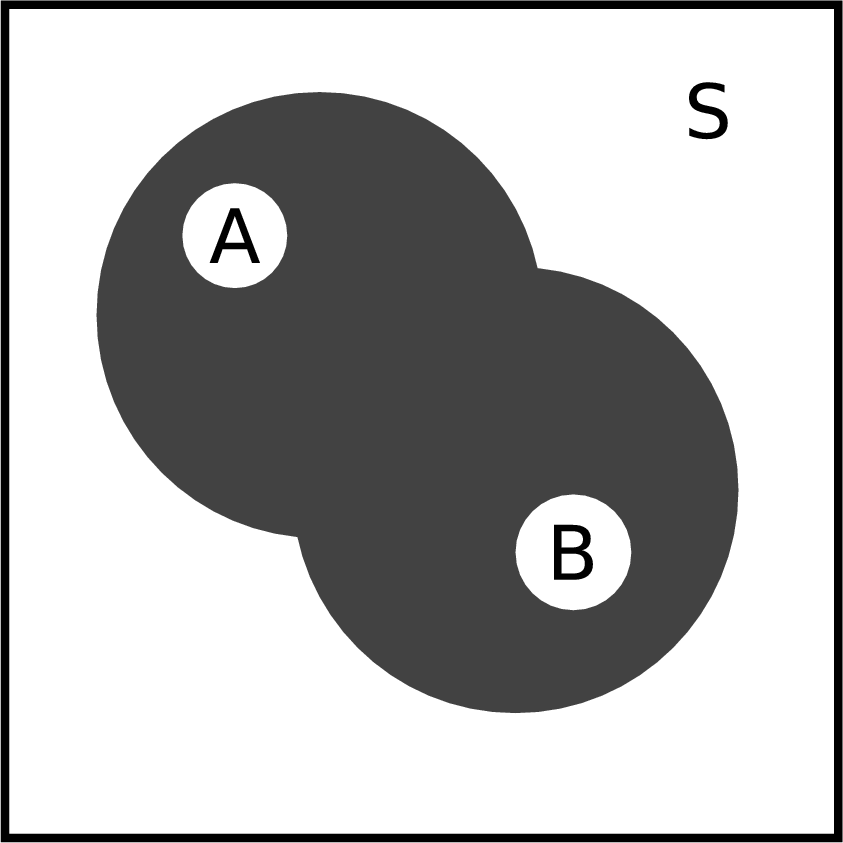
\includegraphics[width=80px]{col11306.imgs/m39373_union.png} % m39373;union.png;;;6.0;8.5;
        
      \vspace{2pt}
    \vspace{.1in}
    
    \end{center}



    \addtocounter{footnote}{-0}
    % make-rowspan-placeholders
    % rowspan info: col1 '0' | 'false' | '' || col2 '0' | 'false' | '' || col3 '0' | 'false' | '' || col4 '0' | 'false' | ''
     \tabularnewline\cline{1-1}\cline{2-2}\cline{3-3}\cline{4-4}
      %--------------------------------------------------------------------
    % align/colidx: left,1
    
    % rowcount: '0' | start: 'false' | colidx: '1'
    
        % Formatting a regular cell and recurring on the next sibling
        Intersection &
      % align/colidx: left,2
    
    % rowcount: '0' | start: 'false' | colidx: '2'
    
        % Formatting a regular cell and recurring on the next sibling
        Everything in A or B &
      % align/colidx: left,3
    
    % rowcount: '0' | start: 'false' | colidx: '3'
    
        % Formatting a regular cell and recurring on the next sibling
        \begin{math}A\cap B\end{math} &
      % align/colidx: left,4
    
    % rowcount: '0' | start: 'false' | colidx: '4'
    
        % Formatting a regular cell and recurring on the next sibling
        
    \setcounter{subfigure}{0}

\label{m39373*uid14587}
    \begin{center}
    \label{m39373*uid14587!!!underscore!!!media}\label{m39373*uid14587!!!underscore!!!printimage}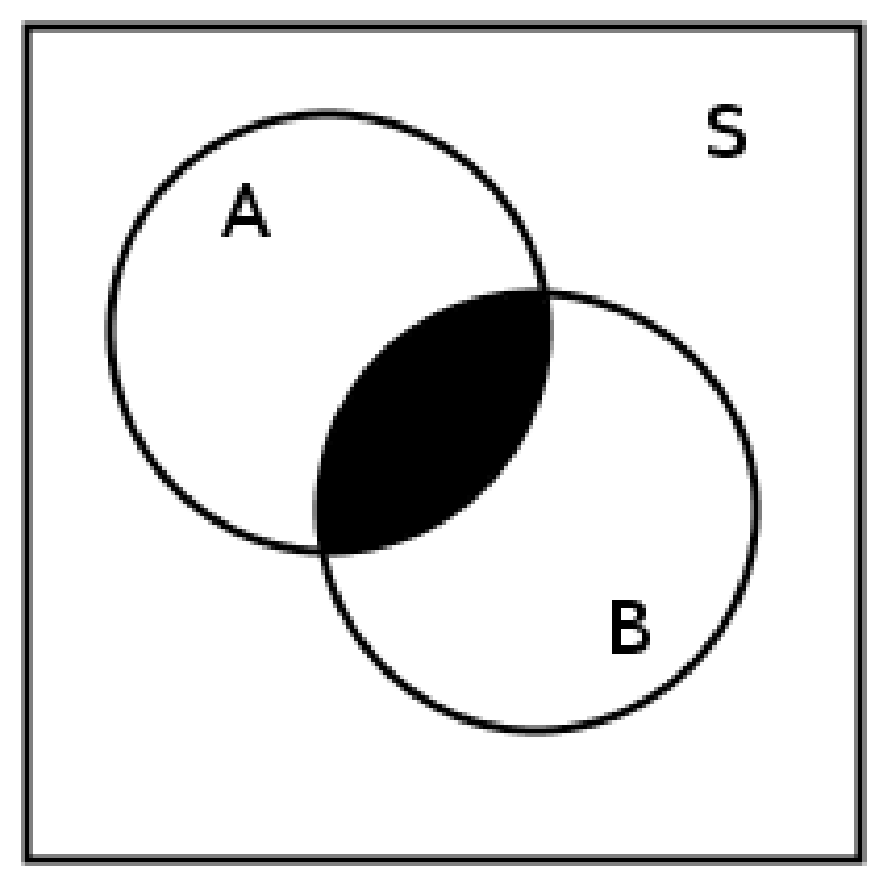
\includegraphics[width=80px]{col11306.imgs/m39373_intersect.png} % m39373;intersect.png;;;6.0;8.5;
        
      \vspace{2pt}
    \vspace{.1in}
    
    \end{center}



    \addtocounter{footnote}{-0}
    % make-rowspan-placeholders
    % rowspan info: col1 '0' | 'false' | '' || col2 '0' | 'false' | '' || col3 '0' | 'false' | '' || col4 '0' | 'false' | ''
     \tabularnewline\cline{1-1}\cline{2-2}\cline{3-3}\cline{4-4}
      %--------------------------------------------------------------------
    % align/colidx: left,1
    
    % rowcount: '0' | start: 'false' | colidx: '1'
    
        % Formatting a regular cell and recurring on the next sibling
        Complement &
      % align/colidx: left,2
    
    % rowcount: '0' | start: 'false' | colidx: '2'
    
        % Formatting a regular cell and recurring on the next sibling
        Everything that is not in A &
      % align/colidx: left,3
    
    % rowcount: '0' | start: 'false' | colidx: '3'
    
        % Formatting a regular cell and recurring on the next sibling
        \begin{math}{A}_{c}\end{math} &
      % align/colidx: left,4
    
    % rowcount: '0' | start: 'false' | colidx: '4'
    
        % Formatting a regular cell and recurring on the next sibling
         
    \setcounter{subfigure}{0}

\label{m39373*uid14567}
    \begin{center}
    \label{m39373*uid14567!!!underscore!!!media}\label{m39373*uid14567!!!underscore!!!printimage}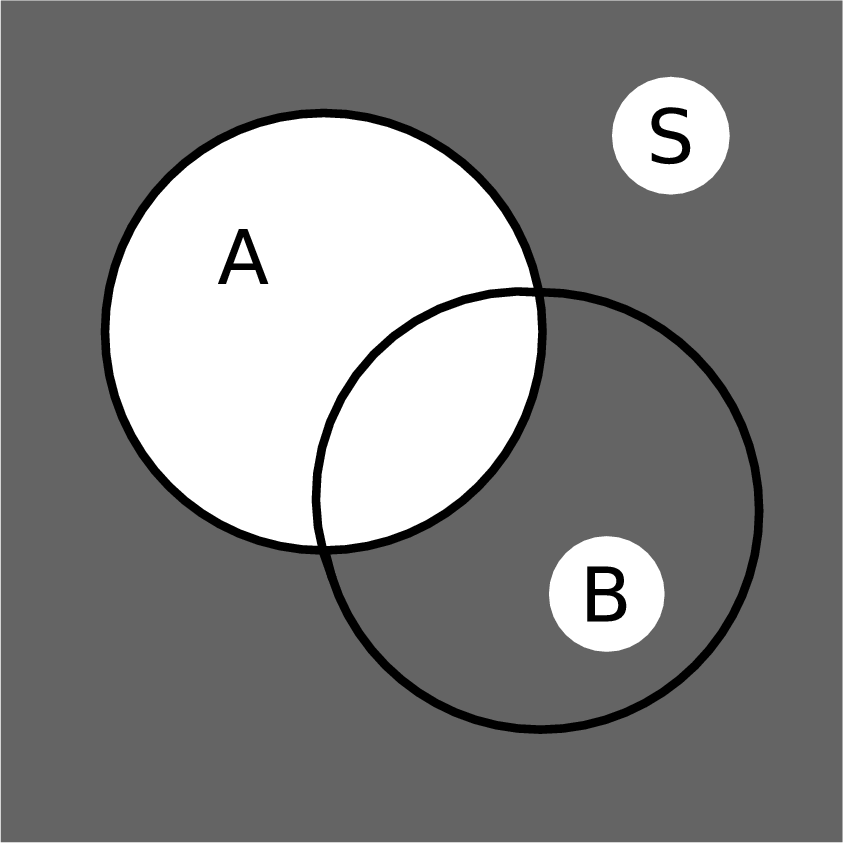
\includegraphics[width=80px]{col11306.imgs/m39373_complement.png} % m39373;complement.png;;;6.0;8.5;
        
      \vspace{2pt}
    \vspace{.1in}
    
    \end{center}



    \addtocounter{footnote}{-0}
    % make-rowspan-placeholders
    % rowspan info: col1 '0' | 'false' | '' || col2 '0' | 'false' | '' || col3 '0' | 'false' | '' || col4 '0' | 'false' | ''
     \tabularnewline\cline{1-1}\cline{2-2}\cline{3-3}\cline{4-4}
      %--------------------------------------------------------------------
    % align/colidx: left,1
    
    % rowcount: '0' | start: 'false' | colidx: '1'
    
        % Formatting a regular cell and recurring on the next sibling
        Only one &
      % align/colidx: left,2
    
    % rowcount: '0' | start: 'false' | colidx: '2'
    
        % Formatting a regular cell and recurring on the next sibling
        All that is only in A &
      % align/colidx: left,3
    
    % rowcount: '0' | start: 'false' | colidx: '3'
    
        % Formatting a regular cell and recurring on the next sibling
        \begin{math}A-B\end{math} &
      % align/colidx: left,4
    
    % rowcount: '0' | start: 'false' | colidx: '4'
    
        % Formatting a regular cell and recurring on the next sibling
        
    \setcounter{subfigure}{0}

\label{m39373*uid14767}
    \begin{center}
    \label{m39373*uid14767!!!underscore!!!media}\label{m39373*uid14767!!!underscore!!!printimage}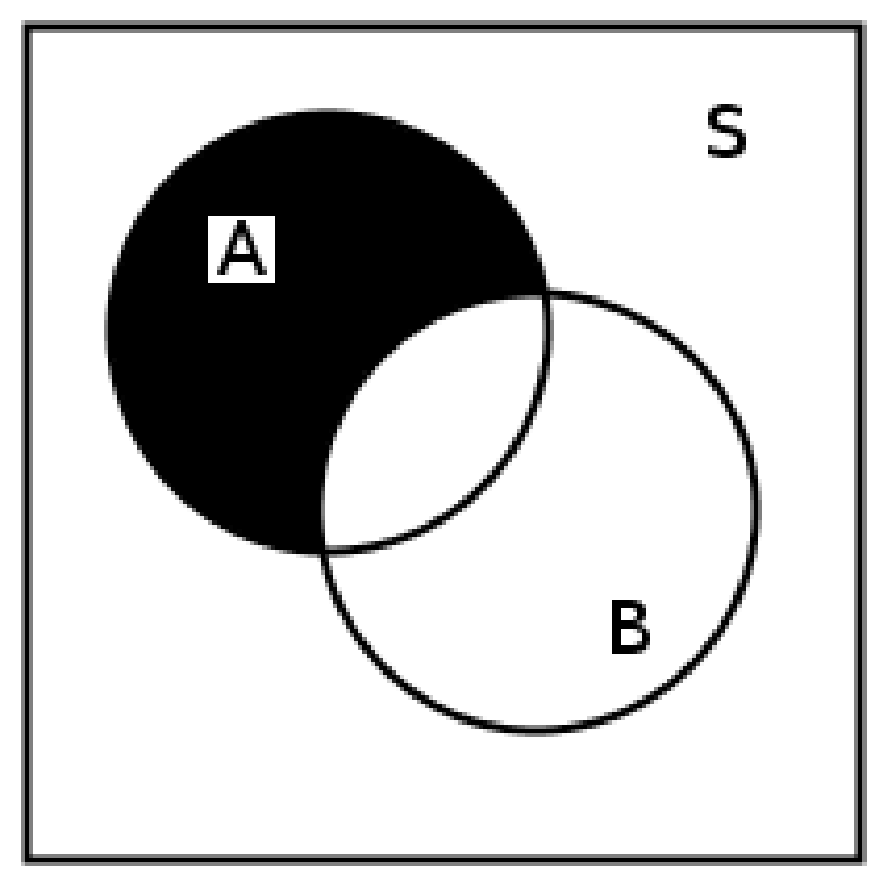
\includegraphics[width=80px]{col11306.imgs/m39373_a-b.png} % m39373;a-b.png;;;6.0;8.5;
        
      \vspace{2pt}
    \vspace{.1in}
    
    \end{center}



    \addtocounter{footnote}{-0}
    % make-rowspan-placeholders
    % rowspan info: col1 '0' | 'false' | '' || col2 '0' | 'false' | '' || col3 '0' | 'false' | '' || col4 '0' | 'false' | ''
     \tabularnewline\cline{1-1}\cline{2-2}\cline{3-3}\cline{4-4}
      %--------------------------------------------------------------------
    \end{xtabular*}
      \end{center}
    \begin{center}{\small\bfseries Table 11.5}\end{center}
    %\end{table}
    
    \addtocounter{footnote}{-0}
    
    \par
  \label{m39373*cid10}
            \section{ End of Chapter Exercises}
            \nopagebreak
            \label{m39373*id115876}\begin{enumerate}[noitemsep, label=\textbf{\arabic*}. ] 
            \label{m39373*uid104}\item A group of 45 children were asked if they eat Frosties and/or
Strawberry Pops. 31 eat both and 6 eat only Frosties. What is the probability
that a child chosen at random will eat only Strawberry Pops?\newline
            
\label{m39373*uid105}\item In a group of 42 pupils, all but 3 had a packet of
chips or a Fanta or both. If 23 had a packet of chips and 7 of these also had a
% Fanta, what is the probability that one pupil chosen at random has:     \section{ Probability: Part 2}
%     \nopagebreak
%             \label{m39373} $ \hspace{-5pt}\begin{array}{cccccccccccc}   
\includegraphics[width=0.75cm]{col11306.imgs/summary_fullmarks.png} &   \end{array} $ \hspace{2 pt}\raisebox{-5 pt}{} {(section shortcode: MG10086 )} \par 
%     
    
    
    
    
\label{m39373*id115906}\begin{enumerate}[noitemsep, label=\textbf{\alph*}. ] 
            \label{m39373*uid106}\item Both chips and Fanta
\label{m39373*uid107}\item has only Fanta?
\end{enumerate}
                \label{m39373*uid108}\item Use a Venn diagram to work out the following
probabilities from a die being rolled:
\label{m39373*id115948}\begin{enumerate}[noitemsep, label=\textbf{\alph*}. ] 
            \label{m39373*uid109}\item A multiple of 5 and an odd number
\label{m39373*uid110}\item a number that is neither a multiple of 5 nor an odd
number
\label{m39373*uid111}\item a number which is not a multiple of 5, but is odd.
\end{enumerate}
                \label{m39373*uid112}\item A packet has yellow and pink sweets. The probability
of taking out a pink sweet is 7/12.
\label{m39373*id116002}\begin{enumerate}[noitemsep, label=\textbf{\alph*}. ] 
            \label{m39373*uid113}\item What is the probability of taking
out a yellow sweet
\label{m39373*uid114}\item If 44 if the sweets are yellow, how many sweets are
pink?
\end{enumerate}
                \label{m39373*uid115}\item In a car park with 300 cars, there are 190 Opels. What
is the probability that the first car to leave the car park is:
\label{m39373*id116044}\begin{enumerate}[noitemsep, label=\textbf{\alph*}. ] 
            \label{m39373*uid116}\item an Opel
\label{m39373*uid117}\item not an Opel
\end{enumerate}
                \label{m39373*uid118}\item Tamara has 18 loose socks in a drawer. Eight of these
are orange and two are pink. Calculate the probability that the first sock taken
out at random is:
\label{m39373*id116086}\begin{enumerate}[noitemsep, label=\textbf{\alph*}. ] 
            \label{m39373*uid119}\item Orange
\label{m39373*uid120}\item not orange
% \label{m39373*uid121}\item pink     \section{ Probability: Part 2}
%     \nopagebreak
%             \label{m39373} $ \hspace{-5pt}\begin{array}{cccccccccccc}   
\includegraphics[width=0.75cm]{col11306.imgs/summary_fullmarks.png} &   \end{array} $ \hspace{2 pt}\raisebox{-5 pt}{} {(section shortcode: MG10086 )} \par 
%     
    
    
    
    
\label{m39373*uid122}\item not pink
\label{m39373*uid123}\item orange or pink
\label{m39373*uid124}\item not orange or pink
\end{enumerate}
                \label{m39373*uid125}\item A plate contains 9 shortbread cookies, 4 ginger
biscuits, 11 chocolate chip cookies and 18 Jambos. If a biscuit is selected at
random, what is the probability that:
\label{m39373*id116177}\begin{enumerate}[noitemsep, label=\textbf{\alph*}. ] 
            \label{m39373*uid126}\item it is either a ginger biscuit of a
Jambo?
\label{m39373*uid127}\item it is NOT a shortbread cookie.
\end{enumerate}
                \label{m39373*uid128}\item 280 tickets were sold at a raffle. Ingrid bought 15
tickets. What is the probability that Ingrid:
\label{m39373*id116219}\begin{enumerate}[noitemsep, label=\textbf{\alph*}. ] 
            \label{m39373*uid129}\item Wins the prize
\label{m39373*uid130}\item Does not win the prize?
\end{enumerate}
                \label{m39373*uid131}\item The children in a nursery school were classified by
hair and eye colour. 44 had red hair and not brown eyes, 14 had brown eyes and
red hair, 5 had brown eyes but not red hair and 40 did not have brown eyes or
red hair.
\label{m39373*id116261}\begin{enumerate}[noitemsep, label=\textbf{\alph*}. ] 
            \label{m39373*uid132}\item How many children were in the
school
\label{m39373*uid133}\item What is the probility that a child chosen at random
has:
\label{m39373*id116289}\begin{enumerate}[noitemsep, label=\textbf{\arabic*}. ] 
            \label{m39373*uid134}\item Brown eyes
\label{m39373*uid135}\item Red hair
% \end{enumerate}     \section{ Probability: Part 2}
%     \nopagebreak
%             \label{m39373} $ \hspace{-5pt}\begin{array}{cccccccccccc}   
\includegraphics[width=0.75cm]{col11306.imgs/summary_fullmarks.png} &   \end{array} $ \hspace{2 pt}\raisebox{-5 pt}{} {(section shortcode: MG10086 )} \par 
%     
    
    
    
    
        \label{m39373*uid136}\item A child with brown eyes is chosen
randomly. What is the probability that this child will have red hair
\end{enumerate}
                \label{m39373*uid137}\item A jar has purple, blue and black sweets in it. The
probability that a sweet, chosen at random, will be purple is 1/7 and the
probability that it will be black is 3/5.
\label{m39373*id116346}\begin{enumerate}[noitemsep, label=\textbf{\alph*}. ] 
            \label{m39373*uid138}\item If I choose a sweet at random what
is the probability that it will be:
\label{m39373*id116362}\begin{enumerate}[noitemsep, label=\textbf{\roman*}. ] 
            \label{m39373*uid139}\item purple or blue
\label{m39373*uid140}\item Black
\label{m39373*uid141}\item purple
\end{enumerate}
        \label{m39373*uid142}\item If there are 70 sweets in the jar how
many purple ones are there?
\label{m39373*uid143}\item 1/4 if the purple sweets in b) have streaks on them and
rest do not. How many purple sweets have streaks?
\end{enumerate}
                \label{m39373*uid144}\item For each of the following, draw a Venn diagram to
represent the situation and find an example to illustrate the situation.
\label{m39373*id116443}\begin{enumerate}[noitemsep, label=\textbf{\alph*}. ] 
            \label{m39373*uid145}\item A sample space in which there are
two events that are not mutually exclusive
\label{m39373*uid146}\item A sample space in which there are two events that are
complementary.
\end{enumerate}
                \label{m39373*uid147}\item Use a Venn diagram to prove that the probability of
either event A or B occuring is given by: (A and B are not exclusive)
P(A or B) = P(A) + P(B) - P(A and B)\newline
            
\label{m39373*uid148}\item All the clubs are taken out of a pack of cards. The
remaining cards are then shuffled and one card chosen. After being chosen, the
card is replaced before the next card is chosen.
\label{m39373*id116505}\begin{enumerate}[noitemsep, label=\textbf{\alph*}. ] 
            \label{m39373*uid149}\item What is the sample space?
\label{m39373*uid150}\item Find a set to represent the event, P, of drawing a
picture card.
\label{m39373*uid151}\item Find a set for the event, N, of drawing a numbered
card.
\label{m39373*uid152}\item Represent the above events in a Venn diagram
\label{m39373*uid153}\item What description of the sets P and N is suitable?
(Hint: Find any elements of P in N and N in P.)
\end{enumerate}
                \label{m39373*uid154}\item Thuli has a bag containing five orange, three purple
and seven pink blocks. The bag is shaken and a block is withdrawn. The colour of
the block is noted and the block is replaced.
\label{m39373*id116586}\begin{enumerate}[noitemsep, label=\textbf{\alph*}. ] 
            \label{m39373*uid155}\item What is the sample space for this
experiment?
\label{m39373*uid156}\item What is the set describing the event of drawing a pink
block, P?
\label{m39373*uid157}\item Write down a set, O or B, to represent the event of
drawing either a orange or a purple block.
\label{m39373*uid158}\item Draw a Venn diagram to show the above information.
\end{enumerate}
                \end{enumerate}
        
    
  \label{m39373**end}
          
       
    
  \label{0bb9905f9f275884255abbf74a951a4a**end}
    
\par \raisebox{-5 pt}{
\includegraphics[width=0.5cm]{col11306.imgs/summary_www.png}} Find the answers with the shortcodes:
 \par \begin{tabular}[h]{cccccc}
 (1.) lqh  &  (2.) llq  &  (3.) lll  &  (4.) lli  &  (5.) ll3  &  (6.) llO  &  (7.) llc  &  (8.) llx  &  (9.) lla  &  (10.) llC  &  (11.) ll1  &  (12.) llr  &  (13.) llY  &  (14.) llg  & \end{tabular}



